\documentclass[twoside]{book}

% Packages required by doxygen
\usepackage{fixltx2e}
\usepackage{calc}
\usepackage{doxygen}
\usepackage[export]{adjustbox} % also loads graphicx
\usepackage{graphicx}
\usepackage[utf8]{inputenc}
\usepackage{makeidx}
\usepackage{multicol}
\usepackage{multirow}
\PassOptionsToPackage{warn}{textcomp}
\usepackage{textcomp}
\usepackage[nointegrals]{wasysym}
\usepackage[table]{xcolor}

% Font selection
\usepackage[T1]{fontenc}
\usepackage[scaled=.90]{helvet}
\usepackage{courier}
\usepackage{amssymb}
\usepackage{sectsty}
\renewcommand{\familydefault}{\sfdefault}
\allsectionsfont{%
  \fontseries{bc}\selectfont%
  \color{darkgray}%
}
\renewcommand{\DoxyLabelFont}{%
  \fontseries{bc}\selectfont%
  \color{darkgray}%
}
\newcommand{\+}{\discretionary{\mbox{\scriptsize$\hookleftarrow$}}{}{}}

% Page & text layout
\usepackage{geometry}
\geometry{%
  a4paper,%
  top=2.5cm,%
  bottom=2.5cm,%
  left=2.5cm,%
  right=2.5cm%
}
\tolerance=750
\hfuzz=15pt
\hbadness=750
\setlength{\emergencystretch}{15pt}
\setlength{\parindent}{0cm}
\setlength{\parskip}{3ex plus 2ex minus 2ex}
\makeatletter
\renewcommand{\paragraph}{%
  \@startsection{paragraph}{4}{0ex}{-1.0ex}{1.0ex}{%
    \normalfont\normalsize\bfseries\SS@parafont%
  }%
}
\renewcommand{\subparagraph}{%
  \@startsection{subparagraph}{5}{0ex}{-1.0ex}{1.0ex}{%
    \normalfont\normalsize\bfseries\SS@subparafont%
  }%
}
\makeatother

% Headers & footers
\usepackage{fancyhdr}
\pagestyle{fancyplain}
\fancyhead[LE]{\fancyplain{}{\bfseries\thepage}}
\fancyhead[CE]{\fancyplain{}{}}
\fancyhead[RE]{\fancyplain{}{\bfseries\leftmark}}
\fancyhead[LO]{\fancyplain{}{\bfseries\rightmark}}
\fancyhead[CO]{\fancyplain{}{}}
\fancyhead[RO]{\fancyplain{}{\bfseries\thepage}}
\fancyfoot[LE]{\fancyplain{}{}}
\fancyfoot[CE]{\fancyplain{}{}}
\fancyfoot[RE]{\fancyplain{}{\bfseries\scriptsize 制作者 Doxygen }}
\fancyfoot[LO]{\fancyplain{}{\bfseries\scriptsize 制作者 Doxygen }}
\fancyfoot[CO]{\fancyplain{}{}}
\fancyfoot[RO]{\fancyplain{}{}}
\renewcommand{\footrulewidth}{0.4pt}
\renewcommand{\chaptermark}[1]{%
  \markboth{#1}{}%
}
\renewcommand{\sectionmark}[1]{%
  \markright{\thesection\ #1}%
}

% Indices & bibliography
\usepackage{natbib}
\usepackage[titles]{tocloft}
\setcounter{tocdepth}{3}
\setcounter{secnumdepth}{5}
\makeindex

% Hyperlinks (required, but should be loaded last)
\usepackage{ifpdf}
\ifpdf
  \usepackage[pdftex,pagebackref=true]{hyperref}
\else
  \usepackage[ps2pdf,pagebackref=true]{hyperref}
\fi
\hypersetup{%
  colorlinks=true,%
  linkcolor=blue,%
  citecolor=blue,%
  unicode%
}

% Custom commands
\newcommand{\clearemptydoublepage}{%
  \newpage{\pagestyle{empty}\cleardoublepage}%
}

\usepackage{caption}
\captionsetup{labelsep=space,justification=centering,font={bf},singlelinecheck=off,skip=4pt,position=top}

%===== C O N T E N T S =====

\begin{document}

% Titlepage & ToC
\hypersetup{pageanchor=false,
             bookmarksnumbered=true,
             pdfencoding=unicode
            }
\pagenumbering{alph}
\begin{titlepage}
\vspace*{7cm}
\begin{center}%
{\Large Kylin S\+A\+NE A\+PI }\\
\vspace*{1cm}
{\large 制作者 Doxygen 1.8.13}\\
\end{center}
\end{titlepage}
\clearemptydoublepage
\pagenumbering{roman}
\tableofcontents
\clearemptydoublepage
\pagenumbering{arabic}
\hypersetup{pageanchor=true}

%--- Begin generated contents ---
\chapter{Simple Linux S\+A\+NE Scanning Application in C}
\label{md_README}
\Hypertarget{md_README}
\+:earth\+\_\+asia\+: \+:cn\+:

The sample demonstrates how to implement a simple document scanning application on Linux in C. Switch to chinese \+:arrow\+\_\+right\+: \hyperlink{md_README_CN}{chinese}

\subsection*{Getting Started}


\begin{DoxyEnumerate}
\item Install S\+A\+NE\+:

``` sudo apt-\/get update sudo apt-\/get install sane sudo apt-\/get install sane-\/utils sudo apt-\/get install libsane-\/dev ```
\item Download \href{https://alioth.debian.org/frs/?group_id=30186}{\tt sane-\/backends-\/1.\+0.\+25}. This is not necessary.
\item Extract the package and generate a symlink\+:

Ubuntu

```bash sudo ln –s /usr/lib/x86\+\_\+64-\/linux-\/gnu/libsane.so.\+1 /usr/lib/libsane.so ```
\item Get the source code and change the include path\+:

``` S\+A\+N\+E\+\_\+\+I\+N\+C\+L\+U\+DE=$<$\+Your sane=\char`\"{}\char`\"{} package=\char`\"{}\char`\"{} path$>$=\char`\"{}\char`\"{}$>$/include ```

default\+: S\+A\+N\+E\+\_\+\+I\+N\+C\+L\+U\+DE=/usr/include
\item Build the project\+: ``` make ```
\item Run the application\+:

``` sudo ./kylin\+Sane ```
\item Preview docs on web

``` firefox docs/html/index.\+html or \href{file:///home/yusq/sane-test/docs/html/index.html}{\tt file\+:///home/yusq/sane-\/test/docs/html/index.\+html} ``` call main graph\+: 
\end{DoxyEnumerate}

\subsection*{Reference}


\begin{DoxyItemize}
\item \href{http://www.sane-project.org/docs.html}{\tt S\+A\+NE -\/ Documentation}
\item \href{https://github.com/yushulx/linux-document-scanning}{\tt S\+A\+NE -\/ Other github}
\item \href{https://blog.csdn.net/weixin_39743893/article/details/83350568}{\tt S\+A\+NE -\/ Documentation CN} 
\end{DoxyItemize}
\chapter{简单扫描\+S\+A\+NE A\+PI 使用}
\label{md_README_CN}
\Hypertarget{md_README_CN}
\#\# 开始安装\+S\+A\+N\+E及对应的开发库 
\begin{DoxyCode}
sudo apt-get update
sudo apt-get sane sane-utils libsane-dev

sudo ln -s /usr/lib/x86\_64-linux-gnu/libsane.so.1 /usr/lib/libsane.so
\end{DoxyCode}


\subsection*{源码演示}


\begin{DoxyEnumerate}
\item 更改\+Makefile的头文件路径 
\begin{DoxyCode}
SANE\_INCLUDE=/home/yusq/kylin-sane-test/include/
\end{DoxyCode}

\item 编译并执行 
\begin{DoxyCode}
make
./kylinSane
\end{DoxyCode}

\item 在线文档查看 
\begin{DoxyCode}
firefox docs/html/index.html
or
file:///home/yusq/sane-test/docs/html/index.html
\end{DoxyCode}

\end{DoxyEnumerate}

\subsection*{参考文档}


\begin{DoxyItemize}
\item \href{http://www.sane-project.org/docs.html}{\tt S\+A\+NE -\/ Documentation}
\item \href{https://github.com/yushulx/linux-document-scanning}{\tt S\+A\+NE -\/ Other github}
\item \href{https://blog.csdn.net/weixin_39743893/article/details/83350568}{\tt S\+A\+NE -\/ Documentation CN} 
\end{DoxyItemize}
\chapter{结构体索引}
\doxysection{结构体}
这里列出了所有结构体,并附带简要说明\+:\begin{DoxyCompactList}
\item\contentsline{section}{\mbox{\hyperlink{structImage}{Image}} }{\pageref{structImage}}{}
\item\contentsline{section}{\mbox{\hyperlink{structSANE__Device}{S\+A\+N\+E\+\_\+\+Device}} }{\pageref{structSANE__Device}}{}
\item\contentsline{section}{\mbox{\hyperlink{structSANE__Option__Descriptor}{S\+A\+N\+E\+\_\+\+Option\+\_\+\+Descriptor}} }{\pageref{structSANE__Option__Descriptor}}{}
\item\contentsline{section}{\mbox{\hyperlink{structSANE__Parameters}{S\+A\+N\+E\+\_\+\+Parameters}} }{\pageref{structSANE__Parameters}}{}
\item\contentsline{section}{\mbox{\hyperlink{structSANE__Range}{S\+A\+N\+E\+\_\+\+Range}} }{\pageref{structSANE__Range}}{}
\end{DoxyCompactList}

\chapter{文件索引}
\doxysection{文件列表}
这里列出了所有文件,并附带简要说明\+:\begin{DoxyCompactList}
\item\contentsline{section}{\mbox{\hyperlink{kylin__sane_8cpp}{kylin\+\_\+sane.\+cpp}} }{\pageref{kylin__sane_8cpp}}{}
\item\contentsline{section}{\mbox{\hyperlink{kylin__sane_8h}{kylin\+\_\+sane.\+h}} }{\pageref{kylin__sane_8h}}{}
\item\contentsline{section}{\mbox{\hyperlink{main_8cpp}{main.\+cpp}} }{\pageref{main_8cpp}}{}
\item\contentsline{section}{include/sane/\mbox{\hyperlink{sane_8h}{sane.\+h}} \\*Sane.\+h A\+P\+I规范文档 }{\pageref{sane_8h}}{}
\item\contentsline{section}{include/sane/\mbox{\hyperlink{saneopts_8h}{saneopts.\+h}} }{\pageref{saneopts_8h}}{}
\end{DoxyCompactList}

\chapter{结构体说明}
\hypertarget{structImage}{}\section{Image结构体 参考}
\label{structImage}\index{Image@{Image}}
\subsection*{成员变量}
\begin{DoxyCompactItemize}
\item 
uint8\+\_\+t $\ast$ \hyperlink{structImage_ac149fdf39be15025af7c3d8659f80999}{data}
\item 
int \hyperlink{structImage_ab8d12f635013c04159cd4d3d972bac88}{width}
\item 
int \hyperlink{structImage_a51df43db420c9c0b57536cb2dd36de5c}{height}
\item 
int \hyperlink{structImage_a7f8f4530212c93856e611030e46c82af}{x}
\item 
int \hyperlink{structImage_a9b03b7d8dd6f69cb5a444bdd0edd786e}{y}
\end{DoxyCompactItemize}


\subsection{结构体成员变量说明}
\mbox{\Hypertarget{structImage_ac149fdf39be15025af7c3d8659f80999}\label{structImage_ac149fdf39be15025af7c3d8659f80999}} 
\index{Image@{Image}!data@{data}}
\index{data@{data}!Image@{Image}}
\subsubsection{\texorpdfstring{data}{data}}
{\footnotesize\ttfamily uint8\+\_\+t$\ast$ Image\+::data}

\mbox{\Hypertarget{structImage_a51df43db420c9c0b57536cb2dd36de5c}\label{structImage_a51df43db420c9c0b57536cb2dd36de5c}} 
\index{Image@{Image}!height@{height}}
\index{height@{height}!Image@{Image}}
\subsubsection{\texorpdfstring{height}{height}}
{\footnotesize\ttfamily int Image\+::height}

\mbox{\Hypertarget{structImage_ab8d12f635013c04159cd4d3d972bac88}\label{structImage_ab8d12f635013c04159cd4d3d972bac88}} 
\index{Image@{Image}!width@{width}}
\index{width@{width}!Image@{Image}}
\subsubsection{\texorpdfstring{width}{width}}
{\footnotesize\ttfamily int Image\+::width}

\mbox{\Hypertarget{structImage_a7f8f4530212c93856e611030e46c82af}\label{structImage_a7f8f4530212c93856e611030e46c82af}} 
\index{Image@{Image}!x@{x}}
\index{x@{x}!Image@{Image}}
\subsubsection{\texorpdfstring{x}{x}}
{\footnotesize\ttfamily int Image\+::x}

\mbox{\Hypertarget{structImage_a9b03b7d8dd6f69cb5a444bdd0edd786e}\label{structImage_a9b03b7d8dd6f69cb5a444bdd0edd786e}} 
\index{Image@{Image}!y@{y}}
\index{y@{y}!Image@{Image}}
\subsubsection{\texorpdfstring{y}{y}}
{\footnotesize\ttfamily int Image\+::y}



该结构体的文档由以下文件生成\+:\begin{DoxyCompactItemize}
\item 
\hyperlink{kylin__sane_8c}{kylin\+\_\+sane.\+c}\end{DoxyCompactItemize}

\hypertarget{structoption}{}\doxysection{option结构体 参考}
\label{structoption}\index{option@{option}}
\doxysubsection*{成员变量}
\begin{DoxyCompactItemize}
\item 
char $\ast$ \mbox{\hyperlink{structoption_a92c850a23c7828c1dba453bf8d15e1f0}{name}}
\item 
int \mbox{\hyperlink{structoption_a90d7ee9a51eea5c002682dbd0af149e4}{has\+\_\+arg}}
\item 
int $\ast$ \mbox{\hyperlink{structoption_ab366eea5fe7be25c1928328ba715e353}{flag}}
\item 
int \mbox{\hyperlink{structoption_a13bd155ec3b405d29c41ab8d0793be11}{val}}
\end{DoxyCompactItemize}


\doxysubsection{结构体成员变量说明}
\mbox{\Hypertarget{structoption_ab366eea5fe7be25c1928328ba715e353}\label{structoption_ab366eea5fe7be25c1928328ba715e353}} 
\index{option@{option}!flag@{flag}}
\index{flag@{flag}!option@{option}}
\doxysubsubsection{\texorpdfstring{flag}{flag}}
{\footnotesize\ttfamily int$\ast$ option\+::flag}

\mbox{\Hypertarget{structoption_a90d7ee9a51eea5c002682dbd0af149e4}\label{structoption_a90d7ee9a51eea5c002682dbd0af149e4}} 
\index{option@{option}!has\_arg@{has\_arg}}
\index{has\_arg@{has\_arg}!option@{option}}
\doxysubsubsection{\texorpdfstring{has\_arg}{has\_arg}}
{\footnotesize\ttfamily int option\+::has\+\_\+arg}

\mbox{\Hypertarget{structoption_a92c850a23c7828c1dba453bf8d15e1f0}\label{structoption_a92c850a23c7828c1dba453bf8d15e1f0}} 
\index{option@{option}!name@{name}}
\index{name@{name}!option@{option}}
\doxysubsubsection{\texorpdfstring{name}{name}}
{\footnotesize\ttfamily char$\ast$ option\+::name}

\mbox{\Hypertarget{structoption_a13bd155ec3b405d29c41ab8d0793be11}\label{structoption_a13bd155ec3b405d29c41ab8d0793be11}} 
\index{option@{option}!val@{val}}
\index{val@{val}!option@{option}}
\doxysubsubsection{\texorpdfstring{val}{val}}
{\footnotesize\ttfamily int option\+::val}



该结构体的文档由以下文件生成\+:\begin{DoxyCompactItemize}
\item 
\mbox{\hyperlink{main_8cpp}{main.\+cpp}}\end{DoxyCompactItemize}

\hypertarget{structSANE__Device}{}\section{S\+A\+N\+E\+\_\+\+Device结构体 参考}
\label{structSANE__Device}\index{S\+A\+N\+E\+\_\+\+Device@{S\+A\+N\+E\+\_\+\+Device}}


{\ttfamily \#include $<$sane.\+h$>$}

\subsection*{成员变量}
\begin{DoxyCompactItemize}
\item 
\hyperlink{sane_8h_a9a47323dab2a36db080f1bcc11585af4}{S\+A\+N\+E\+\_\+\+String\+\_\+\+Const} \hyperlink{structSANE__Device_a6ade6e5e2cf659520c0ceae0c50adc55}{name}
\item 
\hyperlink{sane_8h_a9a47323dab2a36db080f1bcc11585af4}{S\+A\+N\+E\+\_\+\+String\+\_\+\+Const} \hyperlink{structSANE__Device_a30329d1b829b0d7308c31e18f8a81ccf}{vendor}
\item 
\hyperlink{sane_8h_a9a47323dab2a36db080f1bcc11585af4}{S\+A\+N\+E\+\_\+\+String\+\_\+\+Const} \hyperlink{structSANE__Device_a053a3964744fbd7a304c00332678e200}{model}
\item 
\hyperlink{sane_8h_a9a47323dab2a36db080f1bcc11585af4}{S\+A\+N\+E\+\_\+\+String\+\_\+\+Const} \hyperlink{structSANE__Device_ac66eea9d60c35fea4af804e6fecbe473}{type}
\end{DoxyCompactItemize}


\subsection{详细描述}
设备描述符类型 每个\+S\+A\+N\+E设备都由\+S\+A\+N\+E\+\_\+\+Device类型的结构表示 该结构在成员名称中提供了扫描仪的唯一 名称。设备结构中的其余成员在设备上提供了与唯一名称相对应的其他信息。 在调用sane\+\_\+open()时应传递此唯一名称。此名称的格式完全取决于后端。 唯一的限制是该名称在后端支持的所有设备中都是唯一的,并且该名称是合法的\+S\+A\+N\+E文本字符串。 为了简化唯一名称的表示,其长度不应过多。这是建议的是后端保持低于长度为32个字符的唯一名称。 但是,应用程序 必须能够处理任意长度的唯一名称。 供应商字符串\+Noname可以用于没有物理供应商关联的虚拟设备。 而且,由于这些字符串是特定于供应商的,因此没有预定义的型号名称字符串,因此完全在各个后端的控制之下。 

\subsection{结构体成员变量说明}
\mbox{\Hypertarget{structSANE__Device_a053a3964744fbd7a304c00332678e200}\label{structSANE__Device_a053a3964744fbd7a304c00332678e200}} 
\index{S\+A\+N\+E\+\_\+\+Device@{S\+A\+N\+E\+\_\+\+Device}!model@{model}}
\index{model@{model}!S\+A\+N\+E\+\_\+\+Device@{S\+A\+N\+E\+\_\+\+Device}}
\subsubsection{\texorpdfstring{model}{model}}
{\footnotesize\ttfamily \hyperlink{sane_8h_a9a47323dab2a36db080f1bcc11585af4}{S\+A\+N\+E\+\_\+\+String\+\_\+\+Const} S\+A\+N\+E\+\_\+\+Device\+::model}

device model name, 型号 \mbox{\Hypertarget{structSANE__Device_a6ade6e5e2cf659520c0ceae0c50adc55}\label{structSANE__Device_a6ade6e5e2cf659520c0ceae0c50adc55}} 
\index{S\+A\+N\+E\+\_\+\+Device@{S\+A\+N\+E\+\_\+\+Device}!name@{name}}
\index{name@{name}!S\+A\+N\+E\+\_\+\+Device@{S\+A\+N\+E\+\_\+\+Device}}
\subsubsection{\texorpdfstring{name}{name}}
{\footnotesize\ttfamily \hyperlink{sane_8h_a9a47323dab2a36db080f1bcc11585af4}{S\+A\+N\+E\+\_\+\+String\+\_\+\+Const} S\+A\+N\+E\+\_\+\+Device\+::name}

unique device name, 有关卖方(制造商名字) \mbox{\Hypertarget{structSANE__Device_ac66eea9d60c35fea4af804e6fecbe473}\label{structSANE__Device_ac66eea9d60c35fea4af804e6fecbe473}} 
\index{S\+A\+N\+E\+\_\+\+Device@{S\+A\+N\+E\+\_\+\+Device}!type@{type}}
\index{type@{type}!S\+A\+N\+E\+\_\+\+Device@{S\+A\+N\+E\+\_\+\+Device}}
\subsubsection{\texorpdfstring{type}{type}}
{\footnotesize\ttfamily \hyperlink{sane_8h_a9a47323dab2a36db080f1bcc11585af4}{S\+A\+N\+E\+\_\+\+String\+\_\+\+Const} S\+A\+N\+E\+\_\+\+Device\+::type}

device type (e.\+g., \char`\"{}flatbed scanner\char`\"{}), 设备类型 \mbox{\Hypertarget{structSANE__Device_a30329d1b829b0d7308c31e18f8a81ccf}\label{structSANE__Device_a30329d1b829b0d7308c31e18f8a81ccf}} 
\index{S\+A\+N\+E\+\_\+\+Device@{S\+A\+N\+E\+\_\+\+Device}!vendor@{vendor}}
\index{vendor@{vendor}!S\+A\+N\+E\+\_\+\+Device@{S\+A\+N\+E\+\_\+\+Device}}
\subsubsection{\texorpdfstring{vendor}{vendor}}
{\footnotesize\ttfamily \hyperlink{sane_8h_a9a47323dab2a36db080f1bcc11585af4}{S\+A\+N\+E\+\_\+\+String\+\_\+\+Const} S\+A\+N\+E\+\_\+\+Device\+::vendor}

device vendor string, 制造商 

该结构体的文档由以下文件生成\+:\begin{DoxyCompactItemize}
\item 
include/sane/\hyperlink{sane_8h}{sane.\+h}\end{DoxyCompactItemize}

\hypertarget{structSANE__Option__Descriptor}{}\doxysection{S\+A\+N\+E\+\_\+\+Option\+\_\+\+Descriptor结构体 参考}
\label{structSANE__Option__Descriptor}\index{SANE\_Option\_Descriptor@{SANE\_Option\_Descriptor}}


{\ttfamily \#include $<$sane.\+h$>$}



S\+A\+N\+E\+\_\+\+Option\+\_\+\+Descriptor 的协作图\+:\nopagebreak
\begin{figure}[H]
\begin{center}
\leavevmode
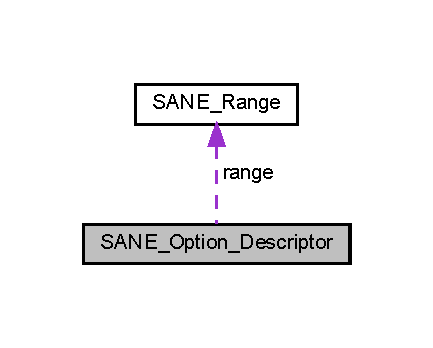
\includegraphics[width=208pt]{structSANE__Option__Descriptor__coll__graph}
\end{center}
\end{figure}
\doxysubsection*{成员变量}
\begin{DoxyCompactItemize}
\item 
\mbox{\hyperlink{sane_8h_a9a47323dab2a36db080f1bcc11585af4}{S\+A\+N\+E\+\_\+\+String\+\_\+\+Const}} \mbox{\hyperlink{structSANE__Option__Descriptor_ac4155621a2154ad3160c415fef6ca643}{name}}
\item 
\mbox{\hyperlink{sane_8h_a9a47323dab2a36db080f1bcc11585af4}{S\+A\+N\+E\+\_\+\+String\+\_\+\+Const}} \mbox{\hyperlink{structSANE__Option__Descriptor_a069392f9b5739153679dcccfd2bb50fe}{title}}
\item 
\mbox{\hyperlink{sane_8h_a9a47323dab2a36db080f1bcc11585af4}{S\+A\+N\+E\+\_\+\+String\+\_\+\+Const}} \mbox{\hyperlink{structSANE__Option__Descriptor_a668582efe29f5a4c9aab395afcd6ea18}{desc}}
\item 
\mbox{\hyperlink{sane_8h_aed3324dea8f24f5381e12e5562aaf72b}{S\+A\+N\+E\+\_\+\+Value\+\_\+\+Type}} \mbox{\hyperlink{structSANE__Option__Descriptor_a0f7c7e0902094d466389a82671b5b150}{type}}
\item 
\mbox{\hyperlink{sane_8h_a15e903425f365e0fe30fed1e37446990}{S\+A\+N\+E\+\_\+\+Unit}} \mbox{\hyperlink{structSANE__Option__Descriptor_a25b4534fcc925c6f316a3f180ec34435}{unit}}
\item 
\mbox{\hyperlink{sane_8h_a18b0de32eae6997909ae9ab0117af3d5}{S\+A\+N\+E\+\_\+\+Int}} \mbox{\hyperlink{structSANE__Option__Descriptor_a9b1f811d7c85d008d8a60e0b8d3e4a25}{size}}
\item 
\mbox{\hyperlink{sane_8h_a18b0de32eae6997909ae9ab0117af3d5}{S\+A\+N\+E\+\_\+\+Int}} \mbox{\hyperlink{structSANE__Option__Descriptor_a884b023bc72593766267a98ee0333607}{cap}}
\item 
\mbox{\hyperlink{sane_8h_a6422f68f593477ab1fd81078e9afc8e9}{S\+A\+N\+E\+\_\+\+Constraint\+\_\+\+Type}} \mbox{\hyperlink{structSANE__Option__Descriptor_a10767a0944d00b3dad2de45086512e76}{constraint\+\_\+type}}
\item 
\begin{tabbing}
xx\=xx\=xx\=xx\=xx\=xx\=xx\=xx\=xx\=\kill
union \{\\
\>const \mbox{\hyperlink{sane_8h_a9a47323dab2a36db080f1bcc11585af4}{SANE\_String\_Const}} $\ast$ \mbox{\hyperlink{structSANE__Option__Descriptor_a9526628ce75d40ebb74cc917dc919fde}{string\_list}}\\
\>const \mbox{\hyperlink{sane_8h_aa65d63e57d37984b9d873811a7544b4a}{SANE\_Word}} $\ast$ \mbox{\hyperlink{structSANE__Option__Descriptor_af23d6a521f5ae9e57bdbda3e3bfb7526}{word\_list}}\\
\>const \mbox{\hyperlink{structSANE__Range}{SANE\_Range}} $\ast$ \mbox{\hyperlink{structSANE__Option__Descriptor_a0f1bd3fe216630e36c84896ac384a233}{range}}\\
\} \mbox{\hyperlink{structSANE__Option__Descriptor_a992e657fc39e21a9b159b23fbad952bf}{constraint}}\\

\end{tabbing}\end{DoxyCompactItemize}


\doxysubsection{详细描述}
选项描述符类型 选项描述符是\+S\+A\+N\+E标准中最复杂,功能最强大的类型。 选项用于控制设备操作的几乎所有方面。 S\+A\+NE A\+P\+I的强大功能主要是因为大多数设备控件均由其各自的选项描述符完全描述。 因此,前端可以抽象地控制扫描仪,而无需了解任何给定选项的目的是什么。 相反,扫描仪可以描述其控件,而无需了解前端的操作方式。 

\doxysubsection{结构体成员变量说明}
\mbox{\Hypertarget{structSANE__Option__Descriptor_a884b023bc72593766267a98ee0333607}\label{structSANE__Option__Descriptor_a884b023bc72593766267a98ee0333607}} 
\index{SANE\_Option\_Descriptor@{SANE\_Option\_Descriptor}!cap@{cap}}
\index{cap@{cap}!SANE\_Option\_Descriptor@{SANE\_Option\_Descriptor}}
\doxysubsubsection{\texorpdfstring{cap}{cap}}
{\footnotesize\ttfamily \mbox{\hyperlink{sane_8h_a18b0de32eae6997909ae9ab0117af3d5}{S\+A\+N\+E\+\_\+\+Int}} S\+A\+N\+E\+\_\+\+Option\+\_\+\+Descriptor\+::cap}

选项功能 成员上限描述了该选项具备的功能。这是一个位集,形成为表5中所述功能的包含性逻辑或。 S\+A\+NE A\+P\+I为宏提供了以下功能,以测试给定功能位集的某些功能:

S\+A\+N\+E\+\_\+\+O\+P\+T\+I\+O\+N\+\_\+\+I\+S\+\_\+\+A\+C\+T\+I\+VE (上限): 当且仅当具有功能设置上限的选项当前处于活动状态时,此宏才返回\+S\+A\+N\+E\+\_\+\+T\+R\+U\+E。

S\+A\+N\+E\+\_\+\+O\+P\+T\+I\+O\+N\+\_\+\+I\+S\+\_\+\+S\+E\+T\+T\+A\+B\+LE (上限): 当且仅当具有功能设置上限的选项是可软件设置的,此宏才返回\+S\+A\+N\+E\+\_\+\+T\+R\+U\+E。 \begin{DoxyVerb}符号             码   描述
\end{DoxyVerb}


S\+A\+N\+E\+\_\+\+C\+A\+P\+\_\+\+S\+O\+F\+T\+\_\+\+S\+E\+L\+E\+CT 1 可以通过调用sane\+\_\+control\+\_\+option()来设置选项值。

S\+A\+N\+E\+\_\+\+C\+A\+P\+\_\+\+H\+A\+R\+D\+\_\+\+S\+E\+L\+E\+CT 2 可以通过用户干预(例如,通过拨动开关)来设置选项值。用户界面应提示用户执行适当的操作以设置此类选项。 此功能与\+S\+A\+N\+E\+\_\+\+C\+A\+P\+\_\+\+S\+O\+F\+T\+\_\+\+S\+E\+L\+E\+C\+T互斥(可以设置一个,但不能同时设置)。

S\+A\+N\+E\+\_\+\+C\+A\+P\+\_\+\+S\+O\+F\+T\+\_\+\+D\+E\+T\+E\+CT 4 选项值可以通过软件检测。如果 设置了\+S\+A\+N\+E\+\_\+\+C\+A\+P\+\_\+\+S\+O\+F\+T\+\_\+\+S\+E\+L\+E\+C\+T,则必须 设置此功能。 如果设置了\+S\+A\+N\+E\+\_\+\+C\+A\+P\+\_\+\+H\+A\+R\+D\+\_\+\+S\+E\+L\+E\+C\+T,则可能会或可能不会设置此功能。如果设置了此功能, 但是 S\+A\+N\+E\+\_\+\+C\+A\+P\+\_\+\+S\+O\+F\+T\+\_\+\+S\+E\+L\+E\+C\+T和\+S\+A\+N\+E\+\_\+\+C\+A\+P\+\_\+\+H\+A\+R\+D\+\_\+\+S\+E\+L\+E\+CT 都没有,则无法控制该选项。也就是说,该选项仅提供当前值的读取。

S\+A\+N\+E\+\_\+\+C\+A\+P\+\_\+\+E\+M\+U\+L\+A\+T\+ED 8 如果设置了此功能,则表明该设备不直接支持该选项,而是在后端进行仿真。 复杂的前端可以选择使用自己的(可能更好)的仿真来代替仿真选项。

S\+A\+N\+E\+\_\+\+C\+A\+P\+\_\+\+A\+U\+T\+O\+M\+A\+T\+IC 16 如果设置,此功能表示后端(或设备)能够自动选择合理的选项值。 对于此类选项,可以通过 使用动作值\+S\+A\+N\+E\+\_\+\+A\+C\+T\+I\+O\+N\+\_\+\+S\+E\+T\+\_\+\+A\+U\+T\+O调用sane\+\_\+control\+\_\+option()来选择自动操作。

S\+A\+N\+E\+\_\+\+C\+A\+P\+\_\+\+I\+N\+A\+C\+T\+I\+VE 32 如果设置了此功能,则表明该选项当前未激活(例如,因为仅当另一个选项设置为其他值时才有意义)。

S\+A\+N\+E\+\_\+\+C\+A\+P\+\_\+\+A\+D\+V\+A\+N\+C\+ED 64 如果设置了此功能,则表明该选项应被视为“高级用户选项”。 前端通常以比常规选项不那么明显的方式显示此类选项(例如, 命令行界面可能会在最后列出此类选项或以图形方式界面可能会使它们在单独的\`{}`高级设置'\textquotesingle{}对话框中可用)。 capabilities \mbox{\Hypertarget{structSANE__Option__Descriptor_a992e657fc39e21a9b159b23fbad952bf}\label{structSANE__Option__Descriptor_a992e657fc39e21a9b159b23fbad952bf}} 
\index{SANE\_Option\_Descriptor@{SANE\_Option\_Descriptor}!constraint@{constraint}}
\index{constraint@{constraint}!SANE\_Option\_Descriptor@{SANE\_Option\_Descriptor}}
\doxysubsubsection{\texorpdfstring{constraint}{constraint}}
{\footnotesize\ttfamily union \{ ... \}  S\+A\+N\+E\+\_\+\+Option\+\_\+\+Descriptor\+::constraint}

\mbox{\Hypertarget{structSANE__Option__Descriptor_a10767a0944d00b3dad2de45086512e76}\label{structSANE__Option__Descriptor_a10767a0944d00b3dad2de45086512e76}} 
\index{SANE\_Option\_Descriptor@{SANE\_Option\_Descriptor}!constraint\_type@{constraint\_type}}
\index{constraint\_type@{constraint\_type}!SANE\_Option\_Descriptor@{SANE\_Option\_Descriptor}}
\doxysubsubsection{\texorpdfstring{constraint\_type}{constraint\_type}}
{\footnotesize\ttfamily \mbox{\hyperlink{sane_8h_a6422f68f593477ab1fd81078e9afc8e9}{S\+A\+N\+E\+\_\+\+Constraint\+\_\+\+Type}} S\+A\+N\+E\+\_\+\+Option\+\_\+\+Descriptor\+::constraint\+\_\+type}

选项值限制 约束一个选项可以采用的值通常很有用。例如,前端可以使用约束来确定如何表示给定的选项。 成员constraint\+\_\+type指示该选项有效的约束条件。该选项允许的约束值由成员约束的并集成员之一描述。 S\+A\+N\+E\+\_\+\+Constraint\+\_\+\+Type类型的可能值

符号 码 描述

S\+A\+N\+E\+\_\+\+C\+O\+N\+S\+T\+R\+A\+I\+N\+T\+\_\+\+N\+O\+NE 0 该值不受限制。该选项可以采用选项类型可能的任何值。

S\+A\+N\+E\+\_\+\+C\+O\+N\+S\+T\+R\+A\+I\+N\+T\+\_\+\+R\+A\+N\+GE 1 此约束仅适用于整数和定点值的期权。它将期权价值限制在可能量化的数字范围内。 选项描述符成员constraint.\+range指向\+S\+A\+N\+E\+\_\+\+Range类型的范围。这种类型如下所示:

typedef struct \{ S\+A\+N\+E\+\_\+\+Word min; S\+A\+N\+E\+\_\+\+Word max; S\+A\+N\+E\+\_\+\+Word quant; \} \mbox{\hyperlink{structSANE__Range}{S\+A\+N\+E\+\_\+\+Range}};

根据选项值类型(\+S\+A\+N\+E\+\_\+\+T\+Y\+P\+E\+\_\+\+I\+N\+T或\+S\+A\+N\+E\+\_\+\+T\+Y\+P\+E\+\_\+\+F\+I\+X\+E\+D)解释此结构中的所有三个成员。成员min和max分别指定最小值和最大值。 如果成员quantit非零,则它指定量化值。如果l是最小值,u是最大值,q是范围的(非零)量化,那么对于k的所有非负整数值,合法值是v = k $\ast$ q + 1,从而v $<$=你

S\+A\+N\+E\+\_\+\+C\+O\+N\+S\+T\+R\+A\+I\+N\+T\+\_\+\+W\+O\+R\+D\+\_\+\+L\+I\+ST 2 此约束仅适用于整数和定点值的期权。它将选项值限制为数字值列表。 × 选项描述符成员 constraint.\+word\+\_\+list指向枚举合法值的单词列表。该列表中的第一个元素是一个整数(\+S\+A\+N\+E\+\_\+\+Int),它指定列表的长度(不计算长度本身)。 列表中的其余元素根据选项值的类型(\+S\+A\+N\+E\+\_\+\+T\+Y\+P\+E\+\_\+\+I\+N\+T或\+S\+A\+N\+E\+\_\+\+T\+Y\+P\+E\+\_\+\+F\+I\+X\+E\+D)进行解释。

S\+A\+N\+E\+\_\+\+C\+O\+N\+S\+T\+R\+A\+I\+N\+T\+\_\+\+S\+T\+R\+I\+N\+G\+\_\+\+L\+I\+ST 3 此约束仅适用于字符串值的选项。它将选项值限制为字符串列表。 选项描述符成员 constraint.\+string\+\_\+list指向以\+N\+U\+L\+L结尾的字符串列表,这些列表枚举了选项值的合法值。 \mbox{\Hypertarget{structSANE__Option__Descriptor_a668582efe29f5a4c9aab395afcd6ea18}\label{structSANE__Option__Descriptor_a668582efe29f5a4c9aab395afcd6ea18}} 
\index{SANE\_Option\_Descriptor@{SANE\_Option\_Descriptor}!desc@{desc}}
\index{desc@{desc}!SANE\_Option\_Descriptor@{SANE\_Option\_Descriptor}}
\doxysubsubsection{\texorpdfstring{desc}{desc}}
{\footnotesize\ttfamily \mbox{\hyperlink{sane_8h_a9a47323dab2a36db080f1bcc11585af4}{S\+A\+N\+E\+\_\+\+String\+\_\+\+Const}} S\+A\+N\+E\+\_\+\+Option\+\_\+\+Descriptor\+::desc}

选项说明 成员desc是一个(可能非常长)的字符串,可以用作描述该选项的帮助文本。 前端负责将字符串分成可管理长度的行。此字符串中的换行符应解释为段落分隔符。 description of this option (multi-\/line) \mbox{\Hypertarget{structSANE__Option__Descriptor_ac4155621a2154ad3160c415fef6ca643}\label{structSANE__Option__Descriptor_ac4155621a2154ad3160c415fef6ca643}} 
\index{SANE\_Option\_Descriptor@{SANE\_Option\_Descriptor}!name@{name}}
\index{name@{name}!SANE\_Option\_Descriptor@{SANE\_Option\_Descriptor}}
\doxysubsubsection{\texorpdfstring{name}{name}}
{\footnotesize\ttfamily \mbox{\hyperlink{sane_8h_a9a47323dab2a36db080f1bcc11585af4}{S\+A\+N\+E\+\_\+\+String\+\_\+\+Const}} S\+A\+N\+E\+\_\+\+Option\+\_\+\+Descriptor\+::name}

成员名称 是唯一标识该选项的字符串。该名称对于给定的设备必须是唯一的(即,跨不同后端或设备的选项名称不必是唯一的)。 选项名必须由小写字母\+A\+S\+C\+I\+I(一 -\/ Ž),数字(0 -\/ 9)或连字符(-\/ )只。第一个字符必须是小写的\+A\+S\+C\+I\+I字符(即,不是数字或破折号)。 name of this option (command-\/line name), 选项名称, ~\newline
 \mbox{\Hypertarget{structSANE__Option__Descriptor_a0f1bd3fe216630e36c84896ac384a233}\label{structSANE__Option__Descriptor_a0f1bd3fe216630e36c84896ac384a233}} 
\index{SANE\_Option\_Descriptor@{SANE\_Option\_Descriptor}!range@{range}}
\index{range@{range}!SANE\_Option\_Descriptor@{SANE\_Option\_Descriptor}}
\doxysubsubsection{\texorpdfstring{range}{range}}
{\footnotesize\ttfamily const \mbox{\hyperlink{structSANE__Range}{S\+A\+N\+E\+\_\+\+Range}}$\ast$ S\+A\+N\+E\+\_\+\+Option\+\_\+\+Descriptor\+::range}

\mbox{\Hypertarget{structSANE__Option__Descriptor_a9b1f811d7c85d008d8a60e0b8d3e4a25}\label{structSANE__Option__Descriptor_a9b1f811d7c85d008d8a60e0b8d3e4a25}} 
\index{SANE\_Option\_Descriptor@{SANE\_Option\_Descriptor}!size@{size}}
\index{size@{size}!SANE\_Option\_Descriptor@{SANE\_Option\_Descriptor}}
\doxysubsubsection{\texorpdfstring{size}{size}}
{\footnotesize\ttfamily \mbox{\hyperlink{sane_8h_a18b0de32eae6997909ae9ab0117af3d5}{S\+A\+N\+E\+\_\+\+Int}} S\+A\+N\+E\+\_\+\+Option\+\_\+\+Descriptor\+::size}

选项值大小 成员大小指定选项值的大小(以字节为单位)。 根据选项值的类型,此成员的解释稍有不同:

S\+A\+N\+E\+\_\+\+T\+Y\+P\+E\+\_\+\+S\+T\+R\+I\+N\+G: 大小是字符串的最大大小。为了计算字符串大小,将终止\+N\+U\+L字符视为字符串的一部分。请注意,终止\+N\+U\+L字符必须始终出现在字符串选项值中。

S\+A\+N\+E\+\_\+\+T\+Y\+P\+E\+\_\+\+I\+N\+T,\+S\+A\+N\+E\+\_\+\+T\+Y\+P\+E\+\_\+\+F\+I\+X\+E\+D: 该大小必须是\+S\+A\+N\+E\+\_\+\+Word大小的正整数倍 。选项值是长度的向量

size / sizeof(\+S\+A\+N\+E\+\_\+\+Word)。

S\+A\+N\+E\+\_\+\+T\+Y\+P\+E\+\_\+\+B\+O\+O\+L:

大小必须设置为 sizeof(\+S\+A\+N\+E\+\_\+\+Word)。

S\+A\+N\+E\+\_\+\+T\+Y\+P\+E\+\_\+\+B\+U\+T\+T\+O\+N,\+S\+A\+N\+E\+\_\+\+T\+Y\+P\+E\+\_\+\+G\+R\+O\+U\+P:

选项大小被忽略。 \mbox{\Hypertarget{structSANE__Option__Descriptor_a9526628ce75d40ebb74cc917dc919fde}\label{structSANE__Option__Descriptor_a9526628ce75d40ebb74cc917dc919fde}} 
\index{SANE\_Option\_Descriptor@{SANE\_Option\_Descriptor}!string\_list@{string\_list}}
\index{string\_list@{string\_list}!SANE\_Option\_Descriptor@{SANE\_Option\_Descriptor}}
\doxysubsubsection{\texorpdfstring{string\_list}{string\_list}}
{\footnotesize\ttfamily const \mbox{\hyperlink{sane_8h_a9a47323dab2a36db080f1bcc11585af4}{S\+A\+N\+E\+\_\+\+String\+\_\+\+Const}}$\ast$ S\+A\+N\+E\+\_\+\+Option\+\_\+\+Descriptor\+::string\+\_\+list}

N\+U\+L\+L-\/terminated list \mbox{\Hypertarget{structSANE__Option__Descriptor_a069392f9b5739153679dcccfd2bb50fe}\label{structSANE__Option__Descriptor_a069392f9b5739153679dcccfd2bb50fe}} 
\index{SANE\_Option\_Descriptor@{SANE\_Option\_Descriptor}!title@{title}}
\index{title@{title}!SANE\_Option\_Descriptor@{SANE\_Option\_Descriptor}}
\doxysubsubsection{\texorpdfstring{title}{title}}
{\footnotesize\ttfamily \mbox{\hyperlink{sane_8h_a9a47323dab2a36db080f1bcc11585af4}{S\+A\+N\+E\+\_\+\+String\+\_\+\+Const}} S\+A\+N\+E\+\_\+\+Option\+\_\+\+Descriptor\+::title}

选项标题 成员标题是单行字符串,前端可以将其用作标题字符串。通常应该是根据选项功能选择的短字符串(一个或两个单词)。 title of this option (single-\/line) \mbox{\Hypertarget{structSANE__Option__Descriptor_a0f7c7e0902094d466389a82671b5b150}\label{structSANE__Option__Descriptor_a0f7c7e0902094d466389a82671b5b150}} 
\index{SANE\_Option\_Descriptor@{SANE\_Option\_Descriptor}!type@{type}}
\index{type@{type}!SANE\_Option\_Descriptor@{SANE\_Option\_Descriptor}}
\doxysubsubsection{\texorpdfstring{type}{type}}
{\footnotesize\ttfamily \mbox{\hyperlink{sane_8h_aed3324dea8f24f5381e12e5562aaf72b}{S\+A\+N\+E\+\_\+\+Value\+\_\+\+Type}} S\+A\+N\+E\+\_\+\+Option\+\_\+\+Descriptor\+::type}

选项值类型 成员类型指定选项值的类型。 符号 码 描述 S\+A\+N\+E\+\_\+\+T\+Y\+P\+E\+\_\+\+B\+O\+OL 0 选项值的类型为 S\+A\+N\+E\+\_\+\+Bool。 S\+A\+N\+E\+\_\+\+T\+Y\+P\+E\+\_\+\+I\+NT 1 选项值的类型为 S\+A\+N\+E\+\_\+\+Int。 S\+A\+N\+E\+\_\+\+T\+Y\+P\+E\+\_\+\+F\+I\+X\+ED 2 选项值的类型为 S\+A\+N\+E\+\_\+\+Fixed。 S\+A\+N\+E\+\_\+\+T\+Y\+P\+E\+\_\+\+S\+T\+R\+I\+NG 3 选项值的类型为 S\+A\+N\+E\+\_\+\+String。 S\+A\+N\+E\+\_\+\+T\+Y\+P\+E\+\_\+\+B\+U\+T\+T\+ON 4 此类型的选项没有价值。而是,设置此类型的选项会产生特定于选项的副作用。 例如,后端可以使用按钮类型的选项来提供选择默认值的方法,或者告诉自动文档进纸器前进到下一页纸。 S\+A\+N\+E\+\_\+\+T\+Y\+P\+E\+\_\+\+G\+R\+O\+UP 5 此类型的选项没有价值。此类型用于对逻辑相关选项进行分组。 一个组选项在遇到另一个组选项之前一直有效(或者,如果没有其他组选项,则一直到选项列表的末尾)。 对于组选项,在选项描述符中仅成员标题和 类型有效。 how are values interpreted? \mbox{\Hypertarget{structSANE__Option__Descriptor_a25b4534fcc925c6f316a3f180ec34435}\label{structSANE__Option__Descriptor_a25b4534fcc925c6f316a3f180ec34435}} 
\index{SANE\_Option\_Descriptor@{SANE\_Option\_Descriptor}!unit@{unit}}
\index{unit@{unit}!SANE\_Option\_Descriptor@{SANE\_Option\_Descriptor}}
\doxysubsubsection{\texorpdfstring{unit}{unit}}
{\footnotesize\ttfamily \mbox{\hyperlink{sane_8h_a15e903425f365e0fe30fed1e37446990}{S\+A\+N\+E\+\_\+\+Unit}} S\+A\+N\+E\+\_\+\+Option\+\_\+\+Descriptor\+::unit}

选项值单位 成员单位指定选项值的物理单位是什么。 指定的单位是\+S\+A\+N\+E后端期望的单位。这些单元如何呈现给用户完全取决于前端。 例如,\+S\+A\+N\+E以毫米表示所有长度。 常期望前端提供适当的转换例程,以便用户可以用惯常单位(例如,英寸或厘米)表示数量。

符号 码 描述 S\+A\+N\+E\+\_\+\+U\+N\+I\+T\+\_\+\+N\+O\+NE 0 值是无单位的(例如,页数)。 S\+A\+N\+E\+\_\+\+U\+N\+I\+T\+\_\+\+P\+I\+X\+EL 1 值以像素数为单位。 S\+A\+N\+E\+\_\+\+U\+N\+I\+T\+\_\+\+B\+IT 2 值以位数为单位。 S\+A\+N\+E\+\_\+\+U\+N\+I\+T\+\_\+\+MM 3 值以毫米为单位。 S\+A\+N\+E\+\_\+\+U\+N\+I\+T\+\_\+\+D\+PI 4 值是以点/英寸为单位的分辨率。 S\+A\+N\+E\+\_\+\+U\+N\+I\+T\+\_\+\+P\+E\+R\+C\+E\+NT 5 值是一个百分比。 S\+A\+N\+E\+\_\+\+U\+N\+I\+T\+\_\+\+M\+I\+C\+R\+O\+S\+E\+C\+O\+ND 6 值是以秒为单位的时间。 what is the (physical) unit? \mbox{\Hypertarget{structSANE__Option__Descriptor_af23d6a521f5ae9e57bdbda3e3bfb7526}\label{structSANE__Option__Descriptor_af23d6a521f5ae9e57bdbda3e3bfb7526}} 
\index{SANE\_Option\_Descriptor@{SANE\_Option\_Descriptor}!word\_list@{word\_list}}
\index{word\_list@{word\_list}!SANE\_Option\_Descriptor@{SANE\_Option\_Descriptor}}
\doxysubsubsection{\texorpdfstring{word\_list}{word\_list}}
{\footnotesize\ttfamily const \mbox{\hyperlink{sane_8h_aa65d63e57d37984b9d873811a7544b4a}{S\+A\+N\+E\+\_\+\+Word}}$\ast$ S\+A\+N\+E\+\_\+\+Option\+\_\+\+Descriptor\+::word\+\_\+list}

first element is list-\/length 

该结构体的文档由以下文件生成\+:\begin{DoxyCompactItemize}
\item 
include/sane/\mbox{\hyperlink{sane_8h}{sane.\+h}}\end{DoxyCompactItemize}

\hypertarget{structSANE__Parameters}{}\doxysection{S\+A\+N\+E\+\_\+\+Parameters结构体 参考}
\label{structSANE__Parameters}\index{SANE\_Parameters@{SANE\_Parameters}}


{\ttfamily \#include $<$sane.\+h$>$}

\doxysubsection*{成员变量}
\begin{DoxyCompactItemize}
\item 
\mbox{\hyperlink{sane_8h_ac5182b25bf83c5e16c4e6e8d998eecac}{S\+A\+N\+E\+\_\+\+Frame}} \mbox{\hyperlink{structSANE__Parameters_a86bae88d477d1803ea37af900e029334}{format}}
\item 
\mbox{\hyperlink{sane_8h_afb77ef4d4ce97f57e5a9e54393f979ee}{S\+A\+N\+E\+\_\+\+Bool}} \mbox{\hyperlink{structSANE__Parameters_afca30ddfdced766e29e3ac328f14f737}{last\+\_\+frame}}
\item 
\mbox{\hyperlink{sane_8h_a18b0de32eae6997909ae9ab0117af3d5}{S\+A\+N\+E\+\_\+\+Int}} \mbox{\hyperlink{structSANE__Parameters_aca06c63a777ef5a377fd59455c2e6dcf}{bytes\+\_\+per\+\_\+line}}
\item 
\mbox{\hyperlink{sane_8h_a18b0de32eae6997909ae9ab0117af3d5}{S\+A\+N\+E\+\_\+\+Int}} \mbox{\hyperlink{structSANE__Parameters_a4205f462c4fa84fbf31cc4848ba9046c}{pixels\+\_\+per\+\_\+line}}
\item 
\mbox{\hyperlink{sane_8h_a18b0de32eae6997909ae9ab0117af3d5}{S\+A\+N\+E\+\_\+\+Int}} \mbox{\hyperlink{structSANE__Parameters_acca4d0df97ee91fd081dfff7e7908143}{lines}}
\item 
\mbox{\hyperlink{sane_8h_a18b0de32eae6997909ae9ab0117af3d5}{S\+A\+N\+E\+\_\+\+Int}} \mbox{\hyperlink{structSANE__Parameters_a96226ce43f21e11bffb86e7ddb170d65}{depth}}
\end{DoxyCompactItemize}


\doxysubsection{详细描述}
扫描参数类型 成员格式指定要返回的下一帧的格式。\+S\+A\+N\+E\+\_\+\+Frame类型的可能值在表9中进行了描述

帧格式(\+S\+A\+N\+E\+\_\+\+Frame)

符号 码 描述

S\+A\+N\+E\+\_\+\+F\+R\+A\+M\+E\+\_\+\+G\+R\+AY 0 乐队覆盖了人类的视觉范围。 S\+A\+N\+E\+\_\+\+F\+R\+A\+M\+E\+\_\+\+R\+GB 1 像素交错的红色/绿色/蓝色带。 S\+A\+N\+E\+\_\+\+F\+R\+A\+M\+E\+\_\+\+R\+ED 2 红色/绿色/蓝色图像的红色带。 S\+A\+N\+E\+\_\+\+F\+R\+A\+M\+E\+\_\+\+G\+R\+E\+EN 3 红色/绿色/蓝色图像的绿色带。 S\+A\+N\+E\+\_\+\+F\+R\+A\+M\+E\+\_\+\+B\+L\+UE 4 红色/绿色/蓝色图像的蓝色带。

当且仅当当前正在获取的帧(或者如果当前帧不存在时,下一个将要获取的帧)是多帧图像的最后一个帧(例如,当前帧是当前帧)时, 成员last\+\_\+frame设置为\+S\+A\+N\+E\+\_\+\+T\+R\+U\+E。红色,绿色,蓝色图像的蓝色成分)。

成员行指定框架包含多少条扫描线。如果此值为-\/1,则行数是先验未知的,并且前端应调用sane\+\_\+read(),直到返回状态\+S\+A\+N\+E\+\_\+\+S\+T\+A\+T\+U\+S\+\_\+\+E\+O\+F为止。 成员bytes\+\_\+per\+\_\+line指定组成一条扫描线的字节数。 成员深度指定每个样本的位数。 成员pixels\+\_\+per\+\_\+line指定组成一条扫描线的像素数。

假设\+B是帧中的通道数,则位深度d(由memer depth给出)和每行像素数n(由此memberpixels\+\_\+per\+\_\+line给出)与c(每行字节数)相关(由成员bytes\+\_\+per\+\_\+line给出 )如下:

c$>$ = \textbackslash{} left \{ll B $\ast$ \textbackslash{} lfloor(n + 7)/ 8 \textbackslash{} rfloor如果d = 1(1)B $\ast$ n $\ast$ d / 8如果d$>$ 1 \textbackslash{} right。

请注意,每行的字节数可以大于此方程式右侧施加的最小值。前端必须能够正确处理此类\`{}`填充'\textquotesingle{}图像格式。 

\doxysubsection{结构体成员变量说明}
\mbox{\Hypertarget{structSANE__Parameters_aca06c63a777ef5a377fd59455c2e6dcf}\label{structSANE__Parameters_aca06c63a777ef5a377fd59455c2e6dcf}} 
\index{SANE\_Parameters@{SANE\_Parameters}!bytes\_per\_line@{bytes\_per\_line}}
\index{bytes\_per\_line@{bytes\_per\_line}!SANE\_Parameters@{SANE\_Parameters}}
\doxysubsubsection{\texorpdfstring{bytes\_per\_line}{bytes\_per\_line}}
{\footnotesize\ttfamily \mbox{\hyperlink{sane_8h_a18b0de32eae6997909ae9ab0117af3d5}{S\+A\+N\+E\+\_\+\+Int}} S\+A\+N\+E\+\_\+\+Parameters\+::bytes\+\_\+per\+\_\+line}

\mbox{\Hypertarget{structSANE__Parameters_a96226ce43f21e11bffb86e7ddb170d65}\label{structSANE__Parameters_a96226ce43f21e11bffb86e7ddb170d65}} 
\index{SANE\_Parameters@{SANE\_Parameters}!depth@{depth}}
\index{depth@{depth}!SANE\_Parameters@{SANE\_Parameters}}
\doxysubsubsection{\texorpdfstring{depth}{depth}}
{\footnotesize\ttfamily \mbox{\hyperlink{sane_8h_a18b0de32eae6997909ae9ab0117af3d5}{S\+A\+N\+E\+\_\+\+Int}} S\+A\+N\+E\+\_\+\+Parameters\+::depth}

\mbox{\Hypertarget{structSANE__Parameters_a86bae88d477d1803ea37af900e029334}\label{structSANE__Parameters_a86bae88d477d1803ea37af900e029334}} 
\index{SANE\_Parameters@{SANE\_Parameters}!format@{format}}
\index{format@{format}!SANE\_Parameters@{SANE\_Parameters}}
\doxysubsubsection{\texorpdfstring{format}{format}}
{\footnotesize\ttfamily \mbox{\hyperlink{sane_8h_ac5182b25bf83c5e16c4e6e8d998eecac}{S\+A\+N\+E\+\_\+\+Frame}} S\+A\+N\+E\+\_\+\+Parameters\+::format}

\mbox{\Hypertarget{structSANE__Parameters_afca30ddfdced766e29e3ac328f14f737}\label{structSANE__Parameters_afca30ddfdced766e29e3ac328f14f737}} 
\index{SANE\_Parameters@{SANE\_Parameters}!last\_frame@{last\_frame}}
\index{last\_frame@{last\_frame}!SANE\_Parameters@{SANE\_Parameters}}
\doxysubsubsection{\texorpdfstring{last\_frame}{last\_frame}}
{\footnotesize\ttfamily \mbox{\hyperlink{sane_8h_afb77ef4d4ce97f57e5a9e54393f979ee}{S\+A\+N\+E\+\_\+\+Bool}} S\+A\+N\+E\+\_\+\+Parameters\+::last\+\_\+frame}

\mbox{\Hypertarget{structSANE__Parameters_acca4d0df97ee91fd081dfff7e7908143}\label{structSANE__Parameters_acca4d0df97ee91fd081dfff7e7908143}} 
\index{SANE\_Parameters@{SANE\_Parameters}!lines@{lines}}
\index{lines@{lines}!SANE\_Parameters@{SANE\_Parameters}}
\doxysubsubsection{\texorpdfstring{lines}{lines}}
{\footnotesize\ttfamily \mbox{\hyperlink{sane_8h_a18b0de32eae6997909ae9ab0117af3d5}{S\+A\+N\+E\+\_\+\+Int}} S\+A\+N\+E\+\_\+\+Parameters\+::lines}

\mbox{\Hypertarget{structSANE__Parameters_a4205f462c4fa84fbf31cc4848ba9046c}\label{structSANE__Parameters_a4205f462c4fa84fbf31cc4848ba9046c}} 
\index{SANE\_Parameters@{SANE\_Parameters}!pixels\_per\_line@{pixels\_per\_line}}
\index{pixels\_per\_line@{pixels\_per\_line}!SANE\_Parameters@{SANE\_Parameters}}
\doxysubsubsection{\texorpdfstring{pixels\_per\_line}{pixels\_per\_line}}
{\footnotesize\ttfamily \mbox{\hyperlink{sane_8h_a18b0de32eae6997909ae9ab0117af3d5}{S\+A\+N\+E\+\_\+\+Int}} S\+A\+N\+E\+\_\+\+Parameters\+::pixels\+\_\+per\+\_\+line}



该结构体的文档由以下文件生成\+:\begin{DoxyCompactItemize}
\item 
include/sane/\mbox{\hyperlink{sane_8h}{sane.\+h}}\end{DoxyCompactItemize}

\hypertarget{structSANE__Range}{}\section{S\+A\+N\+E\+\_\+\+Range结构体 参考}
\label{structSANE__Range}\index{S\+A\+N\+E\+\_\+\+Range@{S\+A\+N\+E\+\_\+\+Range}}


{\ttfamily \#include $<$sane.\+h$>$}

\subsection*{成员变量}
\begin{DoxyCompactItemize}
\item 
\hyperlink{sane_8h_aa65d63e57d37984b9d873811a7544b4a}{S\+A\+N\+E\+\_\+\+Word} \hyperlink{structSANE__Range_a97de9e26d86aba290906af55bc9a716a}{min}
\item 
\hyperlink{sane_8h_aa65d63e57d37984b9d873811a7544b4a}{S\+A\+N\+E\+\_\+\+Word} \hyperlink{structSANE__Range_abbf732668d90812e9a3f4a5983249657}{max}
\item 
\hyperlink{sane_8h_aa65d63e57d37984b9d873811a7544b4a}{S\+A\+N\+E\+\_\+\+Word} \hyperlink{structSANE__Range_a88ea83dce447e4edfc7dc60867d038e4}{quant}
\end{DoxyCompactItemize}


\subsection{结构体成员变量说明}
\mbox{\Hypertarget{structSANE__Range_abbf732668d90812e9a3f4a5983249657}\label{structSANE__Range_abbf732668d90812e9a3f4a5983249657}} 
\index{S\+A\+N\+E\+\_\+\+Range@{S\+A\+N\+E\+\_\+\+Range}!max@{max}}
\index{max@{max}!S\+A\+N\+E\+\_\+\+Range@{S\+A\+N\+E\+\_\+\+Range}}
\subsubsection{\texorpdfstring{max}{max}}
{\footnotesize\ttfamily \hyperlink{sane_8h_aa65d63e57d37984b9d873811a7544b4a}{S\+A\+N\+E\+\_\+\+Word} S\+A\+N\+E\+\_\+\+Range\+::max}

maximum (element) value \mbox{\Hypertarget{structSANE__Range_a97de9e26d86aba290906af55bc9a716a}\label{structSANE__Range_a97de9e26d86aba290906af55bc9a716a}} 
\index{S\+A\+N\+E\+\_\+\+Range@{S\+A\+N\+E\+\_\+\+Range}!min@{min}}
\index{min@{min}!S\+A\+N\+E\+\_\+\+Range@{S\+A\+N\+E\+\_\+\+Range}}
\subsubsection{\texorpdfstring{min}{min}}
{\footnotesize\ttfamily \hyperlink{sane_8h_aa65d63e57d37984b9d873811a7544b4a}{S\+A\+N\+E\+\_\+\+Word} S\+A\+N\+E\+\_\+\+Range\+::min}

minimum (element) value \mbox{\Hypertarget{structSANE__Range_a88ea83dce447e4edfc7dc60867d038e4}\label{structSANE__Range_a88ea83dce447e4edfc7dc60867d038e4}} 
\index{S\+A\+N\+E\+\_\+\+Range@{S\+A\+N\+E\+\_\+\+Range}!quant@{quant}}
\index{quant@{quant}!S\+A\+N\+E\+\_\+\+Range@{S\+A\+N\+E\+\_\+\+Range}}
\subsubsection{\texorpdfstring{quant}{quant}}
{\footnotesize\ttfamily \hyperlink{sane_8h_aa65d63e57d37984b9d873811a7544b4a}{S\+A\+N\+E\+\_\+\+Word} S\+A\+N\+E\+\_\+\+Range\+::quant}

quantization value (0 if none) 

该结构体的文档由以下文件生成\+:\begin{DoxyCompactItemize}
\item 
include/sane/\hyperlink{sane_8h}{sane.\+h}\end{DoxyCompactItemize}

\chapter{文件说明}
\hypertarget{sane_8h}{}\doxysection{include/sane/sane.h 文件参考}
\label{sane_8h}\index{include/sane/sane.h@{include/sane/sane.h}}


\mbox{\hyperlink{sane_8h}{sane.\+h}} A\+P\+I规范文档  


此图展示该文件直接或间接的被哪些文件引用了\+:\nopagebreak
\begin{figure}[H]
\begin{center}
\leavevmode
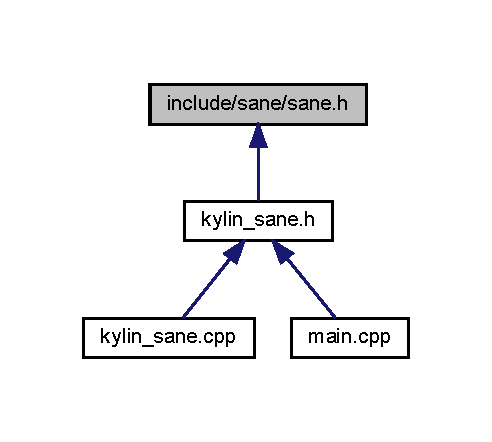
\includegraphics[width=216pt]{sane_8h__dep__incl}
\end{center}
\end{figure}
\doxysubsection*{结构体}
\begin{DoxyCompactItemize}
\item 
struct \mbox{\hyperlink{structSANE__Device}{S\+A\+N\+E\+\_\+\+Device}}
\item 
struct \mbox{\hyperlink{structSANE__Range}{S\+A\+N\+E\+\_\+\+Range}}
\item 
struct \mbox{\hyperlink{structSANE__Option__Descriptor}{S\+A\+N\+E\+\_\+\+Option\+\_\+\+Descriptor}}
\item 
struct \mbox{\hyperlink{structSANE__Parameters}{S\+A\+N\+E\+\_\+\+Parameters}}
\end{DoxyCompactItemize}
\doxysubsection*{宏定义}
\begin{DoxyCompactItemize}
\item 
\#define \mbox{\hyperlink{sane_8h_af62062d17b89208f2362f06597819cdd}{S\+A\+N\+E\+\_\+\+C\+U\+R\+R\+E\+N\+T\+\_\+\+M\+A\+J\+OR}}~1
\item 
\#define \mbox{\hyperlink{sane_8h_af904b0e8c497ffd75ab69842c3ead825}{S\+A\+N\+E\+\_\+\+C\+U\+R\+R\+E\+N\+T\+\_\+\+M\+I\+N\+OR}}~0
\item 
\#define \mbox{\hyperlink{sane_8h_ae46c2944619dc79d653e5ef619105aed}{S\+A\+N\+E\+\_\+\+V\+E\+R\+S\+I\+O\+N\+\_\+\+C\+O\+DE}}(major,  minor,  build)
\item 
\#define \mbox{\hyperlink{sane_8h_a27ef1a3c2953c88b0887708d6ff9cccb}{S\+A\+N\+E\+\_\+\+V\+E\+R\+S\+I\+O\+N\+\_\+\+M\+A\+J\+OR}}(code)~((((\mbox{\hyperlink{sane_8h_aa65d63e57d37984b9d873811a7544b4a}{S\+A\+N\+E\+\_\+\+Word}})(code)) $>$$>$ 24) \&   0xff)
\item 
\#define \mbox{\hyperlink{sane_8h_acdc450ffae31df04ed7274873caed77d}{S\+A\+N\+E\+\_\+\+V\+E\+R\+S\+I\+O\+N\+\_\+\+M\+I\+N\+OR}}(code)~((((\mbox{\hyperlink{sane_8h_aa65d63e57d37984b9d873811a7544b4a}{S\+A\+N\+E\+\_\+\+Word}})(code)) $>$$>$ 16) \&   0xff)
\item 
\#define \mbox{\hyperlink{sane_8h_aa363ddb1b970b05268839aefb8931f0e}{S\+A\+N\+E\+\_\+\+V\+E\+R\+S\+I\+O\+N\+\_\+\+B\+U\+I\+LD}}(code)~((((\mbox{\hyperlink{sane_8h_aa65d63e57d37984b9d873811a7544b4a}{S\+A\+N\+E\+\_\+\+Word}})(code)) $>$$>$  0) \& 0xffff)
\item 
\#define \mbox{\hyperlink{sane_8h_abacc34fe4cf46568bfccadba9c9d8781}{S\+A\+N\+E\+\_\+\+F\+A\+L\+SE}}~0
\item 
\#define \mbox{\hyperlink{sane_8h_af094e0be9cabde26db0fbaedf830077a}{S\+A\+N\+E\+\_\+\+T\+R\+UE}}~1
\item 
\#define \mbox{\hyperlink{sane_8h_aed6bb644c1b084f957114ad852e08c9c}{S\+A\+N\+E\+\_\+\+F\+I\+X\+E\+D\+\_\+\+S\+C\+A\+L\+E\+\_\+\+S\+H\+I\+FT}}~16
\item 
\#define \mbox{\hyperlink{sane_8h_a829f2992b16b123c2200c39968a73d80}{S\+A\+N\+E\+\_\+\+F\+IX}}(v)~((\mbox{\hyperlink{sane_8h_aa65d63e57d37984b9d873811a7544b4a}{S\+A\+N\+E\+\_\+\+Word}}) ((v) $\ast$ (1 $<$$<$ \mbox{\hyperlink{sane_8h_aed6bb644c1b084f957114ad852e08c9c}{S\+A\+N\+E\+\_\+\+F\+I\+X\+E\+D\+\_\+\+S\+C\+A\+L\+E\+\_\+\+S\+H\+I\+FT}})))
\item 
\#define \mbox{\hyperlink{sane_8h_a5c6e54440adafb4789f243e05f9c7cbf}{S\+A\+N\+E\+\_\+\+U\+N\+F\+IX}}(v)~((double)(v) / (1 $<$$<$ \mbox{\hyperlink{sane_8h_aed6bb644c1b084f957114ad852e08c9c}{S\+A\+N\+E\+\_\+\+F\+I\+X\+E\+D\+\_\+\+S\+C\+A\+L\+E\+\_\+\+S\+H\+I\+FT}}))
\item 
\#define \mbox{\hyperlink{sane_8h_add39ed451474e21f8a418bba2dfc13ab}{S\+A\+N\+E\+\_\+\+C\+A\+P\+\_\+\+S\+O\+F\+T\+\_\+\+S\+E\+L\+E\+CT}}~(1 $<$$<$ 0)
\item 
\#define \mbox{\hyperlink{sane_8h_a1d881025e167a2f81a978d0d34be9fb0}{S\+A\+N\+E\+\_\+\+C\+A\+P\+\_\+\+H\+A\+R\+D\+\_\+\+S\+E\+L\+E\+CT}}~(1 $<$$<$ 1)
\item 
\#define \mbox{\hyperlink{sane_8h_ab9b6dcaec64ec76abffc3e6ea1f3253e}{S\+A\+N\+E\+\_\+\+C\+A\+P\+\_\+\+S\+O\+F\+T\+\_\+\+D\+E\+T\+E\+CT}}~(1 $<$$<$ 2)
\item 
\#define \mbox{\hyperlink{sane_8h_a2805bbfe0b2cfe373955bbc18510483d}{S\+A\+N\+E\+\_\+\+C\+A\+P\+\_\+\+E\+M\+U\+L\+A\+T\+ED}}~(1 $<$$<$ 3)
\item 
\#define \mbox{\hyperlink{sane_8h_afd89b61b31442307fb6e0c1a32e53087}{S\+A\+N\+E\+\_\+\+C\+A\+P\+\_\+\+A\+U\+T\+O\+M\+A\+T\+IC}}~(1 $<$$<$ 4)
\item 
\#define \mbox{\hyperlink{sane_8h_a9e7916a94af7f94342c95c7d1e09631c}{S\+A\+N\+E\+\_\+\+C\+A\+P\+\_\+\+I\+N\+A\+C\+T\+I\+VE}}~(1 $<$$<$ 5)
\item 
\#define \mbox{\hyperlink{sane_8h_ae5aa1364e41f98fd14103097e6904885}{S\+A\+N\+E\+\_\+\+C\+A\+P\+\_\+\+A\+D\+V\+A\+N\+C\+ED}}~(1 $<$$<$ 6)
\item 
\#define \mbox{\hyperlink{sane_8h_a06a4546d8670453547a8facaaf00fa12}{S\+A\+N\+E\+\_\+\+O\+P\+T\+I\+O\+N\+\_\+\+I\+S\+\_\+\+A\+C\+T\+I\+VE}}(cap)~(((cap) \& \mbox{\hyperlink{sane_8h_a9e7916a94af7f94342c95c7d1e09631c}{S\+A\+N\+E\+\_\+\+C\+A\+P\+\_\+\+I\+N\+A\+C\+T\+I\+VE}}) == 0)
\item 
\#define \mbox{\hyperlink{sane_8h_a283c9cc564f748cafc4f0d60e24823cb}{S\+A\+N\+E\+\_\+\+O\+P\+T\+I\+O\+N\+\_\+\+I\+S\+\_\+\+S\+E\+T\+T\+A\+B\+LE}}(cap)~(((cap) \& \mbox{\hyperlink{sane_8h_add39ed451474e21f8a418bba2dfc13ab}{S\+A\+N\+E\+\_\+\+C\+A\+P\+\_\+\+S\+O\+F\+T\+\_\+\+S\+E\+L\+E\+CT}}) != 0)
\item 
\#define \mbox{\hyperlink{sane_8h_a2f1730573909a28310318935bd1a296f}{S\+A\+N\+E\+\_\+\+I\+N\+F\+O\+\_\+\+I\+N\+E\+X\+A\+CT}}~(1 $<$$<$ 0)
\item 
\#define \mbox{\hyperlink{sane_8h_a9a34da6251589716a5a1fb7cabbee671}{S\+A\+N\+E\+\_\+\+I\+N\+F\+O\+\_\+\+R\+E\+L\+O\+A\+D\+\_\+\+O\+P\+T\+I\+O\+NS}}~(1 $<$$<$ 1)
\item 
\#define \mbox{\hyperlink{sane_8h_ab0a396e119d4c0671b2548462316dde3}{S\+A\+N\+E\+\_\+\+I\+N\+F\+O\+\_\+\+R\+E\+L\+O\+A\+D\+\_\+\+P\+A\+R\+A\+MS}}~(1 $<$$<$ 2)
\item 
\#define \mbox{\hyperlink{sane_8h_ace070ffd2e0979afdc42eba707117a65}{S\+A\+N\+E\+\_\+\+M\+A\+X\+\_\+\+U\+S\+E\+R\+N\+A\+M\+E\+\_\+\+L\+EN}}~128
\item 
\#define \mbox{\hyperlink{sane_8h_a2e2ef927dbecaadfdd8444a0bbe23eb1}{S\+A\+N\+E\+\_\+\+M\+A\+X\+\_\+\+P\+A\+S\+S\+W\+O\+R\+D\+\_\+\+L\+EN}}~128
\end{DoxyCompactItemize}
\doxysubsection*{类型定义}
\begin{DoxyCompactItemize}
\item 
typedef \mbox{\hyperlink{sane_8h_aa65d63e57d37984b9d873811a7544b4a}{S\+A\+N\+E\+\_\+\+Word}} \mbox{\hyperlink{sane_8h_afb77ef4d4ce97f57e5a9e54393f979ee}{S\+A\+N\+E\+\_\+\+Bool}}
\item 
typedef int \mbox{\hyperlink{sane_8h_aa65d63e57d37984b9d873811a7544b4a}{S\+A\+N\+E\+\_\+\+Word}}
\item 
typedef \mbox{\hyperlink{sane_8h_aa65d63e57d37984b9d873811a7544b4a}{S\+A\+N\+E\+\_\+\+Word}} \mbox{\hyperlink{sane_8h_a18b0de32eae6997909ae9ab0117af3d5}{S\+A\+N\+E\+\_\+\+Int}}
\item 
typedef unsigned char \mbox{\hyperlink{sane_8h_ae81a9c562538e486d29a0e86537763cf}{S\+A\+N\+E\+\_\+\+Byte}}
\item 
typedef char \mbox{\hyperlink{sane_8h_a4e81ae30cff3d1b5781b7adbf684aa52}{S\+A\+N\+E\+\_\+\+Char}}
\item 
typedef \mbox{\hyperlink{sane_8h_a4e81ae30cff3d1b5781b7adbf684aa52}{S\+A\+N\+E\+\_\+\+Char}} $\ast$ \mbox{\hyperlink{sane_8h_a9e545fc1b64c63611113d93dabbc6270}{S\+A\+N\+E\+\_\+\+String}}
\item 
typedef const \mbox{\hyperlink{sane_8h_a4e81ae30cff3d1b5781b7adbf684aa52}{S\+A\+N\+E\+\_\+\+Char}} $\ast$ \mbox{\hyperlink{sane_8h_a9a47323dab2a36db080f1bcc11585af4}{S\+A\+N\+E\+\_\+\+String\+\_\+\+Const}}
\item 
typedef void $\ast$ \mbox{\hyperlink{sane_8h_adff38d40c72e14125709194edfd45e1b}{S\+A\+N\+E\+\_\+\+Handle}}
\item 
typedef \mbox{\hyperlink{sane_8h_aa65d63e57d37984b9d873811a7544b4a}{S\+A\+N\+E\+\_\+\+Word}} \mbox{\hyperlink{sane_8h_ad3262f83c7fec2066a68928be64c5fe6}{S\+A\+N\+E\+\_\+\+Fixed}}
\item 
typedef void($\ast$ \mbox{\hyperlink{sane_8h_a65071043cb6021bddedc7f249d9338ea}{S\+A\+N\+E\+\_\+\+Auth\+\_\+\+Callback}}) (\mbox{\hyperlink{sane_8h_a9a47323dab2a36db080f1bcc11585af4}{S\+A\+N\+E\+\_\+\+String\+\_\+\+Const}} resource, \mbox{\hyperlink{sane_8h_a4e81ae30cff3d1b5781b7adbf684aa52}{S\+A\+N\+E\+\_\+\+Char}} $\ast$username, \mbox{\hyperlink{sane_8h_a4e81ae30cff3d1b5781b7adbf684aa52}{S\+A\+N\+E\+\_\+\+Char}} $\ast$password)
\end{DoxyCompactItemize}
\doxysubsection*{枚举}
\begin{DoxyCompactItemize}
\item 
enum \mbox{\hyperlink{sane_8h_ae5ce8ba47cee42542d1a981be4e4c552}{S\+A\+N\+E\+\_\+\+Status}} \{ \newline
\mbox{\hyperlink{sane_8h_ae5ce8ba47cee42542d1a981be4e4c552a5856c36f7cb46b50a1fcdea81f8b139b}{S\+A\+N\+E\+\_\+\+S\+T\+A\+T\+U\+S\+\_\+\+G\+O\+OD}} = 0, 
\mbox{\hyperlink{sane_8h_ae5ce8ba47cee42542d1a981be4e4c552a9546eafda7b66421f0fe27db97d7464d}{S\+A\+N\+E\+\_\+\+S\+T\+A\+T\+U\+S\+\_\+\+U\+N\+S\+U\+P\+P\+O\+R\+T\+ED}}, 
\mbox{\hyperlink{sane_8h_ae5ce8ba47cee42542d1a981be4e4c552a8b18c5e9a7fd1a9ea6e54a055374efb7}{S\+A\+N\+E\+\_\+\+S\+T\+A\+T\+U\+S\+\_\+\+C\+A\+N\+C\+E\+L\+L\+ED}}, 
\mbox{\hyperlink{sane_8h_ae5ce8ba47cee42542d1a981be4e4c552a45d979d5a8bc43741bd874bf044237ed}{S\+A\+N\+E\+\_\+\+S\+T\+A\+T\+U\+S\+\_\+\+D\+E\+V\+I\+C\+E\+\_\+\+B\+U\+SY}}, 
\newline
\mbox{\hyperlink{sane_8h_ae5ce8ba47cee42542d1a981be4e4c552aa7148d5dbe85059824e9f8110d573131}{S\+A\+N\+E\+\_\+\+S\+T\+A\+T\+U\+S\+\_\+\+I\+N\+V\+AL}}, 
\mbox{\hyperlink{sane_8h_ae5ce8ba47cee42542d1a981be4e4c552af89e9888d716ae6b96adeb66a7a6c07e}{S\+A\+N\+E\+\_\+\+S\+T\+A\+T\+U\+S\+\_\+\+E\+OF}}, 
\mbox{\hyperlink{sane_8h_ae5ce8ba47cee42542d1a981be4e4c552af204f5d74ac5e0af99b03b9de1083f08}{S\+A\+N\+E\+\_\+\+S\+T\+A\+T\+U\+S\+\_\+\+J\+A\+M\+M\+ED}}, 
\mbox{\hyperlink{sane_8h_ae5ce8ba47cee42542d1a981be4e4c552a9ad440fa2a49e318b4a7e30393d25ed4}{S\+A\+N\+E\+\_\+\+S\+T\+A\+T\+U\+S\+\_\+\+N\+O\+\_\+\+D\+O\+CS}}, 
\newline
\mbox{\hyperlink{sane_8h_ae5ce8ba47cee42542d1a981be4e4c552a8e6014f8d917df052fc94a5a7131c8ca}{S\+A\+N\+E\+\_\+\+S\+T\+A\+T\+U\+S\+\_\+\+C\+O\+V\+E\+R\+\_\+\+O\+P\+EN}}, 
\mbox{\hyperlink{sane_8h_ae5ce8ba47cee42542d1a981be4e4c552a72906f90341d8650afd14c1195b21be8}{S\+A\+N\+E\+\_\+\+S\+T\+A\+T\+U\+S\+\_\+\+I\+O\+\_\+\+E\+R\+R\+OR}}, 
\mbox{\hyperlink{sane_8h_ae5ce8ba47cee42542d1a981be4e4c552a882d5c375fb7da926b6789f770af9988}{S\+A\+N\+E\+\_\+\+S\+T\+A\+T\+U\+S\+\_\+\+N\+O\+\_\+\+M\+EM}}, 
\mbox{\hyperlink{sane_8h_ae5ce8ba47cee42542d1a981be4e4c552a58a4769b653ccd02161a02e3114d3dcb}{S\+A\+N\+E\+\_\+\+S\+T\+A\+T\+U\+S\+\_\+\+A\+C\+C\+E\+S\+S\+\_\+\+D\+E\+N\+I\+ED}}
 \}
\item 
enum \mbox{\hyperlink{sane_8h_aed3324dea8f24f5381e12e5562aaf72b}{S\+A\+N\+E\+\_\+\+Value\+\_\+\+Type}} \{ \newline
\mbox{\hyperlink{sane_8h_aed3324dea8f24f5381e12e5562aaf72ba4af54ce4403e7c587775ff842275aa4e}{S\+A\+N\+E\+\_\+\+T\+Y\+P\+E\+\_\+\+B\+O\+OL}} = 0, 
\mbox{\hyperlink{sane_8h_aed3324dea8f24f5381e12e5562aaf72ba3129c48e1653a2d1d5fbf37994eb0d7a}{S\+A\+N\+E\+\_\+\+T\+Y\+P\+E\+\_\+\+I\+NT}}, 
\mbox{\hyperlink{sane_8h_aed3324dea8f24f5381e12e5562aaf72baf533aff76f2b61c9e4464ac50f8b766a}{S\+A\+N\+E\+\_\+\+T\+Y\+P\+E\+\_\+\+F\+I\+X\+ED}}, 
\mbox{\hyperlink{sane_8h_aed3324dea8f24f5381e12e5562aaf72ba498df634f862a8267401634d1728dd3d}{S\+A\+N\+E\+\_\+\+T\+Y\+P\+E\+\_\+\+S\+T\+R\+I\+NG}}, 
\newline
\mbox{\hyperlink{sane_8h_aed3324dea8f24f5381e12e5562aaf72ba547670e294cc09e0ca69014dd4db510a}{S\+A\+N\+E\+\_\+\+T\+Y\+P\+E\+\_\+\+B\+U\+T\+T\+ON}}, 
\mbox{\hyperlink{sane_8h_aed3324dea8f24f5381e12e5562aaf72ba632657c4963a1860dca7d077eac459b9}{S\+A\+N\+E\+\_\+\+T\+Y\+P\+E\+\_\+\+G\+R\+O\+UP}}
 \}
\item 
enum \mbox{\hyperlink{sane_8h_a15e903425f365e0fe30fed1e37446990}{S\+A\+N\+E\+\_\+\+Unit}} \{ \newline
\mbox{\hyperlink{sane_8h_a15e903425f365e0fe30fed1e37446990a08f694989ea5823c2d825f991ad3a468}{S\+A\+N\+E\+\_\+\+U\+N\+I\+T\+\_\+\+N\+O\+NE}} = 0, 
\mbox{\hyperlink{sane_8h_a15e903425f365e0fe30fed1e37446990abe30196cbdfd3f4069e1bf834e933a84}{S\+A\+N\+E\+\_\+\+U\+N\+I\+T\+\_\+\+P\+I\+X\+EL}}, 
\mbox{\hyperlink{sane_8h_a15e903425f365e0fe30fed1e37446990ae551bba514d23aeaf99bed28ae043126}{S\+A\+N\+E\+\_\+\+U\+N\+I\+T\+\_\+\+B\+IT}}, 
\mbox{\hyperlink{sane_8h_a15e903425f365e0fe30fed1e37446990a56751573aa565e0c164cd1ab9fb01996}{S\+A\+N\+E\+\_\+\+U\+N\+I\+T\+\_\+\+MM}}, 
\newline
\mbox{\hyperlink{sane_8h_a15e903425f365e0fe30fed1e37446990a3ee656f5d7afc3be86961859fb0016b8}{S\+A\+N\+E\+\_\+\+U\+N\+I\+T\+\_\+\+D\+PI}}, 
\mbox{\hyperlink{sane_8h_a15e903425f365e0fe30fed1e37446990a5cc13c79bd7cc2baf15c61347458b86e}{S\+A\+N\+E\+\_\+\+U\+N\+I\+T\+\_\+\+P\+E\+R\+C\+E\+NT}}, 
\mbox{\hyperlink{sane_8h_a15e903425f365e0fe30fed1e37446990a5dd9658d2d1a4d907ee326b3e17d1217}{S\+A\+N\+E\+\_\+\+U\+N\+I\+T\+\_\+\+M\+I\+C\+R\+O\+S\+E\+C\+O\+ND}}
 \}
\item 
enum \mbox{\hyperlink{sane_8h_a6422f68f593477ab1fd81078e9afc8e9}{S\+A\+N\+E\+\_\+\+Constraint\+\_\+\+Type}} \{ \mbox{\hyperlink{sane_8h_a6422f68f593477ab1fd81078e9afc8e9aa241b482716bc33d0e9cf8b13a5c5af7}{S\+A\+N\+E\+\_\+\+C\+O\+N\+S\+T\+R\+A\+I\+N\+T\+\_\+\+N\+O\+NE}} = 0, 
\mbox{\hyperlink{sane_8h_a6422f68f593477ab1fd81078e9afc8e9a2c5b18bc1b10dcb8449651777a858871}{S\+A\+N\+E\+\_\+\+C\+O\+N\+S\+T\+R\+A\+I\+N\+T\+\_\+\+R\+A\+N\+GE}}, 
\mbox{\hyperlink{sane_8h_a6422f68f593477ab1fd81078e9afc8e9abd1ba1f152d79a2767dc16dd50e28732}{S\+A\+N\+E\+\_\+\+C\+O\+N\+S\+T\+R\+A\+I\+N\+T\+\_\+\+W\+O\+R\+D\+\_\+\+L\+I\+ST}}, 
\mbox{\hyperlink{sane_8h_a6422f68f593477ab1fd81078e9afc8e9afce2c30a30f6acf78bbf31fdd3c0300d}{S\+A\+N\+E\+\_\+\+C\+O\+N\+S\+T\+R\+A\+I\+N\+T\+\_\+\+S\+T\+R\+I\+N\+G\+\_\+\+L\+I\+ST}}
 \}
\item 
enum \mbox{\hyperlink{sane_8h_a676e37749b97063237ac22f5d8ae7cd7}{S\+A\+N\+E\+\_\+\+Action}} \{ \mbox{\hyperlink{sane_8h_a676e37749b97063237ac22f5d8ae7cd7a159621772b084fae63cb8a6e9a7232f0}{S\+A\+N\+E\+\_\+\+A\+C\+T\+I\+O\+N\+\_\+\+G\+E\+T\+\_\+\+V\+A\+L\+UE}} = 0, 
\mbox{\hyperlink{sane_8h_a676e37749b97063237ac22f5d8ae7cd7a9e38f6099fff31b864ca76a362f7c121}{S\+A\+N\+E\+\_\+\+A\+C\+T\+I\+O\+N\+\_\+\+S\+E\+T\+\_\+\+V\+A\+L\+UE}}, 
\mbox{\hyperlink{sane_8h_a676e37749b97063237ac22f5d8ae7cd7ac95cf0bff7559e19f56c06fb2447433e}{S\+A\+N\+E\+\_\+\+A\+C\+T\+I\+O\+N\+\_\+\+S\+E\+T\+\_\+\+A\+U\+TO}}
 \}
\item 
enum \mbox{\hyperlink{sane_8h_ac5182b25bf83c5e16c4e6e8d998eecac}{S\+A\+N\+E\+\_\+\+Frame}} \{ \newline
\mbox{\hyperlink{sane_8h_ac5182b25bf83c5e16c4e6e8d998eecaca714285a130698b64e654b0b7084d4869}{S\+A\+N\+E\+\_\+\+F\+R\+A\+M\+E\+\_\+\+G\+R\+AY}}, 
\mbox{\hyperlink{sane_8h_ac5182b25bf83c5e16c4e6e8d998eecaca02f8e814fea4e3f8a577579b96feb27b}{S\+A\+N\+E\+\_\+\+F\+R\+A\+M\+E\+\_\+\+R\+GB}}, 
\mbox{\hyperlink{sane_8h_ac5182b25bf83c5e16c4e6e8d998eecacabedeb0627576b57ad708c3590600195d}{S\+A\+N\+E\+\_\+\+F\+R\+A\+M\+E\+\_\+\+R\+ED}}, 
\mbox{\hyperlink{sane_8h_ac5182b25bf83c5e16c4e6e8d998eecaca69cb439dedf5db3fd5b54e4903c526e6}{S\+A\+N\+E\+\_\+\+F\+R\+A\+M\+E\+\_\+\+G\+R\+E\+EN}}, 
\newline
\mbox{\hyperlink{sane_8h_ac5182b25bf83c5e16c4e6e8d998eecaca14d6443493d7e3e9e1d4761c170dc3d7}{S\+A\+N\+E\+\_\+\+F\+R\+A\+M\+E\+\_\+\+B\+L\+UE}}
 \}
\end{DoxyCompactItemize}
\doxysubsection*{函数}
\begin{DoxyCompactItemize}
\item 
\mbox{\hyperlink{sane_8h_ae5ce8ba47cee42542d1a981be4e4c552}{S\+A\+N\+E\+\_\+\+Status}} \mbox{\hyperlink{sane_8h_a1498918f9c7e543a4a757482bcffd7a9}{sane\+\_\+init}} (\mbox{\hyperlink{sane_8h_a18b0de32eae6997909ae9ab0117af3d5}{S\+A\+N\+E\+\_\+\+Int}} $\ast$version\+\_\+code, \mbox{\hyperlink{sane_8h_a65071043cb6021bddedc7f249d9338ea}{S\+A\+N\+E\+\_\+\+Auth\+\_\+\+Callback}} authorize)
\item 
void \mbox{\hyperlink{sane_8h_adee134f0b60b099d3ddb144ec7266c6a}{sane\+\_\+exit}} (void)
\begin{DoxyCompactList}\small\item\em 退出后端 \end{DoxyCompactList}\item 
\mbox{\hyperlink{sane_8h_ae5ce8ba47cee42542d1a981be4e4c552}{S\+A\+N\+E\+\_\+\+Status}} \mbox{\hyperlink{sane_8h_a86a720cead710936ba84b6de59b16623}{sane\+\_\+get\+\_\+devices}} (const \mbox{\hyperlink{structSANE__Device}{S\+A\+N\+E\+\_\+\+Device}} $\ast$$\ast$$\ast$device\+\_\+list, \mbox{\hyperlink{sane_8h_afb77ef4d4ce97f57e5a9e54393f979ee}{S\+A\+N\+E\+\_\+\+Bool}} local\+\_\+only)
\item 
\mbox{\hyperlink{sane_8h_ae5ce8ba47cee42542d1a981be4e4c552}{S\+A\+N\+E\+\_\+\+Status}} \mbox{\hyperlink{sane_8h_adfeda33e4d60e0d6a4e19634cc9c2bae}{sane\+\_\+open}} (\mbox{\hyperlink{sane_8h_a9a47323dab2a36db080f1bcc11585af4}{S\+A\+N\+E\+\_\+\+String\+\_\+\+Const}} devicename, \mbox{\hyperlink{sane_8h_adff38d40c72e14125709194edfd45e1b}{S\+A\+N\+E\+\_\+\+Handle}} $\ast$handle)
\item 
void \mbox{\hyperlink{sane_8h_a86bc6c8bf32a9e1ab2dc681dcf8489f1}{sane\+\_\+close}} (\mbox{\hyperlink{sane_8h_adff38d40c72e14125709194edfd45e1b}{S\+A\+N\+E\+\_\+\+Handle}} handle)
\item 
const \mbox{\hyperlink{structSANE__Option__Descriptor}{S\+A\+N\+E\+\_\+\+Option\+\_\+\+Descriptor}} $\ast$ \mbox{\hyperlink{sane_8h_a7728e01a38c5e18385e383a6ce4a108d}{sane\+\_\+get\+\_\+option\+\_\+descriptor}} (\mbox{\hyperlink{sane_8h_adff38d40c72e14125709194edfd45e1b}{S\+A\+N\+E\+\_\+\+Handle}} handle, \mbox{\hyperlink{sane_8h_a18b0de32eae6997909ae9ab0117af3d5}{S\+A\+N\+E\+\_\+\+Int}} option)
\item 
\mbox{\hyperlink{sane_8h_ae5ce8ba47cee42542d1a981be4e4c552}{S\+A\+N\+E\+\_\+\+Status}} \mbox{\hyperlink{sane_8h_af97b5a648c359cdeb17844f24e74f21d}{sane\+\_\+control\+\_\+option}} (\mbox{\hyperlink{sane_8h_adff38d40c72e14125709194edfd45e1b}{S\+A\+N\+E\+\_\+\+Handle}} handle, \mbox{\hyperlink{sane_8h_a18b0de32eae6997909ae9ab0117af3d5}{S\+A\+N\+E\+\_\+\+Int}} option, \mbox{\hyperlink{sane_8h_a676e37749b97063237ac22f5d8ae7cd7}{S\+A\+N\+E\+\_\+\+Action}} action, void $\ast$value, \mbox{\hyperlink{sane_8h_a18b0de32eae6997909ae9ab0117af3d5}{S\+A\+N\+E\+\_\+\+Int}} $\ast$info)
\item 
\mbox{\hyperlink{sane_8h_ae5ce8ba47cee42542d1a981be4e4c552}{S\+A\+N\+E\+\_\+\+Status}} \mbox{\hyperlink{sane_8h_a28ba54307cb61e48fc1a361be7ad2c6e}{sane\+\_\+get\+\_\+parameters}} (\mbox{\hyperlink{sane_8h_adff38d40c72e14125709194edfd45e1b}{S\+A\+N\+E\+\_\+\+Handle}} handle, \mbox{\hyperlink{structSANE__Parameters}{S\+A\+N\+E\+\_\+\+Parameters}} $\ast$params)
\item 
\mbox{\hyperlink{sane_8h_ae5ce8ba47cee42542d1a981be4e4c552}{S\+A\+N\+E\+\_\+\+Status}} \mbox{\hyperlink{sane_8h_a633f90b105f09ca798ecbf9a77711e7b}{sane\+\_\+start}} (\mbox{\hyperlink{sane_8h_adff38d40c72e14125709194edfd45e1b}{S\+A\+N\+E\+\_\+\+Handle}} handle)
\item 
\mbox{\hyperlink{sane_8h_ae5ce8ba47cee42542d1a981be4e4c552}{S\+A\+N\+E\+\_\+\+Status}} \mbox{\hyperlink{sane_8h_ae5426bddf1bfe3d30370c9fe2d209cc3}{sane\+\_\+read}} (\mbox{\hyperlink{sane_8h_adff38d40c72e14125709194edfd45e1b}{S\+A\+N\+E\+\_\+\+Handle}} handle, \mbox{\hyperlink{sane_8h_ae81a9c562538e486d29a0e86537763cf}{S\+A\+N\+E\+\_\+\+Byte}} $\ast$data, \mbox{\hyperlink{sane_8h_a18b0de32eae6997909ae9ab0117af3d5}{S\+A\+N\+E\+\_\+\+Int}} max\+\_\+length, \mbox{\hyperlink{sane_8h_a18b0de32eae6997909ae9ab0117af3d5}{S\+A\+N\+E\+\_\+\+Int}} $\ast$length)
\item 
void \mbox{\hyperlink{sane_8h_a8facc0281b730ce19e17971e5c042de1}{sane\+\_\+cancel}} (\mbox{\hyperlink{sane_8h_adff38d40c72e14125709194edfd45e1b}{S\+A\+N\+E\+\_\+\+Handle}} handle)
\item 
\mbox{\hyperlink{sane_8h_ae5ce8ba47cee42542d1a981be4e4c552}{S\+A\+N\+E\+\_\+\+Status}} \mbox{\hyperlink{sane_8h_a1ee82e5f0a83ca9c96c17dbbba7cf543}{sane\+\_\+set\+\_\+io\+\_\+mode}} (\mbox{\hyperlink{sane_8h_adff38d40c72e14125709194edfd45e1b}{S\+A\+N\+E\+\_\+\+Handle}} handle, \mbox{\hyperlink{sane_8h_afb77ef4d4ce97f57e5a9e54393f979ee}{S\+A\+N\+E\+\_\+\+Bool}} non\+\_\+blocking)
\item 
\mbox{\hyperlink{sane_8h_ae5ce8ba47cee42542d1a981be4e4c552}{S\+A\+N\+E\+\_\+\+Status}} \mbox{\hyperlink{sane_8h_a6699a6bb08baa461b98d62fcdd82d8d4}{sane\+\_\+get\+\_\+select\+\_\+fd}} (\mbox{\hyperlink{sane_8h_adff38d40c72e14125709194edfd45e1b}{S\+A\+N\+E\+\_\+\+Handle}} handle, \mbox{\hyperlink{sane_8h_a18b0de32eae6997909ae9ab0117af3d5}{S\+A\+N\+E\+\_\+\+Int}} $\ast$fd)
\item 
\mbox{\hyperlink{sane_8h_a9a47323dab2a36db080f1bcc11585af4}{S\+A\+N\+E\+\_\+\+String\+\_\+\+Const}} \mbox{\hyperlink{sane_8h_a005fc36c746f3b57fcf8108435f0684d}{sane\+\_\+strstatus}} (\mbox{\hyperlink{sane_8h_ae5ce8ba47cee42542d1a981be4e4c552}{S\+A\+N\+E\+\_\+\+Status}} status)
\end{DoxyCompactItemize}


\doxysubsection{详细描述}
\mbox{\hyperlink{sane_8h}{sane.\+h}} A\+P\+I规范文档 

\begin{DoxyAuthor}{作者}
yusq 
\end{DoxyAuthor}
\begin{DoxyDate}{日期}
2020年 03月 13日 星期五 17\+:28\+:03 C\+ST
\end{DoxyDate}
sane A\+P\+I接口文档用于扫描软件的研发 

\doxysubsection{宏定义说明}
\mbox{\Hypertarget{sane_8h_ae5aa1364e41f98fd14103097e6904885}\label{sane_8h_ae5aa1364e41f98fd14103097e6904885}} 
\index{sane.h@{sane.h}!SANE\_CAP\_ADVANCED@{SANE\_CAP\_ADVANCED}}
\index{SANE\_CAP\_ADVANCED@{SANE\_CAP\_ADVANCED}!sane.h@{sane.h}}
\doxysubsubsection{\texorpdfstring{SANE\_CAP\_ADVANCED}{SANE\_CAP\_ADVANCED}}
{\footnotesize\ttfamily \#define S\+A\+N\+E\+\_\+\+C\+A\+P\+\_\+\+A\+D\+V\+A\+N\+C\+ED~(1 $<$$<$ 6)}

\mbox{\Hypertarget{sane_8h_afd89b61b31442307fb6e0c1a32e53087}\label{sane_8h_afd89b61b31442307fb6e0c1a32e53087}} 
\index{sane.h@{sane.h}!SANE\_CAP\_AUTOMATIC@{SANE\_CAP\_AUTOMATIC}}
\index{SANE\_CAP\_AUTOMATIC@{SANE\_CAP\_AUTOMATIC}!sane.h@{sane.h}}
\doxysubsubsection{\texorpdfstring{SANE\_CAP\_AUTOMATIC}{SANE\_CAP\_AUTOMATIC}}
{\footnotesize\ttfamily \#define S\+A\+N\+E\+\_\+\+C\+A\+P\+\_\+\+A\+U\+T\+O\+M\+A\+T\+IC~(1 $<$$<$ 4)}

\mbox{\Hypertarget{sane_8h_a2805bbfe0b2cfe373955bbc18510483d}\label{sane_8h_a2805bbfe0b2cfe373955bbc18510483d}} 
\index{sane.h@{sane.h}!SANE\_CAP\_EMULATED@{SANE\_CAP\_EMULATED}}
\index{SANE\_CAP\_EMULATED@{SANE\_CAP\_EMULATED}!sane.h@{sane.h}}
\doxysubsubsection{\texorpdfstring{SANE\_CAP\_EMULATED}{SANE\_CAP\_EMULATED}}
{\footnotesize\ttfamily \#define S\+A\+N\+E\+\_\+\+C\+A\+P\+\_\+\+E\+M\+U\+L\+A\+T\+ED~(1 $<$$<$ 3)}

\mbox{\Hypertarget{sane_8h_a1d881025e167a2f81a978d0d34be9fb0}\label{sane_8h_a1d881025e167a2f81a978d0d34be9fb0}} 
\index{sane.h@{sane.h}!SANE\_CAP\_HARD\_SELECT@{SANE\_CAP\_HARD\_SELECT}}
\index{SANE\_CAP\_HARD\_SELECT@{SANE\_CAP\_HARD\_SELECT}!sane.h@{sane.h}}
\doxysubsubsection{\texorpdfstring{SANE\_CAP\_HARD\_SELECT}{SANE\_CAP\_HARD\_SELECT}}
{\footnotesize\ttfamily \#define S\+A\+N\+E\+\_\+\+C\+A\+P\+\_\+\+H\+A\+R\+D\+\_\+\+S\+E\+L\+E\+CT~(1 $<$$<$ 1)}

\mbox{\Hypertarget{sane_8h_a9e7916a94af7f94342c95c7d1e09631c}\label{sane_8h_a9e7916a94af7f94342c95c7d1e09631c}} 
\index{sane.h@{sane.h}!SANE\_CAP\_INACTIVE@{SANE\_CAP\_INACTIVE}}
\index{SANE\_CAP\_INACTIVE@{SANE\_CAP\_INACTIVE}!sane.h@{sane.h}}
\doxysubsubsection{\texorpdfstring{SANE\_CAP\_INACTIVE}{SANE\_CAP\_INACTIVE}}
{\footnotesize\ttfamily \#define S\+A\+N\+E\+\_\+\+C\+A\+P\+\_\+\+I\+N\+A\+C\+T\+I\+VE~(1 $<$$<$ 5)}

\mbox{\Hypertarget{sane_8h_ab9b6dcaec64ec76abffc3e6ea1f3253e}\label{sane_8h_ab9b6dcaec64ec76abffc3e6ea1f3253e}} 
\index{sane.h@{sane.h}!SANE\_CAP\_SOFT\_DETECT@{SANE\_CAP\_SOFT\_DETECT}}
\index{SANE\_CAP\_SOFT\_DETECT@{SANE\_CAP\_SOFT\_DETECT}!sane.h@{sane.h}}
\doxysubsubsection{\texorpdfstring{SANE\_CAP\_SOFT\_DETECT}{SANE\_CAP\_SOFT\_DETECT}}
{\footnotesize\ttfamily \#define S\+A\+N\+E\+\_\+\+C\+A\+P\+\_\+\+S\+O\+F\+T\+\_\+\+D\+E\+T\+E\+CT~(1 $<$$<$ 2)}

\mbox{\Hypertarget{sane_8h_add39ed451474e21f8a418bba2dfc13ab}\label{sane_8h_add39ed451474e21f8a418bba2dfc13ab}} 
\index{sane.h@{sane.h}!SANE\_CAP\_SOFT\_SELECT@{SANE\_CAP\_SOFT\_SELECT}}
\index{SANE\_CAP\_SOFT\_SELECT@{SANE\_CAP\_SOFT\_SELECT}!sane.h@{sane.h}}
\doxysubsubsection{\texorpdfstring{SANE\_CAP\_SOFT\_SELECT}{SANE\_CAP\_SOFT\_SELECT}}
{\footnotesize\ttfamily \#define S\+A\+N\+E\+\_\+\+C\+A\+P\+\_\+\+S\+O\+F\+T\+\_\+\+S\+E\+L\+E\+CT~(1 $<$$<$ 0)}

\mbox{\Hypertarget{sane_8h_af62062d17b89208f2362f06597819cdd}\label{sane_8h_af62062d17b89208f2362f06597819cdd}} 
\index{sane.h@{sane.h}!SANE\_CURRENT\_MAJOR@{SANE\_CURRENT\_MAJOR}}
\index{SANE\_CURRENT\_MAJOR@{SANE\_CURRENT\_MAJOR}!sane.h@{sane.h}}
\doxysubsubsection{\texorpdfstring{SANE\_CURRENT\_MAJOR}{SANE\_CURRENT\_MAJOR}}
{\footnotesize\ttfamily \#define S\+A\+N\+E\+\_\+\+C\+U\+R\+R\+E\+N\+T\+\_\+\+M\+A\+J\+OR~1}

S\+A\+NE types and defines \mbox{\Hypertarget{sane_8h_af904b0e8c497ffd75ab69842c3ead825}\label{sane_8h_af904b0e8c497ffd75ab69842c3ead825}} 
\index{sane.h@{sane.h}!SANE\_CURRENT\_MINOR@{SANE\_CURRENT\_MINOR}}
\index{SANE\_CURRENT\_MINOR@{SANE\_CURRENT\_MINOR}!sane.h@{sane.h}}
\doxysubsubsection{\texorpdfstring{SANE\_CURRENT\_MINOR}{SANE\_CURRENT\_MINOR}}
{\footnotesize\ttfamily \#define S\+A\+N\+E\+\_\+\+C\+U\+R\+R\+E\+N\+T\+\_\+\+M\+I\+N\+OR~0}

\mbox{\Hypertarget{sane_8h_abacc34fe4cf46568bfccadba9c9d8781}\label{sane_8h_abacc34fe4cf46568bfccadba9c9d8781}} 
\index{sane.h@{sane.h}!SANE\_FALSE@{SANE\_FALSE}}
\index{SANE\_FALSE@{SANE\_FALSE}!sane.h@{sane.h}}
\doxysubsubsection{\texorpdfstring{SANE\_FALSE}{SANE\_FALSE}}
{\footnotesize\ttfamily \#define S\+A\+N\+E\+\_\+\+F\+A\+L\+SE~0}

\mbox{\Hypertarget{sane_8h_a829f2992b16b123c2200c39968a73d80}\label{sane_8h_a829f2992b16b123c2200c39968a73d80}} 
\index{sane.h@{sane.h}!SANE\_FIX@{SANE\_FIX}}
\index{SANE\_FIX@{SANE\_FIX}!sane.h@{sane.h}}
\doxysubsubsection{\texorpdfstring{SANE\_FIX}{SANE\_FIX}}
{\footnotesize\ttfamily \#define S\+A\+N\+E\+\_\+\+F\+IX(\begin{DoxyParamCaption}\item[{}]{v }\end{DoxyParamCaption})~((\mbox{\hyperlink{sane_8h_aa65d63e57d37984b9d873811a7544b4a}{S\+A\+N\+E\+\_\+\+Word}}) ((v) $\ast$ (1 $<$$<$ \mbox{\hyperlink{sane_8h_aed6bb644c1b084f957114ad852e08c9c}{S\+A\+N\+E\+\_\+\+F\+I\+X\+E\+D\+\_\+\+S\+C\+A\+L\+E\+\_\+\+S\+H\+I\+FT}})))}

并没有要求在以下两个表达式保持为真(即使值w $^\wedge$和d在范围内): S\+A\+N\+E\+\_\+\+U\+N\+F\+I\+X(\+S\+A\+N\+E\+\_\+\+F\+I\+X(d))== d S\+A\+N\+E\+\_\+\+F\+I\+X(\+S\+A\+N\+E\+\_\+\+U\+N\+F\+I\+X(w))== w 换句话说,固定值和双精度值之间的转换可能是有损的。因此,建议避免在两种表示形式之间重复转换。 \mbox{\Hypertarget{sane_8h_aed6bb644c1b084f957114ad852e08c9c}\label{sane_8h_aed6bb644c1b084f957114ad852e08c9c}} 
\index{sane.h@{sane.h}!SANE\_FIXED\_SCALE\_SHIFT@{SANE\_FIXED\_SCALE\_SHIFT}}
\index{SANE\_FIXED\_SCALE\_SHIFT@{SANE\_FIXED\_SCALE\_SHIFT}!sane.h@{sane.h}}
\doxysubsubsection{\texorpdfstring{SANE\_FIXED\_SCALE\_SHIFT}{SANE\_FIXED\_SCALE\_SHIFT}}
{\footnotesize\ttfamily \#define S\+A\+N\+E\+\_\+\+F\+I\+X\+E\+D\+\_\+\+S\+C\+A\+L\+E\+\_\+\+S\+H\+I\+FT~16}

定点类型 用于变量,定点值可以在-\/32768到32767.9999之间,分辨率为1/65535 宏\+S\+A\+N\+E\+\_\+\+F\+I\+X\+E\+D\+\_\+\+S\+C\+A\+L\+E\+\_\+\+S\+H\+I\+F\+T给出固定二进制点的位置。该标准将该值定义为16,从而产生1/65536的分辨率。 \mbox{\Hypertarget{sane_8h_a2f1730573909a28310318935bd1a296f}\label{sane_8h_a2f1730573909a28310318935bd1a296f}} 
\index{sane.h@{sane.h}!SANE\_INFO\_INEXACT@{SANE\_INFO\_INEXACT}}
\index{SANE\_INFO\_INEXACT@{SANE\_INFO\_INEXACT}!sane.h@{sane.h}}
\doxysubsubsection{\texorpdfstring{SANE\_INFO\_INEXACT}{SANE\_INFO\_INEXACT}}
{\footnotesize\ttfamily \#define S\+A\+N\+E\+\_\+\+I\+N\+F\+O\+\_\+\+I\+N\+E\+X\+A\+CT~(1 $<$$<$ 0)}

\mbox{\Hypertarget{sane_8h_a9a34da6251589716a5a1fb7cabbee671}\label{sane_8h_a9a34da6251589716a5a1fb7cabbee671}} 
\index{sane.h@{sane.h}!SANE\_INFO\_RELOAD\_OPTIONS@{SANE\_INFO\_RELOAD\_OPTIONS}}
\index{SANE\_INFO\_RELOAD\_OPTIONS@{SANE\_INFO\_RELOAD\_OPTIONS}!sane.h@{sane.h}}
\doxysubsubsection{\texorpdfstring{SANE\_INFO\_RELOAD\_OPTIONS}{SANE\_INFO\_RELOAD\_OPTIONS}}
{\footnotesize\ttfamily \#define S\+A\+N\+E\+\_\+\+I\+N\+F\+O\+\_\+\+R\+E\+L\+O\+A\+D\+\_\+\+O\+P\+T\+I\+O\+NS~(1 $<$$<$ 1)}

\mbox{\Hypertarget{sane_8h_ab0a396e119d4c0671b2548462316dde3}\label{sane_8h_ab0a396e119d4c0671b2548462316dde3}} 
\index{sane.h@{sane.h}!SANE\_INFO\_RELOAD\_PARAMS@{SANE\_INFO\_RELOAD\_PARAMS}}
\index{SANE\_INFO\_RELOAD\_PARAMS@{SANE\_INFO\_RELOAD\_PARAMS}!sane.h@{sane.h}}
\doxysubsubsection{\texorpdfstring{SANE\_INFO\_RELOAD\_PARAMS}{SANE\_INFO\_RELOAD\_PARAMS}}
{\footnotesize\ttfamily \#define S\+A\+N\+E\+\_\+\+I\+N\+F\+O\+\_\+\+R\+E\+L\+O\+A\+D\+\_\+\+P\+A\+R\+A\+MS~(1 $<$$<$ 2)}

\mbox{\Hypertarget{sane_8h_a2e2ef927dbecaadfdd8444a0bbe23eb1}\label{sane_8h_a2e2ef927dbecaadfdd8444a0bbe23eb1}} 
\index{sane.h@{sane.h}!SANE\_MAX\_PASSWORD\_LEN@{SANE\_MAX\_PASSWORD\_LEN}}
\index{SANE\_MAX\_PASSWORD\_LEN@{SANE\_MAX\_PASSWORD\_LEN}!sane.h@{sane.h}}
\doxysubsubsection{\texorpdfstring{SANE\_MAX\_PASSWORD\_LEN}{SANE\_MAX\_PASSWORD\_LEN}}
{\footnotesize\ttfamily \#define S\+A\+N\+E\+\_\+\+M\+A\+X\+\_\+\+P\+A\+S\+S\+W\+O\+R\+D\+\_\+\+L\+EN~128}

\mbox{\Hypertarget{sane_8h_ace070ffd2e0979afdc42eba707117a65}\label{sane_8h_ace070ffd2e0979afdc42eba707117a65}} 
\index{sane.h@{sane.h}!SANE\_MAX\_USERNAME\_LEN@{SANE\_MAX\_USERNAME\_LEN}}
\index{SANE\_MAX\_USERNAME\_LEN@{SANE\_MAX\_USERNAME\_LEN}!sane.h@{sane.h}}
\doxysubsubsection{\texorpdfstring{SANE\_MAX\_USERNAME\_LEN}{SANE\_MAX\_USERNAME\_LEN}}
{\footnotesize\ttfamily \#define S\+A\+N\+E\+\_\+\+M\+A\+X\+\_\+\+U\+S\+E\+R\+N\+A\+M\+E\+\_\+\+L\+EN~128}

\mbox{\Hypertarget{sane_8h_a06a4546d8670453547a8facaaf00fa12}\label{sane_8h_a06a4546d8670453547a8facaaf00fa12}} 
\index{sane.h@{sane.h}!SANE\_OPTION\_IS\_ACTIVE@{SANE\_OPTION\_IS\_ACTIVE}}
\index{SANE\_OPTION\_IS\_ACTIVE@{SANE\_OPTION\_IS\_ACTIVE}!sane.h@{sane.h}}
\doxysubsubsection{\texorpdfstring{SANE\_OPTION\_IS\_ACTIVE}{SANE\_OPTION\_IS\_ACTIVE}}
{\footnotesize\ttfamily \#define S\+A\+N\+E\+\_\+\+O\+P\+T\+I\+O\+N\+\_\+\+I\+S\+\_\+\+A\+C\+T\+I\+VE(\begin{DoxyParamCaption}\item[{}]{cap }\end{DoxyParamCaption})~(((cap) \& \mbox{\hyperlink{sane_8h_a9e7916a94af7f94342c95c7d1e09631c}{S\+A\+N\+E\+\_\+\+C\+A\+P\+\_\+\+I\+N\+A\+C\+T\+I\+VE}}) == 0)}

\mbox{\Hypertarget{sane_8h_a283c9cc564f748cafc4f0d60e24823cb}\label{sane_8h_a283c9cc564f748cafc4f0d60e24823cb}} 
\index{sane.h@{sane.h}!SANE\_OPTION\_IS\_SETTABLE@{SANE\_OPTION\_IS\_SETTABLE}}
\index{SANE\_OPTION\_IS\_SETTABLE@{SANE\_OPTION\_IS\_SETTABLE}!sane.h@{sane.h}}
\doxysubsubsection{\texorpdfstring{SANE\_OPTION\_IS\_SETTABLE}{SANE\_OPTION\_IS\_SETTABLE}}
{\footnotesize\ttfamily \#define S\+A\+N\+E\+\_\+\+O\+P\+T\+I\+O\+N\+\_\+\+I\+S\+\_\+\+S\+E\+T\+T\+A\+B\+LE(\begin{DoxyParamCaption}\item[{}]{cap }\end{DoxyParamCaption})~(((cap) \& \mbox{\hyperlink{sane_8h_add39ed451474e21f8a418bba2dfc13ab}{S\+A\+N\+E\+\_\+\+C\+A\+P\+\_\+\+S\+O\+F\+T\+\_\+\+S\+E\+L\+E\+CT}}) != 0)}

\mbox{\Hypertarget{sane_8h_af094e0be9cabde26db0fbaedf830077a}\label{sane_8h_af094e0be9cabde26db0fbaedf830077a}} 
\index{sane.h@{sane.h}!SANE\_TRUE@{SANE\_TRUE}}
\index{SANE\_TRUE@{SANE\_TRUE}!sane.h@{sane.h}}
\doxysubsubsection{\texorpdfstring{SANE\_TRUE}{SANE\_TRUE}}
{\footnotesize\ttfamily \#define S\+A\+N\+E\+\_\+\+T\+R\+UE~1}

\mbox{\Hypertarget{sane_8h_a5c6e54440adafb4789f243e05f9c7cbf}\label{sane_8h_a5c6e54440adafb4789f243e05f9c7cbf}} 
\index{sane.h@{sane.h}!SANE\_UNFIX@{SANE\_UNFIX}}
\index{SANE\_UNFIX@{SANE\_UNFIX}!sane.h@{sane.h}}
\doxysubsubsection{\texorpdfstring{SANE\_UNFIX}{SANE\_UNFIX}}
{\footnotesize\ttfamily \#define S\+A\+N\+E\+\_\+\+U\+N\+F\+IX(\begin{DoxyParamCaption}\item[{}]{v }\end{DoxyParamCaption})~((double)(v) / (1 $<$$<$ \mbox{\hyperlink{sane_8h_aed6bb644c1b084f957114ad852e08c9c}{S\+A\+N\+E\+\_\+\+F\+I\+X\+E\+D\+\_\+\+S\+C\+A\+L\+E\+\_\+\+S\+H\+I\+FT}}))}

\mbox{\Hypertarget{sane_8h_aa363ddb1b970b05268839aefb8931f0e}\label{sane_8h_aa363ddb1b970b05268839aefb8931f0e}} 
\index{sane.h@{sane.h}!SANE\_VERSION\_BUILD@{SANE\_VERSION\_BUILD}}
\index{SANE\_VERSION\_BUILD@{SANE\_VERSION\_BUILD}!sane.h@{sane.h}}
\doxysubsubsection{\texorpdfstring{SANE\_VERSION\_BUILD}{SANE\_VERSION\_BUILD}}
{\footnotesize\ttfamily \#define S\+A\+N\+E\+\_\+\+V\+E\+R\+S\+I\+O\+N\+\_\+\+B\+U\+I\+LD(\begin{DoxyParamCaption}\item[{}]{code }\end{DoxyParamCaption})~((((\mbox{\hyperlink{sane_8h_aa65d63e57d37984b9d873811a7544b4a}{S\+A\+N\+E\+\_\+\+Word}})(code)) $>$$>$  0) \& 0xffff)}

\mbox{\Hypertarget{sane_8h_ae46c2944619dc79d653e5ef619105aed}\label{sane_8h_ae46c2944619dc79d653e5ef619105aed}} 
\index{sane.h@{sane.h}!SANE\_VERSION\_CODE@{SANE\_VERSION\_CODE}}
\index{SANE\_VERSION\_CODE@{SANE\_VERSION\_CODE}!sane.h@{sane.h}}
\doxysubsubsection{\texorpdfstring{SANE\_VERSION\_CODE}{SANE\_VERSION\_CODE}}
{\footnotesize\ttfamily \#define S\+A\+N\+E\+\_\+\+V\+E\+R\+S\+I\+O\+N\+\_\+\+C\+O\+DE(\begin{DoxyParamCaption}\item[{}]{major,  }\item[{}]{minor,  }\item[{}]{build }\end{DoxyParamCaption})}

{\bfseries 值\+:}
\begin{DoxyCode}{0}
\DoxyCodeLine{  (  (((\mbox{\hyperlink{sane_8h_aa65d63e57d37984b9d873811a7544b4a}{SANE\_Word}}) (major) \&   0xff) << 24)    \(\backslash\)}
\DoxyCodeLine{   | (((\mbox{\hyperlink{sane_8h_aa65d63e57d37984b9d873811a7544b4a}{SANE\_Word}}) (minor) \&   0xff) << 16)    \(\backslash\)}
\DoxyCodeLine{   | (((\mbox{\hyperlink{sane_8h_aa65d63e57d37984b9d873811a7544b4a}{SANE\_Word}}) (build) \& 0xffff) <<  0))}

\end{DoxyCode}
\mbox{\Hypertarget{sane_8h_a27ef1a3c2953c88b0887708d6ff9cccb}\label{sane_8h_a27ef1a3c2953c88b0887708d6ff9cccb}} 
\index{sane.h@{sane.h}!SANE\_VERSION\_MAJOR@{SANE\_VERSION\_MAJOR}}
\index{SANE\_VERSION\_MAJOR@{SANE\_VERSION\_MAJOR}!sane.h@{sane.h}}
\doxysubsubsection{\texorpdfstring{SANE\_VERSION\_MAJOR}{SANE\_VERSION\_MAJOR}}
{\footnotesize\ttfamily \#define S\+A\+N\+E\+\_\+\+V\+E\+R\+S\+I\+O\+N\+\_\+\+M\+A\+J\+OR(\begin{DoxyParamCaption}\item[{}]{code }\end{DoxyParamCaption})~((((\mbox{\hyperlink{sane_8h_aa65d63e57d37984b9d873811a7544b4a}{S\+A\+N\+E\+\_\+\+Word}})(code)) $>$$>$ 24) \&   0xff)}

\mbox{\Hypertarget{sane_8h_acdc450ffae31df04ed7274873caed77d}\label{sane_8h_acdc450ffae31df04ed7274873caed77d}} 
\index{sane.h@{sane.h}!SANE\_VERSION\_MINOR@{SANE\_VERSION\_MINOR}}
\index{SANE\_VERSION\_MINOR@{SANE\_VERSION\_MINOR}!sane.h@{sane.h}}
\doxysubsubsection{\texorpdfstring{SANE\_VERSION\_MINOR}{SANE\_VERSION\_MINOR}}
{\footnotesize\ttfamily \#define S\+A\+N\+E\+\_\+\+V\+E\+R\+S\+I\+O\+N\+\_\+\+M\+I\+N\+OR(\begin{DoxyParamCaption}\item[{}]{code }\end{DoxyParamCaption})~((((\mbox{\hyperlink{sane_8h_aa65d63e57d37984b9d873811a7544b4a}{S\+A\+N\+E\+\_\+\+Word}})(code)) $>$$>$ 16) \&   0xff)}



\doxysubsection{类型定义说明}
\mbox{\Hypertarget{sane_8h_a65071043cb6021bddedc7f249d9338ea}\label{sane_8h_a65071043cb6021bddedc7f249d9338ea}} 
\index{sane.h@{sane.h}!SANE\_Auth\_Callback@{SANE\_Auth\_Callback}}
\index{SANE\_Auth\_Callback@{SANE\_Auth\_Callback}!sane.h@{sane.h}}
\doxysubsubsection{\texorpdfstring{SANE\_Auth\_Callback}{SANE\_Auth\_Callback}}
{\footnotesize\ttfamily typedef void($\ast$ S\+A\+N\+E\+\_\+\+Auth\+\_\+\+Callback) (\mbox{\hyperlink{sane_8h_a9a47323dab2a36db080f1bcc11585af4}{S\+A\+N\+E\+\_\+\+String\+\_\+\+Const}} resource, \mbox{\hyperlink{sane_8h_a4e81ae30cff3d1b5781b7adbf684aa52}{S\+A\+N\+E\+\_\+\+Char}} $\ast$username, \mbox{\hyperlink{sane_8h_a4e81ae30cff3d1b5781b7adbf684aa52}{S\+A\+N\+E\+\_\+\+Char}} $\ast$password)}

认证功能类型 三个参数传递给授权函数: resource是一个字符串,用于指定需要授权的资源的名称。前端应使用此字符串来构建一个要求用户名和密码的用户提示。 用户名 和密码参数是(指针)的阵列 S\+A\+N\+E\+\_\+\+M\+A\+X\+\_\+\+U\+S\+E\+R\+N\+A\+M\+E\+\_\+\+L\+E\+N和\+S\+A\+N\+E\+\_\+\+M\+A\+X\+\_\+\+P\+A\+S\+S\+W\+O\+R\+D\+\_\+\+L\+EN 字符, 分别授权调用应将输入的用户名和密码放在这些数组中。返回的字符串 必须以\+A\+S\+C\+I\+I-\/\+N\+U\+L终止。 \mbox{\Hypertarget{sane_8h_afb77ef4d4ce97f57e5a9e54393f979ee}\label{sane_8h_afb77ef4d4ce97f57e5a9e54393f979ee}} 
\index{sane.h@{sane.h}!SANE\_Bool@{SANE\_Bool}}
\index{SANE\_Bool@{SANE\_Bool}!sane.h@{sane.h}}
\doxysubsubsection{\texorpdfstring{SANE\_Bool}{SANE\_Bool}}
{\footnotesize\ttfamily typedef \mbox{\hyperlink{sane_8h_aa65d63e57d37984b9d873811a7544b4a}{S\+A\+N\+E\+\_\+\+Word}} \mbox{\hyperlink{sane_8h_afb77ef4d4ce97f57e5a9e54393f979ee}{S\+A\+N\+E\+\_\+\+Bool}}}

S\+A\+N\+E标准仅基于\+S\+A\+N\+E特定的两种基本类型:\+S\+A\+N\+E字节和字。 typedef some-\/scalar-\/type S\+A\+N\+E\+\_\+\+Byte; typedef some-\/scalar-\/type S\+A\+N\+E\+\_\+\+Word; S\+A\+N\+E\+\_\+\+Byte必须与某种能够容纳0到255范围内的值的标量\+C类型相对应 。\+S\+A\+N\+E\+\_\+\+Word必须能够容纳以下任何一项: 真值\+S\+A\+N\+E\+\_\+\+F\+A\+L\+S\+E和\+S\+A\+N\+E\+\_\+\+T\+R\+UE 范围为-\/2$^\wedge$31 ... 2$^\wedge$31 -\/1的有 符号整数 定点值范围为-\/32768 ... 32767.\+9999,分辨率为1/65536 32位(用于位集) 请注意,\+S\+A\+N\+E标准未定义\+C类型的 S\+A\+N\+E\+\_\+\+Byte和\+S\+A\+N\+E\+\_\+\+Word映射到。例如,在某些平台上,后者可能映射到long int, 而在其他平台上,它可能映射到int。因此,便携式\+S\+A\+N\+E前端或后端必须不依赖于特定的映射。 布尔类型 S\+A\+N\+E\+\_\+\+Bool仅仅是一个别名\+S\+A\+N\+E\+\_\+\+Word。因此,始终使用后一种代替前一种是合法的。 建议每当给定变量或形式参数对布尔对象具有固定解释时,均应使用 S\+A\+N\+E\+\_\+\+Bool。 \mbox{\Hypertarget{sane_8h_ae81a9c562538e486d29a0e86537763cf}\label{sane_8h_ae81a9c562538e486d29a0e86537763cf}} 
\index{sane.h@{sane.h}!SANE\_Byte@{SANE\_Byte}}
\index{SANE\_Byte@{SANE\_Byte}!sane.h@{sane.h}}
\doxysubsubsection{\texorpdfstring{SANE\_Byte}{SANE\_Byte}}
{\footnotesize\ttfamily typedef unsigned char \mbox{\hyperlink{sane_8h_ae81a9c562538e486d29a0e86537763cf}{S\+A\+N\+E\+\_\+\+Byte}}}

字符类型 类型\+S\+A\+N\+E\+\_\+\+Char表示单个文本字符或符号 目前,此类型直接映射到基础C char类型(通常为一个字节)。此类字符的编码当前固定为\+I\+SO L\+A\+T\+I\+N-\/1。 该标准的未来版本可能将此类型映射到更大的类型,并允许多字节编码支持国际化。 结果,应注意避免sizeof(\+S\+A\+N\+E\+\_\+\+Char)== sizeof(char)的假设 。 \mbox{\Hypertarget{sane_8h_a4e81ae30cff3d1b5781b7adbf684aa52}\label{sane_8h_a4e81ae30cff3d1b5781b7adbf684aa52}} 
\index{sane.h@{sane.h}!SANE\_Char@{SANE\_Char}}
\index{SANE\_Char@{SANE\_Char}!sane.h@{sane.h}}
\doxysubsubsection{\texorpdfstring{SANE\_Char}{SANE\_Char}}
{\footnotesize\ttfamily typedef char \mbox{\hyperlink{sane_8h_a4e81ae30cff3d1b5781b7adbf684aa52}{S\+A\+N\+E\+\_\+\+Char}}}

\mbox{\Hypertarget{sane_8h_ad3262f83c7fec2066a68928be64c5fe6}\label{sane_8h_ad3262f83c7fec2066a68928be64c5fe6}} 
\index{sane.h@{sane.h}!SANE\_Fixed@{SANE\_Fixed}}
\index{SANE\_Fixed@{SANE\_Fixed}!sane.h@{sane.h}}
\doxysubsubsection{\texorpdfstring{SANE\_Fixed}{SANE\_Fixed}}
{\footnotesize\ttfamily typedef \mbox{\hyperlink{sane_8h_aa65d63e57d37984b9d873811a7544b4a}{S\+A\+N\+E\+\_\+\+Word}} \mbox{\hyperlink{sane_8h_ad3262f83c7fec2066a68928be64c5fe6}{S\+A\+N\+E\+\_\+\+Fixed}}}

定点类型 S\+A\+N\+E\+\_\+\+Fixed仅仅是一个别名\+S\+A\+N\+E\+\_\+\+Word 建议每当给定变量或形式参数具有固定解释作为定点对象时,都使用 S\+A\+N\+E\+\_\+\+Fixed。 \mbox{\Hypertarget{sane_8h_adff38d40c72e14125709194edfd45e1b}\label{sane_8h_adff38d40c72e14125709194edfd45e1b}} 
\index{sane.h@{sane.h}!SANE\_Handle@{SANE\_Handle}}
\index{SANE\_Handle@{SANE\_Handle}!sane.h@{sane.h}}
\doxysubsubsection{\texorpdfstring{SANE\_Handle}{SANE\_Handle}}
{\footnotesize\ttfamily typedef void$\ast$ \mbox{\hyperlink{sane_8h_adff38d40c72e14125709194edfd45e1b}{S\+A\+N\+E\+\_\+\+Handle}}}

扫描仪手柄类型 通过称为\+S\+A\+N\+E\+\_\+\+Handle的不透明类型可以访问扫描仪 。 尽管此类型被声明为void指针,但应用程序不得尝试解释\+S\+A\+N\+E\+\_\+\+Handle的值。 特别是,\+S\+A\+N\+E不需要此类型的值是合法指针值。 \mbox{\Hypertarget{sane_8h_a18b0de32eae6997909ae9ab0117af3d5}\label{sane_8h_a18b0de32eae6997909ae9ab0117af3d5}} 
\index{sane.h@{sane.h}!SANE\_Int@{SANE\_Int}}
\index{SANE\_Int@{SANE\_Int}!sane.h@{sane.h}}
\doxysubsubsection{\texorpdfstring{SANE\_Int}{SANE\_Int}}
{\footnotesize\ttfamily typedef \mbox{\hyperlink{sane_8h_aa65d63e57d37984b9d873811a7544b4a}{S\+A\+N\+E\+\_\+\+Word}} \mbox{\hyperlink{sane_8h_a18b0de32eae6997909ae9ab0117af3d5}{S\+A\+N\+E\+\_\+\+Int}}}

整数类型 S\+A\+N\+E\+\_\+\+Int用于变量,该变量可以采用-\/2$^\wedge$32至2$^\wedge$31 -\/1之间的整数值 每当给定变量或形式参数具有固定解释作为整数对象时,都使用 S\+A\+N\+E\+\_\+\+Int。 \mbox{\Hypertarget{sane_8h_a9e545fc1b64c63611113d93dabbc6270}\label{sane_8h_a9e545fc1b64c63611113d93dabbc6270}} 
\index{sane.h@{sane.h}!SANE\_String@{SANE\_String}}
\index{SANE\_String@{SANE\_String}!sane.h@{sane.h}}
\doxysubsubsection{\texorpdfstring{SANE\_String}{SANE\_String}}
{\footnotesize\ttfamily typedef \mbox{\hyperlink{sane_8h_a4e81ae30cff3d1b5781b7adbf684aa52}{S\+A\+N\+E\+\_\+\+Char}}$\ast$ \mbox{\hyperlink{sane_8h_a9e545fc1b64c63611113d93dabbc6270}{S\+A\+N\+E\+\_\+\+String}}}

字符串类型 类型\+S\+A\+N\+E\+\_\+\+String将文本字符串表示为\+C个char值的序列。序列的结尾由\textquotesingle{}\textbackslash{} 0\textquotesingle{}(\+N\+UL )字符指示 。 类型\+S\+A\+N\+E\+\_\+\+String\+\_\+\+Const由\+S\+A\+N\+E提供,用于声明内容不可更改的字符串。 \mbox{\Hypertarget{sane_8h_a9a47323dab2a36db080f1bcc11585af4}\label{sane_8h_a9a47323dab2a36db080f1bcc11585af4}} 
\index{sane.h@{sane.h}!SANE\_String\_Const@{SANE\_String\_Const}}
\index{SANE\_String\_Const@{SANE\_String\_Const}!sane.h@{sane.h}}
\doxysubsubsection{\texorpdfstring{SANE\_String\_Const}{SANE\_String\_Const}}
{\footnotesize\ttfamily typedef const \mbox{\hyperlink{sane_8h_a4e81ae30cff3d1b5781b7adbf684aa52}{S\+A\+N\+E\+\_\+\+Char}}$\ast$ \mbox{\hyperlink{sane_8h_a9a47323dab2a36db080f1bcc11585af4}{S\+A\+N\+E\+\_\+\+String\+\_\+\+Const}}}

\mbox{\Hypertarget{sane_8h_aa65d63e57d37984b9d873811a7544b4a}\label{sane_8h_aa65d63e57d37984b9d873811a7544b4a}} 
\index{sane.h@{sane.h}!SANE\_Word@{SANE\_Word}}
\index{SANE\_Word@{SANE\_Word}!sane.h@{sane.h}}
\doxysubsubsection{\texorpdfstring{SANE\_Word}{SANE\_Word}}
{\footnotesize\ttfamily typedef int \mbox{\hyperlink{sane_8h_aa65d63e57d37984b9d873811a7544b4a}{S\+A\+N\+E\+\_\+\+Word}}}



\doxysubsection{枚举类型说明}
\mbox{\Hypertarget{sane_8h_a676e37749b97063237ac22f5d8ae7cd7}\label{sane_8h_a676e37749b97063237ac22f5d8ae7cd7}} 
\index{sane.h@{sane.h}!SANE\_Action@{SANE\_Action}}
\index{SANE\_Action@{SANE\_Action}!sane.h@{sane.h}}
\doxysubsubsection{\texorpdfstring{SANE\_Action}{SANE\_Action}}
{\footnotesize\ttfamily enum \mbox{\hyperlink{sane_8h_a676e37749b97063237ac22f5d8ae7cd7}{S\+A\+N\+E\+\_\+\+Action}}}

\begin{DoxyEnumFields}{枚举值}
\raisebox{\heightof{T}}[0pt][0pt]{\index{SANE\_ACTION\_GET\_VALUE@{SANE\_ACTION\_GET\_VALUE}!sane.h@{sane.h}}\index{sane.h@{sane.h}!SANE\_ACTION\_GET\_VALUE@{SANE\_ACTION\_GET\_VALUE}}}\mbox{\Hypertarget{sane_8h_a676e37749b97063237ac22f5d8ae7cd7a159621772b084fae63cb8a6e9a7232f0}\label{sane_8h_a676e37749b97063237ac22f5d8ae7cd7a159621772b084fae63cb8a6e9a7232f0}} 
S\+A\+N\+E\+\_\+\+A\+C\+T\+I\+O\+N\+\_\+\+G\+E\+T\+\_\+\+V\+A\+L\+UE&\\
\hline

\raisebox{\heightof{T}}[0pt][0pt]{\index{SANE\_ACTION\_SET\_VALUE@{SANE\_ACTION\_SET\_VALUE}!sane.h@{sane.h}}\index{sane.h@{sane.h}!SANE\_ACTION\_SET\_VALUE@{SANE\_ACTION\_SET\_VALUE}}}\mbox{\Hypertarget{sane_8h_a676e37749b97063237ac22f5d8ae7cd7a9e38f6099fff31b864ca76a362f7c121}\label{sane_8h_a676e37749b97063237ac22f5d8ae7cd7a9e38f6099fff31b864ca76a362f7c121}} 
S\+A\+N\+E\+\_\+\+A\+C\+T\+I\+O\+N\+\_\+\+S\+E\+T\+\_\+\+V\+A\+L\+UE&\\
\hline

\raisebox{\heightof{T}}[0pt][0pt]{\index{SANE\_ACTION\_SET\_AUTO@{SANE\_ACTION\_SET\_AUTO}!sane.h@{sane.h}}\index{sane.h@{sane.h}!SANE\_ACTION\_SET\_AUTO@{SANE\_ACTION\_SET\_AUTO}}}\mbox{\Hypertarget{sane_8h_a676e37749b97063237ac22f5d8ae7cd7ac95cf0bff7559e19f56c06fb2447433e}\label{sane_8h_a676e37749b97063237ac22f5d8ae7cd7ac95cf0bff7559e19f56c06fb2447433e}} 
S\+A\+N\+E\+\_\+\+A\+C\+T\+I\+O\+N\+\_\+\+S\+E\+T\+\_\+\+A\+U\+TO&\\
\hline

\end{DoxyEnumFields}
\mbox{\Hypertarget{sane_8h_a6422f68f593477ab1fd81078e9afc8e9}\label{sane_8h_a6422f68f593477ab1fd81078e9afc8e9}} 
\index{sane.h@{sane.h}!SANE\_Constraint\_Type@{SANE\_Constraint\_Type}}
\index{SANE\_Constraint\_Type@{SANE\_Constraint\_Type}!sane.h@{sane.h}}
\doxysubsubsection{\texorpdfstring{SANE\_Constraint\_Type}{SANE\_Constraint\_Type}}
{\footnotesize\ttfamily enum \mbox{\hyperlink{sane_8h_a6422f68f593477ab1fd81078e9afc8e9}{S\+A\+N\+E\+\_\+\+Constraint\+\_\+\+Type}}}

\begin{DoxyEnumFields}{枚举值}
\raisebox{\heightof{T}}[0pt][0pt]{\index{SANE\_CONSTRAINT\_NONE@{SANE\_CONSTRAINT\_NONE}!sane.h@{sane.h}}\index{sane.h@{sane.h}!SANE\_CONSTRAINT\_NONE@{SANE\_CONSTRAINT\_NONE}}}\mbox{\Hypertarget{sane_8h_a6422f68f593477ab1fd81078e9afc8e9aa241b482716bc33d0e9cf8b13a5c5af7}\label{sane_8h_a6422f68f593477ab1fd81078e9afc8e9aa241b482716bc33d0e9cf8b13a5c5af7}} 
S\+A\+N\+E\+\_\+\+C\+O\+N\+S\+T\+R\+A\+I\+N\+T\+\_\+\+N\+O\+NE&\\
\hline

\raisebox{\heightof{T}}[0pt][0pt]{\index{SANE\_CONSTRAINT\_RANGE@{SANE\_CONSTRAINT\_RANGE}!sane.h@{sane.h}}\index{sane.h@{sane.h}!SANE\_CONSTRAINT\_RANGE@{SANE\_CONSTRAINT\_RANGE}}}\mbox{\Hypertarget{sane_8h_a6422f68f593477ab1fd81078e9afc8e9a2c5b18bc1b10dcb8449651777a858871}\label{sane_8h_a6422f68f593477ab1fd81078e9afc8e9a2c5b18bc1b10dcb8449651777a858871}} 
S\+A\+N\+E\+\_\+\+C\+O\+N\+S\+T\+R\+A\+I\+N\+T\+\_\+\+R\+A\+N\+GE&\\
\hline

\raisebox{\heightof{T}}[0pt][0pt]{\index{SANE\_CONSTRAINT\_WORD\_LIST@{SANE\_CONSTRAINT\_WORD\_LIST}!sane.h@{sane.h}}\index{sane.h@{sane.h}!SANE\_CONSTRAINT\_WORD\_LIST@{SANE\_CONSTRAINT\_WORD\_LIST}}}\mbox{\Hypertarget{sane_8h_a6422f68f593477ab1fd81078e9afc8e9abd1ba1f152d79a2767dc16dd50e28732}\label{sane_8h_a6422f68f593477ab1fd81078e9afc8e9abd1ba1f152d79a2767dc16dd50e28732}} 
S\+A\+N\+E\+\_\+\+C\+O\+N\+S\+T\+R\+A\+I\+N\+T\+\_\+\+W\+O\+R\+D\+\_\+\+L\+I\+ST&\\
\hline

\raisebox{\heightof{T}}[0pt][0pt]{\index{SANE\_CONSTRAINT\_STRING\_LIST@{SANE\_CONSTRAINT\_STRING\_LIST}!sane.h@{sane.h}}\index{sane.h@{sane.h}!SANE\_CONSTRAINT\_STRING\_LIST@{SANE\_CONSTRAINT\_STRING\_LIST}}}\mbox{\Hypertarget{sane_8h_a6422f68f593477ab1fd81078e9afc8e9afce2c30a30f6acf78bbf31fdd3c0300d}\label{sane_8h_a6422f68f593477ab1fd81078e9afc8e9afce2c30a30f6acf78bbf31fdd3c0300d}} 
S\+A\+N\+E\+\_\+\+C\+O\+N\+S\+T\+R\+A\+I\+N\+T\+\_\+\+S\+T\+R\+I\+N\+G\+\_\+\+L\+I\+ST&\\
\hline

\end{DoxyEnumFields}
\mbox{\Hypertarget{sane_8h_ac5182b25bf83c5e16c4e6e8d998eecac}\label{sane_8h_ac5182b25bf83c5e16c4e6e8d998eecac}} 
\index{sane.h@{sane.h}!SANE\_Frame@{SANE\_Frame}}
\index{SANE\_Frame@{SANE\_Frame}!sane.h@{sane.h}}
\doxysubsubsection{\texorpdfstring{SANE\_Frame}{SANE\_Frame}}
{\footnotesize\ttfamily enum \mbox{\hyperlink{sane_8h_ac5182b25bf83c5e16c4e6e8d998eecac}{S\+A\+N\+E\+\_\+\+Frame}}}

\begin{DoxyEnumFields}{枚举值}
\raisebox{\heightof{T}}[0pt][0pt]{\index{SANE\_FRAME\_GRAY@{SANE\_FRAME\_GRAY}!sane.h@{sane.h}}\index{sane.h@{sane.h}!SANE\_FRAME\_GRAY@{SANE\_FRAME\_GRAY}}}\mbox{\Hypertarget{sane_8h_ac5182b25bf83c5e16c4e6e8d998eecaca714285a130698b64e654b0b7084d4869}\label{sane_8h_ac5182b25bf83c5e16c4e6e8d998eecaca714285a130698b64e654b0b7084d4869}} 
S\+A\+N\+E\+\_\+\+F\+R\+A\+M\+E\+\_\+\+G\+R\+AY&band covering human visual range \\
\hline

\raisebox{\heightof{T}}[0pt][0pt]{\index{SANE\_FRAME\_RGB@{SANE\_FRAME\_RGB}!sane.h@{sane.h}}\index{sane.h@{sane.h}!SANE\_FRAME\_RGB@{SANE\_FRAME\_RGB}}}\mbox{\Hypertarget{sane_8h_ac5182b25bf83c5e16c4e6e8d998eecaca02f8e814fea4e3f8a577579b96feb27b}\label{sane_8h_ac5182b25bf83c5e16c4e6e8d998eecaca02f8e814fea4e3f8a577579b96feb27b}} 
S\+A\+N\+E\+\_\+\+F\+R\+A\+M\+E\+\_\+\+R\+GB&pixel-\/interleaved red/green/blue bands \\
\hline

\raisebox{\heightof{T}}[0pt][0pt]{\index{SANE\_FRAME\_RED@{SANE\_FRAME\_RED}!sane.h@{sane.h}}\index{sane.h@{sane.h}!SANE\_FRAME\_RED@{SANE\_FRAME\_RED}}}\mbox{\Hypertarget{sane_8h_ac5182b25bf83c5e16c4e6e8d998eecacabedeb0627576b57ad708c3590600195d}\label{sane_8h_ac5182b25bf83c5e16c4e6e8d998eecacabedeb0627576b57ad708c3590600195d}} 
S\+A\+N\+E\+\_\+\+F\+R\+A\+M\+E\+\_\+\+R\+ED&red band only \\
\hline

\raisebox{\heightof{T}}[0pt][0pt]{\index{SANE\_FRAME\_GREEN@{SANE\_FRAME\_GREEN}!sane.h@{sane.h}}\index{sane.h@{sane.h}!SANE\_FRAME\_GREEN@{SANE\_FRAME\_GREEN}}}\mbox{\Hypertarget{sane_8h_ac5182b25bf83c5e16c4e6e8d998eecaca69cb439dedf5db3fd5b54e4903c526e6}\label{sane_8h_ac5182b25bf83c5e16c4e6e8d998eecaca69cb439dedf5db3fd5b54e4903c526e6}} 
S\+A\+N\+E\+\_\+\+F\+R\+A\+M\+E\+\_\+\+G\+R\+E\+EN&green band only \\
\hline

\raisebox{\heightof{T}}[0pt][0pt]{\index{SANE\_FRAME\_BLUE@{SANE\_FRAME\_BLUE}!sane.h@{sane.h}}\index{sane.h@{sane.h}!SANE\_FRAME\_BLUE@{SANE\_FRAME\_BLUE}}}\mbox{\Hypertarget{sane_8h_ac5182b25bf83c5e16c4e6e8d998eecaca14d6443493d7e3e9e1d4761c170dc3d7}\label{sane_8h_ac5182b25bf83c5e16c4e6e8d998eecaca14d6443493d7e3e9e1d4761c170dc3d7}} 
S\+A\+N\+E\+\_\+\+F\+R\+A\+M\+E\+\_\+\+B\+L\+UE&blue band only \\
\hline

\end{DoxyEnumFields}
\mbox{\Hypertarget{sane_8h_ae5ce8ba47cee42542d1a981be4e4c552}\label{sane_8h_ae5ce8ba47cee42542d1a981be4e4c552}} 
\index{sane.h@{sane.h}!SANE\_Status@{SANE\_Status}}
\index{SANE\_Status@{SANE\_Status}!sane.h@{sane.h}}
\doxysubsubsection{\texorpdfstring{SANE\_Status}{SANE\_Status}}
{\footnotesize\ttfamily enum \mbox{\hyperlink{sane_8h_ae5ce8ba47cee42542d1a981be4e4c552}{S\+A\+N\+E\+\_\+\+Status}}}

\begin{DoxyEnumFields}{枚举值}
\raisebox{\heightof{T}}[0pt][0pt]{\index{SANE\_STATUS\_GOOD@{SANE\_STATUS\_GOOD}!sane.h@{sane.h}}\index{sane.h@{sane.h}!SANE\_STATUS\_GOOD@{SANE\_STATUS\_GOOD}}}\mbox{\Hypertarget{sane_8h_ae5ce8ba47cee42542d1a981be4e4c552a5856c36f7cb46b50a1fcdea81f8b139b}\label{sane_8h_ae5ce8ba47cee42542d1a981be4e4c552a5856c36f7cb46b50a1fcdea81f8b139b}} 
S\+A\+N\+E\+\_\+\+S\+T\+A\+T\+U\+S\+\_\+\+G\+O\+OD&everything A-\/\+OK, 操作成功完成 \\
\hline

\raisebox{\heightof{T}}[0pt][0pt]{\index{SANE\_STATUS\_UNSUPPORTED@{SANE\_STATUS\_UNSUPPORTED}!sane.h@{sane.h}}\index{sane.h@{sane.h}!SANE\_STATUS\_UNSUPPORTED@{SANE\_STATUS\_UNSUPPORTED}}}\mbox{\Hypertarget{sane_8h_ae5ce8ba47cee42542d1a981be4e4c552a9546eafda7b66421f0fe27db97d7464d}\label{sane_8h_ae5ce8ba47cee42542d1a981be4e4c552a9546eafda7b66421f0fe27db97d7464d}} 
S\+A\+N\+E\+\_\+\+S\+T\+A\+T\+U\+S\+\_\+\+U\+N\+S\+U\+P\+P\+O\+R\+T\+ED&operation is not supported, 不支持该操作 \\
\hline

\raisebox{\heightof{T}}[0pt][0pt]{\index{SANE\_STATUS\_CANCELLED@{SANE\_STATUS\_CANCELLED}!sane.h@{sane.h}}\index{sane.h@{sane.h}!SANE\_STATUS\_CANCELLED@{SANE\_STATUS\_CANCELLED}}}\mbox{\Hypertarget{sane_8h_ae5ce8ba47cee42542d1a981be4e4c552a8b18c5e9a7fd1a9ea6e54a055374efb7}\label{sane_8h_ae5ce8ba47cee42542d1a981be4e4c552a8b18c5e9a7fd1a9ea6e54a055374efb7}} 
S\+A\+N\+E\+\_\+\+S\+T\+A\+T\+U\+S\+\_\+\+C\+A\+N\+C\+E\+L\+L\+ED&operation was cancelled, 操作被取消 \\
\hline

\raisebox{\heightof{T}}[0pt][0pt]{\index{SANE\_STATUS\_DEVICE\_BUSY@{SANE\_STATUS\_DEVICE\_BUSY}!sane.h@{sane.h}}\index{sane.h@{sane.h}!SANE\_STATUS\_DEVICE\_BUSY@{SANE\_STATUS\_DEVICE\_BUSY}}}\mbox{\Hypertarget{sane_8h_ae5ce8ba47cee42542d1a981be4e4c552a45d979d5a8bc43741bd874bf044237ed}\label{sane_8h_ae5ce8ba47cee42542d1a981be4e4c552a45d979d5a8bc43741bd874bf044237ed}} 
S\+A\+N\+E\+\_\+\+S\+T\+A\+T\+U\+S\+\_\+\+D\+E\+V\+I\+C\+E\+\_\+\+B\+U\+SY&device is busy; try again later, 设备正忙--请稍后重试 \\
\hline

\raisebox{\heightof{T}}[0pt][0pt]{\index{SANE\_STATUS\_INVAL@{SANE\_STATUS\_INVAL}!sane.h@{sane.h}}\index{sane.h@{sane.h}!SANE\_STATUS\_INVAL@{SANE\_STATUS\_INVAL}}}\mbox{\Hypertarget{sane_8h_ae5ce8ba47cee42542d1a981be4e4c552aa7148d5dbe85059824e9f8110d573131}\label{sane_8h_ae5ce8ba47cee42542d1a981be4e4c552aa7148d5dbe85059824e9f8110d573131}} 
S\+A\+N\+E\+\_\+\+S\+T\+A\+T\+U\+S\+\_\+\+I\+N\+V\+AL&data is invalid (includes no dev at open), 数据或参数无效 \\
\hline

\raisebox{\heightof{T}}[0pt][0pt]{\index{SANE\_STATUS\_EOF@{SANE\_STATUS\_EOF}!sane.h@{sane.h}}\index{sane.h@{sane.h}!SANE\_STATUS\_EOF@{SANE\_STATUS\_EOF}}}\mbox{\Hypertarget{sane_8h_ae5ce8ba47cee42542d1a981be4e4c552af89e9888d716ae6b96adeb66a7a6c07e}\label{sane_8h_ae5ce8ba47cee42542d1a981be4e4c552af89e9888d716ae6b96adeb66a7a6c07e}} 
S\+A\+N\+E\+\_\+\+S\+T\+A\+T\+U\+S\+\_\+\+E\+OF&no more data available (end-\/of-\/file), 没有更多可用数据(文件结束) \\
\hline

\raisebox{\heightof{T}}[0pt][0pt]{\index{SANE\_STATUS\_JAMMED@{SANE\_STATUS\_JAMMED}!sane.h@{sane.h}}\index{sane.h@{sane.h}!SANE\_STATUS\_JAMMED@{SANE\_STATUS\_JAMMED}}}\mbox{\Hypertarget{sane_8h_ae5ce8ba47cee42542d1a981be4e4c552af204f5d74ac5e0af99b03b9de1083f08}\label{sane_8h_ae5ce8ba47cee42542d1a981be4e4c552af204f5d74ac5e0af99b03b9de1083f08}} 
S\+A\+N\+E\+\_\+\+S\+T\+A\+T\+U\+S\+\_\+\+J\+A\+M\+M\+ED&document feeder jammed, 文档进纸器卡纸 \\
\hline

\raisebox{\heightof{T}}[0pt][0pt]{\index{SANE\_STATUS\_NO\_DOCS@{SANE\_STATUS\_NO\_DOCS}!sane.h@{sane.h}}\index{sane.h@{sane.h}!SANE\_STATUS\_NO\_DOCS@{SANE\_STATUS\_NO\_DOCS}}}\mbox{\Hypertarget{sane_8h_ae5ce8ba47cee42542d1a981be4e4c552a9ad440fa2a49e318b4a7e30393d25ed4}\label{sane_8h_ae5ce8ba47cee42542d1a981be4e4c552a9ad440fa2a49e318b4a7e30393d25ed4}} 
S\+A\+N\+E\+\_\+\+S\+T\+A\+T\+U\+S\+\_\+\+N\+O\+\_\+\+D\+O\+CS&\\
\hline

\raisebox{\heightof{T}}[0pt][0pt]{\index{SANE\_STATUS\_COVER\_OPEN@{SANE\_STATUS\_COVER\_OPEN}!sane.h@{sane.h}}\index{sane.h@{sane.h}!SANE\_STATUS\_COVER\_OPEN@{SANE\_STATUS\_COVER\_OPEN}}}\mbox{\Hypertarget{sane_8h_ae5ce8ba47cee42542d1a981be4e4c552a8e6014f8d917df052fc94a5a7131c8ca}\label{sane_8h_ae5ce8ba47cee42542d1a981be4e4c552a8e6014f8d917df052fc94a5a7131c8ca}} 
S\+A\+N\+E\+\_\+\+S\+T\+A\+T\+U\+S\+\_\+\+C\+O\+V\+E\+R\+\_\+\+O\+P\+EN&scanner cover is open, 扫描仪盖板已打开 \\
\hline

\raisebox{\heightof{T}}[0pt][0pt]{\index{SANE\_STATUS\_IO\_ERROR@{SANE\_STATUS\_IO\_ERROR}!sane.h@{sane.h}}\index{sane.h@{sane.h}!SANE\_STATUS\_IO\_ERROR@{SANE\_STATUS\_IO\_ERROR}}}\mbox{\Hypertarget{sane_8h_ae5ce8ba47cee42542d1a981be4e4c552a72906f90341d8650afd14c1195b21be8}\label{sane_8h_ae5ce8ba47cee42542d1a981be4e4c552a72906f90341d8650afd14c1195b21be8}} 
S\+A\+N\+E\+\_\+\+S\+T\+A\+T\+U\+S\+\_\+\+I\+O\+\_\+\+E\+R\+R\+OR&error during device I/O, 设备I / O期间出错 \\
\hline

\raisebox{\heightof{T}}[0pt][0pt]{\index{SANE\_STATUS\_NO\_MEM@{SANE\_STATUS\_NO\_MEM}!sane.h@{sane.h}}\index{sane.h@{sane.h}!SANE\_STATUS\_NO\_MEM@{SANE\_STATUS\_NO\_MEM}}}\mbox{\Hypertarget{sane_8h_ae5ce8ba47cee42542d1a981be4e4c552a882d5c375fb7da926b6789f770af9988}\label{sane_8h_ae5ce8ba47cee42542d1a981be4e4c552a882d5c375fb7da926b6789f770af9988}} 
S\+A\+N\+E\+\_\+\+S\+T\+A\+T\+U\+S\+\_\+\+N\+O\+\_\+\+M\+EM&out of memory, 没有内存 \\
\hline

\raisebox{\heightof{T}}[0pt][0pt]{\index{SANE\_STATUS\_ACCESS\_DENIED@{SANE\_STATUS\_ACCESS\_DENIED}!sane.h@{sane.h}}\index{sane.h@{sane.h}!SANE\_STATUS\_ACCESS\_DENIED@{SANE\_STATUS\_ACCESS\_DENIED}}}\mbox{\Hypertarget{sane_8h_ae5ce8ba47cee42542d1a981be4e4c552a58a4769b653ccd02161a02e3114d3dcb}\label{sane_8h_ae5ce8ba47cee42542d1a981be4e4c552a58a4769b653ccd02161a02e3114d3dcb}} 
S\+A\+N\+E\+\_\+\+S\+T\+A\+T\+U\+S\+\_\+\+A\+C\+C\+E\+S\+S\+\_\+\+D\+E\+N\+I\+ED&access to resource has been denied, 对资源的访问已被拒绝 \\
\hline

\end{DoxyEnumFields}
\mbox{\Hypertarget{sane_8h_a15e903425f365e0fe30fed1e37446990}\label{sane_8h_a15e903425f365e0fe30fed1e37446990}} 
\index{sane.h@{sane.h}!SANE\_Unit@{SANE\_Unit}}
\index{SANE\_Unit@{SANE\_Unit}!sane.h@{sane.h}}
\doxysubsubsection{\texorpdfstring{SANE\_Unit}{SANE\_Unit}}
{\footnotesize\ttfamily enum \mbox{\hyperlink{sane_8h_a15e903425f365e0fe30fed1e37446990}{S\+A\+N\+E\+\_\+\+Unit}}}

\begin{DoxyEnumFields}{枚举值}
\raisebox{\heightof{T}}[0pt][0pt]{\index{SANE\_UNIT\_NONE@{SANE\_UNIT\_NONE}!sane.h@{sane.h}}\index{sane.h@{sane.h}!SANE\_UNIT\_NONE@{SANE\_UNIT\_NONE}}}\mbox{\Hypertarget{sane_8h_a15e903425f365e0fe30fed1e37446990a08f694989ea5823c2d825f991ad3a468}\label{sane_8h_a15e903425f365e0fe30fed1e37446990a08f694989ea5823c2d825f991ad3a468}} 
S\+A\+N\+E\+\_\+\+U\+N\+I\+T\+\_\+\+N\+O\+NE&the value is unit-\/less (e.\+g., \# of scans) \\
\hline

\raisebox{\heightof{T}}[0pt][0pt]{\index{SANE\_UNIT\_PIXEL@{SANE\_UNIT\_PIXEL}!sane.h@{sane.h}}\index{sane.h@{sane.h}!SANE\_UNIT\_PIXEL@{SANE\_UNIT\_PIXEL}}}\mbox{\Hypertarget{sane_8h_a15e903425f365e0fe30fed1e37446990abe30196cbdfd3f4069e1bf834e933a84}\label{sane_8h_a15e903425f365e0fe30fed1e37446990abe30196cbdfd3f4069e1bf834e933a84}} 
S\+A\+N\+E\+\_\+\+U\+N\+I\+T\+\_\+\+P\+I\+X\+EL&value is number of pixels \\
\hline

\raisebox{\heightof{T}}[0pt][0pt]{\index{SANE\_UNIT\_BIT@{SANE\_UNIT\_BIT}!sane.h@{sane.h}}\index{sane.h@{sane.h}!SANE\_UNIT\_BIT@{SANE\_UNIT\_BIT}}}\mbox{\Hypertarget{sane_8h_a15e903425f365e0fe30fed1e37446990ae551bba514d23aeaf99bed28ae043126}\label{sane_8h_a15e903425f365e0fe30fed1e37446990ae551bba514d23aeaf99bed28ae043126}} 
S\+A\+N\+E\+\_\+\+U\+N\+I\+T\+\_\+\+B\+IT&value is number of bits \\
\hline

\raisebox{\heightof{T}}[0pt][0pt]{\index{SANE\_UNIT\_MM@{SANE\_UNIT\_MM}!sane.h@{sane.h}}\index{sane.h@{sane.h}!SANE\_UNIT\_MM@{SANE\_UNIT\_MM}}}\mbox{\Hypertarget{sane_8h_a15e903425f365e0fe30fed1e37446990a56751573aa565e0c164cd1ab9fb01996}\label{sane_8h_a15e903425f365e0fe30fed1e37446990a56751573aa565e0c164cd1ab9fb01996}} 
S\+A\+N\+E\+\_\+\+U\+N\+I\+T\+\_\+\+MM&value is millimeters \\
\hline

\raisebox{\heightof{T}}[0pt][0pt]{\index{SANE\_UNIT\_DPI@{SANE\_UNIT\_DPI}!sane.h@{sane.h}}\index{sane.h@{sane.h}!SANE\_UNIT\_DPI@{SANE\_UNIT\_DPI}}}\mbox{\Hypertarget{sane_8h_a15e903425f365e0fe30fed1e37446990a3ee656f5d7afc3be86961859fb0016b8}\label{sane_8h_a15e903425f365e0fe30fed1e37446990a3ee656f5d7afc3be86961859fb0016b8}} 
S\+A\+N\+E\+\_\+\+U\+N\+I\+T\+\_\+\+D\+PI&value is resolution in dots/inch \\
\hline

\raisebox{\heightof{T}}[0pt][0pt]{\index{SANE\_UNIT\_PERCENT@{SANE\_UNIT\_PERCENT}!sane.h@{sane.h}}\index{sane.h@{sane.h}!SANE\_UNIT\_PERCENT@{SANE\_UNIT\_PERCENT}}}\mbox{\Hypertarget{sane_8h_a15e903425f365e0fe30fed1e37446990a5cc13c79bd7cc2baf15c61347458b86e}\label{sane_8h_a15e903425f365e0fe30fed1e37446990a5cc13c79bd7cc2baf15c61347458b86e}} 
S\+A\+N\+E\+\_\+\+U\+N\+I\+T\+\_\+\+P\+E\+R\+C\+E\+NT&value is a percentage \\
\hline

\raisebox{\heightof{T}}[0pt][0pt]{\index{SANE\_UNIT\_MICROSECOND@{SANE\_UNIT\_MICROSECOND}!sane.h@{sane.h}}\index{sane.h@{sane.h}!SANE\_UNIT\_MICROSECOND@{SANE\_UNIT\_MICROSECOND}}}\mbox{\Hypertarget{sane_8h_a15e903425f365e0fe30fed1e37446990a5dd9658d2d1a4d907ee326b3e17d1217}\label{sane_8h_a15e903425f365e0fe30fed1e37446990a5dd9658d2d1a4d907ee326b3e17d1217}} 
S\+A\+N\+E\+\_\+\+U\+N\+I\+T\+\_\+\+M\+I\+C\+R\+O\+S\+E\+C\+O\+ND&\\
\hline

\end{DoxyEnumFields}
\mbox{\Hypertarget{sane_8h_aed3324dea8f24f5381e12e5562aaf72b}\label{sane_8h_aed3324dea8f24f5381e12e5562aaf72b}} 
\index{sane.h@{sane.h}!SANE\_Value\_Type@{SANE\_Value\_Type}}
\index{SANE\_Value\_Type@{SANE\_Value\_Type}!sane.h@{sane.h}}
\doxysubsubsection{\texorpdfstring{SANE\_Value\_Type}{SANE\_Value\_Type}}
{\footnotesize\ttfamily enum \mbox{\hyperlink{sane_8h_aed3324dea8f24f5381e12e5562aaf72b}{S\+A\+N\+E\+\_\+\+Value\+\_\+\+Type}}}

following are for later sane version, older frontends wont support \begin{DoxyEnumFields}{枚举值}
\raisebox{\heightof{T}}[0pt][0pt]{\index{SANE\_TYPE\_BOOL@{SANE\_TYPE\_BOOL}!sane.h@{sane.h}}\index{sane.h@{sane.h}!SANE\_TYPE\_BOOL@{SANE\_TYPE\_BOOL}}}\mbox{\Hypertarget{sane_8h_aed3324dea8f24f5381e12e5562aaf72ba4af54ce4403e7c587775ff842275aa4e}\label{sane_8h_aed3324dea8f24f5381e12e5562aaf72ba4af54ce4403e7c587775ff842275aa4e}} 
S\+A\+N\+E\+\_\+\+T\+Y\+P\+E\+\_\+\+B\+O\+OL&\\
\hline

\raisebox{\heightof{T}}[0pt][0pt]{\index{SANE\_TYPE\_INT@{SANE\_TYPE\_INT}!sane.h@{sane.h}}\index{sane.h@{sane.h}!SANE\_TYPE\_INT@{SANE\_TYPE\_INT}}}\mbox{\Hypertarget{sane_8h_aed3324dea8f24f5381e12e5562aaf72ba3129c48e1653a2d1d5fbf37994eb0d7a}\label{sane_8h_aed3324dea8f24f5381e12e5562aaf72ba3129c48e1653a2d1d5fbf37994eb0d7a}} 
S\+A\+N\+E\+\_\+\+T\+Y\+P\+E\+\_\+\+I\+NT&\\
\hline

\raisebox{\heightof{T}}[0pt][0pt]{\index{SANE\_TYPE\_FIXED@{SANE\_TYPE\_FIXED}!sane.h@{sane.h}}\index{sane.h@{sane.h}!SANE\_TYPE\_FIXED@{SANE\_TYPE\_FIXED}}}\mbox{\Hypertarget{sane_8h_aed3324dea8f24f5381e12e5562aaf72baf533aff76f2b61c9e4464ac50f8b766a}\label{sane_8h_aed3324dea8f24f5381e12e5562aaf72baf533aff76f2b61c9e4464ac50f8b766a}} 
S\+A\+N\+E\+\_\+\+T\+Y\+P\+E\+\_\+\+F\+I\+X\+ED&\\
\hline

\raisebox{\heightof{T}}[0pt][0pt]{\index{SANE\_TYPE\_STRING@{SANE\_TYPE\_STRING}!sane.h@{sane.h}}\index{sane.h@{sane.h}!SANE\_TYPE\_STRING@{SANE\_TYPE\_STRING}}}\mbox{\Hypertarget{sane_8h_aed3324dea8f24f5381e12e5562aaf72ba498df634f862a8267401634d1728dd3d}\label{sane_8h_aed3324dea8f24f5381e12e5562aaf72ba498df634f862a8267401634d1728dd3d}} 
S\+A\+N\+E\+\_\+\+T\+Y\+P\+E\+\_\+\+S\+T\+R\+I\+NG&\\
\hline

\raisebox{\heightof{T}}[0pt][0pt]{\index{SANE\_TYPE\_BUTTON@{SANE\_TYPE\_BUTTON}!sane.h@{sane.h}}\index{sane.h@{sane.h}!SANE\_TYPE\_BUTTON@{SANE\_TYPE\_BUTTON}}}\mbox{\Hypertarget{sane_8h_aed3324dea8f24f5381e12e5562aaf72ba547670e294cc09e0ca69014dd4db510a}\label{sane_8h_aed3324dea8f24f5381e12e5562aaf72ba547670e294cc09e0ca69014dd4db510a}} 
S\+A\+N\+E\+\_\+\+T\+Y\+P\+E\+\_\+\+B\+U\+T\+T\+ON&\\
\hline

\raisebox{\heightof{T}}[0pt][0pt]{\index{SANE\_TYPE\_GROUP@{SANE\_TYPE\_GROUP}!sane.h@{sane.h}}\index{sane.h@{sane.h}!SANE\_TYPE\_GROUP@{SANE\_TYPE\_GROUP}}}\mbox{\Hypertarget{sane_8h_aed3324dea8f24f5381e12e5562aaf72ba632657c4963a1860dca7d077eac459b9}\label{sane_8h_aed3324dea8f24f5381e12e5562aaf72ba632657c4963a1860dca7d077eac459b9}} 
S\+A\+N\+E\+\_\+\+T\+Y\+P\+E\+\_\+\+G\+R\+O\+UP&\\
\hline

\end{DoxyEnumFields}


\doxysubsection{函数说明}
\mbox{\Hypertarget{sane_8h_a8facc0281b730ce19e17971e5c042de1}\label{sane_8h_a8facc0281b730ce19e17971e5c042de1}} 
\index{sane.h@{sane.h}!sane\_cancel@{sane\_cancel}}
\index{sane\_cancel@{sane\_cancel}!sane.h@{sane.h}}
\doxysubsubsection{\texorpdfstring{sane\_cancel()}{sane\_cancel()}}
{\footnotesize\ttfamily void sane\+\_\+cancel (\begin{DoxyParamCaption}\item[{\mbox{\hyperlink{sane_8h_adff38d40c72e14125709194edfd45e1b}{S\+A\+N\+E\+\_\+\+Handle}}}]{handle }\end{DoxyParamCaption})}

此功能用于立即或尽快取消由句柄h表示的设备的当前挂起的操作 。 可以随时调用此函数(只要句柄h是有效的句柄),但通常只影响长时间运行的操作(例如图像获取)。 异步调用此函数是安全的(例如,从信号处理程序中)。重要的是要注意,此操作的完成并不意味着当前挂起的操作已被取消。 它仅保证取消已启动。取消仅在取消的呼叫返回时完成(通常状态值为\+S\+A\+N\+E\+\_\+\+S\+T\+A\+T\+U\+S\+\_\+\+C\+A\+N\+C\+E\+L\+L\+E\+D)。 由于\+S\+A\+NE A\+P\+I不需要重新输入任何其他操作,因此这意味着前端一定不能 调用任何其他操作,直到返回已取消的操作。 这是这个函数的调用关系图\+:\nopagebreak
\begin{figure}[H]
\begin{center}
\leavevmode
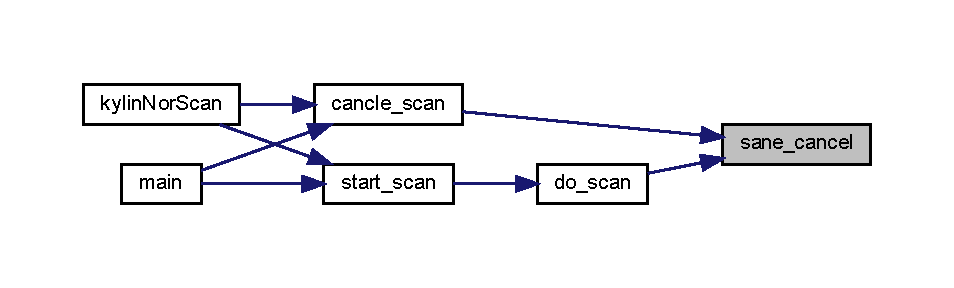
\includegraphics[width=350pt]{sane_8h_a8facc0281b730ce19e17971e5c042de1_icgraph}
\end{center}
\end{figure}
\mbox{\Hypertarget{sane_8h_a86bc6c8bf32a9e1ab2dc681dcf8489f1}\label{sane_8h_a86bc6c8bf32a9e1ab2dc681dcf8489f1}} 
\index{sane.h@{sane.h}!sane\_close@{sane\_close}}
\index{sane\_close@{sane\_close}!sane.h@{sane.h}}
\doxysubsubsection{\texorpdfstring{sane\_close()}{sane\_close()}}
{\footnotesize\ttfamily void sane\+\_\+close (\begin{DoxyParamCaption}\item[{\mbox{\hyperlink{sane_8h_adff38d40c72e14125709194edfd45e1b}{S\+A\+N\+E\+\_\+\+Handle}}}]{handle }\end{DoxyParamCaption})}

此函数终止在参数h中传递的设备句柄与其表示的设备之间的关联。 如果设备当前处于活动状态,则首先执行对sane\+\_\+cancel()的调用。此函数返回后,不能再使用句柄h。 这是这个函数的调用关系图\+:\nopagebreak
\begin{figure}[H]
\begin{center}
\leavevmode
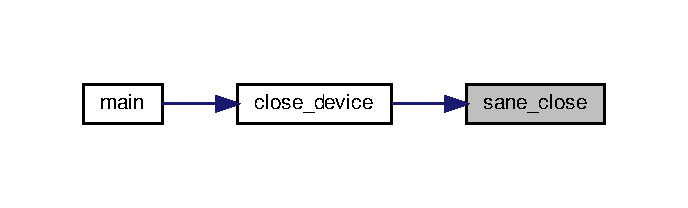
\includegraphics[width=330pt]{sane_8h_a86bc6c8bf32a9e1ab2dc681dcf8489f1_icgraph}
\end{center}
\end{figure}
\mbox{\Hypertarget{sane_8h_af97b5a648c359cdeb17844f24e74f21d}\label{sane_8h_af97b5a648c359cdeb17844f24e74f21d}} 
\index{sane.h@{sane.h}!sane\_control\_option@{sane\_control\_option}}
\index{sane\_control\_option@{sane\_control\_option}!sane.h@{sane.h}}
\doxysubsubsection{\texorpdfstring{sane\_control\_option()}{sane\_control\_option()}}
{\footnotesize\ttfamily \mbox{\hyperlink{sane_8h_ae5ce8ba47cee42542d1a981be4e4c552}{S\+A\+N\+E\+\_\+\+Status}} sane\+\_\+control\+\_\+option (\begin{DoxyParamCaption}\item[{\mbox{\hyperlink{sane_8h_adff38d40c72e14125709194edfd45e1b}{S\+A\+N\+E\+\_\+\+Handle}}}]{handle,  }\item[{\mbox{\hyperlink{sane_8h_a18b0de32eae6997909ae9ab0117af3d5}{S\+A\+N\+E\+\_\+\+Int}}}]{option,  }\item[{\mbox{\hyperlink{sane_8h_a676e37749b97063237ac22f5d8ae7cd7}{S\+A\+N\+E\+\_\+\+Action}}}]{action,  }\item[{void $\ast$}]{value,  }\item[{\mbox{\hyperlink{sane_8h_a18b0de32eae6997909ae9ab0117af3d5}{S\+A\+N\+E\+\_\+\+Int}} $\ast$}]{info }\end{DoxyParamCaption})}

此功能用于设置或查询由句柄h表示的设备的选件编号n的当前值。 选项a的控制方式由参数a指定 。该参数的可能值将在下面更详细地描述。 该选项的值通过参数v传递 。它是指向保存选项值的内存的指针。 v指向的内存区域必须足够大以容纳整个选项值(由相应选项描述符中的成员大小确定)。 该规则的唯一例外是,在设置字符串选项的值时,参数v指向的字符串可能会更短,因为在遇到 字符串中的第一个\+N\+U\+L终止符时,后端将停止读取选项值。 如果参数i不为\+N\+U\+L\+L,则将设置$\ast$ i的值以提供有关如何满足请求的详细信息。该参数的含义将在下面更详细地描述。

通过调用此函数影响选项的方式由参数a控制,参数a是\+S\+A\+N\+E\+\_\+\+Action类型的值 。可能的值及其含义在表7中描述。

符号 码 描述

S\+A\+N\+E\+\_\+\+A\+C\+T\+I\+O\+N\+\_\+\+G\+E\+T\+\_\+\+V\+A\+L\+UE 0 获取当前的期权价值。

S\+A\+N\+E\+\_\+\+A\+C\+T\+I\+O\+N\+\_\+\+S\+E\+T\+\_\+\+V\+A\+L\+UE 1 设置选项值。如果无法精确设置通过参数v传递的选项值,则后端可能会对其进行修改。

S\+A\+N\+E\+\_\+\+A\+C\+T\+I\+O\+N\+\_\+\+S\+E\+T\+\_\+\+A\+U\+TO 2 打开自动模式。后端或设备将自动选择适当的值。此模式将保持有效,直到被显式设置值请求覆盖为止。 在这种情况下,参数v的值将被完全忽略,并且可以为\+N\+U\+L\+L。

通过\+S\+A\+N\+E\+\_\+\+A\+C\+T\+I\+O\+N\+\_\+\+S\+E\+T\+\_\+\+V\+A\+L\+U\+E的操作值设置一个值后 ,在$\ast$ i中返回有关如何满足请求的其他信息(如果i为非\+N\+U\+L\+L)。返回的值是一个位集,可以包含表8中描述的值的任何组合。

符号 码 描述

S\+A\+N\+E\+\_\+\+I\+N\+F\+O\+\_\+\+I\+N\+E\+X\+A\+CT 1 当设置选项值导致选择的值与请求的值不完全匹配时,将返回此值。 例如,如果扫描仪只能以30dpi的增量调整分辨率,则将分辨率设置为307dpi可能会导致实际设置为300dpi。 发生这种情况时,$\ast$ i中返回的位集具有此成员集。另外,修改了选项值以反映后端使用的实际(四舍五入)值。 请注意,字符串也可以使用不精确的值。后端可以选择将字符串\`{}`舍入'\textquotesingle{}到最接近的匹配合法字符串以获取受约束的字符串值。

S\+A\+N\+E\+\_\+\+I\+N\+F\+O\+\_\+\+R\+E\+L\+O\+A\+D\+\_\+\+O\+P\+T\+I\+O\+NS 2 选项的设置可能会影响一个或多个 其他选项的价值或可用性。 发生这种情况时,\+S\+A\+N\+E后端会在$\ast$ i中设置此成员,以指示应用程序应重新加载所有选项。 仅当更改了至少一个选项时,才能设置此成员。

S\+A\+N\+E\+\_\+\+I\+N\+F\+O\+\_\+\+R\+E\+L\+O\+A\+D\+\_\+\+P\+A\+R\+A\+MS 4 选项的设置可能会影响参数值(请参见sane\+\_\+get\+\_\+parameters())。 如果设置选项影响参数值,则该成员将在$\ast$ i中设置。请注意,即使参数没有实际更改,也可以设置该成员。 但是,可以确保不设置此成员就不会更改参数。

此功能可能因以下状态代码之一而失败。

S\+A\+N\+E\+\_\+\+S\+T\+A\+T\+U\+S\+\_\+\+U\+N\+S\+U\+P\+P\+O\+R\+T\+E\+D:

指定的句柄和选项号不支持该操作。

S\+A\+N\+E\+\_\+\+S\+T\+A\+T\+U\+S\+\_\+\+I\+N\+V\+A\+L:

选项值无效。

S\+A\+N\+E\+\_\+\+S\+T\+A\+T\+U\+S\+\_\+\+I\+O\+\_\+\+E\+R\+R\+O\+R:

与设备通信时发生错误。

S\+A\+N\+E\+\_\+\+S\+T\+A\+T\+U\+S\+\_\+\+N\+O\+\_\+\+M\+E\+M:

可用的内存量不足。

S\+A\+N\+E\+\_\+\+S\+T\+A\+T\+U\+S\+\_\+\+A\+C\+C\+E\+S\+S\+\_\+\+D\+E\+N\+I\+E\+D:

由于身份验证不充分或无效,因此无法访问该选件。 \mbox{\Hypertarget{sane_8h_adee134f0b60b099d3ddb144ec7266c6a}\label{sane_8h_adee134f0b60b099d3ddb144ec7266c6a}} 
\index{sane.h@{sane.h}!sane\_exit@{sane\_exit}}
\index{sane\_exit@{sane\_exit}!sane.h@{sane.h}}
\doxysubsubsection{\texorpdfstring{sane\_exit()}{sane\_exit()}}
{\footnotesize\ttfamily void sane\+\_\+exit (\begin{DoxyParamCaption}\item[{void}]{ }\end{DoxyParamCaption})}



退出后端 


\begin{DoxyPre}\end{DoxyPre}



\begin{DoxyPre}必须调用此函数以终止使用后端。
该函数将首先关闭所有可能仍处于打开状态的设备句柄(建议通过调用sane\_close()显式关闭设备句柄,但要求后端在调用此函数时释放所有资源)。
此函数返回后,不能调用sane\_init()以外的任何函数(无论sane\_exit()返回的状态值如何。忽略调用此函数可能会导致某些资源无法正确释放。
\end{DoxyPre}



\begin{DoxyParams}{参数}
{\em a} & 变量a \\
\hline
{\em a} & 变量a \\
\hline
\end{DoxyParams}
\begin{DoxyReturn}{返回}
void 
\end{DoxyReturn}

\begin{DoxyRetVals}{返回值}
{\em 1} & result1 2\+: result2 \\
\hline
\end{DoxyRetVals}
这是这个函数的调用关系图\+:\nopagebreak
\begin{figure}[H]
\begin{center}
\leavevmode
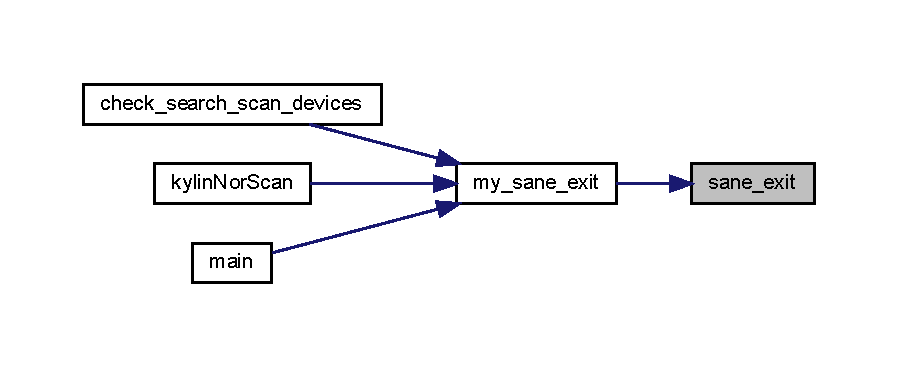
\includegraphics[width=326pt]{sane_8h_adee134f0b60b099d3ddb144ec7266c6a_icgraph}
\end{center}
\end{figure}
\mbox{\Hypertarget{sane_8h_a86a720cead710936ba84b6de59b16623}\label{sane_8h_a86a720cead710936ba84b6de59b16623}} 
\index{sane.h@{sane.h}!sane\_get\_devices@{sane\_get\_devices}}
\index{sane\_get\_devices@{sane\_get\_devices}!sane.h@{sane.h}}
\doxysubsubsection{\texorpdfstring{sane\_get\_devices()}{sane\_get\_devices()}}
{\footnotesize\ttfamily \mbox{\hyperlink{sane_8h_ae5ce8ba47cee42542d1a981be4e4c552}{S\+A\+N\+E\+\_\+\+Status}} sane\+\_\+get\+\_\+devices (\begin{DoxyParamCaption}\item[{const \mbox{\hyperlink{structSANE__Device}{S\+A\+N\+E\+\_\+\+Device}} $\ast$$\ast$$\ast$}]{device\+\_\+list,  }\item[{\mbox{\hyperlink{sane_8h_afb77ef4d4ce97f57e5a9e54393f979ee}{S\+A\+N\+E\+\_\+\+Bool}}}]{local\+\_\+only }\end{DoxyParamCaption})}

此功能可用于查询可用设备的列表。 如果函数成功执行,它将 在$\ast$ device\+\_\+list中存储指向\+N\+U\+L\+L终止数组的指针,该数组指向\+S\+A\+N\+E\+\_\+\+Device结构。 保证返回的列表保持不变并有效,直到(a)对该函数的另一次调用或(b)对sane\+\_\+exit()的调用。 可以重复调用此功能以检测何时有新设备可用。如果参数local\+\_\+only为true,则仅返回本地设备(直接连接到运行\+S\+A\+N\+E的计算机的设备)。 如果为假,则设备列表包括\+S\+A\+N\+E库可访问的所有远程设备。

如果没有足够的内存,此功能可能会因\+S\+A\+N\+E\+\_\+\+S\+T\+A\+T\+U\+S\+\_\+\+N\+O\+\_\+\+M\+E\+M而失败。

后端实施说明 S\+A\+N\+E不需要在执行sane\+\_\+open()调用之前调用此函数 。设备名称可以由用户明确指定,这将导致不必要且不希望先调用此功能。 这是这个函数的调用关系图\+:\nopagebreak
\begin{figure}[H]
\begin{center}
\leavevmode
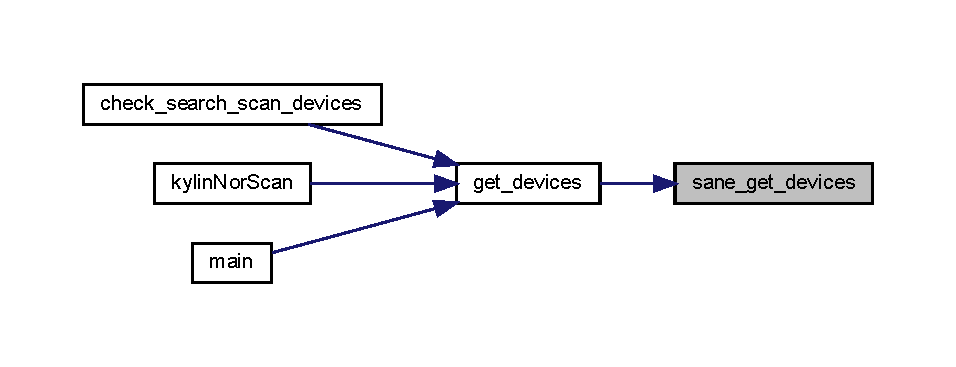
\includegraphics[width=350pt]{sane_8h_a86a720cead710936ba84b6de59b16623_icgraph}
\end{center}
\end{figure}
\mbox{\Hypertarget{sane_8h_a7728e01a38c5e18385e383a6ce4a108d}\label{sane_8h_a7728e01a38c5e18385e383a6ce4a108d}} 
\index{sane.h@{sane.h}!sane\_get\_option\_descriptor@{sane\_get\_option\_descriptor}}
\index{sane\_get\_option\_descriptor@{sane\_get\_option\_descriptor}!sane.h@{sane.h}}
\doxysubsubsection{\texorpdfstring{sane\_get\_option\_descriptor()}{sane\_get\_option\_descriptor()}}
{\footnotesize\ttfamily const \mbox{\hyperlink{structSANE__Option__Descriptor}{S\+A\+N\+E\+\_\+\+Option\+\_\+\+Descriptor}}$\ast$ sane\+\_\+get\+\_\+option\+\_\+descriptor (\begin{DoxyParamCaption}\item[{\mbox{\hyperlink{sane_8h_adff38d40c72e14125709194edfd45e1b}{S\+A\+N\+E\+\_\+\+Handle}}}]{handle,  }\item[{\mbox{\hyperlink{sane_8h_a18b0de32eae6997909ae9ab0117af3d5}{S\+A\+N\+E\+\_\+\+Int}}}]{option }\end{DoxyParamCaption})}

此函数用于访问选项描述符。该函数返回由句柄h表示的设备的选项号n的选项描述符。 选项号0保证是有效的选项。它的值是一个整数,它指定可用于设备句柄h的选项数量(计数包括选项0)。 如果n不是有效的选项索引,则该函数返回\+N\+U\+L\+L。保证返回的选项描述符在关闭设备之前一直保持有效(并在返回的地址处)。 \mbox{\Hypertarget{sane_8h_a28ba54307cb61e48fc1a361be7ad2c6e}\label{sane_8h_a28ba54307cb61e48fc1a361be7ad2c6e}} 
\index{sane.h@{sane.h}!sane\_get\_parameters@{sane\_get\_parameters}}
\index{sane\_get\_parameters@{sane\_get\_parameters}!sane.h@{sane.h}}
\doxysubsubsection{\texorpdfstring{sane\_get\_parameters()}{sane\_get\_parameters()}}
{\footnotesize\ttfamily \mbox{\hyperlink{sane_8h_ae5ce8ba47cee42542d1a981be4e4c552}{S\+A\+N\+E\+\_\+\+Status}} sane\+\_\+get\+\_\+parameters (\begin{DoxyParamCaption}\item[{\mbox{\hyperlink{sane_8h_adff38d40c72e14125709194edfd45e1b}{S\+A\+N\+E\+\_\+\+Handle}}}]{handle,  }\item[{\mbox{\hyperlink{structSANE__Parameters}{S\+A\+N\+E\+\_\+\+Parameters}} $\ast$}]{params }\end{DoxyParamCaption})}

此功能用于获取当前的扫描参数。 在开始扫描(调用sane\+\_\+start())与完成请求之间,保证返回的参数是准确的。 在该窗口之外,返回值是在调用sane\+\_\+start()时参数将尽力而为的估计 。 例如,在实际开始扫描之前调用此函数可以例如估算出扫描图像的大小。 传递给此函数的参数是应为其获取参数的设备的句柄h,以及指向参数结构的指针p。参数结构在下面更详细地描述。 扫描参数以\+S\+A\+N\+E\+\_\+\+Parameters类型的结构返回 。 这是这个函数的调用关系图\+:\nopagebreak
\begin{figure}[H]
\begin{center}
\leavevmode
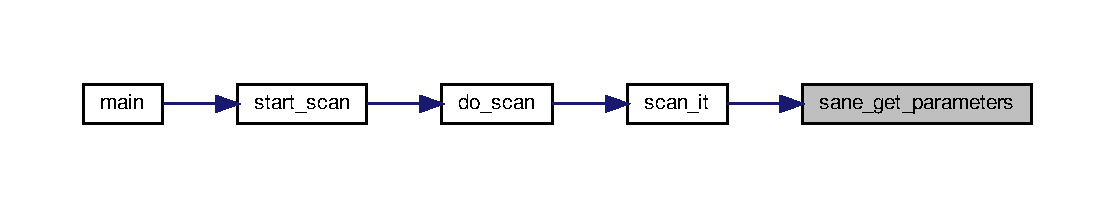
\includegraphics[width=350pt]{sane_8h_a28ba54307cb61e48fc1a361be7ad2c6e_icgraph}
\end{center}
\end{figure}
\mbox{\Hypertarget{sane_8h_a6699a6bb08baa461b98d62fcdd82d8d4}\label{sane_8h_a6699a6bb08baa461b98d62fcdd82d8d4}} 
\index{sane.h@{sane.h}!sane\_get\_select\_fd@{sane\_get\_select\_fd}}
\index{sane\_get\_select\_fd@{sane\_get\_select\_fd}!sane.h@{sane.h}}
\doxysubsubsection{\texorpdfstring{sane\_get\_select\_fd()}{sane\_get\_select\_fd()}}
{\footnotesize\ttfamily \mbox{\hyperlink{sane_8h_ae5ce8ba47cee42542d1a981be4e4c552}{S\+A\+N\+E\+\_\+\+Status}} sane\+\_\+get\+\_\+select\+\_\+fd (\begin{DoxyParamCaption}\item[{\mbox{\hyperlink{sane_8h_adff38d40c72e14125709194edfd45e1b}{S\+A\+N\+E\+\_\+\+Handle}}}]{handle,  }\item[{\mbox{\hyperlink{sane_8h_a18b0de32eae6997909ae9ab0117af3d5}{S\+A\+N\+E\+\_\+\+Int}} $\ast$}]{fd }\end{DoxyParamCaption})}

此函数用于获取句柄h的(特定于平台的)文件描述符 当且仅当图像数据可用时(即,对sane\+\_\+read()的调用将返回至少一个字节的数据),该文件描述符才可读。如果调用成功完成,则在$\ast$ fd中返回选择文件描述符。 仅在执行对sane\+\_\+start()的调用 并且已保证返回的文件描述符在当前图像获取期间保持有效 (即,直到再次调用sane\+\_\+cancel()或sane\+\_\+start()或直到sane\+\_\+read()返回状态 S\+A\+N\+E\+\_\+\+S\+T\+A\+T\+U\+S\+\_\+\+E\+O\+F)。 实际上,后端必须保证在下一个sane\+\_\+read()调用返回\+S\+A\+N\+E\+\_\+\+S\+T\+A\+T\+U\+S\+\_\+\+E\+O\+F时关闭返回的选择 文件描述符。 这是确保应用程序可以检测到何时发生这种情况而不必实际调用sane\+\_\+read()所必需的。

后端可以选择不支持此操作。在这种情况下,该函数将返回状态码 S\+A\+N\+E\+\_\+\+S\+T\+A\+T\+U\+S\+\_\+\+U\+N\+S\+U\+P\+P\+O\+R\+T\+E\+D。

请注意,返回的文件描述符支持的唯一操作是与主机操作系统相关的测试,以确定文件描述符是否可读 (例如,可以在\+U\+N\+I\+X下使用select() 或poll()来实现此测试)。如果对文件描述符执行任何其他操作,则后端的行为将变得不可预测。 一旦文件描述符发出\`{}`可读'\textquotesingle{}状态的信号,它将保持该状态,直到执行对sane\+\_\+read()的调用为止。 由于许多输入设备非常慢,因此强烈建议支持此操作,因为它允许应用程序在进行图像采集时执行其他工作。

此功能可能因以下状态代码之一而失败: \begin{DoxyVerb}SANE_STATUS_INVAL:

没有图像采集正在等待。

SANE_STATUS_UNSUPPORTED:

后端不支持此操作。
\end{DoxyVerb}
 \mbox{\Hypertarget{sane_8h_a1498918f9c7e543a4a757482bcffd7a9}\label{sane_8h_a1498918f9c7e543a4a757482bcffd7a9}} 
\index{sane.h@{sane.h}!sane\_init@{sane\_init}}
\index{sane\_init@{sane\_init}!sane.h@{sane.h}}
\doxysubsubsection{\texorpdfstring{sane\_init()}{sane\_init()}}
{\footnotesize\ttfamily \mbox{\hyperlink{sane_8h_ae5ce8ba47cee42542d1a981be4e4c552}{S\+A\+N\+E\+\_\+\+Status}} sane\+\_\+init (\begin{DoxyParamCaption}\item[{\mbox{\hyperlink{sane_8h_a18b0de32eae6997909ae9ab0117af3d5}{S\+A\+N\+E\+\_\+\+Int}} $\ast$}]{version\+\_\+code,  }\item[{\mbox{\hyperlink{sane_8h_a65071043cb6021bddedc7f249d9338ea}{S\+A\+N\+E\+\_\+\+Auth\+\_\+\+Callback}}}]{authorize }\end{DoxyParamCaption})}


\begin{DoxyPre}
  代码流\end{DoxyPre}



\begin{DoxyPre}  -\/\mbox{\hyperlink{sane_8h_a1498918f9c7e543a4a757482bcffd7a9}{sane\_init()}}
       -\/pick desired device, possibly by using \mbox{\hyperlink{sane_8h_a86a720cead710936ba84b6de59b16623}{sane\_get\_devices()}}
       -\/\mbox{\hyperlink{sane_8h_adfeda33e4d60e0d6a4e19634cc9c2bae}{sane\_open()}}
           //device setup
           -\/use: 
                   sane\_get\_option\_description()
                   \mbox{\hyperlink{sane_8h_af97b5a648c359cdeb17844f24e74f21d}{sane\_control\_option()}}
           repeatedly to configure device as desired\end{DoxyPre}



\begin{DoxyPre}           //image acquisition
           -\/\mbox{\hyperlink{sane_8h_a633f90b105f09ca798ecbf9a77711e7b}{sane\_start()}}
           -\/use: 
                   \mbox{\hyperlink{sane_8h_a28ba54307cb61e48fc1a361be7ad2c6e}{sane\_get\_parameters()}}
                   \mbox{\hyperlink{sane_8h_ae5426bddf1bfe3d30370c9fe2d209cc3}{sane\_read()}}
           repeatedly until read returns EOF
           -\/go back to \mbox{\hyperlink{sane_8h_a633f90b105f09ca798ecbf9a77711e7b}{sane\_start()}} if more frames desired
       -\/\mbox{\hyperlink{sane_8h_a86bc6c8bf32a9e1ab2dc681dcf8489f1}{sane\_close()}}
  -\/\mbox{\hyperlink{sane_8h_adee134f0b60b099d3ddb144ec7266c6a}{sane\_exit()}}\end{DoxyPre}



\begin{DoxyPre}  流程详解:
  可以在调用sane\_init()之后的任何时间调用 函数sane\_get\_devices()。它返回呼叫时已知的设备列表。
  由于某些设备可能已打开或关闭,或者远程主机可能在不同的呼叫之间启动或关闭,因此该列表可能会随时间变化。
  应当注意,此操作可能相对较慢,因为它需要联系所有已配置的设备(其中一些可能在远程主机上)。
  因此,前端可能希望为用户提供直接选择所需设备的功能,而无需调用此功能。\end{DoxyPre}



\begin{DoxyPre}  选择设备后,可通过调用sane\_open()将其打开 。可以在任何给定时间打开多个设备。SANE后端不得在任何给定时间对可以打开多少个设备施加人为约束。\end{DoxyPre}



\begin{DoxyPre}  可以使用功能sane\_get\_option\_descriptor()和 sane\_control\_option()通过相应的设备句柄设置打开的设备。
  设置设备时,可以自由地混合使用选项描述符以及设置和读取选项值。前端通常会在开始时读出所有可用选项,
  然后建立一个对话框(图形或命令行选项列表),以控制可用选项。应当注意,对于给定的句柄,选项的数量是固定的。
  但是,随着选项的设置,其他选项可能会变为活动或非活动状态。因此,在设置选项之后,可能需要重新读取一些或所有选项描述符。
  设置设备时,也可以拨打电话 sane\_get\_parameters()以获取图像获取开始后图像参数的估算值。\end{DoxyPre}



\begin{DoxyPre}  通过调用sane\_set\_io\_mode()可以将设备句柄置于阻塞或非阻塞模式。
  要求设备支持阻止模式(这是默认模式),但是对于诸如UNIX之类的操作系统,强烈建议支持非阻止I / O。\end{DoxyPre}



\begin{DoxyPre}  正确设置设备后,可以通过调用sane\_start()来启动图像获取。后端此时会计算出确切的图像参数。
  因此,将来对sane\_get\_parameters()的调用 将返回确切的值,而不是估计值。
  SANE API未指定是在这一点上还是在第一次调用sane\_read()时开始物理图像获取。
  如果需要无阻塞的I / O和/或选择样式的接口,则前端可能会在此时尝试调用 sane\_set\_io\_mode()和/或sane\_get\_select\_fd()。
  如果后端不支持请求的操作,则这些功能中的任何一个都可能失败。\end{DoxyPre}



\begin{DoxyPre}  通过重复调用sane\_read()来收集图像数据。最终,此函数将返回文件结束状态(SANE\_STATUS\_EOF)。
  这指示当前帧的结束。如果前端需要其他帧(例如,红色/绿色/蓝色图像或多个图像中的各个通道),则可以再次调用sane\_start()。
  一旦获取了所有所需的帧,就必须调用函数sane\_cancel()。也可以在任何其他时间调用此操作以取消挂起的操作。
  请注意,即使最后一次读取操作返回了SANE\_STATUS\_EOF,也必须调用sane\_cancel()。\end{DoxyPre}



\begin{DoxyPre}  使用设备完成操作后,应通过调用sane\_close()关闭句柄 。最后,在退出应用程序之前,必须调用函数sane\_exit()。
  重要的是不要忘记调用此函数,否则可能会导致某些资源(例如临时文件或锁)无人认领。\end{DoxyPre}



\begin{DoxyPre}  其他选项
  尽管大多数后端选项都是完全自描述的,但在某些情况下,用户界面可能希望对某些选项进行特殊处理。
  例如,扫描区域通常由四个选项定义,这些选项指定区域的左上角和右下角。使用图形用户界面,迫使用户键入这四个数字将很繁琐。
  相反,大多数此类界面都希望向用户呈现扫描仪表面的预览(低分辨率扫描),并让用户通过将矩形拖动到所需位置来选择扫描区域。
  因此,SANE API指定了少数具有明确定义含义的选项名称。\end{DoxyPre}



\begin{DoxyPre}  选件编号计数
  选项号0的名称为空字符串。此选项的值的类型为SANE\_TYPE\_INT,它指定给定设备可用的选项总数(计数包括选项号0)。
  这意味着有两种计算可用选项数量的方法:前端可以循环从一个选项开始的所有选项编号,
  直到 sane\_get\_option\_descriptor()返回NULL,或者前端可以直接读出选项编号0的值。\end{DoxyPre}



\begin{DoxyPre}  扫描分辨率选项
  选项分辨率用于选择应获取图像的分辨率。此选项的类型为 SANE\_TYPE\_INT或SANE\_TYPE\_FIXED。单位是 SANE\_UNIT\_DPI(点/英寸)。
  此选项不是强制性的,但是如果后端确实支持它,则它必须以与上述定义一致的方式来实现。\end{DoxyPre}



\begin{DoxyPre}  预览模式选项
  前端使用布尔选项预览来通知后端何时应针对速度而非质量(``预览模式'')优化图像采集。
  设置为SANE\_TRUE时,预览模式有效;设置为SANE\_FALSE时,图像采集应以普通质量模式进行。
  此选项的设置不得影响任何其他选项。也就是说,就其他选项而言,预览模式完全没有副作用。
  后端可以假定前端将适当地设置预览模式的扫描分辨率(通过option resolution)。
  后端可以随意覆盖 分辨率 可以选择自己的预览模式,但建议尽可能将其保留在前端。
  此选项不是强制性的,但是如果后端确实支持它,则它必须以与上述定义一致的方式来实现。\end{DoxyPre}



\begin{DoxyPre}  扫描区域选项
  四个最重要的众所周知的选项是定义扫描区域的选项。扫描区域由指定左上角和右下角的两个点(x / y坐标对)定义。
  这在图5中示出。请注意,坐标系的原点位于传感器所看到的扫描表面的左上角(通常是用户看到的扫描表面的镜像)。
  因此,左上角是横坐标和纵坐标值同时最小的角,右下角是横坐标和纵坐标值近似最大的角。
  如果此坐标系对于给定的设备而言不是自然的,则后端的工作就是执行必要的转换。\end{DoxyPre}



\begin{DoxyPre}× 扫描区域选项
                                               → x
        0 -\/-\/-\/-\/-\/-\/-\/-\/-\/-\/-\/-\/-\/-\/-\/-\/-\/-\/-\/-\/-\/-\/-\/-\/-\/-\/-\/-\/-\/-\/-\/-\/-\/-\/-\/-\/-\/-\/
        |             scan surface             |
        |                                      |
        |                                      |
        |      top-\/left                        |
        |          -\/-\/-\/-\/-\/-\/-\/-\/-\/-\/-\/-\/-\/-\/-\/-\/-\/           |
        |          |  scan area    |           |
        |          -\/-\/-\/-\/-\/-\/-\/-\/-\/-\/-\/-\/-\/-\/-\/-\/-\/           |
        |                       bottom-\/right   |
        |                                      |
        |                                      |
   ↓ y  |-\/-\/-\/-\/-\/-\/-\/-\/-\/-\/-\/-\/-\/-\/-\/-\/-\/-\/-\/-\/-\/-\/-\/-\/-\/-\/-\/-\/-\/-\/-\/-\/-\/-\/-\/-\/-\/-\/-\/\end{DoxyPre}



\begin{DoxyPre}  下表列出了定义扫描区域的四个选项的名称:
  名称    描述
  tl-\/x  左上角x坐标值
  tl-\/y  左上y坐标值
  br-\/x  右下x坐标值
  br-\/y  右下y坐标值\end{DoxyPre}



\begin{DoxyPre}  关于这些选项,前端和后端应遵循几个规则:\end{DoxyPre}



\begin{DoxyPre}      后端必须将像素(SANE\_UNIT\_PIXEL)或毫米(SANE\_UNIT\_MM)的单位附加到这些选项。所有四个选项的单位必须相同。
      每当有意义时,后端应将范围或单词列表约束附加到这些选项。
      前端可以通过首先检查选项是否具有关联的范围约束来确定扫描表面的大小。
      如果存在范围或单词列表约束,则前端可以采用x和y选项范围约束之一的最小值和最大值来确定扫描表面大小。
      前端必须正确运行,而缺少任何或所有这些选项。\end{DoxyPre}



\begin{DoxyPre}  网络协议
  SANE接口的设计,方便图像采集设备的网络接入。特别是,
  大多数SANE实施都有望支持网络后端(网络客户端)和相应的网络守护程序(网络服务器),
  该网络后台程序允许通过网络连接访问图像采集设备。网络访问在以下几种情况下很有用:
       1)为了提供给那些无法进入正规的用户资源受控访问。例如,用户可能想访问没有帐户的主机上的设备。
          使用网络协议,可以允许某些用户访问扫描仪而无需给予他们对系统的完全访问权限。\end{DoxyPre}



\begin{DoxyPre}       2) 即使在本地情况下,通过网络守护程序控制访问也会很有用:例如,某些后端可能需要root特权才能访问设备。
           系统管理员可以将SANE网络守护程序安装为setuid-\/root,而不是将每个前端都安装为setuid-\/root。
           这使普通用户可以通过SANE守护程序访问特权设备(该守护程序可能比简单的setuid方法支持更细粒度的访问控制机制)。
           这具有额外的好处,即系统管理员只需要信任SANE守护程序,而不是可能需要访问特权设备的每个前端。
           网络访问提供了可用的图像采集设备的普及之感。例如,在局域网环境中,这允许用户登录到任何计算机上,
           并可以方便地访问网络上任何计算机可用的任何资源(受权限限制)。\end{DoxyPre}



\begin{DoxyPre}       3)对于使用时不需要物理访问的设备(例如摄像机),网络访问允许用户控制和使用这些设备而无需物理接近。
           实际上,如果将此类设备连接到Internet,则可以从世界上任何地方进行访问。\end{DoxyPre}



\begin{DoxyPre}  在设计本章中描述的网络协议时,要牢记以下目标:\end{DoxyPre}



\begin{DoxyPre}      1. 图像传输应该高效(编码开销较低)。
      2. 在客户端访问选项描述符必须高效(因为这是非常常见的操作)。
      3. 其他操作(如设置或查询选项的值)对性能的要求不高,因为它们通常需要明确的用户操作。
      4. 网络协议应该简单易行,可以在任何主机体系结构和任何编程语言上实现。\end{DoxyPre}



\begin{DoxyPre}  SANE协议可以在任何提供可靠数据传输的传输协议上运行。尽管SANE没有指定特定的传输协议,但是可以预期TCP / IP将成为最常用的协议之一。\end{DoxyPre}



\begin{DoxyPre}  \end{DoxyPre}
 初始化后端 必须先调用此函数,然后才能调用任何其他\+S\+A\+N\+E函数。 如果此功能未先叫或\+S\+A\+N\+E后端的行为都是不确定如果返回的状态代码sane\+\_\+init不同于 S\+A\+N\+E\+\_\+\+S\+T\+A\+T\+U\+S\+\_\+\+G\+O\+O\+D。 后端的版本代码以version\+\_\+code指向的值返回。如果该指针为 N\+U\+L\+L,则不返回任何版本代码。 参数授权是指向后端要求对特定资源进行身份验证时调用的函数的指针,或者如果前端不支持身份验证则为\+N\+U\+L\+L。

后端可以响应以下任何调用来调用授权功能:

sane\+\_\+open,sane\+\_\+control\+\_\+option,sane\+\_\+start

如果后端在没有授权功能的情况下初始化,那么后端本身无法处理的授权请求将自动失败,并且可能会阻止用户访问受保护的资源。 鼓励后端实施不需要用户协助的身份验证方法。例如,在通过登录过程验证用户身份的多用户系统上,后端可以根据资源和用户名自动查找适当的密码。 这是这个函数的调用关系图\+:\nopagebreak
\begin{figure}[H]
\begin{center}
\leavevmode
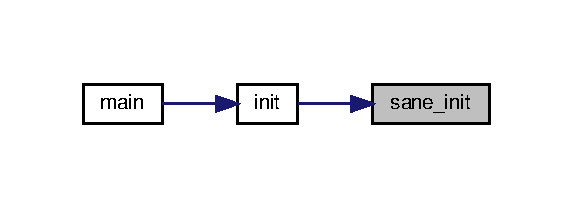
\includegraphics[width=275pt]{sane_8h_a1498918f9c7e543a4a757482bcffd7a9_icgraph}
\end{center}
\end{figure}
\mbox{\Hypertarget{sane_8h_adfeda33e4d60e0d6a4e19634cc9c2bae}\label{sane_8h_adfeda33e4d60e0d6a4e19634cc9c2bae}} 
\index{sane.h@{sane.h}!sane\_open@{sane\_open}}
\index{sane\_open@{sane\_open}!sane.h@{sane.h}}
\doxysubsubsection{\texorpdfstring{sane\_open()}{sane\_open()}}
{\footnotesize\ttfamily \mbox{\hyperlink{sane_8h_ae5ce8ba47cee42542d1a981be4e4c552}{S\+A\+N\+E\+\_\+\+Status}} sane\+\_\+open (\begin{DoxyParamCaption}\item[{\mbox{\hyperlink{sane_8h_a9a47323dab2a36db080f1bcc11585af4}{S\+A\+N\+E\+\_\+\+String\+\_\+\+Const}}}]{devicename,  }\item[{\mbox{\hyperlink{sane_8h_adff38d40c72e14125709194edfd45e1b}{S\+A\+N\+E\+\_\+\+Handle}} $\ast$}]{handle }\end{DoxyParamCaption})}

此功能用于建立到特定设备的连接。 要打开的设备的名称在参数name中传递 。如果调用成功完成,则在$\ast$ h中返回设备的句柄。 在特殊情况下,将零长度字符串指定为设备会请求打开第一个可用设备(如果有的话)。 此功能可能因以下状态代码之一而失败。

S\+A\+N\+E\+\_\+\+S\+T\+A\+T\+U\+S\+\_\+\+D\+E\+V\+I\+C\+E\+\_\+\+B\+U\+S\+Y: 设备当前正忙(其他人正在使用)。

S\+A\+N\+E\+\_\+\+S\+T\+A\+T\+U\+S\+\_\+\+I\+N\+V\+A\+L: 设备名称无效。

S\+A\+N\+E\+\_\+\+S\+T\+A\+T\+U\+S\+\_\+\+I\+O\+\_\+\+E\+R\+R\+O\+R: 与设备通信时发生错误。

S\+A\+N\+E\+\_\+\+S\+T\+A\+T\+U\+S\+\_\+\+N\+O\+\_\+\+M\+E\+M: 可用的内存量不足。

S\+A\+N\+E\+\_\+\+S\+T\+A\+T\+U\+S\+\_\+\+A\+C\+C\+E\+S\+S\+\_\+\+D\+E\+N\+I\+E\+D: 由于身份验证不充分或无效,因此无法访问设备。 这是这个函数的调用关系图\+:\nopagebreak
\begin{figure}[H]
\begin{center}
\leavevmode
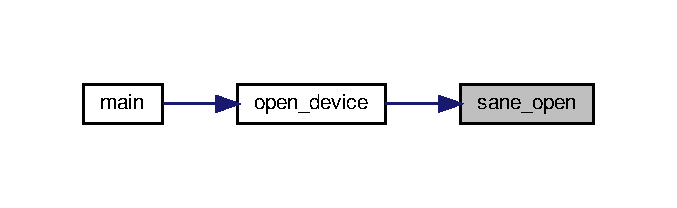
\includegraphics[width=325pt]{sane_8h_adfeda33e4d60e0d6a4e19634cc9c2bae_icgraph}
\end{center}
\end{figure}
\mbox{\Hypertarget{sane_8h_ae5426bddf1bfe3d30370c9fe2d209cc3}\label{sane_8h_ae5426bddf1bfe3d30370c9fe2d209cc3}} 
\index{sane.h@{sane.h}!sane\_read@{sane\_read}}
\index{sane\_read@{sane\_read}!sane.h@{sane.h}}
\doxysubsubsection{\texorpdfstring{sane\_read()}{sane\_read()}}
{\footnotesize\ttfamily \mbox{\hyperlink{sane_8h_ae5ce8ba47cee42542d1a981be4e4c552}{S\+A\+N\+E\+\_\+\+Status}} sane\+\_\+read (\begin{DoxyParamCaption}\item[{\mbox{\hyperlink{sane_8h_adff38d40c72e14125709194edfd45e1b}{S\+A\+N\+E\+\_\+\+Handle}}}]{handle,  }\item[{\mbox{\hyperlink{sane_8h_ae81a9c562538e486d29a0e86537763cf}{S\+A\+N\+E\+\_\+\+Byte}} $\ast$}]{data,  }\item[{\mbox{\hyperlink{sane_8h_a18b0de32eae6997909ae9ab0117af3d5}{S\+A\+N\+E\+\_\+\+Int}}}]{max\+\_\+length,  }\item[{\mbox{\hyperlink{sane_8h_a18b0de32eae6997909ae9ab0117af3d5}{S\+A\+N\+E\+\_\+\+Int}} $\ast$}]{length }\end{DoxyParamCaption})}

此功能用于从手柄h代表的设备中读取图像数据。 参数buf是一个指向至少maxlen个字节长的存储区的指针。返回的字节数存储在$\ast$ len中。当返回\+S\+A\+N\+E\+\_\+\+S\+T\+A\+T\+U\+S\+\_\+\+G\+O\+O\+D以外的状态时,后端必须将此值设置为零。当调用成功,返回的字节的数目可以在从0到的范围内的任何地方的maxlen字节。 如果在没有可用数据时调用此函数,则可能发生两种情况之一,具体取决于对句柄h生效的I / O模式。 \begin{DoxyVerb}如果设备处于阻止I / O模式(默认模式),则调用将阻止直到至少一个数据字节可用(或直到发生某些错误)为止。


如果设备处于非阻塞I / O模式,则调用立即返回,状态为SANE_STATUS_GOOD,并且 * len设置为零。
\end{DoxyVerb}


可以通过调用sane\+\_\+set\+\_\+io\+\_\+mode()来设置 句柄h的I / O模式。

此功能可能因以下状态代码之一而失败。 \begin{DoxyVerb}SANE_STATUS_CANCELLED:
通过调用sane_cancel取消了该操作。

SANE_STATUS_EOF:
当前帧没有更多数据。

SANE_STATUS_JAMMED:
文档进纸器被卡住。

SANE_STATUS_NO_DOCS:
文件进纸器中没有文件。

SANE_STATUS_COVER_OPEN:
扫描仪盖板打开。

SANE_STATUS_IO_ERROR:
与设备通信时发生错误。

SANE_STATUS_NO_MEM:
可用的内存量不足。

SANE_STATUS_ACCESS_DENIED:
由于身份验证不充分或无效,因此无法访问设备。
\end{DoxyVerb}
 这是这个函数的调用关系图\+:\nopagebreak
\begin{figure}[H]
\begin{center}
\leavevmode
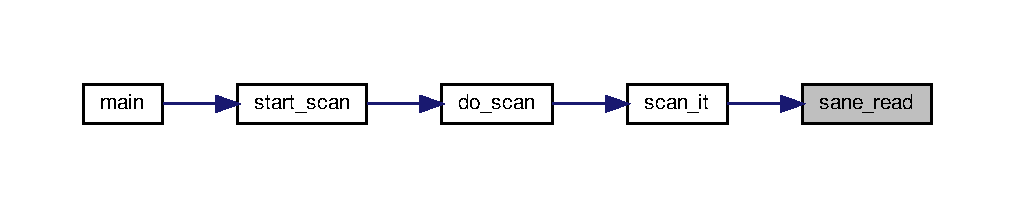
\includegraphics[width=350pt]{sane_8h_ae5426bddf1bfe3d30370c9fe2d209cc3_icgraph}
\end{center}
\end{figure}
\mbox{\Hypertarget{sane_8h_a1ee82e5f0a83ca9c96c17dbbba7cf543}\label{sane_8h_a1ee82e5f0a83ca9c96c17dbbba7cf543}} 
\index{sane.h@{sane.h}!sane\_set\_io\_mode@{sane\_set\_io\_mode}}
\index{sane\_set\_io\_mode@{sane\_set\_io\_mode}!sane.h@{sane.h}}
\doxysubsubsection{\texorpdfstring{sane\_set\_io\_mode()}{sane\_set\_io\_mode()}}
{\footnotesize\ttfamily \mbox{\hyperlink{sane_8h_ae5ce8ba47cee42542d1a981be4e4c552}{S\+A\+N\+E\+\_\+\+Status}} sane\+\_\+set\+\_\+io\+\_\+mode (\begin{DoxyParamCaption}\item[{\mbox{\hyperlink{sane_8h_adff38d40c72e14125709194edfd45e1b}{S\+A\+N\+E\+\_\+\+Handle}}}]{handle,  }\item[{\mbox{\hyperlink{sane_8h_afb77ef4d4ce97f57e5a9e54393f979ee}{S\+A\+N\+E\+\_\+\+Bool}}}]{non\+\_\+blocking }\end{DoxyParamCaption})}

此功能用于设置手柄h的I / O模式。 I / O模式可以是阻塞或非阻塞。如果参数m为 S\+A\+N\+E\+\_\+\+T\+R\+U\+E,则将模式设置为非阻塞模式,否则将其设置为阻塞模式。仅在对sane\+\_\+start()的调用完成后才能调用此函数 。 默认情况下,新打开的句柄以阻止模式运行。后端可以选择不支持非阻塞I / O模式。在这种情况下,将返回状态值\+S\+A\+N\+E\+\_\+\+S\+T\+A\+T\+U\+S\+\_\+\+U\+N\+S\+U\+P\+P\+O\+R\+T\+E\+D。 所有后端都必须支持阻塞I / O,因此可以确保将参数m设置为\+S\+A\+N\+E\+\_\+\+F\+A\+L\+S\+E调用此函数。

此功能可能因以下状态代码之一而失败: \begin{DoxyVerb}SANE_STATUS_INVAL:

没有图像采集正在等待。

SANE_STATUS_UNSUPPORTED:

后端不支持请求的I / O模式。
\end{DoxyVerb}
 \mbox{\Hypertarget{sane_8h_a633f90b105f09ca798ecbf9a77711e7b}\label{sane_8h_a633f90b105f09ca798ecbf9a77711e7b}} 
\index{sane.h@{sane.h}!sane\_start@{sane\_start}}
\index{sane\_start@{sane\_start}!sane.h@{sane.h}}
\doxysubsubsection{\texorpdfstring{sane\_start()}{sane\_start()}}
{\footnotesize\ttfamily \mbox{\hyperlink{sane_8h_ae5ce8ba47cee42542d1a981be4e4c552}{S\+A\+N\+E\+\_\+\+Status}} sane\+\_\+start (\begin{DoxyParamCaption}\item[{\mbox{\hyperlink{sane_8h_adff38d40c72e14125709194edfd45e1b}{S\+A\+N\+E\+\_\+\+Handle}}}]{handle }\end{DoxyParamCaption})}

此功能启动从手柄h表示的设备获取图像。 此功能可能因以下状态代码之一而失败。 \begin{DoxyVerb}SANE_STATUS_CANCELLED:
通过调用sane_cancel取消了该操作。

SANE_STATUS_DEVICE_BUSY:
设备忙。该操作应稍后重试。

SANE_STATUS_JAMMED:
文档进纸器被卡住。

SANE_STATUS_NO_DOCS:
文件进纸器中没有文件。

SANE_STATUS_COVER_OPEN:
扫描仪盖板打开。

SANE_STATUS_IO_ERROR:
与设备通信时发生错误。

SANE_STATUS_NO_MEM:
可用的内存量不足。

SANE_STATUS_INVAL:
无法使用当前选项集开始扫描。前端应该重新加载选项描述符,就像 SANE_INFO_RELOAD_OPTIONS已从对sane_control_option()的调用返回 ,因为设备的功能可能已更改。
\end{DoxyVerb}
 这是这个函数的调用关系图\+:\nopagebreak
\begin{figure}[H]
\begin{center}
\leavevmode
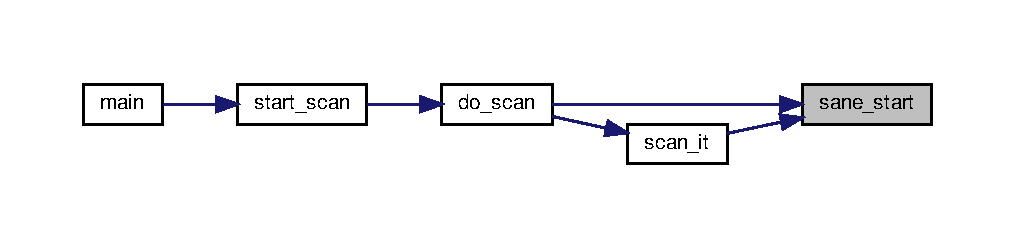
\includegraphics[width=350pt]{sane_8h_a633f90b105f09ca798ecbf9a77711e7b_icgraph}
\end{center}
\end{figure}
\mbox{\Hypertarget{sane_8h_a005fc36c746f3b57fcf8108435f0684d}\label{sane_8h_a005fc36c746f3b57fcf8108435f0684d}} 
\index{sane.h@{sane.h}!sane\_strstatus@{sane\_strstatus}}
\index{sane\_strstatus@{sane\_strstatus}!sane.h@{sane.h}}
\doxysubsubsection{\texorpdfstring{sane\_strstatus()}{sane\_strstatus()}}
{\footnotesize\ttfamily \mbox{\hyperlink{sane_8h_a9a47323dab2a36db080f1bcc11585af4}{S\+A\+N\+E\+\_\+\+String\+\_\+\+Const}} sane\+\_\+strstatus (\begin{DoxyParamCaption}\item[{\mbox{\hyperlink{sane_8h_ae5ce8ba47cee42542d1a981be4e4c552}{S\+A\+N\+E\+\_\+\+Status}}}]{status }\end{DoxyParamCaption})}

此功能可用于将\+S\+A\+N\+E状态代码转换为可打印的字符串。 返回的字符串是形成完整句子的单行文本,但没有结尾句号(句号)。该函数保证永远不会返回\+N\+U\+L\+L。返回的指针至少在下一次调用此函数之前是有效的。 这是这个函数的调用关系图\+:\nopagebreak
\begin{figure}[H]
\begin{center}
\leavevmode
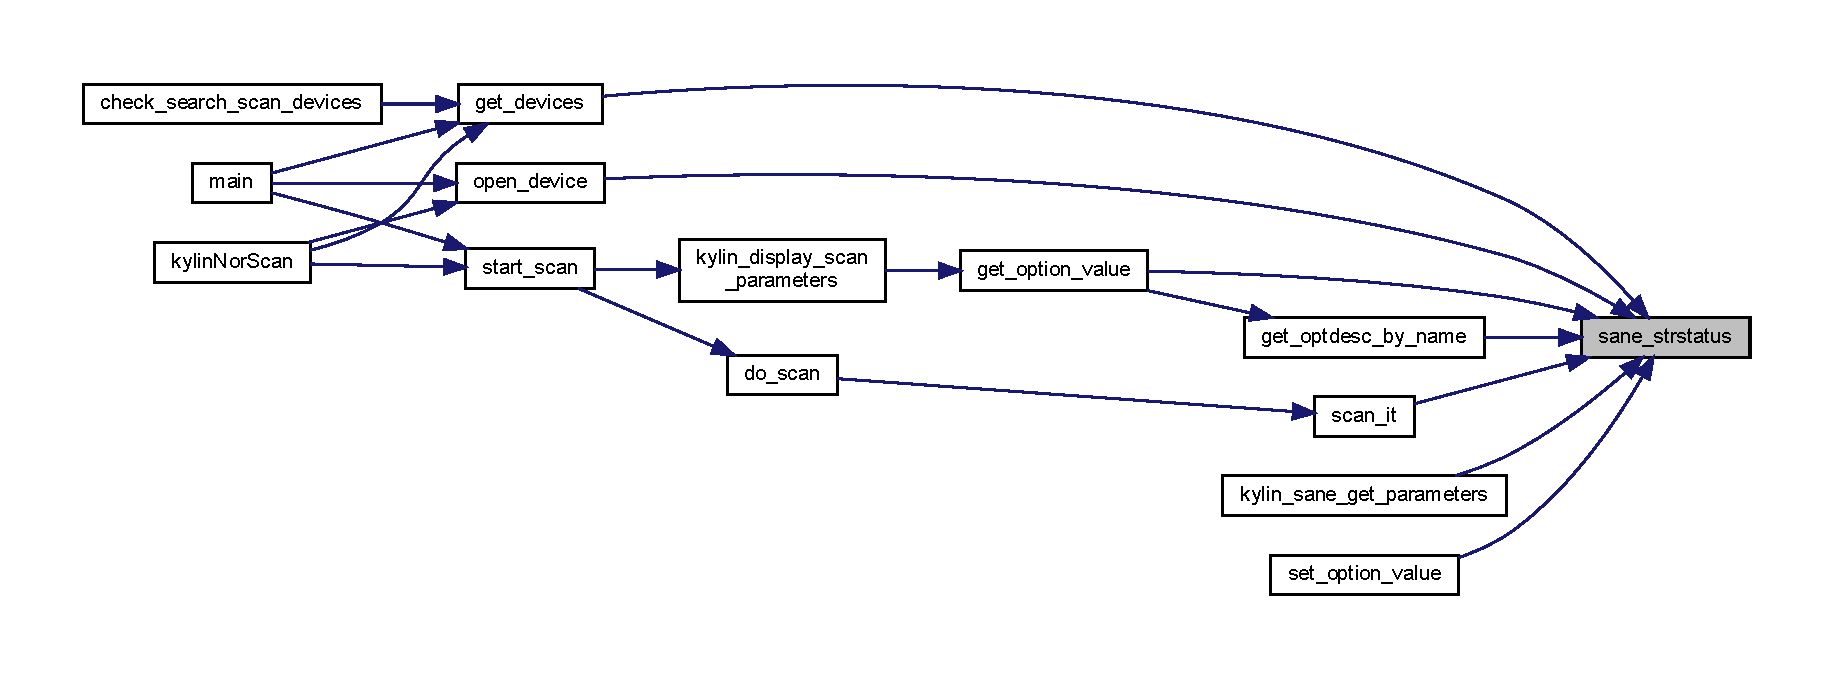
\includegraphics[width=342pt]{sane_8h_a005fc36c746f3b57fcf8108435f0684d_icgraph}
\end{center}
\end{figure}

\hypertarget{saneopts_8h}{}\doxysection{include/sane/saneopts.h 文件参考}
\label{saneopts_8h}\index{include/sane/saneopts.h@{include/sane/saneopts.h}}
此图展示该文件直接或间接的被哪些文件引用了\+:\nopagebreak
\begin{figure}[H]
\begin{center}
\leavevmode
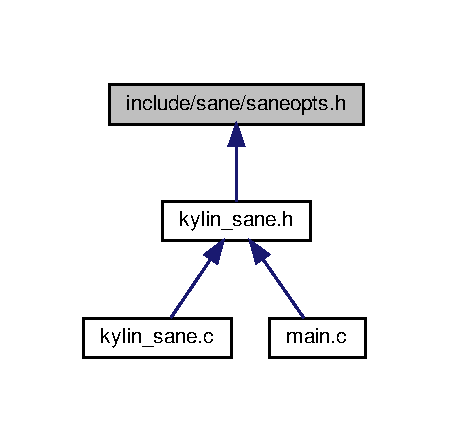
\includegraphics[width=216pt]{saneopts_8h__dep__incl}
\end{center}
\end{figure}
\doxysubsection*{宏定义}
\begin{DoxyCompactItemize}
\item 
\#define \mbox{\hyperlink{saneopts_8h_a3c672285cf8d02e3bbebb355c48c3ff9}{S\+A\+N\+E\+\_\+\+I18N}}(text)~text
\item 
\#define \mbox{\hyperlink{saneopts_8h_a2e76928a3e471db72cf87ff3d10691cc}{S\+A\+N\+E\+\_\+\+N\+A\+M\+E\+\_\+\+N\+U\+M\+\_\+\+O\+P\+T\+I\+O\+NS}}~\char`\"{}\char`\"{}	/$\ast$ never settable $\ast$/
\item 
\#define \mbox{\hyperlink{saneopts_8h_a170bf50e0ff8864a3c625c7fa719e9fb}{S\+A\+N\+E\+\_\+\+N\+A\+M\+E\+\_\+\+S\+T\+A\+N\+D\+A\+RD}}~\char`\"{}standard\char`\"{}
\item 
\#define \mbox{\hyperlink{saneopts_8h_a58cad59d9db5f4a66b4c2be55b8321c6}{S\+A\+N\+E\+\_\+\+N\+A\+M\+E\+\_\+\+G\+E\+O\+M\+E\+T\+RY}}~\char`\"{}geometry\char`\"{}
\item 
\#define \mbox{\hyperlink{saneopts_8h_a03673b3fbb5ae93e3400e88a996b5eb0}{S\+A\+N\+E\+\_\+\+N\+A\+M\+E\+\_\+\+E\+N\+H\+A\+N\+C\+E\+M\+E\+NT}}~\char`\"{}enhancement\char`\"{}
\item 
\#define \mbox{\hyperlink{saneopts_8h_a6d8b1b1b31e22bf5fc14f19fe29042e4}{S\+A\+N\+E\+\_\+\+N\+A\+M\+E\+\_\+\+A\+D\+V\+A\+N\+C\+ED}}~\char`\"{}advanced\char`\"{}
\item 
\#define \mbox{\hyperlink{saneopts_8h_aee7df0170ca5722585fa3a6f3d65daca}{S\+A\+N\+E\+\_\+\+N\+A\+M\+E\+\_\+\+S\+E\+N\+S\+O\+RS}}~\char`\"{}sensors\char`\"{}
\item 
\#define \mbox{\hyperlink{saneopts_8h_a089adf9ae5f36a7d01ee5fab704a2b8b}{S\+A\+N\+E\+\_\+\+N\+A\+M\+E\+\_\+\+P\+R\+E\+V\+I\+EW}}~\char`\"{}preview\char`\"{}
\item 
\#define \mbox{\hyperlink{saneopts_8h_a1f78cc2a74fcd1a55c272efd1811ec67}{S\+A\+N\+E\+\_\+\+N\+A\+M\+E\+\_\+\+G\+R\+A\+Y\+\_\+\+P\+R\+E\+V\+I\+EW}}~\char`\"{}preview-\/in-\/gray\char`\"{}
\item 
\#define \mbox{\hyperlink{saneopts_8h_a6b7f0f38abbc06183e1b3b6566e1ceb8}{S\+A\+N\+E\+\_\+\+N\+A\+M\+E\+\_\+\+B\+I\+T\+\_\+\+D\+E\+P\+TH}}~\char`\"{}depth\char`\"{}
\item 
\#define \mbox{\hyperlink{saneopts_8h_a06f72a185a3789fa0acd73a2fca302c1}{S\+A\+N\+E\+\_\+\+N\+A\+M\+E\+\_\+\+S\+C\+A\+N\+\_\+\+M\+O\+DE}}~\char`\"{}mode\char`\"{}
\item 
\#define \mbox{\hyperlink{saneopts_8h_a3a52567d2e4996caf0072d61fbdb2816}{S\+A\+N\+E\+\_\+\+N\+A\+M\+E\+\_\+\+S\+C\+A\+N\+\_\+\+S\+P\+E\+ED}}~\char`\"{}speed\char`\"{}
\item 
\#define \mbox{\hyperlink{saneopts_8h_a3dbe6c4d1c53b66787b6b57aa4439aed}{S\+A\+N\+E\+\_\+\+N\+A\+M\+E\+\_\+\+S\+C\+A\+N\+\_\+\+S\+O\+U\+R\+CE}}~\char`\"{}source\char`\"{}
\item 
\#define \mbox{\hyperlink{saneopts_8h_a191cd530d63d8e3b7066c95c87e6a45f}{S\+A\+N\+E\+\_\+\+N\+A\+M\+E\+\_\+\+B\+A\+C\+K\+T\+R\+A\+CK}}~\char`\"{}backtrack\char`\"{}
\item 
\#define \mbox{\hyperlink{saneopts_8h_a0db8d0a2ab36b8278de6ed461b7083ef}{S\+A\+N\+E\+\_\+\+N\+A\+M\+E\+\_\+\+S\+C\+A\+N\+\_\+\+T\+L\+\_\+X}}~\char`\"{}tl-\/x\char`\"{}
\item 
\#define \mbox{\hyperlink{saneopts_8h_aab8aa549c530dcf400b44257b1314bb0}{S\+A\+N\+E\+\_\+\+N\+A\+M\+E\+\_\+\+S\+C\+A\+N\+\_\+\+T\+L\+\_\+Y}}~\char`\"{}tl-\/y\char`\"{}
\item 
\#define \mbox{\hyperlink{saneopts_8h_a4f82ccb8b00c1da6f2d136498f94bb3e}{S\+A\+N\+E\+\_\+\+N\+A\+M\+E\+\_\+\+S\+C\+A\+N\+\_\+\+B\+R\+\_\+X}}~\char`\"{}br-\/x\char`\"{}
\item 
\#define \mbox{\hyperlink{saneopts_8h_ad83c04381585f3a0106356ecbc6e9b73}{S\+A\+N\+E\+\_\+\+N\+A\+M\+E\+\_\+\+S\+C\+A\+N\+\_\+\+B\+R\+\_\+Y}}~\char`\"{}br-\/y\char`\"{}
\item 
\#define \mbox{\hyperlink{saneopts_8h_ab8981b8aad7ae181f25e2774a6bf2182}{S\+A\+N\+E\+\_\+\+N\+A\+M\+E\+\_\+\+S\+C\+A\+N\+\_\+\+R\+E\+S\+O\+L\+U\+T\+I\+ON}}~\char`\"{}resolution\char`\"{}
\item 
\#define \mbox{\hyperlink{saneopts_8h_aaef35435fc2347918d4c20e9e458414c}{S\+A\+N\+E\+\_\+\+N\+A\+M\+E\+\_\+\+S\+C\+A\+N\+\_\+\+X\+\_\+\+R\+E\+S\+O\+L\+U\+T\+I\+ON}}~\char`\"{}x-\/resolution\char`\"{}
\item 
\#define \mbox{\hyperlink{saneopts_8h_a32eb4f9e26c1a5e644466972234a0f50}{S\+A\+N\+E\+\_\+\+N\+A\+M\+E\+\_\+\+S\+C\+A\+N\+\_\+\+Y\+\_\+\+R\+E\+S\+O\+L\+U\+T\+I\+ON}}~\char`\"{}y-\/resolution\char`\"{}
\item 
\#define \mbox{\hyperlink{saneopts_8h_a930b4aa4c780b9391bc1cc930fc6f381}{S\+A\+N\+E\+\_\+\+N\+A\+M\+E\+\_\+\+P\+A\+G\+E\+\_\+\+W\+I\+D\+TH}}~\char`\"{}page-\/width\char`\"{}
\item 
\#define \mbox{\hyperlink{saneopts_8h_aa83749b2cb7307380a0fcb85259fd06e}{S\+A\+N\+E\+\_\+\+N\+A\+M\+E\+\_\+\+P\+A\+G\+E\+\_\+\+H\+E\+I\+G\+HT}}~\char`\"{}page-\/height\char`\"{}
\item 
\#define \mbox{\hyperlink{saneopts_8h_a3632f88d807685ecd482e86b003f0886}{S\+A\+N\+E\+\_\+\+N\+A\+M\+E\+\_\+\+C\+U\+S\+T\+O\+M\+\_\+\+G\+A\+M\+MA}}~\char`\"{}custom-\/gamma\char`\"{}
\item 
\#define \mbox{\hyperlink{saneopts_8h_a8285126137f440dc3e67abf4b924839a}{S\+A\+N\+E\+\_\+\+N\+A\+M\+E\+\_\+\+G\+A\+M\+M\+A\+\_\+\+V\+E\+C\+T\+OR}}~\char`\"{}gamma-\/table\char`\"{}
\item 
\#define \mbox{\hyperlink{saneopts_8h_a1d408155d07fcdcbf1b4962f991bb3b6}{S\+A\+N\+E\+\_\+\+N\+A\+M\+E\+\_\+\+G\+A\+M\+M\+A\+\_\+\+V\+E\+C\+T\+O\+R\+\_\+R}}~\char`\"{}red-\/gamma-\/table\char`\"{}
\item 
\#define \mbox{\hyperlink{saneopts_8h_a3e8dd0c2256de881756350179735ad4b}{S\+A\+N\+E\+\_\+\+N\+A\+M\+E\+\_\+\+G\+A\+M\+M\+A\+\_\+\+V\+E\+C\+T\+O\+R\+\_\+G}}~\char`\"{}green-\/gamma-\/table\char`\"{}
\item 
\#define \mbox{\hyperlink{saneopts_8h_a6d4a62c3214cc96bc57cc73bc2c05776}{S\+A\+N\+E\+\_\+\+N\+A\+M\+E\+\_\+\+G\+A\+M\+M\+A\+\_\+\+V\+E\+C\+T\+O\+R\+\_\+B}}~\char`\"{}blue-\/gamma-\/table\char`\"{}
\item 
\#define \mbox{\hyperlink{saneopts_8h_a14908db5bb5a8a133aa4e6854b23e7c9}{S\+A\+N\+E\+\_\+\+N\+A\+M\+E\+\_\+\+B\+R\+I\+G\+H\+T\+N\+E\+SS}}~\char`\"{}brightness\char`\"{}
\item 
\#define \mbox{\hyperlink{saneopts_8h_ad34f2770f025e44a0293a52c8b57b0e3}{S\+A\+N\+E\+\_\+\+N\+A\+M\+E\+\_\+\+C\+O\+N\+T\+R\+A\+ST}}~\char`\"{}contrast\char`\"{}
\item 
\#define \mbox{\hyperlink{saneopts_8h_a52543625b1a6d0f9bcab15e13d7f0778}{S\+A\+N\+E\+\_\+\+N\+A\+M\+E\+\_\+\+G\+R\+A\+I\+N\+\_\+\+S\+I\+ZE}}~\char`\"{}grain\char`\"{}
\item 
\#define \mbox{\hyperlink{saneopts_8h_a7a407dfc0c6a49e7b2fd236da8a8cfc9}{S\+A\+N\+E\+\_\+\+N\+A\+M\+E\+\_\+\+H\+A\+L\+F\+T\+O\+NE}}~\char`\"{}halftoning\char`\"{}
\item 
\#define \mbox{\hyperlink{saneopts_8h_ad339b801b9179f3e3c269c803fc9f539}{S\+A\+N\+E\+\_\+\+N\+A\+M\+E\+\_\+\+B\+L\+A\+C\+K\+\_\+\+L\+E\+V\+EL}}~\char`\"{}black-\/level\char`\"{}
\item 
\#define \mbox{\hyperlink{saneopts_8h_ae4b7e1311abf1277f1558bfbc53937b5}{S\+A\+N\+E\+\_\+\+N\+A\+M\+E\+\_\+\+W\+H\+I\+T\+E\+\_\+\+L\+E\+V\+EL}}~\char`\"{}white-\/level\char`\"{}
\item 
\#define \mbox{\hyperlink{saneopts_8h_ac26f20ae2027af9f54e432ae30236f03}{S\+A\+N\+E\+\_\+\+N\+A\+M\+E\+\_\+\+W\+H\+I\+T\+E\+\_\+\+L\+E\+V\+E\+L\+\_\+R}}~\char`\"{}white-\/level-\/r\char`\"{}
\item 
\#define \mbox{\hyperlink{saneopts_8h_a2df3119db642188604dc62ddb328ee7e}{S\+A\+N\+E\+\_\+\+N\+A\+M\+E\+\_\+\+W\+H\+I\+T\+E\+\_\+\+L\+E\+V\+E\+L\+\_\+G}}~\char`\"{}white-\/level-\/g\char`\"{}
\item 
\#define \mbox{\hyperlink{saneopts_8h_a9aca09b66357926e765bd22540b8a932}{S\+A\+N\+E\+\_\+\+N\+A\+M\+E\+\_\+\+W\+H\+I\+T\+E\+\_\+\+L\+E\+V\+E\+L\+\_\+B}}~\char`\"{}white-\/level-\/b\char`\"{}
\item 
\#define \mbox{\hyperlink{saneopts_8h_a8bfa029e31ff470f2b1edf237416fe8e}{S\+A\+N\+E\+\_\+\+N\+A\+M\+E\+\_\+\+S\+H\+A\+D\+OW}}~\char`\"{}shadow\char`\"{}
\item 
\#define \mbox{\hyperlink{saneopts_8h_af81822f8d38c4437c547aa0c4d83a7d0}{S\+A\+N\+E\+\_\+\+N\+A\+M\+E\+\_\+\+S\+H\+A\+D\+O\+W\+\_\+R}}~\char`\"{}shadow-\/r\char`\"{}
\item 
\#define \mbox{\hyperlink{saneopts_8h_a8d7fd2bebdef35fd93a9d7e722e6cd55}{S\+A\+N\+E\+\_\+\+N\+A\+M\+E\+\_\+\+S\+H\+A\+D\+O\+W\+\_\+G}}~\char`\"{}shadow-\/g\char`\"{}
\item 
\#define \mbox{\hyperlink{saneopts_8h_a34303ac138ba8c0d944419b2113d9c05}{S\+A\+N\+E\+\_\+\+N\+A\+M\+E\+\_\+\+S\+H\+A\+D\+O\+W\+\_\+B}}~\char`\"{}shadow-\/b\char`\"{}
\item 
\#define \mbox{\hyperlink{saneopts_8h_a90d8496688dba69325e57768b2c57248}{S\+A\+N\+E\+\_\+\+N\+A\+M\+E\+\_\+\+H\+I\+G\+H\+L\+I\+G\+HT}}~\char`\"{}highlight\char`\"{}
\item 
\#define \mbox{\hyperlink{saneopts_8h_ab17479a333539bd5d13342c61800da0a}{S\+A\+N\+E\+\_\+\+N\+A\+M\+E\+\_\+\+H\+I\+G\+H\+L\+I\+G\+H\+T\+\_\+R}}~\char`\"{}highlight-\/r\char`\"{}
\item 
\#define \mbox{\hyperlink{saneopts_8h_a1353d63d14ba59f95b71b2af05e72588}{S\+A\+N\+E\+\_\+\+N\+A\+M\+E\+\_\+\+H\+I\+G\+H\+L\+I\+G\+H\+T\+\_\+G}}~\char`\"{}highlight-\/g\char`\"{}
\item 
\#define \mbox{\hyperlink{saneopts_8h_abac70d49b0fb81d88715af1e291a4215}{S\+A\+N\+E\+\_\+\+N\+A\+M\+E\+\_\+\+H\+I\+G\+H\+L\+I\+G\+H\+T\+\_\+B}}~\char`\"{}highlight-\/b\char`\"{}
\item 
\#define \mbox{\hyperlink{saneopts_8h_a153a5c04dc2d2dc9a5180d6cfd749ee6}{S\+A\+N\+E\+\_\+\+N\+A\+M\+E\+\_\+\+H\+UE}}~\char`\"{}hue\char`\"{}
\item 
\#define \mbox{\hyperlink{saneopts_8h_ab319381e6ad103ca2e78f027f9a75d2b}{S\+A\+N\+E\+\_\+\+N\+A\+M\+E\+\_\+\+S\+A\+T\+U\+R\+A\+T\+I\+ON}}~\char`\"{}saturation\char`\"{}
\item 
\#define \mbox{\hyperlink{saneopts_8h_ab848b4809bfe93680eb8bdf64f27d673}{S\+A\+N\+E\+\_\+\+N\+A\+M\+E\+\_\+\+F\+I\+LE}}~\char`\"{}filename\char`\"{}
\item 
\#define \mbox{\hyperlink{saneopts_8h_a066935c3bfc4e10009331fe1858f86a1}{S\+A\+N\+E\+\_\+\+N\+A\+M\+E\+\_\+\+H\+A\+L\+F\+T\+O\+N\+E\+\_\+\+D\+I\+M\+E\+N\+S\+I\+ON}}~\char`\"{}halftone-\/size\char`\"{}
\item 
\#define \mbox{\hyperlink{saneopts_8h_ac01b223fc6196f8380a5a50937865215}{S\+A\+N\+E\+\_\+\+N\+A\+M\+E\+\_\+\+H\+A\+L\+F\+T\+O\+N\+E\+\_\+\+P\+A\+T\+T\+E\+RN}}~\char`\"{}halftone-\/pattern\char`\"{}
\item 
\#define \mbox{\hyperlink{saneopts_8h_af21cc007f3eb47a973dcb5cafc4bfe54}{S\+A\+N\+E\+\_\+\+N\+A\+M\+E\+\_\+\+R\+E\+S\+O\+L\+U\+T\+I\+O\+N\+\_\+\+B\+I\+ND}}~\char`\"{}resolution-\/bind\char`\"{}
\item 
\#define \mbox{\hyperlink{saneopts_8h_ade732ce6e5d9f6cb43b070669dbb726e}{S\+A\+N\+E\+\_\+\+N\+A\+M\+E\+\_\+\+N\+E\+G\+A\+T\+I\+VE}}~\char`\"{}negative\char`\"{}
\item 
\#define \mbox{\hyperlink{saneopts_8h_aa63c4bce1b3247ca85abdb071d1ca36a}{S\+A\+N\+E\+\_\+\+N\+A\+M\+E\+\_\+\+Q\+U\+A\+L\+I\+T\+Y\+\_\+\+C\+AL}}~\char`\"{}quality-\/cal\char`\"{}
\item 
\#define \mbox{\hyperlink{saneopts_8h_aac194172a2ab1f5dd27dc28daa8adbc7}{S\+A\+N\+E\+\_\+\+N\+A\+M\+E\+\_\+\+D\+OR}}~\char`\"{}double-\/res\char`\"{}
\item 
\#define \mbox{\hyperlink{saneopts_8h_a391513386a9cf9fc037d8b495657cab9}{S\+A\+N\+E\+\_\+\+N\+A\+M\+E\+\_\+\+R\+G\+B\+\_\+\+B\+I\+ND}}~\char`\"{}rgb-\/bind\char`\"{}
\item 
\#define \mbox{\hyperlink{saneopts_8h_ae2d4169b1744c720e9485e6e8967b979}{S\+A\+N\+E\+\_\+\+N\+A\+M\+E\+\_\+\+T\+H\+R\+E\+S\+H\+O\+LD}}~\char`\"{}threshold\char`\"{}
\item 
\#define \mbox{\hyperlink{saneopts_8h_a20647d750c3d91837c93c7e9fd323ff2}{S\+A\+N\+E\+\_\+\+N\+A\+M\+E\+\_\+\+A\+N\+A\+L\+O\+G\+\_\+\+G\+A\+M\+MA}}~\char`\"{}analog-\/gamma\char`\"{}
\item 
\#define \mbox{\hyperlink{saneopts_8h_aa1158f5bcc6fecff82a1c5c1c419e5f6}{S\+A\+N\+E\+\_\+\+N\+A\+M\+E\+\_\+\+A\+N\+A\+L\+O\+G\+\_\+\+G\+A\+M\+M\+A\+\_\+R}}~\char`\"{}analog-\/gamma-\/r\char`\"{}
\item 
\#define \mbox{\hyperlink{saneopts_8h_ab9a89c94563a2fa4bc837cbcba89070d}{S\+A\+N\+E\+\_\+\+N\+A\+M\+E\+\_\+\+A\+N\+A\+L\+O\+G\+\_\+\+G\+A\+M\+M\+A\+\_\+G}}~\char`\"{}analog-\/gamma-\/g\char`\"{}
\item 
\#define \mbox{\hyperlink{saneopts_8h_a9ad2e2d4b355e9a65b25f16eb4f3bc0a}{S\+A\+N\+E\+\_\+\+N\+A\+M\+E\+\_\+\+A\+N\+A\+L\+O\+G\+\_\+\+G\+A\+M\+M\+A\+\_\+B}}~\char`\"{}analog-\/gamma-\/b\char`\"{}
\item 
\#define \mbox{\hyperlink{saneopts_8h_ae512809d2abf9db5d3e195aede0b453c}{S\+A\+N\+E\+\_\+\+N\+A\+M\+E\+\_\+\+A\+N\+A\+L\+O\+G\+\_\+\+G\+A\+M\+M\+A\+\_\+\+B\+I\+ND}}~\char`\"{}analog-\/gamma-\/bind\char`\"{}
\item 
\#define \mbox{\hyperlink{saneopts_8h_a822f39f994433f0c2566658948208f9d}{S\+A\+N\+E\+\_\+\+N\+A\+M\+E\+\_\+\+W\+A\+R\+M\+UP}}~\char`\"{}warmup\char`\"{}
\item 
\#define \mbox{\hyperlink{saneopts_8h_a06119ff6952d5e8ad3227fcc27ee57f2}{S\+A\+N\+E\+\_\+\+N\+A\+M\+E\+\_\+\+C\+A\+L\+\_\+\+E\+X\+P\+O\+S\+\_\+\+T\+I\+ME}}~\char`\"{}cal-\/exposure-\/time\char`\"{}
\item 
\#define \mbox{\hyperlink{saneopts_8h_ad3dbb14c0f295baf309d826c4c8f752a}{S\+A\+N\+E\+\_\+\+N\+A\+M\+E\+\_\+\+C\+A\+L\+\_\+\+E\+X\+P\+O\+S\+\_\+\+T\+I\+M\+E\+\_\+R}}~\char`\"{}cal-\/exposure-\/time-\/r\char`\"{}
\item 
\#define \mbox{\hyperlink{saneopts_8h_a72479e6d87ccd1905fb658129d88ae14}{S\+A\+N\+E\+\_\+\+N\+A\+M\+E\+\_\+\+C\+A\+L\+\_\+\+E\+X\+P\+O\+S\+\_\+\+T\+I\+M\+E\+\_\+G}}~\char`\"{}cal-\/exposure-\/time-\/g\char`\"{}
\item 
\#define \mbox{\hyperlink{saneopts_8h_a95ad782db6e70be5ff20624aec6c1250}{S\+A\+N\+E\+\_\+\+N\+A\+M\+E\+\_\+\+C\+A\+L\+\_\+\+E\+X\+P\+O\+S\+\_\+\+T\+I\+M\+E\+\_\+B}}~\char`\"{}cal-\/exposure-\/time-\/b\char`\"{}
\item 
\#define \mbox{\hyperlink{saneopts_8h_a6be650305c7db599eac07a2793b57d00}{S\+A\+N\+E\+\_\+\+N\+A\+M\+E\+\_\+\+S\+C\+A\+N\+\_\+\+E\+X\+P\+O\+S\+\_\+\+T\+I\+ME}}~\char`\"{}scan-\/exposure-\/time\char`\"{}
\item 
\#define \mbox{\hyperlink{saneopts_8h_acfe6da14a4c3b251b9470898711420db}{S\+A\+N\+E\+\_\+\+N\+A\+M\+E\+\_\+\+S\+C\+A\+N\+\_\+\+E\+X\+P\+O\+S\+\_\+\+T\+I\+M\+E\+\_\+R}}~\char`\"{}scan-\/exposure-\/time-\/r\char`\"{}
\item 
\#define \mbox{\hyperlink{saneopts_8h_ac572b9c485c89aad749d09c7a7d9843c}{S\+A\+N\+E\+\_\+\+N\+A\+M\+E\+\_\+\+S\+C\+A\+N\+\_\+\+E\+X\+P\+O\+S\+\_\+\+T\+I\+M\+E\+\_\+G}}~\char`\"{}scan-\/exposure-\/time-\/g\char`\"{}
\item 
\#define \mbox{\hyperlink{saneopts_8h_a74b43d375ed73015caecc41b28248735}{S\+A\+N\+E\+\_\+\+N\+A\+M\+E\+\_\+\+S\+C\+A\+N\+\_\+\+E\+X\+P\+O\+S\+\_\+\+T\+I\+M\+E\+\_\+B}}~\char`\"{}scan-\/exposure-\/time-\/b\char`\"{}
\item 
\#define \mbox{\hyperlink{saneopts_8h_aca03326e0c77c03953f4e3900e0875c1}{S\+A\+N\+E\+\_\+\+N\+A\+M\+E\+\_\+\+S\+E\+L\+E\+C\+T\+\_\+\+E\+X\+P\+O\+S\+U\+R\+E\+\_\+\+T\+I\+ME}}~\char`\"{}select-\/exposure-\/time\char`\"{}
\item 
\#define \mbox{\hyperlink{saneopts_8h_a0936637ae483645f427fe50cdbe7f688}{S\+A\+N\+E\+\_\+\+N\+A\+M\+E\+\_\+\+C\+A\+L\+\_\+\+L\+A\+M\+P\+\_\+\+D\+EN}}~\char`\"{}cal-\/lamp-\/density\char`\"{}
\item 
\#define \mbox{\hyperlink{saneopts_8h_a5a900cc731c7107e2a3227bd91034cd1}{S\+A\+N\+E\+\_\+\+N\+A\+M\+E\+\_\+\+S\+C\+A\+N\+\_\+\+L\+A\+M\+P\+\_\+\+D\+EN}}~\char`\"{}scan-\/lamp-\/density\char`\"{}
\item 
\#define \mbox{\hyperlink{saneopts_8h_ae231714fea73047dd57e7edf3035a83b}{S\+A\+N\+E\+\_\+\+N\+A\+M\+E\+\_\+\+S\+E\+L\+E\+C\+T\+\_\+\+L\+A\+M\+P\+\_\+\+D\+E\+N\+S\+I\+TY}}~\char`\"{}select-\/lamp-\/density\char`\"{}
\item 
\#define \mbox{\hyperlink{saneopts_8h_a3ab33af61829aa5eb30f3998b4d064e6}{S\+A\+N\+E\+\_\+\+N\+A\+M\+E\+\_\+\+L\+A\+M\+P\+\_\+\+O\+F\+F\+\_\+\+A\+T\+\_\+\+E\+X\+IT}}~\char`\"{}lamp-\/off-\/at-\/exit\char`\"{}
\item 
\#define \mbox{\hyperlink{saneopts_8h_a9e3fd2bfe03286f3d8244d726a00cd06}{S\+A\+N\+E\+\_\+\+N\+A\+M\+E\+\_\+\+S\+C\+AN}}~\char`\"{}scan\char`\"{}
\item 
\#define \mbox{\hyperlink{saneopts_8h_a2773d1ae46845ddb23c891cc5344d0ef}{S\+A\+N\+E\+\_\+\+N\+A\+M\+E\+\_\+\+E\+M\+A\+IL}}~\char`\"{}email\char`\"{}
\item 
\#define \mbox{\hyperlink{saneopts_8h_a3b40bb7bba605a2ac65de5920363cea3}{S\+A\+N\+E\+\_\+\+N\+A\+M\+E\+\_\+\+F\+AX}}~\char`\"{}fax\char`\"{}
\item 
\#define \mbox{\hyperlink{saneopts_8h_a2e5af133500de8dd60ebd932d265da68}{S\+A\+N\+E\+\_\+\+N\+A\+M\+E\+\_\+\+C\+O\+PY}}~\char`\"{}copy\char`\"{}
\item 
\#define \mbox{\hyperlink{saneopts_8h_a2737a3c4ed8961713bd147ff9378cf84}{S\+A\+N\+E\+\_\+\+N\+A\+M\+E\+\_\+\+P\+DF}}~\char`\"{}pdf\char`\"{}
\item 
\#define \mbox{\hyperlink{saneopts_8h_aaf9dab9d7775495462ce8ef5f5539c3f}{S\+A\+N\+E\+\_\+\+N\+A\+M\+E\+\_\+\+C\+A\+N\+C\+EL}}~\char`\"{}cancel\char`\"{}
\item 
\#define \mbox{\hyperlink{saneopts_8h_ad7fcd6f32c029ef18289b7bc21025b16}{S\+A\+N\+E\+\_\+\+N\+A\+M\+E\+\_\+\+P\+A\+G\+E\+\_\+\+L\+O\+A\+D\+ED}}~\char`\"{}page-\/loaded\char`\"{}
\item 
\#define \mbox{\hyperlink{saneopts_8h_adcc7fc2dcdd53b17356a03b25ce9fe8e}{S\+A\+N\+E\+\_\+\+N\+A\+M\+E\+\_\+\+C\+O\+V\+E\+R\+\_\+\+O\+P\+EN}}~\char`\"{}cover-\/open\char`\"{}
\item 
\#define \mbox{\hyperlink{saneopts_8h_a72b0cf22dcd09f68cd76b180bf6cb75c}{S\+A\+N\+E\+\_\+\+T\+I\+T\+L\+E\+\_\+\+N\+U\+M\+\_\+\+O\+P\+T\+I\+O\+NS}}~\mbox{\hyperlink{saneopts_8h_a3c672285cf8d02e3bbebb355c48c3ff9}{S\+A\+N\+E\+\_\+\+I18N}}(\char`\"{}Number of options\char`\"{})
\item 
\#define \mbox{\hyperlink{saneopts_8h_aec773c4ca47d0d3e685b9af4341b1062}{S\+A\+N\+E\+\_\+\+T\+I\+T\+L\+E\+\_\+\+S\+T\+A\+N\+D\+A\+RD}}~\mbox{\hyperlink{saneopts_8h_a3c672285cf8d02e3bbebb355c48c3ff9}{S\+A\+N\+E\+\_\+\+I18N}}(\char`\"{}Standard\char`\"{})
\item 
\#define \mbox{\hyperlink{saneopts_8h_a8384f0c658f7cb59e40a26b3fb68bb19}{S\+A\+N\+E\+\_\+\+T\+I\+T\+L\+E\+\_\+\+G\+E\+O\+M\+E\+T\+RY}}~\mbox{\hyperlink{saneopts_8h_a3c672285cf8d02e3bbebb355c48c3ff9}{S\+A\+N\+E\+\_\+\+I18N}}(\char`\"{}Geometry\char`\"{})
\item 
\#define \mbox{\hyperlink{saneopts_8h_abf0e25e81c1e234bf43fc506c0317cd1}{S\+A\+N\+E\+\_\+\+T\+I\+T\+L\+E\+\_\+\+E\+N\+H\+A\+N\+C\+E\+M\+E\+NT}}~\mbox{\hyperlink{saneopts_8h_a3c672285cf8d02e3bbebb355c48c3ff9}{S\+A\+N\+E\+\_\+\+I18N}}(\char`\"{}Enhancement\char`\"{})
\item 
\#define \mbox{\hyperlink{saneopts_8h_ab997b0f0db36758fb0db906bc79cc2b7}{S\+A\+N\+E\+\_\+\+T\+I\+T\+L\+E\+\_\+\+A\+D\+V\+A\+N\+C\+ED}}~\mbox{\hyperlink{saneopts_8h_a3c672285cf8d02e3bbebb355c48c3ff9}{S\+A\+N\+E\+\_\+\+I18N}}(\char`\"{}Advanced\char`\"{})
\item 
\#define \mbox{\hyperlink{saneopts_8h_a549d9ba63dd5c9557badd56c33a1b84e}{S\+A\+N\+E\+\_\+\+T\+I\+T\+L\+E\+\_\+\+S\+E\+N\+S\+O\+RS}}~\mbox{\hyperlink{saneopts_8h_a3c672285cf8d02e3bbebb355c48c3ff9}{S\+A\+N\+E\+\_\+\+I18N}}(\char`\"{}Sensors\char`\"{})
\item 
\#define \mbox{\hyperlink{saneopts_8h_a9b0dd7e3a92ef5fd13b883f818f9b65c}{S\+A\+N\+E\+\_\+\+T\+I\+T\+L\+E\+\_\+\+P\+R\+E\+V\+I\+EW}}~\mbox{\hyperlink{saneopts_8h_a3c672285cf8d02e3bbebb355c48c3ff9}{S\+A\+N\+E\+\_\+\+I18N}}(\char`\"{}Preview\char`\"{})
\item 
\#define \mbox{\hyperlink{saneopts_8h_a3714ae7e80eaef626775ea98c98d98e0}{S\+A\+N\+E\+\_\+\+T\+I\+T\+L\+E\+\_\+\+G\+R\+A\+Y\+\_\+\+P\+R\+E\+V\+I\+EW}}~\mbox{\hyperlink{saneopts_8h_a3c672285cf8d02e3bbebb355c48c3ff9}{S\+A\+N\+E\+\_\+\+I18N}}(\char`\"{}Force monochrome preview\char`\"{})
\item 
\#define \mbox{\hyperlink{saneopts_8h_a74e347aa36cbff88b2e745c788b3de09}{S\+A\+N\+E\+\_\+\+T\+I\+T\+L\+E\+\_\+\+B\+I\+T\+\_\+\+D\+E\+P\+TH}}~\mbox{\hyperlink{saneopts_8h_a3c672285cf8d02e3bbebb355c48c3ff9}{S\+A\+N\+E\+\_\+\+I18N}}(\char`\"{}Bit depth\char`\"{})
\item 
\#define \mbox{\hyperlink{saneopts_8h_a5563255fb1ef819d533dd4b4eb40b25c}{S\+A\+N\+E\+\_\+\+T\+I\+T\+L\+E\+\_\+\+S\+C\+A\+N\+\_\+\+M\+O\+DE}}~\mbox{\hyperlink{saneopts_8h_a3c672285cf8d02e3bbebb355c48c3ff9}{S\+A\+N\+E\+\_\+\+I18N}}(\char`\"{}Scan mode\char`\"{})
\item 
\#define \mbox{\hyperlink{saneopts_8h_ad2c319451e58335ec5ab2d26f5027d63}{S\+A\+N\+E\+\_\+\+T\+I\+T\+L\+E\+\_\+\+S\+C\+A\+N\+\_\+\+S\+P\+E\+ED}}~\mbox{\hyperlink{saneopts_8h_a3c672285cf8d02e3bbebb355c48c3ff9}{S\+A\+N\+E\+\_\+\+I18N}}(\char`\"{}Scan speed\char`\"{})
\item 
\#define \mbox{\hyperlink{saneopts_8h_a2257b414809410f53dde1b4b55aadcd6}{S\+A\+N\+E\+\_\+\+T\+I\+T\+L\+E\+\_\+\+S\+C\+A\+N\+\_\+\+S\+O\+U\+R\+CE}}~\mbox{\hyperlink{saneopts_8h_a3c672285cf8d02e3bbebb355c48c3ff9}{S\+A\+N\+E\+\_\+\+I18N}}(\char`\"{}Scan source\char`\"{})
\item 
\#define \mbox{\hyperlink{saneopts_8h_a22b6c1a927fc81977cdf68af2aa1591d}{S\+A\+N\+E\+\_\+\+T\+I\+T\+L\+E\+\_\+\+B\+A\+C\+K\+T\+R\+A\+CK}}~\mbox{\hyperlink{saneopts_8h_a3c672285cf8d02e3bbebb355c48c3ff9}{S\+A\+N\+E\+\_\+\+I18N}}(\char`\"{}Force backtracking\char`\"{})
\item 
\#define \mbox{\hyperlink{saneopts_8h_a1d325c0ba9ece96e72845d710851de27}{S\+A\+N\+E\+\_\+\+T\+I\+T\+L\+E\+\_\+\+S\+C\+A\+N\+\_\+\+T\+L\+\_\+X}}~\mbox{\hyperlink{saneopts_8h_a3c672285cf8d02e3bbebb355c48c3ff9}{S\+A\+N\+E\+\_\+\+I18N}}(\char`\"{}Top-\/left x\char`\"{})
\item 
\#define \mbox{\hyperlink{saneopts_8h_ada6a87fba75fcf2d7570262ad29a7b98}{S\+A\+N\+E\+\_\+\+T\+I\+T\+L\+E\+\_\+\+S\+C\+A\+N\+\_\+\+T\+L\+\_\+Y}}~\mbox{\hyperlink{saneopts_8h_a3c672285cf8d02e3bbebb355c48c3ff9}{S\+A\+N\+E\+\_\+\+I18N}}(\char`\"{}Top-\/left y\char`\"{})
\item 
\#define \mbox{\hyperlink{saneopts_8h_a022f8fd75753b31c89c85c58696ea357}{S\+A\+N\+E\+\_\+\+T\+I\+T\+L\+E\+\_\+\+S\+C\+A\+N\+\_\+\+B\+R\+\_\+X}}~\mbox{\hyperlink{saneopts_8h_a3c672285cf8d02e3bbebb355c48c3ff9}{S\+A\+N\+E\+\_\+\+I18N}}(\char`\"{}Bottom-\/right x\char`\"{})
\item 
\#define \mbox{\hyperlink{saneopts_8h_a3aeeea893e99eef0e0f5d1b25634a186}{S\+A\+N\+E\+\_\+\+T\+I\+T\+L\+E\+\_\+\+S\+C\+A\+N\+\_\+\+B\+R\+\_\+Y}}~\mbox{\hyperlink{saneopts_8h_a3c672285cf8d02e3bbebb355c48c3ff9}{S\+A\+N\+E\+\_\+\+I18N}}(\char`\"{}Bottom-\/right y\char`\"{})
\item 
\#define \mbox{\hyperlink{saneopts_8h_a0ca89ef1aa30868e9f1402042ce0962f}{S\+A\+N\+E\+\_\+\+T\+I\+T\+L\+E\+\_\+\+S\+C\+A\+N\+\_\+\+R\+E\+S\+O\+L\+U\+T\+I\+ON}}~\mbox{\hyperlink{saneopts_8h_a3c672285cf8d02e3bbebb355c48c3ff9}{S\+A\+N\+E\+\_\+\+I18N}}(\char`\"{}Scan resolution\char`\"{})
\item 
\#define \mbox{\hyperlink{saneopts_8h_aaa37d6c34acb4737c06869e9f1f6df18}{S\+A\+N\+E\+\_\+\+T\+I\+T\+L\+E\+\_\+\+S\+C\+A\+N\+\_\+\+X\+\_\+\+R\+E\+S\+O\+L\+U\+T\+I\+ON}}~\mbox{\hyperlink{saneopts_8h_a3c672285cf8d02e3bbebb355c48c3ff9}{S\+A\+N\+E\+\_\+\+I18N}}(\char`\"{}X-\/resolution\char`\"{})
\item 
\#define \mbox{\hyperlink{saneopts_8h_a2fed901713211229c2e79f7aa2ed2767}{S\+A\+N\+E\+\_\+\+T\+I\+T\+L\+E\+\_\+\+S\+C\+A\+N\+\_\+\+Y\+\_\+\+R\+E\+S\+O\+L\+U\+T\+I\+ON}}~\mbox{\hyperlink{saneopts_8h_a3c672285cf8d02e3bbebb355c48c3ff9}{S\+A\+N\+E\+\_\+\+I18N}}(\char`\"{}Y-\/resolution\char`\"{})
\item 
\#define \mbox{\hyperlink{saneopts_8h_a47251c1f9b32e2d1f25c291db0a05640}{S\+A\+N\+E\+\_\+\+T\+I\+T\+L\+E\+\_\+\+P\+A\+G\+E\+\_\+\+W\+I\+D\+TH}}~\mbox{\hyperlink{saneopts_8h_a3c672285cf8d02e3bbebb355c48c3ff9}{S\+A\+N\+E\+\_\+\+I18N}}(\char`\"{}Page width\char`\"{})
\item 
\#define \mbox{\hyperlink{saneopts_8h_a5db307e12182ba57d6e40643ba7da246}{S\+A\+N\+E\+\_\+\+T\+I\+T\+L\+E\+\_\+\+P\+A\+G\+E\+\_\+\+H\+E\+I\+G\+HT}}~\mbox{\hyperlink{saneopts_8h_a3c672285cf8d02e3bbebb355c48c3ff9}{S\+A\+N\+E\+\_\+\+I18N}}(\char`\"{}Page height\char`\"{})
\item 
\#define \mbox{\hyperlink{saneopts_8h_a5ef027ae652beef973b7febb72acdb87}{S\+A\+N\+E\+\_\+\+T\+I\+T\+L\+E\+\_\+\+C\+U\+S\+T\+O\+M\+\_\+\+G\+A\+M\+MA}}~\mbox{\hyperlink{saneopts_8h_a3c672285cf8d02e3bbebb355c48c3ff9}{S\+A\+N\+E\+\_\+\+I18N}}(\char`\"{}Use custom gamma table\char`\"{})
\item 
\#define \mbox{\hyperlink{saneopts_8h_a19247a0a38a6ef2d001ce1b0e341e5d1}{S\+A\+N\+E\+\_\+\+T\+I\+T\+L\+E\+\_\+\+G\+A\+M\+M\+A\+\_\+\+V\+E\+C\+T\+OR}}~\mbox{\hyperlink{saneopts_8h_a3c672285cf8d02e3bbebb355c48c3ff9}{S\+A\+N\+E\+\_\+\+I18N}}(\char`\"{}Image intensity\char`\"{})
\item 
\#define \mbox{\hyperlink{saneopts_8h_a8f26effa0d76ff00a8ab5d67326aed74}{S\+A\+N\+E\+\_\+\+T\+I\+T\+L\+E\+\_\+\+G\+A\+M\+M\+A\+\_\+\+V\+E\+C\+T\+O\+R\+\_\+R}}~\mbox{\hyperlink{saneopts_8h_a3c672285cf8d02e3bbebb355c48c3ff9}{S\+A\+N\+E\+\_\+\+I18N}}(\char`\"{}Red intensity\char`\"{})
\item 
\#define \mbox{\hyperlink{saneopts_8h_a425a9d6ee7489d9faf1aae0614288e0b}{S\+A\+N\+E\+\_\+\+T\+I\+T\+L\+E\+\_\+\+G\+A\+M\+M\+A\+\_\+\+V\+E\+C\+T\+O\+R\+\_\+G}}~\mbox{\hyperlink{saneopts_8h_a3c672285cf8d02e3bbebb355c48c3ff9}{S\+A\+N\+E\+\_\+\+I18N}}(\char`\"{}Green intensity\char`\"{})
\item 
\#define \mbox{\hyperlink{saneopts_8h_a403e0431fe2b0cf2b7d74a4a6804525e}{S\+A\+N\+E\+\_\+\+T\+I\+T\+L\+E\+\_\+\+G\+A\+M\+M\+A\+\_\+\+V\+E\+C\+T\+O\+R\+\_\+B}}~\mbox{\hyperlink{saneopts_8h_a3c672285cf8d02e3bbebb355c48c3ff9}{S\+A\+N\+E\+\_\+\+I18N}}(\char`\"{}Blue intensity\char`\"{})
\item 
\#define \mbox{\hyperlink{saneopts_8h_a76c1c50135dba17dfddedc86dde704e3}{S\+A\+N\+E\+\_\+\+T\+I\+T\+L\+E\+\_\+\+B\+R\+I\+G\+H\+T\+N\+E\+SS}}~\mbox{\hyperlink{saneopts_8h_a3c672285cf8d02e3bbebb355c48c3ff9}{S\+A\+N\+E\+\_\+\+I18N}}(\char`\"{}Brightness\char`\"{})
\item 
\#define \mbox{\hyperlink{saneopts_8h_a5dd2aa52ffd7af05d69acf0f897e7504}{S\+A\+N\+E\+\_\+\+T\+I\+T\+L\+E\+\_\+\+C\+O\+N\+T\+R\+A\+ST}}~\mbox{\hyperlink{saneopts_8h_a3c672285cf8d02e3bbebb355c48c3ff9}{S\+A\+N\+E\+\_\+\+I18N}}(\char`\"{}Contrast\char`\"{})
\item 
\#define \mbox{\hyperlink{saneopts_8h_a5963b0f63d944c7721850db00bbccd02}{S\+A\+N\+E\+\_\+\+T\+I\+T\+L\+E\+\_\+\+G\+R\+A\+I\+N\+\_\+\+S\+I\+ZE}}~\mbox{\hyperlink{saneopts_8h_a3c672285cf8d02e3bbebb355c48c3ff9}{S\+A\+N\+E\+\_\+\+I18N}}(\char`\"{}Grain size\char`\"{})
\item 
\#define \mbox{\hyperlink{saneopts_8h_a724ac40f0933241b36e7c6b891c80bab}{S\+A\+N\+E\+\_\+\+T\+I\+T\+L\+E\+\_\+\+H\+A\+L\+F\+T\+O\+NE}}~\mbox{\hyperlink{saneopts_8h_a3c672285cf8d02e3bbebb355c48c3ff9}{S\+A\+N\+E\+\_\+\+I18N}}(\char`\"{}Halftoning\char`\"{})
\item 
\#define \mbox{\hyperlink{saneopts_8h_ad86d64d7f7b73ce1c03df3177c91fed1}{S\+A\+N\+E\+\_\+\+T\+I\+T\+L\+E\+\_\+\+B\+L\+A\+C\+K\+\_\+\+L\+E\+V\+EL}}~\mbox{\hyperlink{saneopts_8h_a3c672285cf8d02e3bbebb355c48c3ff9}{S\+A\+N\+E\+\_\+\+I18N}}(\char`\"{}Black level\char`\"{})
\item 
\#define \mbox{\hyperlink{saneopts_8h_ae67bc69866d0ca791797289799cc6a5d}{S\+A\+N\+E\+\_\+\+T\+I\+T\+L\+E\+\_\+\+W\+H\+I\+T\+E\+\_\+\+L\+E\+V\+EL}}~\mbox{\hyperlink{saneopts_8h_a3c672285cf8d02e3bbebb355c48c3ff9}{S\+A\+N\+E\+\_\+\+I18N}}(\char`\"{}White level\char`\"{})
\item 
\#define \mbox{\hyperlink{saneopts_8h_abbe5a2fc9246071c75f710ff10d9d402}{S\+A\+N\+E\+\_\+\+T\+I\+T\+L\+E\+\_\+\+W\+H\+I\+T\+E\+\_\+\+L\+E\+V\+E\+L\+\_\+R}}~\mbox{\hyperlink{saneopts_8h_a3c672285cf8d02e3bbebb355c48c3ff9}{S\+A\+N\+E\+\_\+\+I18N}}(\char`\"{}White level for red\char`\"{})
\item 
\#define \mbox{\hyperlink{saneopts_8h_ad28cfbc632d263901a33932fa7c7c281}{S\+A\+N\+E\+\_\+\+T\+I\+T\+L\+E\+\_\+\+W\+H\+I\+T\+E\+\_\+\+L\+E\+V\+E\+L\+\_\+G}}~\mbox{\hyperlink{saneopts_8h_a3c672285cf8d02e3bbebb355c48c3ff9}{S\+A\+N\+E\+\_\+\+I18N}}(\char`\"{}White level for green\char`\"{})
\item 
\#define \mbox{\hyperlink{saneopts_8h_a0014f7e377ac4e13b1d4e78fe97151a2}{S\+A\+N\+E\+\_\+\+T\+I\+T\+L\+E\+\_\+\+W\+H\+I\+T\+E\+\_\+\+L\+E\+V\+E\+L\+\_\+B}}~\mbox{\hyperlink{saneopts_8h_a3c672285cf8d02e3bbebb355c48c3ff9}{S\+A\+N\+E\+\_\+\+I18N}}(\char`\"{}White level for blue\char`\"{})
\item 
\#define \mbox{\hyperlink{saneopts_8h_a30b19bb9bbd19155ee7d6c8a1f30fa41}{S\+A\+N\+E\+\_\+\+T\+I\+T\+L\+E\+\_\+\+S\+H\+A\+D\+OW}}~\mbox{\hyperlink{saneopts_8h_a3c672285cf8d02e3bbebb355c48c3ff9}{S\+A\+N\+E\+\_\+\+I18N}}(\char`\"{}Shadow\char`\"{})
\item 
\#define \mbox{\hyperlink{saneopts_8h_aaea995784f5a0efdf8ccee8cb014b468}{S\+A\+N\+E\+\_\+\+T\+I\+T\+L\+E\+\_\+\+S\+H\+A\+D\+O\+W\+\_\+R}}~\mbox{\hyperlink{saneopts_8h_a3c672285cf8d02e3bbebb355c48c3ff9}{S\+A\+N\+E\+\_\+\+I18N}}(\char`\"{}Shadow for red\char`\"{})
\item 
\#define \mbox{\hyperlink{saneopts_8h_ae98cd178de1c145378e0bceac56d5577}{S\+A\+N\+E\+\_\+\+T\+I\+T\+L\+E\+\_\+\+S\+H\+A\+D\+O\+W\+\_\+G}}~\mbox{\hyperlink{saneopts_8h_a3c672285cf8d02e3bbebb355c48c3ff9}{S\+A\+N\+E\+\_\+\+I18N}}(\char`\"{}Shadow for green\char`\"{})
\item 
\#define \mbox{\hyperlink{saneopts_8h_a79dbfa02e7a61fb2affc375237482c5f}{S\+A\+N\+E\+\_\+\+T\+I\+T\+L\+E\+\_\+\+S\+H\+A\+D\+O\+W\+\_\+B}}~\mbox{\hyperlink{saneopts_8h_a3c672285cf8d02e3bbebb355c48c3ff9}{S\+A\+N\+E\+\_\+\+I18N}}(\char`\"{}Shadow for blue\char`\"{})
\item 
\#define \mbox{\hyperlink{saneopts_8h_a3922f1e756de5f26425d7f87dc9de1dd}{S\+A\+N\+E\+\_\+\+T\+I\+T\+L\+E\+\_\+\+H\+I\+G\+H\+L\+I\+G\+HT}}~\mbox{\hyperlink{saneopts_8h_a3c672285cf8d02e3bbebb355c48c3ff9}{S\+A\+N\+E\+\_\+\+I18N}}(\char`\"{}Highlight\char`\"{})
\item 
\#define \mbox{\hyperlink{saneopts_8h_a5b4080d778f0ead40a135c1ed8d3d88a}{S\+A\+N\+E\+\_\+\+T\+I\+T\+L\+E\+\_\+\+H\+I\+G\+H\+L\+I\+G\+H\+T\+\_\+R}}~\mbox{\hyperlink{saneopts_8h_a3c672285cf8d02e3bbebb355c48c3ff9}{S\+A\+N\+E\+\_\+\+I18N}}(\char`\"{}Highlight for red\char`\"{})
\item 
\#define \mbox{\hyperlink{saneopts_8h_a0cb8d495bd969e6fad06dae78f237dea}{S\+A\+N\+E\+\_\+\+T\+I\+T\+L\+E\+\_\+\+H\+I\+G\+H\+L\+I\+G\+H\+T\+\_\+G}}~\mbox{\hyperlink{saneopts_8h_a3c672285cf8d02e3bbebb355c48c3ff9}{S\+A\+N\+E\+\_\+\+I18N}}(\char`\"{}Highlight for green\char`\"{})
\item 
\#define \mbox{\hyperlink{saneopts_8h_a7011899cd5fe76f9da91a4116f99ae08}{S\+A\+N\+E\+\_\+\+T\+I\+T\+L\+E\+\_\+\+H\+I\+G\+H\+L\+I\+G\+H\+T\+\_\+B}}~\mbox{\hyperlink{saneopts_8h_a3c672285cf8d02e3bbebb355c48c3ff9}{S\+A\+N\+E\+\_\+\+I18N}}(\char`\"{}Highlight for blue\char`\"{})
\item 
\#define \mbox{\hyperlink{saneopts_8h_a4157f28b15d6472c3c0c9a38b8c89ccf}{S\+A\+N\+E\+\_\+\+T\+I\+T\+L\+E\+\_\+\+H\+UE}}~\mbox{\hyperlink{saneopts_8h_a3c672285cf8d02e3bbebb355c48c3ff9}{S\+A\+N\+E\+\_\+\+I18N}}(\char`\"{}Hue\char`\"{})
\item 
\#define \mbox{\hyperlink{saneopts_8h_a9822b8bdb07b3c97facd222f27006d7e}{S\+A\+N\+E\+\_\+\+T\+I\+T\+L\+E\+\_\+\+S\+A\+T\+U\+R\+A\+T\+I\+ON}}~\mbox{\hyperlink{saneopts_8h_a3c672285cf8d02e3bbebb355c48c3ff9}{S\+A\+N\+E\+\_\+\+I18N}}(\char`\"{}Saturation\char`\"{})
\item 
\#define \mbox{\hyperlink{saneopts_8h_a554e555d04188890e2d6e0889e7140a5}{S\+A\+N\+E\+\_\+\+T\+I\+T\+L\+E\+\_\+\+F\+I\+LE}}~\mbox{\hyperlink{saneopts_8h_a3c672285cf8d02e3bbebb355c48c3ff9}{S\+A\+N\+E\+\_\+\+I18N}}(\char`\"{}Filename\char`\"{})
\item 
\#define \mbox{\hyperlink{saneopts_8h_a3bd5f51f63da61e7f3c62f63dead8a60}{S\+A\+N\+E\+\_\+\+T\+I\+T\+L\+E\+\_\+\+H\+A\+L\+F\+T\+O\+N\+E\+\_\+\+D\+I\+M\+E\+N\+S\+I\+ON}}~\mbox{\hyperlink{saneopts_8h_a3c672285cf8d02e3bbebb355c48c3ff9}{S\+A\+N\+E\+\_\+\+I18N}}(\char`\"{}Halftone pattern size\char`\"{})
\item 
\#define \mbox{\hyperlink{saneopts_8h_a9495a3a6e8c8f8eec36cb488c8350f83}{S\+A\+N\+E\+\_\+\+T\+I\+T\+L\+E\+\_\+\+H\+A\+L\+F\+T\+O\+N\+E\+\_\+\+P\+A\+T\+T\+E\+RN}}~\mbox{\hyperlink{saneopts_8h_a3c672285cf8d02e3bbebb355c48c3ff9}{S\+A\+N\+E\+\_\+\+I18N}}(\char`\"{}Halftone pattern\char`\"{})
\item 
\#define \mbox{\hyperlink{saneopts_8h_a1b22ea9ec437fdf5a932158da9db0f9c}{S\+A\+N\+E\+\_\+\+T\+I\+T\+L\+E\+\_\+\+R\+E\+S\+O\+L\+U\+T\+I\+O\+N\+\_\+\+B\+I\+ND}}~\mbox{\hyperlink{saneopts_8h_a3c672285cf8d02e3bbebb355c48c3ff9}{S\+A\+N\+E\+\_\+\+I18N}}(\char`\"{}Bind X and Y resolution\char`\"{})
\item 
\#define \mbox{\hyperlink{saneopts_8h_a74eb0fec61cd17f030c1ae630571df13}{S\+A\+N\+E\+\_\+\+T\+I\+T\+L\+E\+\_\+\+N\+E\+G\+A\+T\+I\+VE}}~\mbox{\hyperlink{saneopts_8h_a3c672285cf8d02e3bbebb355c48c3ff9}{S\+A\+N\+E\+\_\+\+I18N}}(\char`\"{}Negative\char`\"{})
\item 
\#define \mbox{\hyperlink{saneopts_8h_aa8aa41f4f9d118375b7b10bc666ff64b}{S\+A\+N\+E\+\_\+\+T\+I\+T\+L\+E\+\_\+\+Q\+U\+A\+L\+I\+T\+Y\+\_\+\+C\+AL}}~\mbox{\hyperlink{saneopts_8h_a3c672285cf8d02e3bbebb355c48c3ff9}{S\+A\+N\+E\+\_\+\+I18N}}(\char`\"{}Quality calibration\char`\"{})
\item 
\#define \mbox{\hyperlink{saneopts_8h_a1be1b63f5c05b87f79ce36e044016fb7}{S\+A\+N\+E\+\_\+\+T\+I\+T\+L\+E\+\_\+\+D\+OR}}~\mbox{\hyperlink{saneopts_8h_a3c672285cf8d02e3bbebb355c48c3ff9}{S\+A\+N\+E\+\_\+\+I18N}}(\char`\"{}Double Optical Resolution\char`\"{})
\item 
\#define \mbox{\hyperlink{saneopts_8h_a5fdc4614bfdffb2bb27bab31586146fe}{S\+A\+N\+E\+\_\+\+T\+I\+T\+L\+E\+\_\+\+R\+G\+B\+\_\+\+B\+I\+ND}}~\mbox{\hyperlink{saneopts_8h_a3c672285cf8d02e3bbebb355c48c3ff9}{S\+A\+N\+E\+\_\+\+I18N}}(\char`\"{}Bind R\+GB\char`\"{})
\item 
\#define \mbox{\hyperlink{saneopts_8h_a5457c6240a1db75d3262e38a7f857786}{S\+A\+N\+E\+\_\+\+T\+I\+T\+L\+E\+\_\+\+T\+H\+R\+E\+S\+H\+O\+LD}}~\mbox{\hyperlink{saneopts_8h_a3c672285cf8d02e3bbebb355c48c3ff9}{S\+A\+N\+E\+\_\+\+I18N}}(\char`\"{}Threshold\char`\"{})
\item 
\#define \mbox{\hyperlink{saneopts_8h_aa74a63858c81c4d157aba7c81cf2f24c}{S\+A\+N\+E\+\_\+\+T\+I\+T\+L\+E\+\_\+\+A\+N\+A\+L\+O\+G\+\_\+\+G\+A\+M\+MA}}~\mbox{\hyperlink{saneopts_8h_a3c672285cf8d02e3bbebb355c48c3ff9}{S\+A\+N\+E\+\_\+\+I18N}}(\char`\"{}Analog gamma correction\char`\"{})
\item 
\#define \mbox{\hyperlink{saneopts_8h_a13e5a6363a2dd2dc2ee9b1c292e497ca}{S\+A\+N\+E\+\_\+\+T\+I\+T\+L\+E\+\_\+\+A\+N\+A\+L\+O\+G\+\_\+\+G\+A\+M\+M\+A\+\_\+R}}~\mbox{\hyperlink{saneopts_8h_a3c672285cf8d02e3bbebb355c48c3ff9}{S\+A\+N\+E\+\_\+\+I18N}}(\char`\"{}Analog gamma red\char`\"{})
\item 
\#define \mbox{\hyperlink{saneopts_8h_a43164fff50446aeb7bdbe7d0aa7db607}{S\+A\+N\+E\+\_\+\+T\+I\+T\+L\+E\+\_\+\+A\+N\+A\+L\+O\+G\+\_\+\+G\+A\+M\+M\+A\+\_\+G}}~\mbox{\hyperlink{saneopts_8h_a3c672285cf8d02e3bbebb355c48c3ff9}{S\+A\+N\+E\+\_\+\+I18N}}(\char`\"{}Analog gamma green\char`\"{})
\item 
\#define \mbox{\hyperlink{saneopts_8h_a53847a2cdfab607de802ac317d3ad7a6}{S\+A\+N\+E\+\_\+\+T\+I\+T\+L\+E\+\_\+\+A\+N\+A\+L\+O\+G\+\_\+\+G\+A\+M\+M\+A\+\_\+B}}~\mbox{\hyperlink{saneopts_8h_a3c672285cf8d02e3bbebb355c48c3ff9}{S\+A\+N\+E\+\_\+\+I18N}}(\char`\"{}Analog gamma blue\char`\"{})
\item 
\#define \mbox{\hyperlink{saneopts_8h_ace75f94f45f08f0bf271b16177d80e42}{S\+A\+N\+E\+\_\+\+T\+I\+T\+L\+E\+\_\+\+A\+N\+A\+L\+O\+G\+\_\+\+G\+A\+M\+M\+A\+\_\+\+B\+I\+ND}}~\mbox{\hyperlink{saneopts_8h_a3c672285cf8d02e3bbebb355c48c3ff9}{S\+A\+N\+E\+\_\+\+I18N}}(\char`\"{}Bind analog gamma\char`\"{})
\item 
\#define \mbox{\hyperlink{saneopts_8h_a090f87ec56a720b2c2b381b764d77a35}{S\+A\+N\+E\+\_\+\+T\+I\+T\+L\+E\+\_\+\+W\+A\+R\+M\+UP}}~\mbox{\hyperlink{saneopts_8h_a3c672285cf8d02e3bbebb355c48c3ff9}{S\+A\+N\+E\+\_\+\+I18N}}(\char`\"{}Warmup lamp\char`\"{})
\item 
\#define \mbox{\hyperlink{saneopts_8h_a60dad7580fba3f84f9041c55e5e05b70}{S\+A\+N\+E\+\_\+\+T\+I\+T\+L\+E\+\_\+\+C\+A\+L\+\_\+\+E\+X\+P\+O\+S\+\_\+\+T\+I\+ME}}~\mbox{\hyperlink{saneopts_8h_a3c672285cf8d02e3bbebb355c48c3ff9}{S\+A\+N\+E\+\_\+\+I18N}}(\char`\"{}Cal. exposure-\/time\char`\"{})
\item 
\#define \mbox{\hyperlink{saneopts_8h_a85c412c788867ae6553a98d62b4c7192}{S\+A\+N\+E\+\_\+\+T\+I\+T\+L\+E\+\_\+\+C\+A\+L\+\_\+\+E\+X\+P\+O\+S\+\_\+\+T\+I\+M\+E\+\_\+R}}~\mbox{\hyperlink{saneopts_8h_a3c672285cf8d02e3bbebb355c48c3ff9}{S\+A\+N\+E\+\_\+\+I18N}}(\char`\"{}Cal. exposure-\/time for red\char`\"{})
\item 
\#define \mbox{\hyperlink{saneopts_8h_a5495d88573acc614453873ed9002aa23}{S\+A\+N\+E\+\_\+\+T\+I\+T\+L\+E\+\_\+\+C\+A\+L\+\_\+\+E\+X\+P\+O\+S\+\_\+\+T\+I\+M\+E\+\_\+G}}
\item 
\#define \mbox{\hyperlink{saneopts_8h_a2055c9578634cbecf82836a9e6a9f698}{S\+A\+N\+E\+\_\+\+T\+I\+T\+L\+E\+\_\+\+C\+A\+L\+\_\+\+E\+X\+P\+O\+S\+\_\+\+T\+I\+M\+E\+\_\+B}}~\mbox{\hyperlink{saneopts_8h_a3c672285cf8d02e3bbebb355c48c3ff9}{S\+A\+N\+E\+\_\+\+I18N}}(\char`\"{}Cal. exposure-\/time for blue\char`\"{})
\item 
\#define \mbox{\hyperlink{saneopts_8h_a8e20d9d2846e5f89433a68d87cff4e47}{S\+A\+N\+E\+\_\+\+T\+I\+T\+L\+E\+\_\+\+S\+C\+A\+N\+\_\+\+E\+X\+P\+O\+S\+\_\+\+T\+I\+ME}}~\mbox{\hyperlink{saneopts_8h_a3c672285cf8d02e3bbebb355c48c3ff9}{S\+A\+N\+E\+\_\+\+I18N}}(\char`\"{}Scan exposure-\/time\char`\"{})
\item 
\#define \mbox{\hyperlink{saneopts_8h_ac8094a89e32a3ed848a04851e66f026b}{S\+A\+N\+E\+\_\+\+T\+I\+T\+L\+E\+\_\+\+S\+C\+A\+N\+\_\+\+E\+X\+P\+O\+S\+\_\+\+T\+I\+M\+E\+\_\+R}}~\mbox{\hyperlink{saneopts_8h_a3c672285cf8d02e3bbebb355c48c3ff9}{S\+A\+N\+E\+\_\+\+I18N}}(\char`\"{}Scan exposure-\/time for red\char`\"{})
\item 
\#define \mbox{\hyperlink{saneopts_8h_a93f191ea39d866cb4e8c93116b6bbb54}{S\+A\+N\+E\+\_\+\+T\+I\+T\+L\+E\+\_\+\+S\+C\+A\+N\+\_\+\+E\+X\+P\+O\+S\+\_\+\+T\+I\+M\+E\+\_\+G}}
\item 
\#define \mbox{\hyperlink{saneopts_8h_a2bd6406b203b0861ba4609cadc692c04}{S\+A\+N\+E\+\_\+\+T\+I\+T\+L\+E\+\_\+\+S\+C\+A\+N\+\_\+\+E\+X\+P\+O\+S\+\_\+\+T\+I\+M\+E\+\_\+B}}~\mbox{\hyperlink{saneopts_8h_a3c672285cf8d02e3bbebb355c48c3ff9}{S\+A\+N\+E\+\_\+\+I18N}}(\char`\"{}Scan exposure-\/time for blue\char`\"{})
\item 
\#define \mbox{\hyperlink{saneopts_8h_a764f9cf005a9475339fc559cc4c70b0a}{S\+A\+N\+E\+\_\+\+T\+I\+T\+L\+E\+\_\+\+S\+E\+L\+E\+C\+T\+\_\+\+E\+X\+P\+O\+S\+U\+R\+E\+\_\+\+T\+I\+ME}}~\mbox{\hyperlink{saneopts_8h_a3c672285cf8d02e3bbebb355c48c3ff9}{S\+A\+N\+E\+\_\+\+I18N}}(\char`\"{}Set exposure-\/time\char`\"{})
\item 
\#define \mbox{\hyperlink{saneopts_8h_a213b2fccde09cd9060475c58194d96b9}{S\+A\+N\+E\+\_\+\+T\+I\+T\+L\+E\+\_\+\+C\+A\+L\+\_\+\+L\+A\+M\+P\+\_\+\+D\+EN}}~\mbox{\hyperlink{saneopts_8h_a3c672285cf8d02e3bbebb355c48c3ff9}{S\+A\+N\+E\+\_\+\+I18N}}(\char`\"{}Cal. lamp density\char`\"{})
\item 
\#define \mbox{\hyperlink{saneopts_8h_a4f6e811d640cce34cc457ddfc2e8e724}{S\+A\+N\+E\+\_\+\+T\+I\+T\+L\+E\+\_\+\+S\+C\+A\+N\+\_\+\+L\+A\+M\+P\+\_\+\+D\+EN}}~\mbox{\hyperlink{saneopts_8h_a3c672285cf8d02e3bbebb355c48c3ff9}{S\+A\+N\+E\+\_\+\+I18N}}(\char`\"{}Scan lamp density\char`\"{})
\item 
\#define \mbox{\hyperlink{saneopts_8h_a8ff9eb33c36025bb6489318fb4d55c92}{S\+A\+N\+E\+\_\+\+T\+I\+T\+L\+E\+\_\+\+S\+E\+L\+E\+C\+T\+\_\+\+L\+A\+M\+P\+\_\+\+D\+E\+N\+S\+I\+TY}}~\mbox{\hyperlink{saneopts_8h_a3c672285cf8d02e3bbebb355c48c3ff9}{S\+A\+N\+E\+\_\+\+I18N}}(\char`\"{}Set lamp density\char`\"{})
\item 
\#define \mbox{\hyperlink{saneopts_8h_a5282e654951e78787ada39ea1cede4eb}{S\+A\+N\+E\+\_\+\+T\+I\+T\+L\+E\+\_\+\+L\+A\+M\+P\+\_\+\+O\+F\+F\+\_\+\+A\+T\+\_\+\+E\+X\+IT}}~\mbox{\hyperlink{saneopts_8h_a3c672285cf8d02e3bbebb355c48c3ff9}{S\+A\+N\+E\+\_\+\+I18N}}(\char`\"{}Lamp off at exit\char`\"{})
\item 
\#define \mbox{\hyperlink{saneopts_8h_a33ea007f047bfd85525fd11c26884d3a}{S\+A\+N\+E\+\_\+\+T\+I\+T\+L\+E\+\_\+\+S\+C\+AN}}~\char`\"{}Scan button\char`\"{}
\item 
\#define \mbox{\hyperlink{saneopts_8h_aaf1d0a66bf81f8c6543963ae6d569894}{S\+A\+N\+E\+\_\+\+T\+I\+T\+L\+E\+\_\+\+E\+M\+A\+IL}}~\char`\"{}Email button\char`\"{}
\item 
\#define \mbox{\hyperlink{saneopts_8h_a70c3bed03ff439c6d646f35b89711fe0}{S\+A\+N\+E\+\_\+\+T\+I\+T\+L\+E\+\_\+\+F\+AX}}~\char`\"{}Fax button\char`\"{}
\item 
\#define \mbox{\hyperlink{saneopts_8h_a3e65b31076ccc0a7bc06a0eed7e6d117}{S\+A\+N\+E\+\_\+\+T\+I\+T\+L\+E\+\_\+\+C\+O\+PY}}~\char`\"{}Copy button\char`\"{}
\item 
\#define \mbox{\hyperlink{saneopts_8h_a1849732e70ac8ae9b474d2d02de8c600}{S\+A\+N\+E\+\_\+\+T\+I\+T\+L\+E\+\_\+\+P\+DF}}~\char`\"{}P\+DF button\char`\"{}
\item 
\#define \mbox{\hyperlink{saneopts_8h_ad8718627c97da1598d432601a255c9e7}{S\+A\+N\+E\+\_\+\+T\+I\+T\+L\+E\+\_\+\+C\+A\+N\+C\+EL}}~\char`\"{}Cancel button\char`\"{}
\item 
\#define \mbox{\hyperlink{saneopts_8h_aa02df216982efd0b3ed4f0be6987f45a}{S\+A\+N\+E\+\_\+\+T\+I\+T\+L\+E\+\_\+\+P\+A\+G\+E\+\_\+\+L\+O\+A\+D\+ED}}~\char`\"{}Page loaded\char`\"{}
\item 
\#define \mbox{\hyperlink{saneopts_8h_a0aedd6f2425e9281881db9014a22bcbf}{S\+A\+N\+E\+\_\+\+T\+I\+T\+L\+E\+\_\+\+C\+O\+V\+E\+R\+\_\+\+O\+P\+EN}}~\char`\"{}Cover open\char`\"{}
\item 
\#define \mbox{\hyperlink{saneopts_8h_a1cc3eaece5c745bb9fe714f7c7b059e5}{S\+A\+N\+E\+\_\+\+D\+E\+S\+C\+\_\+\+N\+U\+M\+\_\+\+O\+P\+T\+I\+O\+NS}}
\item 
\#define \mbox{\hyperlink{saneopts_8h_a2487b84179b4bb564b2f0f8b0ef6c579}{S\+A\+N\+E\+\_\+\+D\+E\+S\+C\+\_\+\+S\+T\+A\+N\+D\+A\+RD}}~\mbox{\hyperlink{saneopts_8h_a3c672285cf8d02e3bbebb355c48c3ff9}{S\+A\+N\+E\+\_\+\+I18N}}(\char`\"{}Source, mode and resolution options\char`\"{})
\item 
\#define \mbox{\hyperlink{saneopts_8h_acf1cf4cc26ef2a697cc8a790bca1640a}{S\+A\+N\+E\+\_\+\+D\+E\+S\+C\+\_\+\+G\+E\+O\+M\+E\+T\+RY}}~\mbox{\hyperlink{saneopts_8h_a3c672285cf8d02e3bbebb355c48c3ff9}{S\+A\+N\+E\+\_\+\+I18N}}(\char`\"{}Scan area and media size options\char`\"{})
\item 
\#define \mbox{\hyperlink{saneopts_8h_ac39415cf7ce432481631200dfe3977d2}{S\+A\+N\+E\+\_\+\+D\+E\+S\+C\+\_\+\+E\+N\+H\+A\+N\+C\+E\+M\+E\+NT}}~\mbox{\hyperlink{saneopts_8h_a3c672285cf8d02e3bbebb355c48c3ff9}{S\+A\+N\+E\+\_\+\+I18N}}(\char`\"{}Image modification options\char`\"{})
\item 
\#define \mbox{\hyperlink{saneopts_8h_a149ceec5ec25f864d6f186a5988c1fd3}{S\+A\+N\+E\+\_\+\+D\+E\+S\+C\+\_\+\+A\+D\+V\+A\+N\+C\+ED}}~\mbox{\hyperlink{saneopts_8h_a3c672285cf8d02e3bbebb355c48c3ff9}{S\+A\+N\+E\+\_\+\+I18N}}(\char`\"{}Hardware specific options\char`\"{})
\item 
\#define \mbox{\hyperlink{saneopts_8h_ab24ee80cd0351ad3167be00fbd1050b4}{S\+A\+N\+E\+\_\+\+D\+E\+S\+C\+\_\+\+S\+E\+N\+S\+O\+RS}}~\mbox{\hyperlink{saneopts_8h_a3c672285cf8d02e3bbebb355c48c3ff9}{S\+A\+N\+E\+\_\+\+I18N}}(\char`\"{}Scanner sensors and buttons\char`\"{})
\item 
\#define \mbox{\hyperlink{saneopts_8h_a27406b95247b2678c59f45598a528f23}{S\+A\+N\+E\+\_\+\+D\+E\+S\+C\+\_\+\+P\+R\+E\+V\+I\+EW}}~\mbox{\hyperlink{saneopts_8h_a3c672285cf8d02e3bbebb355c48c3ff9}{S\+A\+N\+E\+\_\+\+I18N}}(\char`\"{}Request a preview-\/quality scan.\char`\"{})
\item 
\#define \mbox{\hyperlink{saneopts_8h_ac8e4af072032b86ec0e06c55dfb93d5e}{S\+A\+N\+E\+\_\+\+D\+E\+S\+C\+\_\+\+G\+R\+A\+Y\+\_\+\+P\+R\+E\+V\+I\+EW}}
\item 
\#define \mbox{\hyperlink{saneopts_8h_a11800dafb769ebfa8a3e4c591d86287e}{S\+A\+N\+E\+\_\+\+D\+E\+S\+C\+\_\+\+B\+I\+T\+\_\+\+D\+E\+P\+TH}}
\item 
\#define \mbox{\hyperlink{saneopts_8h_ad54c385d23b9a1bdc1d98bbe68aa1e65}{S\+A\+N\+E\+\_\+\+D\+E\+S\+C\+\_\+\+S\+C\+A\+N\+\_\+\+M\+O\+DE}}~\mbox{\hyperlink{saneopts_8h_a3c672285cf8d02e3bbebb355c48c3ff9}{S\+A\+N\+E\+\_\+\+I18N}}(\char`\"{}Selects the scan mode (e.\+g., lineart, monochrome, or color).\char`\"{})
\item 
\#define \mbox{\hyperlink{saneopts_8h_ac02a9af9f98decedaa7bacdc4d278f02}{S\+A\+N\+E\+\_\+\+D\+E\+S\+C\+\_\+\+S\+C\+A\+N\+\_\+\+S\+P\+E\+ED}}~\mbox{\hyperlink{saneopts_8h_a3c672285cf8d02e3bbebb355c48c3ff9}{S\+A\+N\+E\+\_\+\+I18N}}(\char`\"{}Determines the speed at which the scan proceeds.\char`\"{})
\item 
\#define \mbox{\hyperlink{saneopts_8h_ae8f1c3c0d97cfbf0fb7efe8f026828dc}{S\+A\+N\+E\+\_\+\+D\+E\+S\+C\+\_\+\+S\+C\+A\+N\+\_\+\+S\+O\+U\+R\+CE}}~\mbox{\hyperlink{saneopts_8h_a3c672285cf8d02e3bbebb355c48c3ff9}{S\+A\+N\+E\+\_\+\+I18N}}(\char`\"{}Selects the scan source (such as a document-\/feeder).\char`\"{})
\item 
\#define \mbox{\hyperlink{saneopts_8h_a6b6d98131a9f9a413b4a396c4d1a0d45}{S\+A\+N\+E\+\_\+\+D\+E\+S\+C\+\_\+\+B\+A\+C\+K\+T\+R\+A\+CK}}~\mbox{\hyperlink{saneopts_8h_a3c672285cf8d02e3bbebb355c48c3ff9}{S\+A\+N\+E\+\_\+\+I18N}}(\char`\"{}Controls whether backtracking is forced.\char`\"{})
\item 
\#define \mbox{\hyperlink{saneopts_8h_acd7ce4e23a972044e7c8e69a535012f1}{S\+A\+N\+E\+\_\+\+D\+E\+S\+C\+\_\+\+S\+C\+A\+N\+\_\+\+T\+L\+\_\+X}}~\mbox{\hyperlink{saneopts_8h_a3c672285cf8d02e3bbebb355c48c3ff9}{S\+A\+N\+E\+\_\+\+I18N}}(\char`\"{}Top-\/left x position of scan area.\char`\"{})
\item 
\#define \mbox{\hyperlink{saneopts_8h_adcad17c8b833fb7c04d4806843a80cbf}{S\+A\+N\+E\+\_\+\+D\+E\+S\+C\+\_\+\+S\+C\+A\+N\+\_\+\+T\+L\+\_\+Y}}~\mbox{\hyperlink{saneopts_8h_a3c672285cf8d02e3bbebb355c48c3ff9}{S\+A\+N\+E\+\_\+\+I18N}}(\char`\"{}Top-\/left y position of scan area.\char`\"{})
\item 
\#define \mbox{\hyperlink{saneopts_8h_a2ca923686e6a32ac7f38db52f30b6429}{S\+A\+N\+E\+\_\+\+D\+E\+S\+C\+\_\+\+S\+C\+A\+N\+\_\+\+B\+R\+\_\+X}}~\mbox{\hyperlink{saneopts_8h_a3c672285cf8d02e3bbebb355c48c3ff9}{S\+A\+N\+E\+\_\+\+I18N}}(\char`\"{}Bottom-\/right x position of scan area.\char`\"{})
\item 
\#define \mbox{\hyperlink{saneopts_8h_a7e2b06a78bb917656ead9279c1ee67ee}{S\+A\+N\+E\+\_\+\+D\+E\+S\+C\+\_\+\+S\+C\+A\+N\+\_\+\+B\+R\+\_\+Y}}~\mbox{\hyperlink{saneopts_8h_a3c672285cf8d02e3bbebb355c48c3ff9}{S\+A\+N\+E\+\_\+\+I18N}}(\char`\"{}Bottom-\/right y position of scan area.\char`\"{})
\item 
\#define \mbox{\hyperlink{saneopts_8h_ad5aea4d93c96b62d3c514192dea18ef8}{S\+A\+N\+E\+\_\+\+D\+E\+S\+C\+\_\+\+S\+C\+A\+N\+\_\+\+R\+E\+S\+O\+L\+U\+T\+I\+ON}}~\mbox{\hyperlink{saneopts_8h_a3c672285cf8d02e3bbebb355c48c3ff9}{S\+A\+N\+E\+\_\+\+I18N}}(\char`\"{}Sets the resolution of the scanned image.\char`\"{})
\item 
\#define \mbox{\hyperlink{saneopts_8h_a7ea59f8bbe1ae85ede54069658b493e8}{S\+A\+N\+E\+\_\+\+D\+E\+S\+C\+\_\+\+S\+C\+A\+N\+\_\+\+X\+\_\+\+R\+E\+S\+O\+L\+U\+T\+I\+ON}}~\mbox{\hyperlink{saneopts_8h_a3c672285cf8d02e3bbebb355c48c3ff9}{S\+A\+N\+E\+\_\+\+I18N}}(\char`\"{}Sets the horizontal resolution of the scanned image.\char`\"{})
\item 
\#define \mbox{\hyperlink{saneopts_8h_a536ebba8b2e9c9e19e13ea3704d6c9ea}{S\+A\+N\+E\+\_\+\+D\+E\+S\+C\+\_\+\+S\+C\+A\+N\+\_\+\+Y\+\_\+\+R\+E\+S\+O\+L\+U\+T\+I\+ON}}~\mbox{\hyperlink{saneopts_8h_a3c672285cf8d02e3bbebb355c48c3ff9}{S\+A\+N\+E\+\_\+\+I18N}}(\char`\"{}Sets the vertical resolution of the scanned image.\char`\"{})
\item 
\#define \mbox{\hyperlink{saneopts_8h_a414356c5b90f54e5b93ff331b6e7e911}{S\+A\+N\+E\+\_\+\+D\+E\+S\+C\+\_\+\+P\+A\+G\+E\+\_\+\+W\+I\+D\+TH}}
\item 
\#define \mbox{\hyperlink{saneopts_8h_ad2ba634f00f502854895f88b5a505129}{S\+A\+N\+E\+\_\+\+D\+E\+S\+C\+\_\+\+P\+A\+G\+E\+\_\+\+H\+E\+I\+G\+HT}}~\mbox{\hyperlink{saneopts_8h_a3c672285cf8d02e3bbebb355c48c3ff9}{S\+A\+N\+E\+\_\+\+I18N}}(\char`\"{}Specifies the height of the media.\char`\"{})
\item 
\#define \mbox{\hyperlink{saneopts_8h_a740972cae67ee9d173746bdbf0cde9fb}{S\+A\+N\+E\+\_\+\+D\+E\+S\+C\+\_\+\+C\+U\+S\+T\+O\+M\+\_\+\+G\+A\+M\+MA}}
\item 
\#define \mbox{\hyperlink{saneopts_8h_a7d06aa267b7db439a1e326bc99ccbff4}{S\+A\+N\+E\+\_\+\+D\+E\+S\+C\+\_\+\+G\+A\+M\+M\+A\+\_\+\+V\+E\+C\+T\+OR}}
\item 
\#define \mbox{\hyperlink{saneopts_8h_ac3bd9d404c3b498bb1f74d6280e25d22}{S\+A\+N\+E\+\_\+\+D\+E\+S\+C\+\_\+\+G\+A\+M\+M\+A\+\_\+\+V\+E\+C\+T\+O\+R\+\_\+R}}~\mbox{\hyperlink{saneopts_8h_a3c672285cf8d02e3bbebb355c48c3ff9}{S\+A\+N\+E\+\_\+\+I18N}}(\char`\"{}Gamma-\/correction table for the red band.\char`\"{})
\item 
\#define \mbox{\hyperlink{saneopts_8h_a305c7da6f96b19bc1a17b3a5a98cd1e4}{S\+A\+N\+E\+\_\+\+D\+E\+S\+C\+\_\+\+G\+A\+M\+M\+A\+\_\+\+V\+E\+C\+T\+O\+R\+\_\+G}}~\mbox{\hyperlink{saneopts_8h_a3c672285cf8d02e3bbebb355c48c3ff9}{S\+A\+N\+E\+\_\+\+I18N}}(\char`\"{}Gamma-\/correction table for the green band.\char`\"{})
\item 
\#define \mbox{\hyperlink{saneopts_8h_a913adf519e4b39da30b1d9b222592ea3}{S\+A\+N\+E\+\_\+\+D\+E\+S\+C\+\_\+\+G\+A\+M\+M\+A\+\_\+\+V\+E\+C\+T\+O\+R\+\_\+B}}~\mbox{\hyperlink{saneopts_8h_a3c672285cf8d02e3bbebb355c48c3ff9}{S\+A\+N\+E\+\_\+\+I18N}}(\char`\"{}Gamma-\/correction table for the blue band.\char`\"{})
\item 
\#define \mbox{\hyperlink{saneopts_8h_aac9d7e90969c73c7af05c10a94efd4b3}{S\+A\+N\+E\+\_\+\+D\+E\+S\+C\+\_\+\+B\+R\+I\+G\+H\+T\+N\+E\+SS}}~\mbox{\hyperlink{saneopts_8h_a3c672285cf8d02e3bbebb355c48c3ff9}{S\+A\+N\+E\+\_\+\+I18N}}(\char`\"{}Controls the brightness of the acquired image.\char`\"{})
\item 
\#define \mbox{\hyperlink{saneopts_8h_a99078a2d085152b196f8b31bf7c19ac8}{S\+A\+N\+E\+\_\+\+D\+E\+S\+C\+\_\+\+C\+O\+N\+T\+R\+A\+ST}}~\mbox{\hyperlink{saneopts_8h_a3c672285cf8d02e3bbebb355c48c3ff9}{S\+A\+N\+E\+\_\+\+I18N}}(\char`\"{}Controls the contrast of the acquired image.\char`\"{})
\item 
\#define \mbox{\hyperlink{saneopts_8h_a1ffff81e18c6b6637303d258c394944c}{S\+A\+N\+E\+\_\+\+D\+E\+S\+C\+\_\+\+G\+R\+A\+I\+N\+\_\+\+S\+I\+ZE}}
\item 
\#define \mbox{\hyperlink{saneopts_8h_ad6494deb251c96819878901752c29a28}{S\+A\+N\+E\+\_\+\+D\+E\+S\+C\+\_\+\+H\+A\+L\+F\+T\+O\+NE}}~\mbox{\hyperlink{saneopts_8h_a3c672285cf8d02e3bbebb355c48c3ff9}{S\+A\+N\+E\+\_\+\+I18N}}(\char`\"{}Selects whether the acquired image should be halftoned (dithered).\char`\"{})
\item 
\#define \mbox{\hyperlink{saneopts_8h_a513d452cd8d98ab6a333fc35658e5d9d}{S\+A\+N\+E\+\_\+\+D\+E\+S\+C\+\_\+\+B\+L\+A\+C\+K\+\_\+\+L\+E\+V\+EL}}~\mbox{\hyperlink{saneopts_8h_a3c672285cf8d02e3bbebb355c48c3ff9}{S\+A\+N\+E\+\_\+\+I18N}}(\char`\"{}Selects what radiance level should be considered \textbackslash{}\char`\"{}black\textbackslash{}\char`\"{}.\char`\"{})
\item 
\#define \mbox{\hyperlink{saneopts_8h_a26467317f6db581cc078684a20cc89ef}{S\+A\+N\+E\+\_\+\+D\+E\+S\+C\+\_\+\+W\+H\+I\+T\+E\+\_\+\+L\+E\+V\+EL}}~\mbox{\hyperlink{saneopts_8h_a3c672285cf8d02e3bbebb355c48c3ff9}{S\+A\+N\+E\+\_\+\+I18N}}(\char`\"{}Selects what radiance level should be considered \textbackslash{}\char`\"{}white\textbackslash{}\char`\"{}.\char`\"{})
\item 
\#define \mbox{\hyperlink{saneopts_8h_aa8d5aa14dc83ca262d2c64a8334c2d89}{S\+A\+N\+E\+\_\+\+D\+E\+S\+C\+\_\+\+W\+H\+I\+T\+E\+\_\+\+L\+E\+V\+E\+L\+\_\+R}}~\mbox{\hyperlink{saneopts_8h_a3c672285cf8d02e3bbebb355c48c3ff9}{S\+A\+N\+E\+\_\+\+I18N}}(\char`\"{}Selects what red radiance level should be considered \textbackslash{}\char`\"{}white\textbackslash{}\char`\"{}.\char`\"{})
\item 
\#define \mbox{\hyperlink{saneopts_8h_aae9419faef69af45ae79719e4f34fd97}{S\+A\+N\+E\+\_\+\+D\+E\+S\+C\+\_\+\+W\+H\+I\+T\+E\+\_\+\+L\+E\+V\+E\+L\+\_\+G}}~\mbox{\hyperlink{saneopts_8h_a3c672285cf8d02e3bbebb355c48c3ff9}{S\+A\+N\+E\+\_\+\+I18N}}(\char`\"{}Selects what green radiance level should be considered \textbackslash{}\char`\"{}white\textbackslash{}\char`\"{}.\char`\"{})
\item 
\#define \mbox{\hyperlink{saneopts_8h_a61359cde1af886d95b1264a853db8c41}{S\+A\+N\+E\+\_\+\+D\+E\+S\+C\+\_\+\+W\+H\+I\+T\+E\+\_\+\+L\+E\+V\+E\+L\+\_\+B}}~\mbox{\hyperlink{saneopts_8h_a3c672285cf8d02e3bbebb355c48c3ff9}{S\+A\+N\+E\+\_\+\+I18N}}(\char`\"{}Selects what blue radiance level should be considered \textbackslash{}\char`\"{}white\textbackslash{}\char`\"{}.\char`\"{})
\item 
\#define \mbox{\hyperlink{saneopts_8h_aece118434f7aae097ff2290bed64d445}{S\+A\+N\+E\+\_\+\+D\+E\+S\+C\+\_\+\+S\+H\+A\+D\+OW}}~\mbox{\hyperlink{saneopts_8h_a3c672285cf8d02e3bbebb355c48c3ff9}{S\+A\+N\+E\+\_\+\+I18N}}(\char`\"{}Selects what radiance level should be considered \textbackslash{}\char`\"{}black\textbackslash{}\char`\"{}.\char`\"{})
\item 
\#define \mbox{\hyperlink{saneopts_8h_a5b23e9db262cba66d43f5028512c7f57}{S\+A\+N\+E\+\_\+\+D\+E\+S\+C\+\_\+\+S\+H\+A\+D\+O\+W\+\_\+R}}~\mbox{\hyperlink{saneopts_8h_a3c672285cf8d02e3bbebb355c48c3ff9}{S\+A\+N\+E\+\_\+\+I18N}}(\char`\"{}Selects what red radiance level should be considered \textbackslash{}\char`\"{}black\textbackslash{}\char`\"{}.\char`\"{})
\item 
\#define \mbox{\hyperlink{saneopts_8h_a2410569b77d63ca10c41bd0bd5769fb2}{S\+A\+N\+E\+\_\+\+D\+E\+S\+C\+\_\+\+S\+H\+A\+D\+O\+W\+\_\+G}}~\mbox{\hyperlink{saneopts_8h_a3c672285cf8d02e3bbebb355c48c3ff9}{S\+A\+N\+E\+\_\+\+I18N}}(\char`\"{}Selects what green radiance level should be considered \textbackslash{}\char`\"{}black\textbackslash{}\char`\"{}.\char`\"{})
\item 
\#define \mbox{\hyperlink{saneopts_8h_a86b3d278bcca0d1b3aefac6bcdb05433}{S\+A\+N\+E\+\_\+\+D\+E\+S\+C\+\_\+\+S\+H\+A\+D\+O\+W\+\_\+B}}~\mbox{\hyperlink{saneopts_8h_a3c672285cf8d02e3bbebb355c48c3ff9}{S\+A\+N\+E\+\_\+\+I18N}}(\char`\"{}Selects what blue radiance level should be considered \textbackslash{}\char`\"{}black\textbackslash{}\char`\"{}.\char`\"{})
\item 
\#define \mbox{\hyperlink{saneopts_8h_a0fa5f31acccc34f8147a8979837402dc}{S\+A\+N\+E\+\_\+\+D\+E\+S\+C\+\_\+\+H\+I\+G\+H\+L\+I\+G\+HT}}~\mbox{\hyperlink{saneopts_8h_a3c672285cf8d02e3bbebb355c48c3ff9}{S\+A\+N\+E\+\_\+\+I18N}}(\char`\"{}Selects what radiance level should be considered \textbackslash{}\char`\"{}white\textbackslash{}\char`\"{}.\char`\"{})
\item 
\#define \mbox{\hyperlink{saneopts_8h_ab77263d774a9b1e62a818dcc0ff55a97}{S\+A\+N\+E\+\_\+\+D\+E\+S\+C\+\_\+\+H\+I\+G\+H\+L\+I\+G\+H\+T\+\_\+R}}~\mbox{\hyperlink{saneopts_8h_a3c672285cf8d02e3bbebb355c48c3ff9}{S\+A\+N\+E\+\_\+\+I18N}}(\char`\"{}Selects what red radiance level should be considered \textbackslash{}\char`\"{}full red\textbackslash{}\char`\"{}.\char`\"{})
\item 
\#define \mbox{\hyperlink{saneopts_8h_abf5966c296d177648a34b8270f9db0d2}{S\+A\+N\+E\+\_\+\+D\+E\+S\+C\+\_\+\+H\+I\+G\+H\+L\+I\+G\+H\+T\+\_\+G}}
\item 
\#define \mbox{\hyperlink{saneopts_8h_a0c36bdc51b05890738095cf45e4919aa}{S\+A\+N\+E\+\_\+\+D\+E\+S\+C\+\_\+\+H\+I\+G\+H\+L\+I\+G\+H\+T\+\_\+B}}
\item 
\#define \mbox{\hyperlink{saneopts_8h_a60e92483e98de1354a4910643b21144f}{S\+A\+N\+E\+\_\+\+D\+E\+S\+C\+\_\+\+H\+UE}}~\mbox{\hyperlink{saneopts_8h_a3c672285cf8d02e3bbebb355c48c3ff9}{S\+A\+N\+E\+\_\+\+I18N}}(\char`\"{}Controls the \textbackslash{}\char`\"{}hue\textbackslash{}\char`\"{} (blue-\/level) of the acquired image.\char`\"{})
\item 
\#define \mbox{\hyperlink{saneopts_8h_a0b9f2cb3ddd80f2b82bb84ceff0fd0c7}{S\+A\+N\+E\+\_\+\+D\+E\+S\+C\+\_\+\+S\+A\+T\+U\+R\+A\+T\+I\+ON}}
\item 
\#define \mbox{\hyperlink{saneopts_8h_ad3a5988360596740f6a807bd6363d720}{S\+A\+N\+E\+\_\+\+D\+E\+S\+C\+\_\+\+F\+I\+LE}}~\mbox{\hyperlink{saneopts_8h_a3c672285cf8d02e3bbebb355c48c3ff9}{S\+A\+N\+E\+\_\+\+I18N}}(\char`\"{}The filename of the image to be loaded.\char`\"{})
\item 
\#define \mbox{\hyperlink{saneopts_8h_ab5d6623c5694cdc977f01ebaccc4ea96}{S\+A\+N\+E\+\_\+\+D\+E\+S\+C\+\_\+\+H\+A\+L\+F\+T\+O\+N\+E\+\_\+\+D\+I\+M\+E\+N\+S\+I\+ON}}
\item 
\#define \mbox{\hyperlink{saneopts_8h_ad3b1caf242e4b2b19d105a77946d6f40}{S\+A\+N\+E\+\_\+\+D\+E\+S\+C\+\_\+\+H\+A\+L\+F\+T\+O\+N\+E\+\_\+\+P\+A\+T\+T\+E\+RN}}
\item 
\#define \mbox{\hyperlink{saneopts_8h_a0b8c24f11da355ccb4fa3c8be78adac1}{S\+A\+N\+E\+\_\+\+D\+E\+S\+C\+\_\+\+R\+E\+S\+O\+L\+U\+T\+I\+O\+N\+\_\+\+B\+I\+ND}}~\mbox{\hyperlink{saneopts_8h_a3c672285cf8d02e3bbebb355c48c3ff9}{S\+A\+N\+E\+\_\+\+I18N}}(\char`\"{}Use same values for X and Y resolution\char`\"{})
\item 
\#define \mbox{\hyperlink{saneopts_8h_aa6d50449d1f058dd4bb0c9789ed66721}{S\+A\+N\+E\+\_\+\+D\+E\+S\+C\+\_\+\+N\+E\+G\+A\+T\+I\+VE}}~\mbox{\hyperlink{saneopts_8h_a3c672285cf8d02e3bbebb355c48c3ff9}{S\+A\+N\+E\+\_\+\+I18N}}(\char`\"{}Swap black and white\char`\"{})
\item 
\#define \mbox{\hyperlink{saneopts_8h_a91c54229cedb89e8a992d859bb4d2d0f}{S\+A\+N\+E\+\_\+\+D\+E\+S\+C\+\_\+\+Q\+U\+A\+L\+I\+T\+Y\+\_\+\+C\+AL}}~\mbox{\hyperlink{saneopts_8h_a3c672285cf8d02e3bbebb355c48c3ff9}{S\+A\+N\+E\+\_\+\+I18N}}(\char`\"{}Do a quality white-\/calibration\char`\"{})
\item 
\#define \mbox{\hyperlink{saneopts_8h_ab64b32e902c9d3dc180870251b920cd0}{S\+A\+N\+E\+\_\+\+D\+E\+S\+C\+\_\+\+D\+OR}}~\mbox{\hyperlink{saneopts_8h_a3c672285cf8d02e3bbebb355c48c3ff9}{S\+A\+N\+E\+\_\+\+I18N}}(\char`\"{}Use lens that doubles optical resolution\char`\"{})
\item 
\#define \mbox{\hyperlink{saneopts_8h_a4a0f8a9c3f45dee54c4680fd5f9d503a}{S\+A\+N\+E\+\_\+\+D\+E\+S\+C\+\_\+\+R\+G\+B\+\_\+\+B\+I\+ND}}~\mbox{\hyperlink{saneopts_8h_a3c672285cf8d02e3bbebb355c48c3ff9}{S\+A\+N\+E\+\_\+\+I18N}}(\char`\"{}In R\+GB-\/mode use same values for each color\char`\"{})
\item 
\#define \mbox{\hyperlink{saneopts_8h_a278da2799dd5251077a0bfda20ae576d}{S\+A\+N\+E\+\_\+\+D\+E\+S\+C\+\_\+\+T\+H\+R\+E\+S\+H\+O\+LD}}~\mbox{\hyperlink{saneopts_8h_a3c672285cf8d02e3bbebb355c48c3ff9}{S\+A\+N\+E\+\_\+\+I18N}}(\char`\"{}Select minimum-\/brightness to get a white point\char`\"{})
\item 
\#define \mbox{\hyperlink{saneopts_8h_a3c5ab42482782d0267d75514d09b37dd}{S\+A\+N\+E\+\_\+\+D\+E\+S\+C\+\_\+\+A\+N\+A\+L\+O\+G\+\_\+\+G\+A\+M\+MA}}~\mbox{\hyperlink{saneopts_8h_a3c672285cf8d02e3bbebb355c48c3ff9}{S\+A\+N\+E\+\_\+\+I18N}}(\char`\"{}Analog gamma-\/correction\char`\"{})
\item 
\#define \mbox{\hyperlink{saneopts_8h_ab3cfa85078a04250b45efc71fa5463be}{S\+A\+N\+E\+\_\+\+D\+E\+S\+C\+\_\+\+A\+N\+A\+L\+O\+G\+\_\+\+G\+A\+M\+M\+A\+\_\+R}}~\mbox{\hyperlink{saneopts_8h_a3c672285cf8d02e3bbebb355c48c3ff9}{S\+A\+N\+E\+\_\+\+I18N}}(\char`\"{}Analog gamma-\/correction for red\char`\"{})
\item 
\#define \mbox{\hyperlink{saneopts_8h_ad798c5607f843eb0abf4002b018c8620}{S\+A\+N\+E\+\_\+\+D\+E\+S\+C\+\_\+\+A\+N\+A\+L\+O\+G\+\_\+\+G\+A\+M\+M\+A\+\_\+G}}~\mbox{\hyperlink{saneopts_8h_a3c672285cf8d02e3bbebb355c48c3ff9}{S\+A\+N\+E\+\_\+\+I18N}}(\char`\"{}Analog gamma-\/correction for green\char`\"{})
\item 
\#define \mbox{\hyperlink{saneopts_8h_a153fd78d9788486cbff1969800bbac30}{S\+A\+N\+E\+\_\+\+D\+E\+S\+C\+\_\+\+A\+N\+A\+L\+O\+G\+\_\+\+G\+A\+M\+M\+A\+\_\+B}}~\mbox{\hyperlink{saneopts_8h_a3c672285cf8d02e3bbebb355c48c3ff9}{S\+A\+N\+E\+\_\+\+I18N}}(\char`\"{}Analog gamma-\/correction for blue\char`\"{})
\item 
\#define \mbox{\hyperlink{saneopts_8h_a1a63ad59f985bc23ebf4b5d72715e5b9}{S\+A\+N\+E\+\_\+\+D\+E\+S\+C\+\_\+\+A\+N\+A\+L\+O\+G\+\_\+\+G\+A\+M\+M\+A\+\_\+\+B\+I\+ND}}~\mbox{\hyperlink{saneopts_8h_a3c672285cf8d02e3bbebb355c48c3ff9}{S\+A\+N\+E\+\_\+\+I18N}}(\char`\"{}In R\+GB-\/mode use same values for each color\char`\"{})
\item 
\#define \mbox{\hyperlink{saneopts_8h_a33899ed0accab673af0caebc7d89e7b5}{S\+A\+N\+E\+\_\+\+D\+E\+S\+C\+\_\+\+W\+A\+R\+M\+UP}}~\mbox{\hyperlink{saneopts_8h_a3c672285cf8d02e3bbebb355c48c3ff9}{S\+A\+N\+E\+\_\+\+I18N}}(\char`\"{}Warmup lamp before scanning\char`\"{})
\item 
\#define \mbox{\hyperlink{saneopts_8h_ae5c396b4e0a26855d29de1d985cb1719}{S\+A\+N\+E\+\_\+\+D\+E\+S\+C\+\_\+\+C\+A\+L\+\_\+\+E\+X\+P\+O\+S\+\_\+\+T\+I\+ME}}~\mbox{\hyperlink{saneopts_8h_a3c672285cf8d02e3bbebb355c48c3ff9}{S\+A\+N\+E\+\_\+\+I18N}}(\char`\"{}Define exposure-\/time for calibration\char`\"{})
\item 
\#define \mbox{\hyperlink{saneopts_8h_a261e4ec63531a4fc2a7df2fd8f5af2f2}{S\+A\+N\+E\+\_\+\+D\+E\+S\+C\+\_\+\+C\+A\+L\+\_\+\+E\+X\+P\+O\+S\+\_\+\+T\+I\+M\+E\+\_\+R}}~\mbox{\hyperlink{saneopts_8h_a3c672285cf8d02e3bbebb355c48c3ff9}{S\+A\+N\+E\+\_\+\+I18N}}(\char`\"{}Define exposure-\/time for red calibration\char`\"{})
\item 
\#define \mbox{\hyperlink{saneopts_8h_a78ece144a7a8c42899d5467931a9d10a}{S\+A\+N\+E\+\_\+\+D\+E\+S\+C\+\_\+\+C\+A\+L\+\_\+\+E\+X\+P\+O\+S\+\_\+\+T\+I\+M\+E\+\_\+G}}~\mbox{\hyperlink{saneopts_8h_a3c672285cf8d02e3bbebb355c48c3ff9}{S\+A\+N\+E\+\_\+\+I18N}}(\char`\"{}Define exposure-\/time for green calibration\char`\"{})
\item 
\#define \mbox{\hyperlink{saneopts_8h_ae4e830d69752f437ed2972bd18045377}{S\+A\+N\+E\+\_\+\+D\+E\+S\+C\+\_\+\+C\+A\+L\+\_\+\+E\+X\+P\+O\+S\+\_\+\+T\+I\+M\+E\+\_\+B}}~\mbox{\hyperlink{saneopts_8h_a3c672285cf8d02e3bbebb355c48c3ff9}{S\+A\+N\+E\+\_\+\+I18N}}(\char`\"{}Define exposure-\/time for blue calibration\char`\"{})
\item 
\#define \mbox{\hyperlink{saneopts_8h_a233f3c9a1c57ee93a063cf1d5bf66ca0}{S\+A\+N\+E\+\_\+\+D\+E\+S\+C\+\_\+\+S\+C\+A\+N\+\_\+\+E\+X\+P\+O\+S\+\_\+\+T\+I\+ME}}~\mbox{\hyperlink{saneopts_8h_a3c672285cf8d02e3bbebb355c48c3ff9}{S\+A\+N\+E\+\_\+\+I18N}}(\char`\"{}Define exposure-\/time for scan\char`\"{})
\item 
\#define \mbox{\hyperlink{saneopts_8h_a83eaca15dbf1685e32b537340b9557f4}{S\+A\+N\+E\+\_\+\+D\+E\+S\+C\+\_\+\+S\+C\+A\+N\+\_\+\+E\+X\+P\+O\+S\+\_\+\+T\+I\+M\+E\+\_\+R}}~\mbox{\hyperlink{saneopts_8h_a3c672285cf8d02e3bbebb355c48c3ff9}{S\+A\+N\+E\+\_\+\+I18N}}(\char`\"{}Define exposure-\/time for red scan\char`\"{})
\item 
\#define \mbox{\hyperlink{saneopts_8h_a58522d3e39986740f83a2f94bc44cb98}{S\+A\+N\+E\+\_\+\+D\+E\+S\+C\+\_\+\+S\+C\+A\+N\+\_\+\+E\+X\+P\+O\+S\+\_\+\+T\+I\+M\+E\+\_\+G}}~\mbox{\hyperlink{saneopts_8h_a3c672285cf8d02e3bbebb355c48c3ff9}{S\+A\+N\+E\+\_\+\+I18N}}(\char`\"{}Define exposure-\/time for green scan\char`\"{})
\item 
\#define \mbox{\hyperlink{saneopts_8h_afeec4b0a783a1f18337bf4e14168f8cd}{S\+A\+N\+E\+\_\+\+D\+E\+S\+C\+\_\+\+S\+C\+A\+N\+\_\+\+E\+X\+P\+O\+S\+\_\+\+T\+I\+M\+E\+\_\+B}}~\mbox{\hyperlink{saneopts_8h_a3c672285cf8d02e3bbebb355c48c3ff9}{S\+A\+N\+E\+\_\+\+I18N}}(\char`\"{}Define exposure-\/time for blue scan\char`\"{})
\item 
\#define \mbox{\hyperlink{saneopts_8h_a23199b18c743ee972c91c63ab75a08fd}{S\+A\+N\+E\+\_\+\+D\+E\+S\+C\+\_\+\+S\+E\+L\+E\+C\+T\+\_\+\+E\+X\+P\+O\+S\+U\+R\+E\+\_\+\+T\+I\+ME}}~\mbox{\hyperlink{saneopts_8h_a3c672285cf8d02e3bbebb355c48c3ff9}{S\+A\+N\+E\+\_\+\+I18N}}(\char`\"{}Enable selection of exposure-\/time\char`\"{})
\item 
\#define \mbox{\hyperlink{saneopts_8h_acdc74f03fc2417a90fc9c53cd74f289e}{S\+A\+N\+E\+\_\+\+D\+E\+S\+C\+\_\+\+C\+A\+L\+\_\+\+L\+A\+M\+P\+\_\+\+D\+EN}}~\mbox{\hyperlink{saneopts_8h_a3c672285cf8d02e3bbebb355c48c3ff9}{S\+A\+N\+E\+\_\+\+I18N}}(\char`\"{}Define lamp density for calibration\char`\"{})
\item 
\#define \mbox{\hyperlink{saneopts_8h_a06f66530684c56c56b59d0e7e457fdd2}{S\+A\+N\+E\+\_\+\+D\+E\+S\+C\+\_\+\+S\+C\+A\+N\+\_\+\+L\+A\+M\+P\+\_\+\+D\+EN}}~\mbox{\hyperlink{saneopts_8h_a3c672285cf8d02e3bbebb355c48c3ff9}{S\+A\+N\+E\+\_\+\+I18N}}(\char`\"{}Define lamp density for scan\char`\"{})
\item 
\#define \mbox{\hyperlink{saneopts_8h_a85ca3f62914522b78c47c0e7ab74ff9f}{S\+A\+N\+E\+\_\+\+D\+E\+S\+C\+\_\+\+S\+E\+L\+E\+C\+T\+\_\+\+L\+A\+M\+P\+\_\+\+D\+E\+N\+S\+I\+TY}}~\mbox{\hyperlink{saneopts_8h_a3c672285cf8d02e3bbebb355c48c3ff9}{S\+A\+N\+E\+\_\+\+I18N}}(\char`\"{}Enable selection of lamp density\char`\"{})
\item 
\#define \mbox{\hyperlink{saneopts_8h_a62eda54b0590f648d68b87a7eada542e}{S\+A\+N\+E\+\_\+\+D\+E\+S\+C\+\_\+\+L\+A\+M\+P\+\_\+\+O\+F\+F\+\_\+\+A\+T\+\_\+\+E\+X\+IT}}~\mbox{\hyperlink{saneopts_8h_a3c672285cf8d02e3bbebb355c48c3ff9}{S\+A\+N\+E\+\_\+\+I18N}}(\char`\"{}Turn off lamp when program exits\char`\"{})
\item 
\#define \mbox{\hyperlink{saneopts_8h_acdde41093970e5dddcd72e4bcbff1b8f}{S\+A\+N\+E\+\_\+\+D\+E\+S\+C\+\_\+\+S\+C\+AN}}~\mbox{\hyperlink{saneopts_8h_a3c672285cf8d02e3bbebb355c48c3ff9}{S\+A\+N\+E\+\_\+\+I18N}}(\char`\"{}Scan button\char`\"{})
\item 
\#define \mbox{\hyperlink{saneopts_8h_a62faf2fb587d042a1893eefed19251b7}{S\+A\+N\+E\+\_\+\+D\+E\+S\+C\+\_\+\+E\+M\+A\+IL}}~\mbox{\hyperlink{saneopts_8h_a3c672285cf8d02e3bbebb355c48c3ff9}{S\+A\+N\+E\+\_\+\+I18N}}(\char`\"{}Email button\char`\"{})
\item 
\#define \mbox{\hyperlink{saneopts_8h_a64df19761078d51e6a221c66fb3e4c17}{S\+A\+N\+E\+\_\+\+D\+E\+S\+C\+\_\+\+F\+AX}}~\mbox{\hyperlink{saneopts_8h_a3c672285cf8d02e3bbebb355c48c3ff9}{S\+A\+N\+E\+\_\+\+I18N}}(\char`\"{}Fax button\char`\"{})
\item 
\#define \mbox{\hyperlink{saneopts_8h_a0539c50f8904bf6dffd05c5e0c64b925}{S\+A\+N\+E\+\_\+\+D\+E\+S\+C\+\_\+\+C\+O\+PY}}~\mbox{\hyperlink{saneopts_8h_a3c672285cf8d02e3bbebb355c48c3ff9}{S\+A\+N\+E\+\_\+\+I18N}}(\char`\"{}Copy button\char`\"{})
\item 
\#define \mbox{\hyperlink{saneopts_8h_afa2a0331adf4102abc310194a0afa204}{S\+A\+N\+E\+\_\+\+D\+E\+S\+C\+\_\+\+P\+DF}}~\mbox{\hyperlink{saneopts_8h_a3c672285cf8d02e3bbebb355c48c3ff9}{S\+A\+N\+E\+\_\+\+I18N}}(\char`\"{}P\+DF button\char`\"{})
\item 
\#define \mbox{\hyperlink{saneopts_8h_a2b60897c12fa99e8cb3e34c260d7aae4}{S\+A\+N\+E\+\_\+\+D\+E\+S\+C\+\_\+\+C\+A\+N\+C\+EL}}~\mbox{\hyperlink{saneopts_8h_a3c672285cf8d02e3bbebb355c48c3ff9}{S\+A\+N\+E\+\_\+\+I18N}}(\char`\"{}Cancel button\char`\"{})
\item 
\#define \mbox{\hyperlink{saneopts_8h_a076f5559ee324309e288a425f35f7c54}{S\+A\+N\+E\+\_\+\+D\+E\+S\+C\+\_\+\+P\+A\+G\+E\+\_\+\+L\+O\+A\+D\+ED}}~\mbox{\hyperlink{saneopts_8h_a3c672285cf8d02e3bbebb355c48c3ff9}{S\+A\+N\+E\+\_\+\+I18N}}(\char`\"{}Page loaded\char`\"{})
\item 
\#define \mbox{\hyperlink{saneopts_8h_a2d4b173cbce85a2c5f3a6dda5ca9764d}{S\+A\+N\+E\+\_\+\+D\+E\+S\+C\+\_\+\+C\+O\+V\+E\+R\+\_\+\+O\+P\+EN}}~\mbox{\hyperlink{saneopts_8h_a3c672285cf8d02e3bbebb355c48c3ff9}{S\+A\+N\+E\+\_\+\+I18N}}(\char`\"{}Cover open\char`\"{})
\item 
\#define \mbox{\hyperlink{saneopts_8h_a753d2cd18c6f7843f577fcdb59cc714f}{S\+A\+N\+E\+\_\+\+V\+A\+L\+U\+E\+\_\+\+S\+C\+A\+N\+\_\+\+M\+O\+D\+E\+\_\+\+C\+O\+L\+OR}}~\mbox{\hyperlink{saneopts_8h_a3c672285cf8d02e3bbebb355c48c3ff9}{S\+A\+N\+E\+\_\+\+I18N}}(\char`\"{}Color\char`\"{})
\item 
\#define \mbox{\hyperlink{saneopts_8h_ac9a88b403cad2f6af69541c9c470a17b}{S\+A\+N\+E\+\_\+\+V\+A\+L\+U\+E\+\_\+\+S\+C\+A\+N\+\_\+\+M\+O\+D\+E\+\_\+\+C\+O\+L\+O\+R\+\_\+\+L\+I\+N\+E\+A\+RT}}~\mbox{\hyperlink{saneopts_8h_a3c672285cf8d02e3bbebb355c48c3ff9}{S\+A\+N\+E\+\_\+\+I18N}}(\char`\"{}Color Lineart\char`\"{})
\item 
\#define \mbox{\hyperlink{saneopts_8h_add89d5e54774f1f58ece6c14abedbb5c}{S\+A\+N\+E\+\_\+\+V\+A\+L\+U\+E\+\_\+\+S\+C\+A\+N\+\_\+\+M\+O\+D\+E\+\_\+\+C\+O\+L\+O\+R\+\_\+\+H\+A\+L\+F\+T\+O\+NE}}~\mbox{\hyperlink{saneopts_8h_a3c672285cf8d02e3bbebb355c48c3ff9}{S\+A\+N\+E\+\_\+\+I18N}}(\char`\"{}Color Halftone\char`\"{})
\item 
\#define \mbox{\hyperlink{saneopts_8h_ae668170fa821157b0c3497342fa9d780}{S\+A\+N\+E\+\_\+\+V\+A\+L\+U\+E\+\_\+\+S\+C\+A\+N\+\_\+\+M\+O\+D\+E\+\_\+\+G\+R\+AY}}~\mbox{\hyperlink{saneopts_8h_a3c672285cf8d02e3bbebb355c48c3ff9}{S\+A\+N\+E\+\_\+\+I18N}}(\char`\"{}Gray\char`\"{})
\item 
\#define \mbox{\hyperlink{saneopts_8h_a9b42a6b1c67ab79a0782d4eaae3ca49b}{S\+A\+N\+E\+\_\+\+V\+A\+L\+U\+E\+\_\+\+S\+C\+A\+N\+\_\+\+M\+O\+D\+E\+\_\+\+H\+A\+L\+F\+T\+O\+NE}}~\mbox{\hyperlink{saneopts_8h_a3c672285cf8d02e3bbebb355c48c3ff9}{S\+A\+N\+E\+\_\+\+I18N}}(\char`\"{}Halftone\char`\"{})
\item 
\#define \mbox{\hyperlink{saneopts_8h_a885b6483b582808d79c2aacbf5bdc431}{S\+A\+N\+E\+\_\+\+V\+A\+L\+U\+E\+\_\+\+S\+C\+A\+N\+\_\+\+M\+O\+D\+E\+\_\+\+L\+I\+N\+E\+A\+RT}}~\mbox{\hyperlink{saneopts_8h_a3c672285cf8d02e3bbebb355c48c3ff9}{S\+A\+N\+E\+\_\+\+I18N}}(\char`\"{}Lineart\char`\"{})
\end{DoxyCompactItemize}


\doxysubsection{宏定义说明}
\mbox{\Hypertarget{saneopts_8h_a149ceec5ec25f864d6f186a5988c1fd3}\label{saneopts_8h_a149ceec5ec25f864d6f186a5988c1fd3}} 
\index{saneopts.h@{saneopts.h}!SANE\_DESC\_ADVANCED@{SANE\_DESC\_ADVANCED}}
\index{SANE\_DESC\_ADVANCED@{SANE\_DESC\_ADVANCED}!saneopts.h@{saneopts.h}}
\doxysubsubsection{\texorpdfstring{SANE\_DESC\_ADVANCED}{SANE\_DESC\_ADVANCED}}
{\footnotesize\ttfamily \#define S\+A\+N\+E\+\_\+\+D\+E\+S\+C\+\_\+\+A\+D\+V\+A\+N\+C\+ED~\mbox{\hyperlink{saneopts_8h_a3c672285cf8d02e3bbebb355c48c3ff9}{S\+A\+N\+E\+\_\+\+I18N}}(\char`\"{}Hardware specific options\char`\"{})}

\mbox{\Hypertarget{saneopts_8h_a3c5ab42482782d0267d75514d09b37dd}\label{saneopts_8h_a3c5ab42482782d0267d75514d09b37dd}} 
\index{saneopts.h@{saneopts.h}!SANE\_DESC\_ANALOG\_GAMMA@{SANE\_DESC\_ANALOG\_GAMMA}}
\index{SANE\_DESC\_ANALOG\_GAMMA@{SANE\_DESC\_ANALOG\_GAMMA}!saneopts.h@{saneopts.h}}
\doxysubsubsection{\texorpdfstring{SANE\_DESC\_ANALOG\_GAMMA}{SANE\_DESC\_ANALOG\_GAMMA}}
{\footnotesize\ttfamily \#define S\+A\+N\+E\+\_\+\+D\+E\+S\+C\+\_\+\+A\+N\+A\+L\+O\+G\+\_\+\+G\+A\+M\+MA~\mbox{\hyperlink{saneopts_8h_a3c672285cf8d02e3bbebb355c48c3ff9}{S\+A\+N\+E\+\_\+\+I18N}}(\char`\"{}Analog gamma-\/correction\char`\"{})}

\mbox{\Hypertarget{saneopts_8h_a153fd78d9788486cbff1969800bbac30}\label{saneopts_8h_a153fd78d9788486cbff1969800bbac30}} 
\index{saneopts.h@{saneopts.h}!SANE\_DESC\_ANALOG\_GAMMA\_B@{SANE\_DESC\_ANALOG\_GAMMA\_B}}
\index{SANE\_DESC\_ANALOG\_GAMMA\_B@{SANE\_DESC\_ANALOG\_GAMMA\_B}!saneopts.h@{saneopts.h}}
\doxysubsubsection{\texorpdfstring{SANE\_DESC\_ANALOG\_GAMMA\_B}{SANE\_DESC\_ANALOG\_GAMMA\_B}}
{\footnotesize\ttfamily \#define S\+A\+N\+E\+\_\+\+D\+E\+S\+C\+\_\+\+A\+N\+A\+L\+O\+G\+\_\+\+G\+A\+M\+M\+A\+\_\+B~\mbox{\hyperlink{saneopts_8h_a3c672285cf8d02e3bbebb355c48c3ff9}{S\+A\+N\+E\+\_\+\+I18N}}(\char`\"{}Analog gamma-\/correction for blue\char`\"{})}

\mbox{\Hypertarget{saneopts_8h_a1a63ad59f985bc23ebf4b5d72715e5b9}\label{saneopts_8h_a1a63ad59f985bc23ebf4b5d72715e5b9}} 
\index{saneopts.h@{saneopts.h}!SANE\_DESC\_ANALOG\_GAMMA\_BIND@{SANE\_DESC\_ANALOG\_GAMMA\_BIND}}
\index{SANE\_DESC\_ANALOG\_GAMMA\_BIND@{SANE\_DESC\_ANALOG\_GAMMA\_BIND}!saneopts.h@{saneopts.h}}
\doxysubsubsection{\texorpdfstring{SANE\_DESC\_ANALOG\_GAMMA\_BIND}{SANE\_DESC\_ANALOG\_GAMMA\_BIND}}
{\footnotesize\ttfamily \#define S\+A\+N\+E\+\_\+\+D\+E\+S\+C\+\_\+\+A\+N\+A\+L\+O\+G\+\_\+\+G\+A\+M\+M\+A\+\_\+\+B\+I\+ND~\mbox{\hyperlink{saneopts_8h_a3c672285cf8d02e3bbebb355c48c3ff9}{S\+A\+N\+E\+\_\+\+I18N}}(\char`\"{}In R\+GB-\/mode use same values for each color\char`\"{})}

\mbox{\Hypertarget{saneopts_8h_ad798c5607f843eb0abf4002b018c8620}\label{saneopts_8h_ad798c5607f843eb0abf4002b018c8620}} 
\index{saneopts.h@{saneopts.h}!SANE\_DESC\_ANALOG\_GAMMA\_G@{SANE\_DESC\_ANALOG\_GAMMA\_G}}
\index{SANE\_DESC\_ANALOG\_GAMMA\_G@{SANE\_DESC\_ANALOG\_GAMMA\_G}!saneopts.h@{saneopts.h}}
\doxysubsubsection{\texorpdfstring{SANE\_DESC\_ANALOG\_GAMMA\_G}{SANE\_DESC\_ANALOG\_GAMMA\_G}}
{\footnotesize\ttfamily \#define S\+A\+N\+E\+\_\+\+D\+E\+S\+C\+\_\+\+A\+N\+A\+L\+O\+G\+\_\+\+G\+A\+M\+M\+A\+\_\+G~\mbox{\hyperlink{saneopts_8h_a3c672285cf8d02e3bbebb355c48c3ff9}{S\+A\+N\+E\+\_\+\+I18N}}(\char`\"{}Analog gamma-\/correction for green\char`\"{})}

\mbox{\Hypertarget{saneopts_8h_ab3cfa85078a04250b45efc71fa5463be}\label{saneopts_8h_ab3cfa85078a04250b45efc71fa5463be}} 
\index{saneopts.h@{saneopts.h}!SANE\_DESC\_ANALOG\_GAMMA\_R@{SANE\_DESC\_ANALOG\_GAMMA\_R}}
\index{SANE\_DESC\_ANALOG\_GAMMA\_R@{SANE\_DESC\_ANALOG\_GAMMA\_R}!saneopts.h@{saneopts.h}}
\doxysubsubsection{\texorpdfstring{SANE\_DESC\_ANALOG\_GAMMA\_R}{SANE\_DESC\_ANALOG\_GAMMA\_R}}
{\footnotesize\ttfamily \#define S\+A\+N\+E\+\_\+\+D\+E\+S\+C\+\_\+\+A\+N\+A\+L\+O\+G\+\_\+\+G\+A\+M\+M\+A\+\_\+R~\mbox{\hyperlink{saneopts_8h_a3c672285cf8d02e3bbebb355c48c3ff9}{S\+A\+N\+E\+\_\+\+I18N}}(\char`\"{}Analog gamma-\/correction for red\char`\"{})}

\mbox{\Hypertarget{saneopts_8h_a6b6d98131a9f9a413b4a396c4d1a0d45}\label{saneopts_8h_a6b6d98131a9f9a413b4a396c4d1a0d45}} 
\index{saneopts.h@{saneopts.h}!SANE\_DESC\_BACKTRACK@{SANE\_DESC\_BACKTRACK}}
\index{SANE\_DESC\_BACKTRACK@{SANE\_DESC\_BACKTRACK}!saneopts.h@{saneopts.h}}
\doxysubsubsection{\texorpdfstring{SANE\_DESC\_BACKTRACK}{SANE\_DESC\_BACKTRACK}}
{\footnotesize\ttfamily \#define S\+A\+N\+E\+\_\+\+D\+E\+S\+C\+\_\+\+B\+A\+C\+K\+T\+R\+A\+CK~\mbox{\hyperlink{saneopts_8h_a3c672285cf8d02e3bbebb355c48c3ff9}{S\+A\+N\+E\+\_\+\+I18N}}(\char`\"{}Controls whether backtracking is forced.\char`\"{})}

\mbox{\Hypertarget{saneopts_8h_a11800dafb769ebfa8a3e4c591d86287e}\label{saneopts_8h_a11800dafb769ebfa8a3e4c591d86287e}} 
\index{saneopts.h@{saneopts.h}!SANE\_DESC\_BIT\_DEPTH@{SANE\_DESC\_BIT\_DEPTH}}
\index{SANE\_DESC\_BIT\_DEPTH@{SANE\_DESC\_BIT\_DEPTH}!saneopts.h@{saneopts.h}}
\doxysubsubsection{\texorpdfstring{SANE\_DESC\_BIT\_DEPTH}{SANE\_DESC\_BIT\_DEPTH}}
{\footnotesize\ttfamily \#define S\+A\+N\+E\+\_\+\+D\+E\+S\+C\+\_\+\+B\+I\+T\+\_\+\+D\+E\+P\+TH}

{\bfseries 值\+:}
\begin{DoxyCode}{0}
\DoxyCodeLine{\mbox{\hyperlink{saneopts_8h_a3c672285cf8d02e3bbebb355c48c3ff9}{SANE\_I18N}}(\textcolor{stringliteral}{"Number of bits per sample, typical values are 1 for \(\backslash\)"line-\/art\(\backslash\)" "} \(\backslash\)}
\DoxyCodeLine{\textcolor{stringliteral}{"and 8 for multibit scans."})}

\end{DoxyCode}
\mbox{\Hypertarget{saneopts_8h_a513d452cd8d98ab6a333fc35658e5d9d}\label{saneopts_8h_a513d452cd8d98ab6a333fc35658e5d9d}} 
\index{saneopts.h@{saneopts.h}!SANE\_DESC\_BLACK\_LEVEL@{SANE\_DESC\_BLACK\_LEVEL}}
\index{SANE\_DESC\_BLACK\_LEVEL@{SANE\_DESC\_BLACK\_LEVEL}!saneopts.h@{saneopts.h}}
\doxysubsubsection{\texorpdfstring{SANE\_DESC\_BLACK\_LEVEL}{SANE\_DESC\_BLACK\_LEVEL}}
{\footnotesize\ttfamily \#define S\+A\+N\+E\+\_\+\+D\+E\+S\+C\+\_\+\+B\+L\+A\+C\+K\+\_\+\+L\+E\+V\+EL~\mbox{\hyperlink{saneopts_8h_a3c672285cf8d02e3bbebb355c48c3ff9}{S\+A\+N\+E\+\_\+\+I18N}}(\char`\"{}Selects what radiance level should be considered \textbackslash{}\char`\"{}black\textbackslash{}\char`\"{}.\char`\"{})}

\mbox{\Hypertarget{saneopts_8h_aac9d7e90969c73c7af05c10a94efd4b3}\label{saneopts_8h_aac9d7e90969c73c7af05c10a94efd4b3}} 
\index{saneopts.h@{saneopts.h}!SANE\_DESC\_BRIGHTNESS@{SANE\_DESC\_BRIGHTNESS}}
\index{SANE\_DESC\_BRIGHTNESS@{SANE\_DESC\_BRIGHTNESS}!saneopts.h@{saneopts.h}}
\doxysubsubsection{\texorpdfstring{SANE\_DESC\_BRIGHTNESS}{SANE\_DESC\_BRIGHTNESS}}
{\footnotesize\ttfamily \#define S\+A\+N\+E\+\_\+\+D\+E\+S\+C\+\_\+\+B\+R\+I\+G\+H\+T\+N\+E\+SS~\mbox{\hyperlink{saneopts_8h_a3c672285cf8d02e3bbebb355c48c3ff9}{S\+A\+N\+E\+\_\+\+I18N}}(\char`\"{}Controls the brightness of the acquired image.\char`\"{})}

\mbox{\Hypertarget{saneopts_8h_ae5c396b4e0a26855d29de1d985cb1719}\label{saneopts_8h_ae5c396b4e0a26855d29de1d985cb1719}} 
\index{saneopts.h@{saneopts.h}!SANE\_DESC\_CAL\_EXPOS\_TIME@{SANE\_DESC\_CAL\_EXPOS\_TIME}}
\index{SANE\_DESC\_CAL\_EXPOS\_TIME@{SANE\_DESC\_CAL\_EXPOS\_TIME}!saneopts.h@{saneopts.h}}
\doxysubsubsection{\texorpdfstring{SANE\_DESC\_CAL\_EXPOS\_TIME}{SANE\_DESC\_CAL\_EXPOS\_TIME}}
{\footnotesize\ttfamily \#define S\+A\+N\+E\+\_\+\+D\+E\+S\+C\+\_\+\+C\+A\+L\+\_\+\+E\+X\+P\+O\+S\+\_\+\+T\+I\+ME~\mbox{\hyperlink{saneopts_8h_a3c672285cf8d02e3bbebb355c48c3ff9}{S\+A\+N\+E\+\_\+\+I18N}}(\char`\"{}Define exposure-\/time for calibration\char`\"{})}

\mbox{\Hypertarget{saneopts_8h_ae4e830d69752f437ed2972bd18045377}\label{saneopts_8h_ae4e830d69752f437ed2972bd18045377}} 
\index{saneopts.h@{saneopts.h}!SANE\_DESC\_CAL\_EXPOS\_TIME\_B@{SANE\_DESC\_CAL\_EXPOS\_TIME\_B}}
\index{SANE\_DESC\_CAL\_EXPOS\_TIME\_B@{SANE\_DESC\_CAL\_EXPOS\_TIME\_B}!saneopts.h@{saneopts.h}}
\doxysubsubsection{\texorpdfstring{SANE\_DESC\_CAL\_EXPOS\_TIME\_B}{SANE\_DESC\_CAL\_EXPOS\_TIME\_B}}
{\footnotesize\ttfamily \#define S\+A\+N\+E\+\_\+\+D\+E\+S\+C\+\_\+\+C\+A\+L\+\_\+\+E\+X\+P\+O\+S\+\_\+\+T\+I\+M\+E\+\_\+B~\mbox{\hyperlink{saneopts_8h_a3c672285cf8d02e3bbebb355c48c3ff9}{S\+A\+N\+E\+\_\+\+I18N}}(\char`\"{}Define exposure-\/time for blue calibration\char`\"{})}

\mbox{\Hypertarget{saneopts_8h_a78ece144a7a8c42899d5467931a9d10a}\label{saneopts_8h_a78ece144a7a8c42899d5467931a9d10a}} 
\index{saneopts.h@{saneopts.h}!SANE\_DESC\_CAL\_EXPOS\_TIME\_G@{SANE\_DESC\_CAL\_EXPOS\_TIME\_G}}
\index{SANE\_DESC\_CAL\_EXPOS\_TIME\_G@{SANE\_DESC\_CAL\_EXPOS\_TIME\_G}!saneopts.h@{saneopts.h}}
\doxysubsubsection{\texorpdfstring{SANE\_DESC\_CAL\_EXPOS\_TIME\_G}{SANE\_DESC\_CAL\_EXPOS\_TIME\_G}}
{\footnotesize\ttfamily \#define S\+A\+N\+E\+\_\+\+D\+E\+S\+C\+\_\+\+C\+A\+L\+\_\+\+E\+X\+P\+O\+S\+\_\+\+T\+I\+M\+E\+\_\+G~\mbox{\hyperlink{saneopts_8h_a3c672285cf8d02e3bbebb355c48c3ff9}{S\+A\+N\+E\+\_\+\+I18N}}(\char`\"{}Define exposure-\/time for green calibration\char`\"{})}

\mbox{\Hypertarget{saneopts_8h_a261e4ec63531a4fc2a7df2fd8f5af2f2}\label{saneopts_8h_a261e4ec63531a4fc2a7df2fd8f5af2f2}} 
\index{saneopts.h@{saneopts.h}!SANE\_DESC\_CAL\_EXPOS\_TIME\_R@{SANE\_DESC\_CAL\_EXPOS\_TIME\_R}}
\index{SANE\_DESC\_CAL\_EXPOS\_TIME\_R@{SANE\_DESC\_CAL\_EXPOS\_TIME\_R}!saneopts.h@{saneopts.h}}
\doxysubsubsection{\texorpdfstring{SANE\_DESC\_CAL\_EXPOS\_TIME\_R}{SANE\_DESC\_CAL\_EXPOS\_TIME\_R}}
{\footnotesize\ttfamily \#define S\+A\+N\+E\+\_\+\+D\+E\+S\+C\+\_\+\+C\+A\+L\+\_\+\+E\+X\+P\+O\+S\+\_\+\+T\+I\+M\+E\+\_\+R~\mbox{\hyperlink{saneopts_8h_a3c672285cf8d02e3bbebb355c48c3ff9}{S\+A\+N\+E\+\_\+\+I18N}}(\char`\"{}Define exposure-\/time for red calibration\char`\"{})}

\mbox{\Hypertarget{saneopts_8h_acdc74f03fc2417a90fc9c53cd74f289e}\label{saneopts_8h_acdc74f03fc2417a90fc9c53cd74f289e}} 
\index{saneopts.h@{saneopts.h}!SANE\_DESC\_CAL\_LAMP\_DEN@{SANE\_DESC\_CAL\_LAMP\_DEN}}
\index{SANE\_DESC\_CAL\_LAMP\_DEN@{SANE\_DESC\_CAL\_LAMP\_DEN}!saneopts.h@{saneopts.h}}
\doxysubsubsection{\texorpdfstring{SANE\_DESC\_CAL\_LAMP\_DEN}{SANE\_DESC\_CAL\_LAMP\_DEN}}
{\footnotesize\ttfamily \#define S\+A\+N\+E\+\_\+\+D\+E\+S\+C\+\_\+\+C\+A\+L\+\_\+\+L\+A\+M\+P\+\_\+\+D\+EN~\mbox{\hyperlink{saneopts_8h_a3c672285cf8d02e3bbebb355c48c3ff9}{S\+A\+N\+E\+\_\+\+I18N}}(\char`\"{}Define lamp density for calibration\char`\"{})}

\mbox{\Hypertarget{saneopts_8h_a2b60897c12fa99e8cb3e34c260d7aae4}\label{saneopts_8h_a2b60897c12fa99e8cb3e34c260d7aae4}} 
\index{saneopts.h@{saneopts.h}!SANE\_DESC\_CANCEL@{SANE\_DESC\_CANCEL}}
\index{SANE\_DESC\_CANCEL@{SANE\_DESC\_CANCEL}!saneopts.h@{saneopts.h}}
\doxysubsubsection{\texorpdfstring{SANE\_DESC\_CANCEL}{SANE\_DESC\_CANCEL}}
{\footnotesize\ttfamily \#define S\+A\+N\+E\+\_\+\+D\+E\+S\+C\+\_\+\+C\+A\+N\+C\+EL~\mbox{\hyperlink{saneopts_8h_a3c672285cf8d02e3bbebb355c48c3ff9}{S\+A\+N\+E\+\_\+\+I18N}}(\char`\"{}Cancel button\char`\"{})}

\mbox{\Hypertarget{saneopts_8h_a99078a2d085152b196f8b31bf7c19ac8}\label{saneopts_8h_a99078a2d085152b196f8b31bf7c19ac8}} 
\index{saneopts.h@{saneopts.h}!SANE\_DESC\_CONTRAST@{SANE\_DESC\_CONTRAST}}
\index{SANE\_DESC\_CONTRAST@{SANE\_DESC\_CONTRAST}!saneopts.h@{saneopts.h}}
\doxysubsubsection{\texorpdfstring{SANE\_DESC\_CONTRAST}{SANE\_DESC\_CONTRAST}}
{\footnotesize\ttfamily \#define S\+A\+N\+E\+\_\+\+D\+E\+S\+C\+\_\+\+C\+O\+N\+T\+R\+A\+ST~\mbox{\hyperlink{saneopts_8h_a3c672285cf8d02e3bbebb355c48c3ff9}{S\+A\+N\+E\+\_\+\+I18N}}(\char`\"{}Controls the contrast of the acquired image.\char`\"{})}

\mbox{\Hypertarget{saneopts_8h_a0539c50f8904bf6dffd05c5e0c64b925}\label{saneopts_8h_a0539c50f8904bf6dffd05c5e0c64b925}} 
\index{saneopts.h@{saneopts.h}!SANE\_DESC\_COPY@{SANE\_DESC\_COPY}}
\index{SANE\_DESC\_COPY@{SANE\_DESC\_COPY}!saneopts.h@{saneopts.h}}
\doxysubsubsection{\texorpdfstring{SANE\_DESC\_COPY}{SANE\_DESC\_COPY}}
{\footnotesize\ttfamily \#define S\+A\+N\+E\+\_\+\+D\+E\+S\+C\+\_\+\+C\+O\+PY~\mbox{\hyperlink{saneopts_8h_a3c672285cf8d02e3bbebb355c48c3ff9}{S\+A\+N\+E\+\_\+\+I18N}}(\char`\"{}Copy button\char`\"{})}

\mbox{\Hypertarget{saneopts_8h_a2d4b173cbce85a2c5f3a6dda5ca9764d}\label{saneopts_8h_a2d4b173cbce85a2c5f3a6dda5ca9764d}} 
\index{saneopts.h@{saneopts.h}!SANE\_DESC\_COVER\_OPEN@{SANE\_DESC\_COVER\_OPEN}}
\index{SANE\_DESC\_COVER\_OPEN@{SANE\_DESC\_COVER\_OPEN}!saneopts.h@{saneopts.h}}
\doxysubsubsection{\texorpdfstring{SANE\_DESC\_COVER\_OPEN}{SANE\_DESC\_COVER\_OPEN}}
{\footnotesize\ttfamily \#define S\+A\+N\+E\+\_\+\+D\+E\+S\+C\+\_\+\+C\+O\+V\+E\+R\+\_\+\+O\+P\+EN~\mbox{\hyperlink{saneopts_8h_a3c672285cf8d02e3bbebb355c48c3ff9}{S\+A\+N\+E\+\_\+\+I18N}}(\char`\"{}Cover open\char`\"{})}

\mbox{\Hypertarget{saneopts_8h_a740972cae67ee9d173746bdbf0cde9fb}\label{saneopts_8h_a740972cae67ee9d173746bdbf0cde9fb}} 
\index{saneopts.h@{saneopts.h}!SANE\_DESC\_CUSTOM\_GAMMA@{SANE\_DESC\_CUSTOM\_GAMMA}}
\index{SANE\_DESC\_CUSTOM\_GAMMA@{SANE\_DESC\_CUSTOM\_GAMMA}!saneopts.h@{saneopts.h}}
\doxysubsubsection{\texorpdfstring{SANE\_DESC\_CUSTOM\_GAMMA}{SANE\_DESC\_CUSTOM\_GAMMA}}
{\footnotesize\ttfamily \#define S\+A\+N\+E\+\_\+\+D\+E\+S\+C\+\_\+\+C\+U\+S\+T\+O\+M\+\_\+\+G\+A\+M\+MA}

{\bfseries 值\+:}
\begin{DoxyCode}{0}
\DoxyCodeLine{\mbox{\hyperlink{saneopts_8h_a3c672285cf8d02e3bbebb355c48c3ff9}{SANE\_I18N}}(\textcolor{stringliteral}{"Determines whether a builtin or a custom gamma-\/table should be "} \(\backslash\)}
\DoxyCodeLine{\textcolor{stringliteral}{"used."})}

\end{DoxyCode}
\mbox{\Hypertarget{saneopts_8h_ab64b32e902c9d3dc180870251b920cd0}\label{saneopts_8h_ab64b32e902c9d3dc180870251b920cd0}} 
\index{saneopts.h@{saneopts.h}!SANE\_DESC\_DOR@{SANE\_DESC\_DOR}}
\index{SANE\_DESC\_DOR@{SANE\_DESC\_DOR}!saneopts.h@{saneopts.h}}
\doxysubsubsection{\texorpdfstring{SANE\_DESC\_DOR}{SANE\_DESC\_DOR}}
{\footnotesize\ttfamily \#define S\+A\+N\+E\+\_\+\+D\+E\+S\+C\+\_\+\+D\+OR~\mbox{\hyperlink{saneopts_8h_a3c672285cf8d02e3bbebb355c48c3ff9}{S\+A\+N\+E\+\_\+\+I18N}}(\char`\"{}Use lens that doubles optical resolution\char`\"{})}

\mbox{\Hypertarget{saneopts_8h_a62faf2fb587d042a1893eefed19251b7}\label{saneopts_8h_a62faf2fb587d042a1893eefed19251b7}} 
\index{saneopts.h@{saneopts.h}!SANE\_DESC\_EMAIL@{SANE\_DESC\_EMAIL}}
\index{SANE\_DESC\_EMAIL@{SANE\_DESC\_EMAIL}!saneopts.h@{saneopts.h}}
\doxysubsubsection{\texorpdfstring{SANE\_DESC\_EMAIL}{SANE\_DESC\_EMAIL}}
{\footnotesize\ttfamily \#define S\+A\+N\+E\+\_\+\+D\+E\+S\+C\+\_\+\+E\+M\+A\+IL~\mbox{\hyperlink{saneopts_8h_a3c672285cf8d02e3bbebb355c48c3ff9}{S\+A\+N\+E\+\_\+\+I18N}}(\char`\"{}Email button\char`\"{})}

\mbox{\Hypertarget{saneopts_8h_ac39415cf7ce432481631200dfe3977d2}\label{saneopts_8h_ac39415cf7ce432481631200dfe3977d2}} 
\index{saneopts.h@{saneopts.h}!SANE\_DESC\_ENHANCEMENT@{SANE\_DESC\_ENHANCEMENT}}
\index{SANE\_DESC\_ENHANCEMENT@{SANE\_DESC\_ENHANCEMENT}!saneopts.h@{saneopts.h}}
\doxysubsubsection{\texorpdfstring{SANE\_DESC\_ENHANCEMENT}{SANE\_DESC\_ENHANCEMENT}}
{\footnotesize\ttfamily \#define S\+A\+N\+E\+\_\+\+D\+E\+S\+C\+\_\+\+E\+N\+H\+A\+N\+C\+E\+M\+E\+NT~\mbox{\hyperlink{saneopts_8h_a3c672285cf8d02e3bbebb355c48c3ff9}{S\+A\+N\+E\+\_\+\+I18N}}(\char`\"{}Image modification options\char`\"{})}

\mbox{\Hypertarget{saneopts_8h_a64df19761078d51e6a221c66fb3e4c17}\label{saneopts_8h_a64df19761078d51e6a221c66fb3e4c17}} 
\index{saneopts.h@{saneopts.h}!SANE\_DESC\_FAX@{SANE\_DESC\_FAX}}
\index{SANE\_DESC\_FAX@{SANE\_DESC\_FAX}!saneopts.h@{saneopts.h}}
\doxysubsubsection{\texorpdfstring{SANE\_DESC\_FAX}{SANE\_DESC\_FAX}}
{\footnotesize\ttfamily \#define S\+A\+N\+E\+\_\+\+D\+E\+S\+C\+\_\+\+F\+AX~\mbox{\hyperlink{saneopts_8h_a3c672285cf8d02e3bbebb355c48c3ff9}{S\+A\+N\+E\+\_\+\+I18N}}(\char`\"{}Fax button\char`\"{})}

\mbox{\Hypertarget{saneopts_8h_ad3a5988360596740f6a807bd6363d720}\label{saneopts_8h_ad3a5988360596740f6a807bd6363d720}} 
\index{saneopts.h@{saneopts.h}!SANE\_DESC\_FILE@{SANE\_DESC\_FILE}}
\index{SANE\_DESC\_FILE@{SANE\_DESC\_FILE}!saneopts.h@{saneopts.h}}
\doxysubsubsection{\texorpdfstring{SANE\_DESC\_FILE}{SANE\_DESC\_FILE}}
{\footnotesize\ttfamily \#define S\+A\+N\+E\+\_\+\+D\+E\+S\+C\+\_\+\+F\+I\+LE~\mbox{\hyperlink{saneopts_8h_a3c672285cf8d02e3bbebb355c48c3ff9}{S\+A\+N\+E\+\_\+\+I18N}}(\char`\"{}The filename of the image to be loaded.\char`\"{})}

\mbox{\Hypertarget{saneopts_8h_a7d06aa267b7db439a1e326bc99ccbff4}\label{saneopts_8h_a7d06aa267b7db439a1e326bc99ccbff4}} 
\index{saneopts.h@{saneopts.h}!SANE\_DESC\_GAMMA\_VECTOR@{SANE\_DESC\_GAMMA\_VECTOR}}
\index{SANE\_DESC\_GAMMA\_VECTOR@{SANE\_DESC\_GAMMA\_VECTOR}!saneopts.h@{saneopts.h}}
\doxysubsubsection{\texorpdfstring{SANE\_DESC\_GAMMA\_VECTOR}{SANE\_DESC\_GAMMA\_VECTOR}}
{\footnotesize\ttfamily \#define S\+A\+N\+E\+\_\+\+D\+E\+S\+C\+\_\+\+G\+A\+M\+M\+A\+\_\+\+V\+E\+C\+T\+OR}

{\bfseries 值\+:}
\begin{DoxyCode}{0}
\DoxyCodeLine{\mbox{\hyperlink{saneopts_8h_a3c672285cf8d02e3bbebb355c48c3ff9}{SANE\_I18N}}(\textcolor{stringliteral}{"Gamma-\/correction table.  In color mode this option equally "} \(\backslash\)}
\DoxyCodeLine{\textcolor{stringliteral}{"affects the red, green, and blue channels simultaneously (i.e., it is an "} \(\backslash\)}
\DoxyCodeLine{\textcolor{stringliteral}{"intensity gamma table)."})}

\end{DoxyCode}
\mbox{\Hypertarget{saneopts_8h_a913adf519e4b39da30b1d9b222592ea3}\label{saneopts_8h_a913adf519e4b39da30b1d9b222592ea3}} 
\index{saneopts.h@{saneopts.h}!SANE\_DESC\_GAMMA\_VECTOR\_B@{SANE\_DESC\_GAMMA\_VECTOR\_B}}
\index{SANE\_DESC\_GAMMA\_VECTOR\_B@{SANE\_DESC\_GAMMA\_VECTOR\_B}!saneopts.h@{saneopts.h}}
\doxysubsubsection{\texorpdfstring{SANE\_DESC\_GAMMA\_VECTOR\_B}{SANE\_DESC\_GAMMA\_VECTOR\_B}}
{\footnotesize\ttfamily \#define S\+A\+N\+E\+\_\+\+D\+E\+S\+C\+\_\+\+G\+A\+M\+M\+A\+\_\+\+V\+E\+C\+T\+O\+R\+\_\+B~\mbox{\hyperlink{saneopts_8h_a3c672285cf8d02e3bbebb355c48c3ff9}{S\+A\+N\+E\+\_\+\+I18N}}(\char`\"{}Gamma-\/correction table for the blue band.\char`\"{})}

\mbox{\Hypertarget{saneopts_8h_a305c7da6f96b19bc1a17b3a5a98cd1e4}\label{saneopts_8h_a305c7da6f96b19bc1a17b3a5a98cd1e4}} 
\index{saneopts.h@{saneopts.h}!SANE\_DESC\_GAMMA\_VECTOR\_G@{SANE\_DESC\_GAMMA\_VECTOR\_G}}
\index{SANE\_DESC\_GAMMA\_VECTOR\_G@{SANE\_DESC\_GAMMA\_VECTOR\_G}!saneopts.h@{saneopts.h}}
\doxysubsubsection{\texorpdfstring{SANE\_DESC\_GAMMA\_VECTOR\_G}{SANE\_DESC\_GAMMA\_VECTOR\_G}}
{\footnotesize\ttfamily \#define S\+A\+N\+E\+\_\+\+D\+E\+S\+C\+\_\+\+G\+A\+M\+M\+A\+\_\+\+V\+E\+C\+T\+O\+R\+\_\+G~\mbox{\hyperlink{saneopts_8h_a3c672285cf8d02e3bbebb355c48c3ff9}{S\+A\+N\+E\+\_\+\+I18N}}(\char`\"{}Gamma-\/correction table for the green band.\char`\"{})}

\mbox{\Hypertarget{saneopts_8h_ac3bd9d404c3b498bb1f74d6280e25d22}\label{saneopts_8h_ac3bd9d404c3b498bb1f74d6280e25d22}} 
\index{saneopts.h@{saneopts.h}!SANE\_DESC\_GAMMA\_VECTOR\_R@{SANE\_DESC\_GAMMA\_VECTOR\_R}}
\index{SANE\_DESC\_GAMMA\_VECTOR\_R@{SANE\_DESC\_GAMMA\_VECTOR\_R}!saneopts.h@{saneopts.h}}
\doxysubsubsection{\texorpdfstring{SANE\_DESC\_GAMMA\_VECTOR\_R}{SANE\_DESC\_GAMMA\_VECTOR\_R}}
{\footnotesize\ttfamily \#define S\+A\+N\+E\+\_\+\+D\+E\+S\+C\+\_\+\+G\+A\+M\+M\+A\+\_\+\+V\+E\+C\+T\+O\+R\+\_\+R~\mbox{\hyperlink{saneopts_8h_a3c672285cf8d02e3bbebb355c48c3ff9}{S\+A\+N\+E\+\_\+\+I18N}}(\char`\"{}Gamma-\/correction table for the red band.\char`\"{})}

\mbox{\Hypertarget{saneopts_8h_acf1cf4cc26ef2a697cc8a790bca1640a}\label{saneopts_8h_acf1cf4cc26ef2a697cc8a790bca1640a}} 
\index{saneopts.h@{saneopts.h}!SANE\_DESC\_GEOMETRY@{SANE\_DESC\_GEOMETRY}}
\index{SANE\_DESC\_GEOMETRY@{SANE\_DESC\_GEOMETRY}!saneopts.h@{saneopts.h}}
\doxysubsubsection{\texorpdfstring{SANE\_DESC\_GEOMETRY}{SANE\_DESC\_GEOMETRY}}
{\footnotesize\ttfamily \#define S\+A\+N\+E\+\_\+\+D\+E\+S\+C\+\_\+\+G\+E\+O\+M\+E\+T\+RY~\mbox{\hyperlink{saneopts_8h_a3c672285cf8d02e3bbebb355c48c3ff9}{S\+A\+N\+E\+\_\+\+I18N}}(\char`\"{}Scan area and media size options\char`\"{})}

\mbox{\Hypertarget{saneopts_8h_a1ffff81e18c6b6637303d258c394944c}\label{saneopts_8h_a1ffff81e18c6b6637303d258c394944c}} 
\index{saneopts.h@{saneopts.h}!SANE\_DESC\_GRAIN\_SIZE@{SANE\_DESC\_GRAIN\_SIZE}}
\index{SANE\_DESC\_GRAIN\_SIZE@{SANE\_DESC\_GRAIN\_SIZE}!saneopts.h@{saneopts.h}}
\doxysubsubsection{\texorpdfstring{SANE\_DESC\_GRAIN\_SIZE}{SANE\_DESC\_GRAIN\_SIZE}}
{\footnotesize\ttfamily \#define S\+A\+N\+E\+\_\+\+D\+E\+S\+C\+\_\+\+G\+R\+A\+I\+N\+\_\+\+S\+I\+ZE}

{\bfseries 值\+:}
\begin{DoxyCode}{0}
\DoxyCodeLine{\mbox{\hyperlink{saneopts_8h_a3c672285cf8d02e3bbebb355c48c3ff9}{SANE\_I18N}}(\textcolor{stringliteral}{"Selects the \(\backslash\)"graininess\(\backslash\)" of the acquired image.  Smaller values "} \(\backslash\)}
\DoxyCodeLine{\textcolor{stringliteral}{"result in sharper images."})}

\end{DoxyCode}
\mbox{\Hypertarget{saneopts_8h_ac8e4af072032b86ec0e06c55dfb93d5e}\label{saneopts_8h_ac8e4af072032b86ec0e06c55dfb93d5e}} 
\index{saneopts.h@{saneopts.h}!SANE\_DESC\_GRAY\_PREVIEW@{SANE\_DESC\_GRAY\_PREVIEW}}
\index{SANE\_DESC\_GRAY\_PREVIEW@{SANE\_DESC\_GRAY\_PREVIEW}!saneopts.h@{saneopts.h}}
\doxysubsubsection{\texorpdfstring{SANE\_DESC\_GRAY\_PREVIEW}{SANE\_DESC\_GRAY\_PREVIEW}}
{\footnotesize\ttfamily \#define S\+A\+N\+E\+\_\+\+D\+E\+S\+C\+\_\+\+G\+R\+A\+Y\+\_\+\+P\+R\+E\+V\+I\+EW}

{\bfseries 值\+:}
\begin{DoxyCode}{0}
\DoxyCodeLine{\mbox{\hyperlink{saneopts_8h_a3c672285cf8d02e3bbebb355c48c3ff9}{SANE\_I18N}}(\textcolor{stringliteral}{"Request that all previews are done in monochrome mode.  On a "} \(\backslash\)}
\DoxyCodeLine{\textcolor{stringliteral}{"three-\/pass scanner this cuts down the number of passes to one and on a "} \(\backslash\)}
\DoxyCodeLine{\textcolor{stringliteral}{"one-\/pass scanner, it reduces the memory requirements and scan-\/time of the "} \(\backslash\)}
\DoxyCodeLine{\textcolor{stringliteral}{"preview."})}

\end{DoxyCode}
\mbox{\Hypertarget{saneopts_8h_ad6494deb251c96819878901752c29a28}\label{saneopts_8h_ad6494deb251c96819878901752c29a28}} 
\index{saneopts.h@{saneopts.h}!SANE\_DESC\_HALFTONE@{SANE\_DESC\_HALFTONE}}
\index{SANE\_DESC\_HALFTONE@{SANE\_DESC\_HALFTONE}!saneopts.h@{saneopts.h}}
\doxysubsubsection{\texorpdfstring{SANE\_DESC\_HALFTONE}{SANE\_DESC\_HALFTONE}}
{\footnotesize\ttfamily \#define S\+A\+N\+E\+\_\+\+D\+E\+S\+C\+\_\+\+H\+A\+L\+F\+T\+O\+NE~\mbox{\hyperlink{saneopts_8h_a3c672285cf8d02e3bbebb355c48c3ff9}{S\+A\+N\+E\+\_\+\+I18N}}(\char`\"{}Selects whether the acquired image should be halftoned (dithered).\char`\"{})}

\mbox{\Hypertarget{saneopts_8h_ab5d6623c5694cdc977f01ebaccc4ea96}\label{saneopts_8h_ab5d6623c5694cdc977f01ebaccc4ea96}} 
\index{saneopts.h@{saneopts.h}!SANE\_DESC\_HALFTONE\_DIMENSION@{SANE\_DESC\_HALFTONE\_DIMENSION}}
\index{SANE\_DESC\_HALFTONE\_DIMENSION@{SANE\_DESC\_HALFTONE\_DIMENSION}!saneopts.h@{saneopts.h}}
\doxysubsubsection{\texorpdfstring{SANE\_DESC\_HALFTONE\_DIMENSION}{SANE\_DESC\_HALFTONE\_DIMENSION}}
{\footnotesize\ttfamily \#define S\+A\+N\+E\+\_\+\+D\+E\+S\+C\+\_\+\+H\+A\+L\+F\+T\+O\+N\+E\+\_\+\+D\+I\+M\+E\+N\+S\+I\+ON}

{\bfseries 值\+:}
\begin{DoxyCode}{0}
\DoxyCodeLine{\mbox{\hyperlink{saneopts_8h_a3c672285cf8d02e3bbebb355c48c3ff9}{SANE\_I18N}}(\textcolor{stringliteral}{"Sets the size of the halftoning (dithering) pattern used when "} \(\backslash\)}
\DoxyCodeLine{\textcolor{stringliteral}{"scanning halftoned images."})}

\end{DoxyCode}
\mbox{\Hypertarget{saneopts_8h_ad3b1caf242e4b2b19d105a77946d6f40}\label{saneopts_8h_ad3b1caf242e4b2b19d105a77946d6f40}} 
\index{saneopts.h@{saneopts.h}!SANE\_DESC\_HALFTONE\_PATTERN@{SANE\_DESC\_HALFTONE\_PATTERN}}
\index{SANE\_DESC\_HALFTONE\_PATTERN@{SANE\_DESC\_HALFTONE\_PATTERN}!saneopts.h@{saneopts.h}}
\doxysubsubsection{\texorpdfstring{SANE\_DESC\_HALFTONE\_PATTERN}{SANE\_DESC\_HALFTONE\_PATTERN}}
{\footnotesize\ttfamily \#define S\+A\+N\+E\+\_\+\+D\+E\+S\+C\+\_\+\+H\+A\+L\+F\+T\+O\+N\+E\+\_\+\+P\+A\+T\+T\+E\+RN}

{\bfseries 值\+:}
\begin{DoxyCode}{0}
\DoxyCodeLine{\mbox{\hyperlink{saneopts_8h_a3c672285cf8d02e3bbebb355c48c3ff9}{SANE\_I18N}}(\textcolor{stringliteral}{"Defines the halftoning (dithering) pattern for scanning "} \(\backslash\)}
\DoxyCodeLine{\textcolor{stringliteral}{"halftoned images."})}

\end{DoxyCode}
\mbox{\Hypertarget{saneopts_8h_a0fa5f31acccc34f8147a8979837402dc}\label{saneopts_8h_a0fa5f31acccc34f8147a8979837402dc}} 
\index{saneopts.h@{saneopts.h}!SANE\_DESC\_HIGHLIGHT@{SANE\_DESC\_HIGHLIGHT}}
\index{SANE\_DESC\_HIGHLIGHT@{SANE\_DESC\_HIGHLIGHT}!saneopts.h@{saneopts.h}}
\doxysubsubsection{\texorpdfstring{SANE\_DESC\_HIGHLIGHT}{SANE\_DESC\_HIGHLIGHT}}
{\footnotesize\ttfamily \#define S\+A\+N\+E\+\_\+\+D\+E\+S\+C\+\_\+\+H\+I\+G\+H\+L\+I\+G\+HT~\mbox{\hyperlink{saneopts_8h_a3c672285cf8d02e3bbebb355c48c3ff9}{S\+A\+N\+E\+\_\+\+I18N}}(\char`\"{}Selects what radiance level should be considered \textbackslash{}\char`\"{}white\textbackslash{}\char`\"{}.\char`\"{})}

\mbox{\Hypertarget{saneopts_8h_a0c36bdc51b05890738095cf45e4919aa}\label{saneopts_8h_a0c36bdc51b05890738095cf45e4919aa}} 
\index{saneopts.h@{saneopts.h}!SANE\_DESC\_HIGHLIGHT\_B@{SANE\_DESC\_HIGHLIGHT\_B}}
\index{SANE\_DESC\_HIGHLIGHT\_B@{SANE\_DESC\_HIGHLIGHT\_B}!saneopts.h@{saneopts.h}}
\doxysubsubsection{\texorpdfstring{SANE\_DESC\_HIGHLIGHT\_B}{SANE\_DESC\_HIGHLIGHT\_B}}
{\footnotesize\ttfamily \#define S\+A\+N\+E\+\_\+\+D\+E\+S\+C\+\_\+\+H\+I\+G\+H\+L\+I\+G\+H\+T\+\_\+B}

{\bfseries 值\+:}
\begin{DoxyCode}{0}
\DoxyCodeLine{\mbox{\hyperlink{saneopts_8h_a3c672285cf8d02e3bbebb355c48c3ff9}{SANE\_I18N}}(\textcolor{stringliteral}{"Selects what blue radiance level should be considered \(\backslash\)"full "} \(\backslash\)}
\DoxyCodeLine{\textcolor{stringliteral}{"blue\(\backslash\)"."})}

\end{DoxyCode}
\mbox{\Hypertarget{saneopts_8h_abf5966c296d177648a34b8270f9db0d2}\label{saneopts_8h_abf5966c296d177648a34b8270f9db0d2}} 
\index{saneopts.h@{saneopts.h}!SANE\_DESC\_HIGHLIGHT\_G@{SANE\_DESC\_HIGHLIGHT\_G}}
\index{SANE\_DESC\_HIGHLIGHT\_G@{SANE\_DESC\_HIGHLIGHT\_G}!saneopts.h@{saneopts.h}}
\doxysubsubsection{\texorpdfstring{SANE\_DESC\_HIGHLIGHT\_G}{SANE\_DESC\_HIGHLIGHT\_G}}
{\footnotesize\ttfamily \#define S\+A\+N\+E\+\_\+\+D\+E\+S\+C\+\_\+\+H\+I\+G\+H\+L\+I\+G\+H\+T\+\_\+G}

{\bfseries 值\+:}
\begin{DoxyCode}{0}
\DoxyCodeLine{\mbox{\hyperlink{saneopts_8h_a3c672285cf8d02e3bbebb355c48c3ff9}{SANE\_I18N}}(\textcolor{stringliteral}{"Selects what green radiance level should be considered \(\backslash\)"full "} \(\backslash\)}
\DoxyCodeLine{\textcolor{stringliteral}{"green\(\backslash\)"."})}

\end{DoxyCode}
\mbox{\Hypertarget{saneopts_8h_ab77263d774a9b1e62a818dcc0ff55a97}\label{saneopts_8h_ab77263d774a9b1e62a818dcc0ff55a97}} 
\index{saneopts.h@{saneopts.h}!SANE\_DESC\_HIGHLIGHT\_R@{SANE\_DESC\_HIGHLIGHT\_R}}
\index{SANE\_DESC\_HIGHLIGHT\_R@{SANE\_DESC\_HIGHLIGHT\_R}!saneopts.h@{saneopts.h}}
\doxysubsubsection{\texorpdfstring{SANE\_DESC\_HIGHLIGHT\_R}{SANE\_DESC\_HIGHLIGHT\_R}}
{\footnotesize\ttfamily \#define S\+A\+N\+E\+\_\+\+D\+E\+S\+C\+\_\+\+H\+I\+G\+H\+L\+I\+G\+H\+T\+\_\+R~\mbox{\hyperlink{saneopts_8h_a3c672285cf8d02e3bbebb355c48c3ff9}{S\+A\+N\+E\+\_\+\+I18N}}(\char`\"{}Selects what red radiance level should be considered \textbackslash{}\char`\"{}full red\textbackslash{}\char`\"{}.\char`\"{})}

\mbox{\Hypertarget{saneopts_8h_a60e92483e98de1354a4910643b21144f}\label{saneopts_8h_a60e92483e98de1354a4910643b21144f}} 
\index{saneopts.h@{saneopts.h}!SANE\_DESC\_HUE@{SANE\_DESC\_HUE}}
\index{SANE\_DESC\_HUE@{SANE\_DESC\_HUE}!saneopts.h@{saneopts.h}}
\doxysubsubsection{\texorpdfstring{SANE\_DESC\_HUE}{SANE\_DESC\_HUE}}
{\footnotesize\ttfamily \#define S\+A\+N\+E\+\_\+\+D\+E\+S\+C\+\_\+\+H\+UE~\mbox{\hyperlink{saneopts_8h_a3c672285cf8d02e3bbebb355c48c3ff9}{S\+A\+N\+E\+\_\+\+I18N}}(\char`\"{}Controls the \textbackslash{}\char`\"{}hue\textbackslash{}\char`\"{} (blue-\/level) of the acquired image.\char`\"{})}

\mbox{\Hypertarget{saneopts_8h_a62eda54b0590f648d68b87a7eada542e}\label{saneopts_8h_a62eda54b0590f648d68b87a7eada542e}} 
\index{saneopts.h@{saneopts.h}!SANE\_DESC\_LAMP\_OFF\_AT\_EXIT@{SANE\_DESC\_LAMP\_OFF\_AT\_EXIT}}
\index{SANE\_DESC\_LAMP\_OFF\_AT\_EXIT@{SANE\_DESC\_LAMP\_OFF\_AT\_EXIT}!saneopts.h@{saneopts.h}}
\doxysubsubsection{\texorpdfstring{SANE\_DESC\_LAMP\_OFF\_AT\_EXIT}{SANE\_DESC\_LAMP\_OFF\_AT\_EXIT}}
{\footnotesize\ttfamily \#define S\+A\+N\+E\+\_\+\+D\+E\+S\+C\+\_\+\+L\+A\+M\+P\+\_\+\+O\+F\+F\+\_\+\+A\+T\+\_\+\+E\+X\+IT~\mbox{\hyperlink{saneopts_8h_a3c672285cf8d02e3bbebb355c48c3ff9}{S\+A\+N\+E\+\_\+\+I18N}}(\char`\"{}Turn off lamp when program exits\char`\"{})}

\mbox{\Hypertarget{saneopts_8h_aa6d50449d1f058dd4bb0c9789ed66721}\label{saneopts_8h_aa6d50449d1f058dd4bb0c9789ed66721}} 
\index{saneopts.h@{saneopts.h}!SANE\_DESC\_NEGATIVE@{SANE\_DESC\_NEGATIVE}}
\index{SANE\_DESC\_NEGATIVE@{SANE\_DESC\_NEGATIVE}!saneopts.h@{saneopts.h}}
\doxysubsubsection{\texorpdfstring{SANE\_DESC\_NEGATIVE}{SANE\_DESC\_NEGATIVE}}
{\footnotesize\ttfamily \#define S\+A\+N\+E\+\_\+\+D\+E\+S\+C\+\_\+\+N\+E\+G\+A\+T\+I\+VE~\mbox{\hyperlink{saneopts_8h_a3c672285cf8d02e3bbebb355c48c3ff9}{S\+A\+N\+E\+\_\+\+I18N}}(\char`\"{}Swap black and white\char`\"{})}

\mbox{\Hypertarget{saneopts_8h_a1cc3eaece5c745bb9fe714f7c7b059e5}\label{saneopts_8h_a1cc3eaece5c745bb9fe714f7c7b059e5}} 
\index{saneopts.h@{saneopts.h}!SANE\_DESC\_NUM\_OPTIONS@{SANE\_DESC\_NUM\_OPTIONS}}
\index{SANE\_DESC\_NUM\_OPTIONS@{SANE\_DESC\_NUM\_OPTIONS}!saneopts.h@{saneopts.h}}
\doxysubsubsection{\texorpdfstring{SANE\_DESC\_NUM\_OPTIONS}{SANE\_DESC\_NUM\_OPTIONS}}
{\footnotesize\ttfamily \#define S\+A\+N\+E\+\_\+\+D\+E\+S\+C\+\_\+\+N\+U\+M\+\_\+\+O\+P\+T\+I\+O\+NS}

{\bfseries 值\+:}
\begin{DoxyCode}{0}
\DoxyCodeLine{\mbox{\hyperlink{saneopts_8h_a3c672285cf8d02e3bbebb355c48c3ff9}{SANE\_I18N}}(\textcolor{stringliteral}{"Read-\/only option that specifies how many options a specific "} \(\backslash\)}
\DoxyCodeLine{\textcolor{stringliteral}{"devices supports."})}

\end{DoxyCode}
\mbox{\Hypertarget{saneopts_8h_ad2ba634f00f502854895f88b5a505129}\label{saneopts_8h_ad2ba634f00f502854895f88b5a505129}} 
\index{saneopts.h@{saneopts.h}!SANE\_DESC\_PAGE\_HEIGHT@{SANE\_DESC\_PAGE\_HEIGHT}}
\index{SANE\_DESC\_PAGE\_HEIGHT@{SANE\_DESC\_PAGE\_HEIGHT}!saneopts.h@{saneopts.h}}
\doxysubsubsection{\texorpdfstring{SANE\_DESC\_PAGE\_HEIGHT}{SANE\_DESC\_PAGE\_HEIGHT}}
{\footnotesize\ttfamily \#define S\+A\+N\+E\+\_\+\+D\+E\+S\+C\+\_\+\+P\+A\+G\+E\+\_\+\+H\+E\+I\+G\+HT~\mbox{\hyperlink{saneopts_8h_a3c672285cf8d02e3bbebb355c48c3ff9}{S\+A\+N\+E\+\_\+\+I18N}}(\char`\"{}Specifies the height of the media.\char`\"{})}

\mbox{\Hypertarget{saneopts_8h_a076f5559ee324309e288a425f35f7c54}\label{saneopts_8h_a076f5559ee324309e288a425f35f7c54}} 
\index{saneopts.h@{saneopts.h}!SANE\_DESC\_PAGE\_LOADED@{SANE\_DESC\_PAGE\_LOADED}}
\index{SANE\_DESC\_PAGE\_LOADED@{SANE\_DESC\_PAGE\_LOADED}!saneopts.h@{saneopts.h}}
\doxysubsubsection{\texorpdfstring{SANE\_DESC\_PAGE\_LOADED}{SANE\_DESC\_PAGE\_LOADED}}
{\footnotesize\ttfamily \#define S\+A\+N\+E\+\_\+\+D\+E\+S\+C\+\_\+\+P\+A\+G\+E\+\_\+\+L\+O\+A\+D\+ED~\mbox{\hyperlink{saneopts_8h_a3c672285cf8d02e3bbebb355c48c3ff9}{S\+A\+N\+E\+\_\+\+I18N}}(\char`\"{}Page loaded\char`\"{})}

\mbox{\Hypertarget{saneopts_8h_a414356c5b90f54e5b93ff331b6e7e911}\label{saneopts_8h_a414356c5b90f54e5b93ff331b6e7e911}} 
\index{saneopts.h@{saneopts.h}!SANE\_DESC\_PAGE\_WIDTH@{SANE\_DESC\_PAGE\_WIDTH}}
\index{SANE\_DESC\_PAGE\_WIDTH@{SANE\_DESC\_PAGE\_WIDTH}!saneopts.h@{saneopts.h}}
\doxysubsubsection{\texorpdfstring{SANE\_DESC\_PAGE\_WIDTH}{SANE\_DESC\_PAGE\_WIDTH}}
{\footnotesize\ttfamily \#define S\+A\+N\+E\+\_\+\+D\+E\+S\+C\+\_\+\+P\+A\+G\+E\+\_\+\+W\+I\+D\+TH}

{\bfseries 值\+:}
\begin{DoxyCode}{0}
\DoxyCodeLine{\mbox{\hyperlink{saneopts_8h_a3c672285cf8d02e3bbebb355c48c3ff9}{SANE\_I18N}}(\textcolor{stringliteral}{"Specifies the width of the media.  Required for automatic "} \(\backslash\)}
\DoxyCodeLine{\textcolor{stringliteral}{"centering of sheet-\/fed scans."})}

\end{DoxyCode}
\mbox{\Hypertarget{saneopts_8h_afa2a0331adf4102abc310194a0afa204}\label{saneopts_8h_afa2a0331adf4102abc310194a0afa204}} 
\index{saneopts.h@{saneopts.h}!SANE\_DESC\_PDF@{SANE\_DESC\_PDF}}
\index{SANE\_DESC\_PDF@{SANE\_DESC\_PDF}!saneopts.h@{saneopts.h}}
\doxysubsubsection{\texorpdfstring{SANE\_DESC\_PDF}{SANE\_DESC\_PDF}}
{\footnotesize\ttfamily \#define S\+A\+N\+E\+\_\+\+D\+E\+S\+C\+\_\+\+P\+DF~\mbox{\hyperlink{saneopts_8h_a3c672285cf8d02e3bbebb355c48c3ff9}{S\+A\+N\+E\+\_\+\+I18N}}(\char`\"{}P\+DF button\char`\"{})}

\mbox{\Hypertarget{saneopts_8h_a27406b95247b2678c59f45598a528f23}\label{saneopts_8h_a27406b95247b2678c59f45598a528f23}} 
\index{saneopts.h@{saneopts.h}!SANE\_DESC\_PREVIEW@{SANE\_DESC\_PREVIEW}}
\index{SANE\_DESC\_PREVIEW@{SANE\_DESC\_PREVIEW}!saneopts.h@{saneopts.h}}
\doxysubsubsection{\texorpdfstring{SANE\_DESC\_PREVIEW}{SANE\_DESC\_PREVIEW}}
{\footnotesize\ttfamily \#define S\+A\+N\+E\+\_\+\+D\+E\+S\+C\+\_\+\+P\+R\+E\+V\+I\+EW~\mbox{\hyperlink{saneopts_8h_a3c672285cf8d02e3bbebb355c48c3ff9}{S\+A\+N\+E\+\_\+\+I18N}}(\char`\"{}Request a preview-\/quality scan.\char`\"{})}

\mbox{\Hypertarget{saneopts_8h_a91c54229cedb89e8a992d859bb4d2d0f}\label{saneopts_8h_a91c54229cedb89e8a992d859bb4d2d0f}} 
\index{saneopts.h@{saneopts.h}!SANE\_DESC\_QUALITY\_CAL@{SANE\_DESC\_QUALITY\_CAL}}
\index{SANE\_DESC\_QUALITY\_CAL@{SANE\_DESC\_QUALITY\_CAL}!saneopts.h@{saneopts.h}}
\doxysubsubsection{\texorpdfstring{SANE\_DESC\_QUALITY\_CAL}{SANE\_DESC\_QUALITY\_CAL}}
{\footnotesize\ttfamily \#define S\+A\+N\+E\+\_\+\+D\+E\+S\+C\+\_\+\+Q\+U\+A\+L\+I\+T\+Y\+\_\+\+C\+AL~\mbox{\hyperlink{saneopts_8h_a3c672285cf8d02e3bbebb355c48c3ff9}{S\+A\+N\+E\+\_\+\+I18N}}(\char`\"{}Do a quality white-\/calibration\char`\"{})}

\mbox{\Hypertarget{saneopts_8h_a0b8c24f11da355ccb4fa3c8be78adac1}\label{saneopts_8h_a0b8c24f11da355ccb4fa3c8be78adac1}} 
\index{saneopts.h@{saneopts.h}!SANE\_DESC\_RESOLUTION\_BIND@{SANE\_DESC\_RESOLUTION\_BIND}}
\index{SANE\_DESC\_RESOLUTION\_BIND@{SANE\_DESC\_RESOLUTION\_BIND}!saneopts.h@{saneopts.h}}
\doxysubsubsection{\texorpdfstring{SANE\_DESC\_RESOLUTION\_BIND}{SANE\_DESC\_RESOLUTION\_BIND}}
{\footnotesize\ttfamily \#define S\+A\+N\+E\+\_\+\+D\+E\+S\+C\+\_\+\+R\+E\+S\+O\+L\+U\+T\+I\+O\+N\+\_\+\+B\+I\+ND~\mbox{\hyperlink{saneopts_8h_a3c672285cf8d02e3bbebb355c48c3ff9}{S\+A\+N\+E\+\_\+\+I18N}}(\char`\"{}Use same values for X and Y resolution\char`\"{})}

\mbox{\Hypertarget{saneopts_8h_a4a0f8a9c3f45dee54c4680fd5f9d503a}\label{saneopts_8h_a4a0f8a9c3f45dee54c4680fd5f9d503a}} 
\index{saneopts.h@{saneopts.h}!SANE\_DESC\_RGB\_BIND@{SANE\_DESC\_RGB\_BIND}}
\index{SANE\_DESC\_RGB\_BIND@{SANE\_DESC\_RGB\_BIND}!saneopts.h@{saneopts.h}}
\doxysubsubsection{\texorpdfstring{SANE\_DESC\_RGB\_BIND}{SANE\_DESC\_RGB\_BIND}}
{\footnotesize\ttfamily \#define S\+A\+N\+E\+\_\+\+D\+E\+S\+C\+\_\+\+R\+G\+B\+\_\+\+B\+I\+ND~\mbox{\hyperlink{saneopts_8h_a3c672285cf8d02e3bbebb355c48c3ff9}{S\+A\+N\+E\+\_\+\+I18N}}(\char`\"{}In R\+GB-\/mode use same values for each color\char`\"{})}

\mbox{\Hypertarget{saneopts_8h_a0b9f2cb3ddd80f2b82bb84ceff0fd0c7}\label{saneopts_8h_a0b9f2cb3ddd80f2b82bb84ceff0fd0c7}} 
\index{saneopts.h@{saneopts.h}!SANE\_DESC\_SATURATION@{SANE\_DESC\_SATURATION}}
\index{SANE\_DESC\_SATURATION@{SANE\_DESC\_SATURATION}!saneopts.h@{saneopts.h}}
\doxysubsubsection{\texorpdfstring{SANE\_DESC\_SATURATION}{SANE\_DESC\_SATURATION}}
{\footnotesize\ttfamily \#define S\+A\+N\+E\+\_\+\+D\+E\+S\+C\+\_\+\+S\+A\+T\+U\+R\+A\+T\+I\+ON}

{\bfseries 值\+:}
\begin{DoxyCode}{0}
\DoxyCodeLine{\mbox{\hyperlink{saneopts_8h_a3c672285cf8d02e3bbebb355c48c3ff9}{SANE\_I18N}}(\textcolor{stringliteral}{"The saturation level controls the amount of \(\backslash\)"blooming\(\backslash\)" that "} \(\backslash\)}
\DoxyCodeLine{\textcolor{stringliteral}{"occurs when acquiring an image with a camera. Larger values cause more "} \(\backslash\)}
\DoxyCodeLine{\textcolor{stringliteral}{"blooming."})}

\end{DoxyCode}
\mbox{\Hypertarget{saneopts_8h_acdde41093970e5dddcd72e4bcbff1b8f}\label{saneopts_8h_acdde41093970e5dddcd72e4bcbff1b8f}} 
\index{saneopts.h@{saneopts.h}!SANE\_DESC\_SCAN@{SANE\_DESC\_SCAN}}
\index{SANE\_DESC\_SCAN@{SANE\_DESC\_SCAN}!saneopts.h@{saneopts.h}}
\doxysubsubsection{\texorpdfstring{SANE\_DESC\_SCAN}{SANE\_DESC\_SCAN}}
{\footnotesize\ttfamily \#define S\+A\+N\+E\+\_\+\+D\+E\+S\+C\+\_\+\+S\+C\+AN~\mbox{\hyperlink{saneopts_8h_a3c672285cf8d02e3bbebb355c48c3ff9}{S\+A\+N\+E\+\_\+\+I18N}}(\char`\"{}Scan button\char`\"{})}

\mbox{\Hypertarget{saneopts_8h_a2ca923686e6a32ac7f38db52f30b6429}\label{saneopts_8h_a2ca923686e6a32ac7f38db52f30b6429}} 
\index{saneopts.h@{saneopts.h}!SANE\_DESC\_SCAN\_BR\_X@{SANE\_DESC\_SCAN\_BR\_X}}
\index{SANE\_DESC\_SCAN\_BR\_X@{SANE\_DESC\_SCAN\_BR\_X}!saneopts.h@{saneopts.h}}
\doxysubsubsection{\texorpdfstring{SANE\_DESC\_SCAN\_BR\_X}{SANE\_DESC\_SCAN\_BR\_X}}
{\footnotesize\ttfamily \#define S\+A\+N\+E\+\_\+\+D\+E\+S\+C\+\_\+\+S\+C\+A\+N\+\_\+\+B\+R\+\_\+X~\mbox{\hyperlink{saneopts_8h_a3c672285cf8d02e3bbebb355c48c3ff9}{S\+A\+N\+E\+\_\+\+I18N}}(\char`\"{}Bottom-\/right x position of scan area.\char`\"{})}

\mbox{\Hypertarget{saneopts_8h_a7e2b06a78bb917656ead9279c1ee67ee}\label{saneopts_8h_a7e2b06a78bb917656ead9279c1ee67ee}} 
\index{saneopts.h@{saneopts.h}!SANE\_DESC\_SCAN\_BR\_Y@{SANE\_DESC\_SCAN\_BR\_Y}}
\index{SANE\_DESC\_SCAN\_BR\_Y@{SANE\_DESC\_SCAN\_BR\_Y}!saneopts.h@{saneopts.h}}
\doxysubsubsection{\texorpdfstring{SANE\_DESC\_SCAN\_BR\_Y}{SANE\_DESC\_SCAN\_BR\_Y}}
{\footnotesize\ttfamily \#define S\+A\+N\+E\+\_\+\+D\+E\+S\+C\+\_\+\+S\+C\+A\+N\+\_\+\+B\+R\+\_\+Y~\mbox{\hyperlink{saneopts_8h_a3c672285cf8d02e3bbebb355c48c3ff9}{S\+A\+N\+E\+\_\+\+I18N}}(\char`\"{}Bottom-\/right y position of scan area.\char`\"{})}

\mbox{\Hypertarget{saneopts_8h_a233f3c9a1c57ee93a063cf1d5bf66ca0}\label{saneopts_8h_a233f3c9a1c57ee93a063cf1d5bf66ca0}} 
\index{saneopts.h@{saneopts.h}!SANE\_DESC\_SCAN\_EXPOS\_TIME@{SANE\_DESC\_SCAN\_EXPOS\_TIME}}
\index{SANE\_DESC\_SCAN\_EXPOS\_TIME@{SANE\_DESC\_SCAN\_EXPOS\_TIME}!saneopts.h@{saneopts.h}}
\doxysubsubsection{\texorpdfstring{SANE\_DESC\_SCAN\_EXPOS\_TIME}{SANE\_DESC\_SCAN\_EXPOS\_TIME}}
{\footnotesize\ttfamily \#define S\+A\+N\+E\+\_\+\+D\+E\+S\+C\+\_\+\+S\+C\+A\+N\+\_\+\+E\+X\+P\+O\+S\+\_\+\+T\+I\+ME~\mbox{\hyperlink{saneopts_8h_a3c672285cf8d02e3bbebb355c48c3ff9}{S\+A\+N\+E\+\_\+\+I18N}}(\char`\"{}Define exposure-\/time for scan\char`\"{})}

\mbox{\Hypertarget{saneopts_8h_afeec4b0a783a1f18337bf4e14168f8cd}\label{saneopts_8h_afeec4b0a783a1f18337bf4e14168f8cd}} 
\index{saneopts.h@{saneopts.h}!SANE\_DESC\_SCAN\_EXPOS\_TIME\_B@{SANE\_DESC\_SCAN\_EXPOS\_TIME\_B}}
\index{SANE\_DESC\_SCAN\_EXPOS\_TIME\_B@{SANE\_DESC\_SCAN\_EXPOS\_TIME\_B}!saneopts.h@{saneopts.h}}
\doxysubsubsection{\texorpdfstring{SANE\_DESC\_SCAN\_EXPOS\_TIME\_B}{SANE\_DESC\_SCAN\_EXPOS\_TIME\_B}}
{\footnotesize\ttfamily \#define S\+A\+N\+E\+\_\+\+D\+E\+S\+C\+\_\+\+S\+C\+A\+N\+\_\+\+E\+X\+P\+O\+S\+\_\+\+T\+I\+M\+E\+\_\+B~\mbox{\hyperlink{saneopts_8h_a3c672285cf8d02e3bbebb355c48c3ff9}{S\+A\+N\+E\+\_\+\+I18N}}(\char`\"{}Define exposure-\/time for blue scan\char`\"{})}

\mbox{\Hypertarget{saneopts_8h_a58522d3e39986740f83a2f94bc44cb98}\label{saneopts_8h_a58522d3e39986740f83a2f94bc44cb98}} 
\index{saneopts.h@{saneopts.h}!SANE\_DESC\_SCAN\_EXPOS\_TIME\_G@{SANE\_DESC\_SCAN\_EXPOS\_TIME\_G}}
\index{SANE\_DESC\_SCAN\_EXPOS\_TIME\_G@{SANE\_DESC\_SCAN\_EXPOS\_TIME\_G}!saneopts.h@{saneopts.h}}
\doxysubsubsection{\texorpdfstring{SANE\_DESC\_SCAN\_EXPOS\_TIME\_G}{SANE\_DESC\_SCAN\_EXPOS\_TIME\_G}}
{\footnotesize\ttfamily \#define S\+A\+N\+E\+\_\+\+D\+E\+S\+C\+\_\+\+S\+C\+A\+N\+\_\+\+E\+X\+P\+O\+S\+\_\+\+T\+I\+M\+E\+\_\+G~\mbox{\hyperlink{saneopts_8h_a3c672285cf8d02e3bbebb355c48c3ff9}{S\+A\+N\+E\+\_\+\+I18N}}(\char`\"{}Define exposure-\/time for green scan\char`\"{})}

\mbox{\Hypertarget{saneopts_8h_a83eaca15dbf1685e32b537340b9557f4}\label{saneopts_8h_a83eaca15dbf1685e32b537340b9557f4}} 
\index{saneopts.h@{saneopts.h}!SANE\_DESC\_SCAN\_EXPOS\_TIME\_R@{SANE\_DESC\_SCAN\_EXPOS\_TIME\_R}}
\index{SANE\_DESC\_SCAN\_EXPOS\_TIME\_R@{SANE\_DESC\_SCAN\_EXPOS\_TIME\_R}!saneopts.h@{saneopts.h}}
\doxysubsubsection{\texorpdfstring{SANE\_DESC\_SCAN\_EXPOS\_TIME\_R}{SANE\_DESC\_SCAN\_EXPOS\_TIME\_R}}
{\footnotesize\ttfamily \#define S\+A\+N\+E\+\_\+\+D\+E\+S\+C\+\_\+\+S\+C\+A\+N\+\_\+\+E\+X\+P\+O\+S\+\_\+\+T\+I\+M\+E\+\_\+R~\mbox{\hyperlink{saneopts_8h_a3c672285cf8d02e3bbebb355c48c3ff9}{S\+A\+N\+E\+\_\+\+I18N}}(\char`\"{}Define exposure-\/time for red scan\char`\"{})}

\mbox{\Hypertarget{saneopts_8h_a06f66530684c56c56b59d0e7e457fdd2}\label{saneopts_8h_a06f66530684c56c56b59d0e7e457fdd2}} 
\index{saneopts.h@{saneopts.h}!SANE\_DESC\_SCAN\_LAMP\_DEN@{SANE\_DESC\_SCAN\_LAMP\_DEN}}
\index{SANE\_DESC\_SCAN\_LAMP\_DEN@{SANE\_DESC\_SCAN\_LAMP\_DEN}!saneopts.h@{saneopts.h}}
\doxysubsubsection{\texorpdfstring{SANE\_DESC\_SCAN\_LAMP\_DEN}{SANE\_DESC\_SCAN\_LAMP\_DEN}}
{\footnotesize\ttfamily \#define S\+A\+N\+E\+\_\+\+D\+E\+S\+C\+\_\+\+S\+C\+A\+N\+\_\+\+L\+A\+M\+P\+\_\+\+D\+EN~\mbox{\hyperlink{saneopts_8h_a3c672285cf8d02e3bbebb355c48c3ff9}{S\+A\+N\+E\+\_\+\+I18N}}(\char`\"{}Define lamp density for scan\char`\"{})}

\mbox{\Hypertarget{saneopts_8h_ad54c385d23b9a1bdc1d98bbe68aa1e65}\label{saneopts_8h_ad54c385d23b9a1bdc1d98bbe68aa1e65}} 
\index{saneopts.h@{saneopts.h}!SANE\_DESC\_SCAN\_MODE@{SANE\_DESC\_SCAN\_MODE}}
\index{SANE\_DESC\_SCAN\_MODE@{SANE\_DESC\_SCAN\_MODE}!saneopts.h@{saneopts.h}}
\doxysubsubsection{\texorpdfstring{SANE\_DESC\_SCAN\_MODE}{SANE\_DESC\_SCAN\_MODE}}
{\footnotesize\ttfamily \#define S\+A\+N\+E\+\_\+\+D\+E\+S\+C\+\_\+\+S\+C\+A\+N\+\_\+\+M\+O\+DE~\mbox{\hyperlink{saneopts_8h_a3c672285cf8d02e3bbebb355c48c3ff9}{S\+A\+N\+E\+\_\+\+I18N}}(\char`\"{}Selects the scan mode (e.\+g., lineart, monochrome, or color).\char`\"{})}

\mbox{\Hypertarget{saneopts_8h_ad5aea4d93c96b62d3c514192dea18ef8}\label{saneopts_8h_ad5aea4d93c96b62d3c514192dea18ef8}} 
\index{saneopts.h@{saneopts.h}!SANE\_DESC\_SCAN\_RESOLUTION@{SANE\_DESC\_SCAN\_RESOLUTION}}
\index{SANE\_DESC\_SCAN\_RESOLUTION@{SANE\_DESC\_SCAN\_RESOLUTION}!saneopts.h@{saneopts.h}}
\doxysubsubsection{\texorpdfstring{SANE\_DESC\_SCAN\_RESOLUTION}{SANE\_DESC\_SCAN\_RESOLUTION}}
{\footnotesize\ttfamily \#define S\+A\+N\+E\+\_\+\+D\+E\+S\+C\+\_\+\+S\+C\+A\+N\+\_\+\+R\+E\+S\+O\+L\+U\+T\+I\+ON~\mbox{\hyperlink{saneopts_8h_a3c672285cf8d02e3bbebb355c48c3ff9}{S\+A\+N\+E\+\_\+\+I18N}}(\char`\"{}Sets the resolution of the scanned image.\char`\"{})}

\mbox{\Hypertarget{saneopts_8h_ae8f1c3c0d97cfbf0fb7efe8f026828dc}\label{saneopts_8h_ae8f1c3c0d97cfbf0fb7efe8f026828dc}} 
\index{saneopts.h@{saneopts.h}!SANE\_DESC\_SCAN\_SOURCE@{SANE\_DESC\_SCAN\_SOURCE}}
\index{SANE\_DESC\_SCAN\_SOURCE@{SANE\_DESC\_SCAN\_SOURCE}!saneopts.h@{saneopts.h}}
\doxysubsubsection{\texorpdfstring{SANE\_DESC\_SCAN\_SOURCE}{SANE\_DESC\_SCAN\_SOURCE}}
{\footnotesize\ttfamily \#define S\+A\+N\+E\+\_\+\+D\+E\+S\+C\+\_\+\+S\+C\+A\+N\+\_\+\+S\+O\+U\+R\+CE~\mbox{\hyperlink{saneopts_8h_a3c672285cf8d02e3bbebb355c48c3ff9}{S\+A\+N\+E\+\_\+\+I18N}}(\char`\"{}Selects the scan source (such as a document-\/feeder).\char`\"{})}

\mbox{\Hypertarget{saneopts_8h_ac02a9af9f98decedaa7bacdc4d278f02}\label{saneopts_8h_ac02a9af9f98decedaa7bacdc4d278f02}} 
\index{saneopts.h@{saneopts.h}!SANE\_DESC\_SCAN\_SPEED@{SANE\_DESC\_SCAN\_SPEED}}
\index{SANE\_DESC\_SCAN\_SPEED@{SANE\_DESC\_SCAN\_SPEED}!saneopts.h@{saneopts.h}}
\doxysubsubsection{\texorpdfstring{SANE\_DESC\_SCAN\_SPEED}{SANE\_DESC\_SCAN\_SPEED}}
{\footnotesize\ttfamily \#define S\+A\+N\+E\+\_\+\+D\+E\+S\+C\+\_\+\+S\+C\+A\+N\+\_\+\+S\+P\+E\+ED~\mbox{\hyperlink{saneopts_8h_a3c672285cf8d02e3bbebb355c48c3ff9}{S\+A\+N\+E\+\_\+\+I18N}}(\char`\"{}Determines the speed at which the scan proceeds.\char`\"{})}

\mbox{\Hypertarget{saneopts_8h_acd7ce4e23a972044e7c8e69a535012f1}\label{saneopts_8h_acd7ce4e23a972044e7c8e69a535012f1}} 
\index{saneopts.h@{saneopts.h}!SANE\_DESC\_SCAN\_TL\_X@{SANE\_DESC\_SCAN\_TL\_X}}
\index{SANE\_DESC\_SCAN\_TL\_X@{SANE\_DESC\_SCAN\_TL\_X}!saneopts.h@{saneopts.h}}
\doxysubsubsection{\texorpdfstring{SANE\_DESC\_SCAN\_TL\_X}{SANE\_DESC\_SCAN\_TL\_X}}
{\footnotesize\ttfamily \#define S\+A\+N\+E\+\_\+\+D\+E\+S\+C\+\_\+\+S\+C\+A\+N\+\_\+\+T\+L\+\_\+X~\mbox{\hyperlink{saneopts_8h_a3c672285cf8d02e3bbebb355c48c3ff9}{S\+A\+N\+E\+\_\+\+I18N}}(\char`\"{}Top-\/left x position of scan area.\char`\"{})}

\mbox{\Hypertarget{saneopts_8h_adcad17c8b833fb7c04d4806843a80cbf}\label{saneopts_8h_adcad17c8b833fb7c04d4806843a80cbf}} 
\index{saneopts.h@{saneopts.h}!SANE\_DESC\_SCAN\_TL\_Y@{SANE\_DESC\_SCAN\_TL\_Y}}
\index{SANE\_DESC\_SCAN\_TL\_Y@{SANE\_DESC\_SCAN\_TL\_Y}!saneopts.h@{saneopts.h}}
\doxysubsubsection{\texorpdfstring{SANE\_DESC\_SCAN\_TL\_Y}{SANE\_DESC\_SCAN\_TL\_Y}}
{\footnotesize\ttfamily \#define S\+A\+N\+E\+\_\+\+D\+E\+S\+C\+\_\+\+S\+C\+A\+N\+\_\+\+T\+L\+\_\+Y~\mbox{\hyperlink{saneopts_8h_a3c672285cf8d02e3bbebb355c48c3ff9}{S\+A\+N\+E\+\_\+\+I18N}}(\char`\"{}Top-\/left y position of scan area.\char`\"{})}

\mbox{\Hypertarget{saneopts_8h_a7ea59f8bbe1ae85ede54069658b493e8}\label{saneopts_8h_a7ea59f8bbe1ae85ede54069658b493e8}} 
\index{saneopts.h@{saneopts.h}!SANE\_DESC\_SCAN\_X\_RESOLUTION@{SANE\_DESC\_SCAN\_X\_RESOLUTION}}
\index{SANE\_DESC\_SCAN\_X\_RESOLUTION@{SANE\_DESC\_SCAN\_X\_RESOLUTION}!saneopts.h@{saneopts.h}}
\doxysubsubsection{\texorpdfstring{SANE\_DESC\_SCAN\_X\_RESOLUTION}{SANE\_DESC\_SCAN\_X\_RESOLUTION}}
{\footnotesize\ttfamily \#define S\+A\+N\+E\+\_\+\+D\+E\+S\+C\+\_\+\+S\+C\+A\+N\+\_\+\+X\+\_\+\+R\+E\+S\+O\+L\+U\+T\+I\+ON~\mbox{\hyperlink{saneopts_8h_a3c672285cf8d02e3bbebb355c48c3ff9}{S\+A\+N\+E\+\_\+\+I18N}}(\char`\"{}Sets the horizontal resolution of the scanned image.\char`\"{})}

\mbox{\Hypertarget{saneopts_8h_a536ebba8b2e9c9e19e13ea3704d6c9ea}\label{saneopts_8h_a536ebba8b2e9c9e19e13ea3704d6c9ea}} 
\index{saneopts.h@{saneopts.h}!SANE\_DESC\_SCAN\_Y\_RESOLUTION@{SANE\_DESC\_SCAN\_Y\_RESOLUTION}}
\index{SANE\_DESC\_SCAN\_Y\_RESOLUTION@{SANE\_DESC\_SCAN\_Y\_RESOLUTION}!saneopts.h@{saneopts.h}}
\doxysubsubsection{\texorpdfstring{SANE\_DESC\_SCAN\_Y\_RESOLUTION}{SANE\_DESC\_SCAN\_Y\_RESOLUTION}}
{\footnotesize\ttfamily \#define S\+A\+N\+E\+\_\+\+D\+E\+S\+C\+\_\+\+S\+C\+A\+N\+\_\+\+Y\+\_\+\+R\+E\+S\+O\+L\+U\+T\+I\+ON~\mbox{\hyperlink{saneopts_8h_a3c672285cf8d02e3bbebb355c48c3ff9}{S\+A\+N\+E\+\_\+\+I18N}}(\char`\"{}Sets the vertical resolution of the scanned image.\char`\"{})}

\mbox{\Hypertarget{saneopts_8h_a23199b18c743ee972c91c63ab75a08fd}\label{saneopts_8h_a23199b18c743ee972c91c63ab75a08fd}} 
\index{saneopts.h@{saneopts.h}!SANE\_DESC\_SELECT\_EXPOSURE\_TIME@{SANE\_DESC\_SELECT\_EXPOSURE\_TIME}}
\index{SANE\_DESC\_SELECT\_EXPOSURE\_TIME@{SANE\_DESC\_SELECT\_EXPOSURE\_TIME}!saneopts.h@{saneopts.h}}
\doxysubsubsection{\texorpdfstring{SANE\_DESC\_SELECT\_EXPOSURE\_TIME}{SANE\_DESC\_SELECT\_EXPOSURE\_TIME}}
{\footnotesize\ttfamily \#define S\+A\+N\+E\+\_\+\+D\+E\+S\+C\+\_\+\+S\+E\+L\+E\+C\+T\+\_\+\+E\+X\+P\+O\+S\+U\+R\+E\+\_\+\+T\+I\+ME~\mbox{\hyperlink{saneopts_8h_a3c672285cf8d02e3bbebb355c48c3ff9}{S\+A\+N\+E\+\_\+\+I18N}}(\char`\"{}Enable selection of exposure-\/time\char`\"{})}

\mbox{\Hypertarget{saneopts_8h_a85ca3f62914522b78c47c0e7ab74ff9f}\label{saneopts_8h_a85ca3f62914522b78c47c0e7ab74ff9f}} 
\index{saneopts.h@{saneopts.h}!SANE\_DESC\_SELECT\_LAMP\_DENSITY@{SANE\_DESC\_SELECT\_LAMP\_DENSITY}}
\index{SANE\_DESC\_SELECT\_LAMP\_DENSITY@{SANE\_DESC\_SELECT\_LAMP\_DENSITY}!saneopts.h@{saneopts.h}}
\doxysubsubsection{\texorpdfstring{SANE\_DESC\_SELECT\_LAMP\_DENSITY}{SANE\_DESC\_SELECT\_LAMP\_DENSITY}}
{\footnotesize\ttfamily \#define S\+A\+N\+E\+\_\+\+D\+E\+S\+C\+\_\+\+S\+E\+L\+E\+C\+T\+\_\+\+L\+A\+M\+P\+\_\+\+D\+E\+N\+S\+I\+TY~\mbox{\hyperlink{saneopts_8h_a3c672285cf8d02e3bbebb355c48c3ff9}{S\+A\+N\+E\+\_\+\+I18N}}(\char`\"{}Enable selection of lamp density\char`\"{})}

\mbox{\Hypertarget{saneopts_8h_ab24ee80cd0351ad3167be00fbd1050b4}\label{saneopts_8h_ab24ee80cd0351ad3167be00fbd1050b4}} 
\index{saneopts.h@{saneopts.h}!SANE\_DESC\_SENSORS@{SANE\_DESC\_SENSORS}}
\index{SANE\_DESC\_SENSORS@{SANE\_DESC\_SENSORS}!saneopts.h@{saneopts.h}}
\doxysubsubsection{\texorpdfstring{SANE\_DESC\_SENSORS}{SANE\_DESC\_SENSORS}}
{\footnotesize\ttfamily \#define S\+A\+N\+E\+\_\+\+D\+E\+S\+C\+\_\+\+S\+E\+N\+S\+O\+RS~\mbox{\hyperlink{saneopts_8h_a3c672285cf8d02e3bbebb355c48c3ff9}{S\+A\+N\+E\+\_\+\+I18N}}(\char`\"{}Scanner sensors and buttons\char`\"{})}

\mbox{\Hypertarget{saneopts_8h_aece118434f7aae097ff2290bed64d445}\label{saneopts_8h_aece118434f7aae097ff2290bed64d445}} 
\index{saneopts.h@{saneopts.h}!SANE\_DESC\_SHADOW@{SANE\_DESC\_SHADOW}}
\index{SANE\_DESC\_SHADOW@{SANE\_DESC\_SHADOW}!saneopts.h@{saneopts.h}}
\doxysubsubsection{\texorpdfstring{SANE\_DESC\_SHADOW}{SANE\_DESC\_SHADOW}}
{\footnotesize\ttfamily \#define S\+A\+N\+E\+\_\+\+D\+E\+S\+C\+\_\+\+S\+H\+A\+D\+OW~\mbox{\hyperlink{saneopts_8h_a3c672285cf8d02e3bbebb355c48c3ff9}{S\+A\+N\+E\+\_\+\+I18N}}(\char`\"{}Selects what radiance level should be considered \textbackslash{}\char`\"{}black\textbackslash{}\char`\"{}.\char`\"{})}

\mbox{\Hypertarget{saneopts_8h_a86b3d278bcca0d1b3aefac6bcdb05433}\label{saneopts_8h_a86b3d278bcca0d1b3aefac6bcdb05433}} 
\index{saneopts.h@{saneopts.h}!SANE\_DESC\_SHADOW\_B@{SANE\_DESC\_SHADOW\_B}}
\index{SANE\_DESC\_SHADOW\_B@{SANE\_DESC\_SHADOW\_B}!saneopts.h@{saneopts.h}}
\doxysubsubsection{\texorpdfstring{SANE\_DESC\_SHADOW\_B}{SANE\_DESC\_SHADOW\_B}}
{\footnotesize\ttfamily \#define S\+A\+N\+E\+\_\+\+D\+E\+S\+C\+\_\+\+S\+H\+A\+D\+O\+W\+\_\+B~\mbox{\hyperlink{saneopts_8h_a3c672285cf8d02e3bbebb355c48c3ff9}{S\+A\+N\+E\+\_\+\+I18N}}(\char`\"{}Selects what blue radiance level should be considered \textbackslash{}\char`\"{}black\textbackslash{}\char`\"{}.\char`\"{})}

\mbox{\Hypertarget{saneopts_8h_a2410569b77d63ca10c41bd0bd5769fb2}\label{saneopts_8h_a2410569b77d63ca10c41bd0bd5769fb2}} 
\index{saneopts.h@{saneopts.h}!SANE\_DESC\_SHADOW\_G@{SANE\_DESC\_SHADOW\_G}}
\index{SANE\_DESC\_SHADOW\_G@{SANE\_DESC\_SHADOW\_G}!saneopts.h@{saneopts.h}}
\doxysubsubsection{\texorpdfstring{SANE\_DESC\_SHADOW\_G}{SANE\_DESC\_SHADOW\_G}}
{\footnotesize\ttfamily \#define S\+A\+N\+E\+\_\+\+D\+E\+S\+C\+\_\+\+S\+H\+A\+D\+O\+W\+\_\+G~\mbox{\hyperlink{saneopts_8h_a3c672285cf8d02e3bbebb355c48c3ff9}{S\+A\+N\+E\+\_\+\+I18N}}(\char`\"{}Selects what green radiance level should be considered \textbackslash{}\char`\"{}black\textbackslash{}\char`\"{}.\char`\"{})}

\mbox{\Hypertarget{saneopts_8h_a5b23e9db262cba66d43f5028512c7f57}\label{saneopts_8h_a5b23e9db262cba66d43f5028512c7f57}} 
\index{saneopts.h@{saneopts.h}!SANE\_DESC\_SHADOW\_R@{SANE\_DESC\_SHADOW\_R}}
\index{SANE\_DESC\_SHADOW\_R@{SANE\_DESC\_SHADOW\_R}!saneopts.h@{saneopts.h}}
\doxysubsubsection{\texorpdfstring{SANE\_DESC\_SHADOW\_R}{SANE\_DESC\_SHADOW\_R}}
{\footnotesize\ttfamily \#define S\+A\+N\+E\+\_\+\+D\+E\+S\+C\+\_\+\+S\+H\+A\+D\+O\+W\+\_\+R~\mbox{\hyperlink{saneopts_8h_a3c672285cf8d02e3bbebb355c48c3ff9}{S\+A\+N\+E\+\_\+\+I18N}}(\char`\"{}Selects what red radiance level should be considered \textbackslash{}\char`\"{}black\textbackslash{}\char`\"{}.\char`\"{})}

\mbox{\Hypertarget{saneopts_8h_a2487b84179b4bb564b2f0f8b0ef6c579}\label{saneopts_8h_a2487b84179b4bb564b2f0f8b0ef6c579}} 
\index{saneopts.h@{saneopts.h}!SANE\_DESC\_STANDARD@{SANE\_DESC\_STANDARD}}
\index{SANE\_DESC\_STANDARD@{SANE\_DESC\_STANDARD}!saneopts.h@{saneopts.h}}
\doxysubsubsection{\texorpdfstring{SANE\_DESC\_STANDARD}{SANE\_DESC\_STANDARD}}
{\footnotesize\ttfamily \#define S\+A\+N\+E\+\_\+\+D\+E\+S\+C\+\_\+\+S\+T\+A\+N\+D\+A\+RD~\mbox{\hyperlink{saneopts_8h_a3c672285cf8d02e3bbebb355c48c3ff9}{S\+A\+N\+E\+\_\+\+I18N}}(\char`\"{}Source, mode and resolution options\char`\"{})}

\mbox{\Hypertarget{saneopts_8h_a278da2799dd5251077a0bfda20ae576d}\label{saneopts_8h_a278da2799dd5251077a0bfda20ae576d}} 
\index{saneopts.h@{saneopts.h}!SANE\_DESC\_THRESHOLD@{SANE\_DESC\_THRESHOLD}}
\index{SANE\_DESC\_THRESHOLD@{SANE\_DESC\_THRESHOLD}!saneopts.h@{saneopts.h}}
\doxysubsubsection{\texorpdfstring{SANE\_DESC\_THRESHOLD}{SANE\_DESC\_THRESHOLD}}
{\footnotesize\ttfamily \#define S\+A\+N\+E\+\_\+\+D\+E\+S\+C\+\_\+\+T\+H\+R\+E\+S\+H\+O\+LD~\mbox{\hyperlink{saneopts_8h_a3c672285cf8d02e3bbebb355c48c3ff9}{S\+A\+N\+E\+\_\+\+I18N}}(\char`\"{}Select minimum-\/brightness to get a white point\char`\"{})}

\mbox{\Hypertarget{saneopts_8h_a33899ed0accab673af0caebc7d89e7b5}\label{saneopts_8h_a33899ed0accab673af0caebc7d89e7b5}} 
\index{saneopts.h@{saneopts.h}!SANE\_DESC\_WARMUP@{SANE\_DESC\_WARMUP}}
\index{SANE\_DESC\_WARMUP@{SANE\_DESC\_WARMUP}!saneopts.h@{saneopts.h}}
\doxysubsubsection{\texorpdfstring{SANE\_DESC\_WARMUP}{SANE\_DESC\_WARMUP}}
{\footnotesize\ttfamily \#define S\+A\+N\+E\+\_\+\+D\+E\+S\+C\+\_\+\+W\+A\+R\+M\+UP~\mbox{\hyperlink{saneopts_8h_a3c672285cf8d02e3bbebb355c48c3ff9}{S\+A\+N\+E\+\_\+\+I18N}}(\char`\"{}Warmup lamp before scanning\char`\"{})}

\mbox{\Hypertarget{saneopts_8h_a26467317f6db581cc078684a20cc89ef}\label{saneopts_8h_a26467317f6db581cc078684a20cc89ef}} 
\index{saneopts.h@{saneopts.h}!SANE\_DESC\_WHITE\_LEVEL@{SANE\_DESC\_WHITE\_LEVEL}}
\index{SANE\_DESC\_WHITE\_LEVEL@{SANE\_DESC\_WHITE\_LEVEL}!saneopts.h@{saneopts.h}}
\doxysubsubsection{\texorpdfstring{SANE\_DESC\_WHITE\_LEVEL}{SANE\_DESC\_WHITE\_LEVEL}}
{\footnotesize\ttfamily \#define S\+A\+N\+E\+\_\+\+D\+E\+S\+C\+\_\+\+W\+H\+I\+T\+E\+\_\+\+L\+E\+V\+EL~\mbox{\hyperlink{saneopts_8h_a3c672285cf8d02e3bbebb355c48c3ff9}{S\+A\+N\+E\+\_\+\+I18N}}(\char`\"{}Selects what radiance level should be considered \textbackslash{}\char`\"{}white\textbackslash{}\char`\"{}.\char`\"{})}

\mbox{\Hypertarget{saneopts_8h_a61359cde1af886d95b1264a853db8c41}\label{saneopts_8h_a61359cde1af886d95b1264a853db8c41}} 
\index{saneopts.h@{saneopts.h}!SANE\_DESC\_WHITE\_LEVEL\_B@{SANE\_DESC\_WHITE\_LEVEL\_B}}
\index{SANE\_DESC\_WHITE\_LEVEL\_B@{SANE\_DESC\_WHITE\_LEVEL\_B}!saneopts.h@{saneopts.h}}
\doxysubsubsection{\texorpdfstring{SANE\_DESC\_WHITE\_LEVEL\_B}{SANE\_DESC\_WHITE\_LEVEL\_B}}
{\footnotesize\ttfamily \#define S\+A\+N\+E\+\_\+\+D\+E\+S\+C\+\_\+\+W\+H\+I\+T\+E\+\_\+\+L\+E\+V\+E\+L\+\_\+B~\mbox{\hyperlink{saneopts_8h_a3c672285cf8d02e3bbebb355c48c3ff9}{S\+A\+N\+E\+\_\+\+I18N}}(\char`\"{}Selects what blue radiance level should be considered \textbackslash{}\char`\"{}white\textbackslash{}\char`\"{}.\char`\"{})}

\mbox{\Hypertarget{saneopts_8h_aae9419faef69af45ae79719e4f34fd97}\label{saneopts_8h_aae9419faef69af45ae79719e4f34fd97}} 
\index{saneopts.h@{saneopts.h}!SANE\_DESC\_WHITE\_LEVEL\_G@{SANE\_DESC\_WHITE\_LEVEL\_G}}
\index{SANE\_DESC\_WHITE\_LEVEL\_G@{SANE\_DESC\_WHITE\_LEVEL\_G}!saneopts.h@{saneopts.h}}
\doxysubsubsection{\texorpdfstring{SANE\_DESC\_WHITE\_LEVEL\_G}{SANE\_DESC\_WHITE\_LEVEL\_G}}
{\footnotesize\ttfamily \#define S\+A\+N\+E\+\_\+\+D\+E\+S\+C\+\_\+\+W\+H\+I\+T\+E\+\_\+\+L\+E\+V\+E\+L\+\_\+G~\mbox{\hyperlink{saneopts_8h_a3c672285cf8d02e3bbebb355c48c3ff9}{S\+A\+N\+E\+\_\+\+I18N}}(\char`\"{}Selects what green radiance level should be considered \textbackslash{}\char`\"{}white\textbackslash{}\char`\"{}.\char`\"{})}

\mbox{\Hypertarget{saneopts_8h_aa8d5aa14dc83ca262d2c64a8334c2d89}\label{saneopts_8h_aa8d5aa14dc83ca262d2c64a8334c2d89}} 
\index{saneopts.h@{saneopts.h}!SANE\_DESC\_WHITE\_LEVEL\_R@{SANE\_DESC\_WHITE\_LEVEL\_R}}
\index{SANE\_DESC\_WHITE\_LEVEL\_R@{SANE\_DESC\_WHITE\_LEVEL\_R}!saneopts.h@{saneopts.h}}
\doxysubsubsection{\texorpdfstring{SANE\_DESC\_WHITE\_LEVEL\_R}{SANE\_DESC\_WHITE\_LEVEL\_R}}
{\footnotesize\ttfamily \#define S\+A\+N\+E\+\_\+\+D\+E\+S\+C\+\_\+\+W\+H\+I\+T\+E\+\_\+\+L\+E\+V\+E\+L\+\_\+R~\mbox{\hyperlink{saneopts_8h_a3c672285cf8d02e3bbebb355c48c3ff9}{S\+A\+N\+E\+\_\+\+I18N}}(\char`\"{}Selects what red radiance level should be considered \textbackslash{}\char`\"{}white\textbackslash{}\char`\"{}.\char`\"{})}

\mbox{\Hypertarget{saneopts_8h_a3c672285cf8d02e3bbebb355c48c3ff9}\label{saneopts_8h_a3c672285cf8d02e3bbebb355c48c3ff9}} 
\index{saneopts.h@{saneopts.h}!SANE\_I18N@{SANE\_I18N}}
\index{SANE\_I18N@{SANE\_I18N}!saneopts.h@{saneopts.h}}
\doxysubsubsection{\texorpdfstring{SANE\_I18N}{SANE\_I18N}}
{\footnotesize\ttfamily \#define S\+A\+N\+E\+\_\+\+I18N(\begin{DoxyParamCaption}\item[{}]{text }\end{DoxyParamCaption})~text}

\mbox{\Hypertarget{saneopts_8h_a6d8b1b1b31e22bf5fc14f19fe29042e4}\label{saneopts_8h_a6d8b1b1b31e22bf5fc14f19fe29042e4}} 
\index{saneopts.h@{saneopts.h}!SANE\_NAME\_ADVANCED@{SANE\_NAME\_ADVANCED}}
\index{SANE\_NAME\_ADVANCED@{SANE\_NAME\_ADVANCED}!saneopts.h@{saneopts.h}}
\doxysubsubsection{\texorpdfstring{SANE\_NAME\_ADVANCED}{SANE\_NAME\_ADVANCED}}
{\footnotesize\ttfamily \#define S\+A\+N\+E\+\_\+\+N\+A\+M\+E\+\_\+\+A\+D\+V\+A\+N\+C\+ED~\char`\"{}advanced\char`\"{}}

\mbox{\Hypertarget{saneopts_8h_a20647d750c3d91837c93c7e9fd323ff2}\label{saneopts_8h_a20647d750c3d91837c93c7e9fd323ff2}} 
\index{saneopts.h@{saneopts.h}!SANE\_NAME\_ANALOG\_GAMMA@{SANE\_NAME\_ANALOG\_GAMMA}}
\index{SANE\_NAME\_ANALOG\_GAMMA@{SANE\_NAME\_ANALOG\_GAMMA}!saneopts.h@{saneopts.h}}
\doxysubsubsection{\texorpdfstring{SANE\_NAME\_ANALOG\_GAMMA}{SANE\_NAME\_ANALOG\_GAMMA}}
{\footnotesize\ttfamily \#define S\+A\+N\+E\+\_\+\+N\+A\+M\+E\+\_\+\+A\+N\+A\+L\+O\+G\+\_\+\+G\+A\+M\+MA~\char`\"{}analog-\/gamma\char`\"{}}

\mbox{\Hypertarget{saneopts_8h_a9ad2e2d4b355e9a65b25f16eb4f3bc0a}\label{saneopts_8h_a9ad2e2d4b355e9a65b25f16eb4f3bc0a}} 
\index{saneopts.h@{saneopts.h}!SANE\_NAME\_ANALOG\_GAMMA\_B@{SANE\_NAME\_ANALOG\_GAMMA\_B}}
\index{SANE\_NAME\_ANALOG\_GAMMA\_B@{SANE\_NAME\_ANALOG\_GAMMA\_B}!saneopts.h@{saneopts.h}}
\doxysubsubsection{\texorpdfstring{SANE\_NAME\_ANALOG\_GAMMA\_B}{SANE\_NAME\_ANALOG\_GAMMA\_B}}
{\footnotesize\ttfamily \#define S\+A\+N\+E\+\_\+\+N\+A\+M\+E\+\_\+\+A\+N\+A\+L\+O\+G\+\_\+\+G\+A\+M\+M\+A\+\_\+B~\char`\"{}analog-\/gamma-\/b\char`\"{}}

\mbox{\Hypertarget{saneopts_8h_ae512809d2abf9db5d3e195aede0b453c}\label{saneopts_8h_ae512809d2abf9db5d3e195aede0b453c}} 
\index{saneopts.h@{saneopts.h}!SANE\_NAME\_ANALOG\_GAMMA\_BIND@{SANE\_NAME\_ANALOG\_GAMMA\_BIND}}
\index{SANE\_NAME\_ANALOG\_GAMMA\_BIND@{SANE\_NAME\_ANALOG\_GAMMA\_BIND}!saneopts.h@{saneopts.h}}
\doxysubsubsection{\texorpdfstring{SANE\_NAME\_ANALOG\_GAMMA\_BIND}{SANE\_NAME\_ANALOG\_GAMMA\_BIND}}
{\footnotesize\ttfamily \#define S\+A\+N\+E\+\_\+\+N\+A\+M\+E\+\_\+\+A\+N\+A\+L\+O\+G\+\_\+\+G\+A\+M\+M\+A\+\_\+\+B\+I\+ND~\char`\"{}analog-\/gamma-\/bind\char`\"{}}

\mbox{\Hypertarget{saneopts_8h_ab9a89c94563a2fa4bc837cbcba89070d}\label{saneopts_8h_ab9a89c94563a2fa4bc837cbcba89070d}} 
\index{saneopts.h@{saneopts.h}!SANE\_NAME\_ANALOG\_GAMMA\_G@{SANE\_NAME\_ANALOG\_GAMMA\_G}}
\index{SANE\_NAME\_ANALOG\_GAMMA\_G@{SANE\_NAME\_ANALOG\_GAMMA\_G}!saneopts.h@{saneopts.h}}
\doxysubsubsection{\texorpdfstring{SANE\_NAME\_ANALOG\_GAMMA\_G}{SANE\_NAME\_ANALOG\_GAMMA\_G}}
{\footnotesize\ttfamily \#define S\+A\+N\+E\+\_\+\+N\+A\+M\+E\+\_\+\+A\+N\+A\+L\+O\+G\+\_\+\+G\+A\+M\+M\+A\+\_\+G~\char`\"{}analog-\/gamma-\/g\char`\"{}}

\mbox{\Hypertarget{saneopts_8h_aa1158f5bcc6fecff82a1c5c1c419e5f6}\label{saneopts_8h_aa1158f5bcc6fecff82a1c5c1c419e5f6}} 
\index{saneopts.h@{saneopts.h}!SANE\_NAME\_ANALOG\_GAMMA\_R@{SANE\_NAME\_ANALOG\_GAMMA\_R}}
\index{SANE\_NAME\_ANALOG\_GAMMA\_R@{SANE\_NAME\_ANALOG\_GAMMA\_R}!saneopts.h@{saneopts.h}}
\doxysubsubsection{\texorpdfstring{SANE\_NAME\_ANALOG\_GAMMA\_R}{SANE\_NAME\_ANALOG\_GAMMA\_R}}
{\footnotesize\ttfamily \#define S\+A\+N\+E\+\_\+\+N\+A\+M\+E\+\_\+\+A\+N\+A\+L\+O\+G\+\_\+\+G\+A\+M\+M\+A\+\_\+R~\char`\"{}analog-\/gamma-\/r\char`\"{}}

\mbox{\Hypertarget{saneopts_8h_a191cd530d63d8e3b7066c95c87e6a45f}\label{saneopts_8h_a191cd530d63d8e3b7066c95c87e6a45f}} 
\index{saneopts.h@{saneopts.h}!SANE\_NAME\_BACKTRACK@{SANE\_NAME\_BACKTRACK}}
\index{SANE\_NAME\_BACKTRACK@{SANE\_NAME\_BACKTRACK}!saneopts.h@{saneopts.h}}
\doxysubsubsection{\texorpdfstring{SANE\_NAME\_BACKTRACK}{SANE\_NAME\_BACKTRACK}}
{\footnotesize\ttfamily \#define S\+A\+N\+E\+\_\+\+N\+A\+M\+E\+\_\+\+B\+A\+C\+K\+T\+R\+A\+CK~\char`\"{}backtrack\char`\"{}}

\mbox{\Hypertarget{saneopts_8h_a6b7f0f38abbc06183e1b3b6566e1ceb8}\label{saneopts_8h_a6b7f0f38abbc06183e1b3b6566e1ceb8}} 
\index{saneopts.h@{saneopts.h}!SANE\_NAME\_BIT\_DEPTH@{SANE\_NAME\_BIT\_DEPTH}}
\index{SANE\_NAME\_BIT\_DEPTH@{SANE\_NAME\_BIT\_DEPTH}!saneopts.h@{saneopts.h}}
\doxysubsubsection{\texorpdfstring{SANE\_NAME\_BIT\_DEPTH}{SANE\_NAME\_BIT\_DEPTH}}
{\footnotesize\ttfamily \#define S\+A\+N\+E\+\_\+\+N\+A\+M\+E\+\_\+\+B\+I\+T\+\_\+\+D\+E\+P\+TH~\char`\"{}depth\char`\"{}}

\mbox{\Hypertarget{saneopts_8h_ad339b801b9179f3e3c269c803fc9f539}\label{saneopts_8h_ad339b801b9179f3e3c269c803fc9f539}} 
\index{saneopts.h@{saneopts.h}!SANE\_NAME\_BLACK\_LEVEL@{SANE\_NAME\_BLACK\_LEVEL}}
\index{SANE\_NAME\_BLACK\_LEVEL@{SANE\_NAME\_BLACK\_LEVEL}!saneopts.h@{saneopts.h}}
\doxysubsubsection{\texorpdfstring{SANE\_NAME\_BLACK\_LEVEL}{SANE\_NAME\_BLACK\_LEVEL}}
{\footnotesize\ttfamily \#define S\+A\+N\+E\+\_\+\+N\+A\+M\+E\+\_\+\+B\+L\+A\+C\+K\+\_\+\+L\+E\+V\+EL~\char`\"{}black-\/level\char`\"{}}

\mbox{\Hypertarget{saneopts_8h_a14908db5bb5a8a133aa4e6854b23e7c9}\label{saneopts_8h_a14908db5bb5a8a133aa4e6854b23e7c9}} 
\index{saneopts.h@{saneopts.h}!SANE\_NAME\_BRIGHTNESS@{SANE\_NAME\_BRIGHTNESS}}
\index{SANE\_NAME\_BRIGHTNESS@{SANE\_NAME\_BRIGHTNESS}!saneopts.h@{saneopts.h}}
\doxysubsubsection{\texorpdfstring{SANE\_NAME\_BRIGHTNESS}{SANE\_NAME\_BRIGHTNESS}}
{\footnotesize\ttfamily \#define S\+A\+N\+E\+\_\+\+N\+A\+M\+E\+\_\+\+B\+R\+I\+G\+H\+T\+N\+E\+SS~\char`\"{}brightness\char`\"{}}

\mbox{\Hypertarget{saneopts_8h_a06119ff6952d5e8ad3227fcc27ee57f2}\label{saneopts_8h_a06119ff6952d5e8ad3227fcc27ee57f2}} 
\index{saneopts.h@{saneopts.h}!SANE\_NAME\_CAL\_EXPOS\_TIME@{SANE\_NAME\_CAL\_EXPOS\_TIME}}
\index{SANE\_NAME\_CAL\_EXPOS\_TIME@{SANE\_NAME\_CAL\_EXPOS\_TIME}!saneopts.h@{saneopts.h}}
\doxysubsubsection{\texorpdfstring{SANE\_NAME\_CAL\_EXPOS\_TIME}{SANE\_NAME\_CAL\_EXPOS\_TIME}}
{\footnotesize\ttfamily \#define S\+A\+N\+E\+\_\+\+N\+A\+M\+E\+\_\+\+C\+A\+L\+\_\+\+E\+X\+P\+O\+S\+\_\+\+T\+I\+ME~\char`\"{}cal-\/exposure-\/time\char`\"{}}

\mbox{\Hypertarget{saneopts_8h_a95ad782db6e70be5ff20624aec6c1250}\label{saneopts_8h_a95ad782db6e70be5ff20624aec6c1250}} 
\index{saneopts.h@{saneopts.h}!SANE\_NAME\_CAL\_EXPOS\_TIME\_B@{SANE\_NAME\_CAL\_EXPOS\_TIME\_B}}
\index{SANE\_NAME\_CAL\_EXPOS\_TIME\_B@{SANE\_NAME\_CAL\_EXPOS\_TIME\_B}!saneopts.h@{saneopts.h}}
\doxysubsubsection{\texorpdfstring{SANE\_NAME\_CAL\_EXPOS\_TIME\_B}{SANE\_NAME\_CAL\_EXPOS\_TIME\_B}}
{\footnotesize\ttfamily \#define S\+A\+N\+E\+\_\+\+N\+A\+M\+E\+\_\+\+C\+A\+L\+\_\+\+E\+X\+P\+O\+S\+\_\+\+T\+I\+M\+E\+\_\+B~\char`\"{}cal-\/exposure-\/time-\/b\char`\"{}}

\mbox{\Hypertarget{saneopts_8h_a72479e6d87ccd1905fb658129d88ae14}\label{saneopts_8h_a72479e6d87ccd1905fb658129d88ae14}} 
\index{saneopts.h@{saneopts.h}!SANE\_NAME\_CAL\_EXPOS\_TIME\_G@{SANE\_NAME\_CAL\_EXPOS\_TIME\_G}}
\index{SANE\_NAME\_CAL\_EXPOS\_TIME\_G@{SANE\_NAME\_CAL\_EXPOS\_TIME\_G}!saneopts.h@{saneopts.h}}
\doxysubsubsection{\texorpdfstring{SANE\_NAME\_CAL\_EXPOS\_TIME\_G}{SANE\_NAME\_CAL\_EXPOS\_TIME\_G}}
{\footnotesize\ttfamily \#define S\+A\+N\+E\+\_\+\+N\+A\+M\+E\+\_\+\+C\+A\+L\+\_\+\+E\+X\+P\+O\+S\+\_\+\+T\+I\+M\+E\+\_\+G~\char`\"{}cal-\/exposure-\/time-\/g\char`\"{}}

\mbox{\Hypertarget{saneopts_8h_ad3dbb14c0f295baf309d826c4c8f752a}\label{saneopts_8h_ad3dbb14c0f295baf309d826c4c8f752a}} 
\index{saneopts.h@{saneopts.h}!SANE\_NAME\_CAL\_EXPOS\_TIME\_R@{SANE\_NAME\_CAL\_EXPOS\_TIME\_R}}
\index{SANE\_NAME\_CAL\_EXPOS\_TIME\_R@{SANE\_NAME\_CAL\_EXPOS\_TIME\_R}!saneopts.h@{saneopts.h}}
\doxysubsubsection{\texorpdfstring{SANE\_NAME\_CAL\_EXPOS\_TIME\_R}{SANE\_NAME\_CAL\_EXPOS\_TIME\_R}}
{\footnotesize\ttfamily \#define S\+A\+N\+E\+\_\+\+N\+A\+M\+E\+\_\+\+C\+A\+L\+\_\+\+E\+X\+P\+O\+S\+\_\+\+T\+I\+M\+E\+\_\+R~\char`\"{}cal-\/exposure-\/time-\/r\char`\"{}}

\mbox{\Hypertarget{saneopts_8h_a0936637ae483645f427fe50cdbe7f688}\label{saneopts_8h_a0936637ae483645f427fe50cdbe7f688}} 
\index{saneopts.h@{saneopts.h}!SANE\_NAME\_CAL\_LAMP\_DEN@{SANE\_NAME\_CAL\_LAMP\_DEN}}
\index{SANE\_NAME\_CAL\_LAMP\_DEN@{SANE\_NAME\_CAL\_LAMP\_DEN}!saneopts.h@{saneopts.h}}
\doxysubsubsection{\texorpdfstring{SANE\_NAME\_CAL\_LAMP\_DEN}{SANE\_NAME\_CAL\_LAMP\_DEN}}
{\footnotesize\ttfamily \#define S\+A\+N\+E\+\_\+\+N\+A\+M\+E\+\_\+\+C\+A\+L\+\_\+\+L\+A\+M\+P\+\_\+\+D\+EN~\char`\"{}cal-\/lamp-\/density\char`\"{}}

\mbox{\Hypertarget{saneopts_8h_aaf9dab9d7775495462ce8ef5f5539c3f}\label{saneopts_8h_aaf9dab9d7775495462ce8ef5f5539c3f}} 
\index{saneopts.h@{saneopts.h}!SANE\_NAME\_CANCEL@{SANE\_NAME\_CANCEL}}
\index{SANE\_NAME\_CANCEL@{SANE\_NAME\_CANCEL}!saneopts.h@{saneopts.h}}
\doxysubsubsection{\texorpdfstring{SANE\_NAME\_CANCEL}{SANE\_NAME\_CANCEL}}
{\footnotesize\ttfamily \#define S\+A\+N\+E\+\_\+\+N\+A\+M\+E\+\_\+\+C\+A\+N\+C\+EL~\char`\"{}cancel\char`\"{}}

\mbox{\Hypertarget{saneopts_8h_ad34f2770f025e44a0293a52c8b57b0e3}\label{saneopts_8h_ad34f2770f025e44a0293a52c8b57b0e3}} 
\index{saneopts.h@{saneopts.h}!SANE\_NAME\_CONTRAST@{SANE\_NAME\_CONTRAST}}
\index{SANE\_NAME\_CONTRAST@{SANE\_NAME\_CONTRAST}!saneopts.h@{saneopts.h}}
\doxysubsubsection{\texorpdfstring{SANE\_NAME\_CONTRAST}{SANE\_NAME\_CONTRAST}}
{\footnotesize\ttfamily \#define S\+A\+N\+E\+\_\+\+N\+A\+M\+E\+\_\+\+C\+O\+N\+T\+R\+A\+ST~\char`\"{}contrast\char`\"{}}

\mbox{\Hypertarget{saneopts_8h_a2e5af133500de8dd60ebd932d265da68}\label{saneopts_8h_a2e5af133500de8dd60ebd932d265da68}} 
\index{saneopts.h@{saneopts.h}!SANE\_NAME\_COPY@{SANE\_NAME\_COPY}}
\index{SANE\_NAME\_COPY@{SANE\_NAME\_COPY}!saneopts.h@{saneopts.h}}
\doxysubsubsection{\texorpdfstring{SANE\_NAME\_COPY}{SANE\_NAME\_COPY}}
{\footnotesize\ttfamily \#define S\+A\+N\+E\+\_\+\+N\+A\+M\+E\+\_\+\+C\+O\+PY~\char`\"{}copy\char`\"{}}

\mbox{\Hypertarget{saneopts_8h_adcc7fc2dcdd53b17356a03b25ce9fe8e}\label{saneopts_8h_adcc7fc2dcdd53b17356a03b25ce9fe8e}} 
\index{saneopts.h@{saneopts.h}!SANE\_NAME\_COVER\_OPEN@{SANE\_NAME\_COVER\_OPEN}}
\index{SANE\_NAME\_COVER\_OPEN@{SANE\_NAME\_COVER\_OPEN}!saneopts.h@{saneopts.h}}
\doxysubsubsection{\texorpdfstring{SANE\_NAME\_COVER\_OPEN}{SANE\_NAME\_COVER\_OPEN}}
{\footnotesize\ttfamily \#define S\+A\+N\+E\+\_\+\+N\+A\+M\+E\+\_\+\+C\+O\+V\+E\+R\+\_\+\+O\+P\+EN~\char`\"{}cover-\/open\char`\"{}}

\mbox{\Hypertarget{saneopts_8h_a3632f88d807685ecd482e86b003f0886}\label{saneopts_8h_a3632f88d807685ecd482e86b003f0886}} 
\index{saneopts.h@{saneopts.h}!SANE\_NAME\_CUSTOM\_GAMMA@{SANE\_NAME\_CUSTOM\_GAMMA}}
\index{SANE\_NAME\_CUSTOM\_GAMMA@{SANE\_NAME\_CUSTOM\_GAMMA}!saneopts.h@{saneopts.h}}
\doxysubsubsection{\texorpdfstring{SANE\_NAME\_CUSTOM\_GAMMA}{SANE\_NAME\_CUSTOM\_GAMMA}}
{\footnotesize\ttfamily \#define S\+A\+N\+E\+\_\+\+N\+A\+M\+E\+\_\+\+C\+U\+S\+T\+O\+M\+\_\+\+G\+A\+M\+MA~\char`\"{}custom-\/gamma\char`\"{}}

\mbox{\Hypertarget{saneopts_8h_aac194172a2ab1f5dd27dc28daa8adbc7}\label{saneopts_8h_aac194172a2ab1f5dd27dc28daa8adbc7}} 
\index{saneopts.h@{saneopts.h}!SANE\_NAME\_DOR@{SANE\_NAME\_DOR}}
\index{SANE\_NAME\_DOR@{SANE\_NAME\_DOR}!saneopts.h@{saneopts.h}}
\doxysubsubsection{\texorpdfstring{SANE\_NAME\_DOR}{SANE\_NAME\_DOR}}
{\footnotesize\ttfamily \#define S\+A\+N\+E\+\_\+\+N\+A\+M\+E\+\_\+\+D\+OR~\char`\"{}double-\/res\char`\"{}}

\mbox{\Hypertarget{saneopts_8h_a2773d1ae46845ddb23c891cc5344d0ef}\label{saneopts_8h_a2773d1ae46845ddb23c891cc5344d0ef}} 
\index{saneopts.h@{saneopts.h}!SANE\_NAME\_EMAIL@{SANE\_NAME\_EMAIL}}
\index{SANE\_NAME\_EMAIL@{SANE\_NAME\_EMAIL}!saneopts.h@{saneopts.h}}
\doxysubsubsection{\texorpdfstring{SANE\_NAME\_EMAIL}{SANE\_NAME\_EMAIL}}
{\footnotesize\ttfamily \#define S\+A\+N\+E\+\_\+\+N\+A\+M\+E\+\_\+\+E\+M\+A\+IL~\char`\"{}email\char`\"{}}

\mbox{\Hypertarget{saneopts_8h_a03673b3fbb5ae93e3400e88a996b5eb0}\label{saneopts_8h_a03673b3fbb5ae93e3400e88a996b5eb0}} 
\index{saneopts.h@{saneopts.h}!SANE\_NAME\_ENHANCEMENT@{SANE\_NAME\_ENHANCEMENT}}
\index{SANE\_NAME\_ENHANCEMENT@{SANE\_NAME\_ENHANCEMENT}!saneopts.h@{saneopts.h}}
\doxysubsubsection{\texorpdfstring{SANE\_NAME\_ENHANCEMENT}{SANE\_NAME\_ENHANCEMENT}}
{\footnotesize\ttfamily \#define S\+A\+N\+E\+\_\+\+N\+A\+M\+E\+\_\+\+E\+N\+H\+A\+N\+C\+E\+M\+E\+NT~\char`\"{}enhancement\char`\"{}}

\mbox{\Hypertarget{saneopts_8h_a3b40bb7bba605a2ac65de5920363cea3}\label{saneopts_8h_a3b40bb7bba605a2ac65de5920363cea3}} 
\index{saneopts.h@{saneopts.h}!SANE\_NAME\_FAX@{SANE\_NAME\_FAX}}
\index{SANE\_NAME\_FAX@{SANE\_NAME\_FAX}!saneopts.h@{saneopts.h}}
\doxysubsubsection{\texorpdfstring{SANE\_NAME\_FAX}{SANE\_NAME\_FAX}}
{\footnotesize\ttfamily \#define S\+A\+N\+E\+\_\+\+N\+A\+M\+E\+\_\+\+F\+AX~\char`\"{}fax\char`\"{}}

\mbox{\Hypertarget{saneopts_8h_ab848b4809bfe93680eb8bdf64f27d673}\label{saneopts_8h_ab848b4809bfe93680eb8bdf64f27d673}} 
\index{saneopts.h@{saneopts.h}!SANE\_NAME\_FILE@{SANE\_NAME\_FILE}}
\index{SANE\_NAME\_FILE@{SANE\_NAME\_FILE}!saneopts.h@{saneopts.h}}
\doxysubsubsection{\texorpdfstring{SANE\_NAME\_FILE}{SANE\_NAME\_FILE}}
{\footnotesize\ttfamily \#define S\+A\+N\+E\+\_\+\+N\+A\+M\+E\+\_\+\+F\+I\+LE~\char`\"{}filename\char`\"{}}

\mbox{\Hypertarget{saneopts_8h_a8285126137f440dc3e67abf4b924839a}\label{saneopts_8h_a8285126137f440dc3e67abf4b924839a}} 
\index{saneopts.h@{saneopts.h}!SANE\_NAME\_GAMMA\_VECTOR@{SANE\_NAME\_GAMMA\_VECTOR}}
\index{SANE\_NAME\_GAMMA\_VECTOR@{SANE\_NAME\_GAMMA\_VECTOR}!saneopts.h@{saneopts.h}}
\doxysubsubsection{\texorpdfstring{SANE\_NAME\_GAMMA\_VECTOR}{SANE\_NAME\_GAMMA\_VECTOR}}
{\footnotesize\ttfamily \#define S\+A\+N\+E\+\_\+\+N\+A\+M\+E\+\_\+\+G\+A\+M\+M\+A\+\_\+\+V\+E\+C\+T\+OR~\char`\"{}gamma-\/table\char`\"{}}

\mbox{\Hypertarget{saneopts_8h_a6d4a62c3214cc96bc57cc73bc2c05776}\label{saneopts_8h_a6d4a62c3214cc96bc57cc73bc2c05776}} 
\index{saneopts.h@{saneopts.h}!SANE\_NAME\_GAMMA\_VECTOR\_B@{SANE\_NAME\_GAMMA\_VECTOR\_B}}
\index{SANE\_NAME\_GAMMA\_VECTOR\_B@{SANE\_NAME\_GAMMA\_VECTOR\_B}!saneopts.h@{saneopts.h}}
\doxysubsubsection{\texorpdfstring{SANE\_NAME\_GAMMA\_VECTOR\_B}{SANE\_NAME\_GAMMA\_VECTOR\_B}}
{\footnotesize\ttfamily \#define S\+A\+N\+E\+\_\+\+N\+A\+M\+E\+\_\+\+G\+A\+M\+M\+A\+\_\+\+V\+E\+C\+T\+O\+R\+\_\+B~\char`\"{}blue-\/gamma-\/table\char`\"{}}

\mbox{\Hypertarget{saneopts_8h_a3e8dd0c2256de881756350179735ad4b}\label{saneopts_8h_a3e8dd0c2256de881756350179735ad4b}} 
\index{saneopts.h@{saneopts.h}!SANE\_NAME\_GAMMA\_VECTOR\_G@{SANE\_NAME\_GAMMA\_VECTOR\_G}}
\index{SANE\_NAME\_GAMMA\_VECTOR\_G@{SANE\_NAME\_GAMMA\_VECTOR\_G}!saneopts.h@{saneopts.h}}
\doxysubsubsection{\texorpdfstring{SANE\_NAME\_GAMMA\_VECTOR\_G}{SANE\_NAME\_GAMMA\_VECTOR\_G}}
{\footnotesize\ttfamily \#define S\+A\+N\+E\+\_\+\+N\+A\+M\+E\+\_\+\+G\+A\+M\+M\+A\+\_\+\+V\+E\+C\+T\+O\+R\+\_\+G~\char`\"{}green-\/gamma-\/table\char`\"{}}

\mbox{\Hypertarget{saneopts_8h_a1d408155d07fcdcbf1b4962f991bb3b6}\label{saneopts_8h_a1d408155d07fcdcbf1b4962f991bb3b6}} 
\index{saneopts.h@{saneopts.h}!SANE\_NAME\_GAMMA\_VECTOR\_R@{SANE\_NAME\_GAMMA\_VECTOR\_R}}
\index{SANE\_NAME\_GAMMA\_VECTOR\_R@{SANE\_NAME\_GAMMA\_VECTOR\_R}!saneopts.h@{saneopts.h}}
\doxysubsubsection{\texorpdfstring{SANE\_NAME\_GAMMA\_VECTOR\_R}{SANE\_NAME\_GAMMA\_VECTOR\_R}}
{\footnotesize\ttfamily \#define S\+A\+N\+E\+\_\+\+N\+A\+M\+E\+\_\+\+G\+A\+M\+M\+A\+\_\+\+V\+E\+C\+T\+O\+R\+\_\+R~\char`\"{}red-\/gamma-\/table\char`\"{}}

\mbox{\Hypertarget{saneopts_8h_a58cad59d9db5f4a66b4c2be55b8321c6}\label{saneopts_8h_a58cad59d9db5f4a66b4c2be55b8321c6}} 
\index{saneopts.h@{saneopts.h}!SANE\_NAME\_GEOMETRY@{SANE\_NAME\_GEOMETRY}}
\index{SANE\_NAME\_GEOMETRY@{SANE\_NAME\_GEOMETRY}!saneopts.h@{saneopts.h}}
\doxysubsubsection{\texorpdfstring{SANE\_NAME\_GEOMETRY}{SANE\_NAME\_GEOMETRY}}
{\footnotesize\ttfamily \#define S\+A\+N\+E\+\_\+\+N\+A\+M\+E\+\_\+\+G\+E\+O\+M\+E\+T\+RY~\char`\"{}geometry\char`\"{}}

\mbox{\Hypertarget{saneopts_8h_a52543625b1a6d0f9bcab15e13d7f0778}\label{saneopts_8h_a52543625b1a6d0f9bcab15e13d7f0778}} 
\index{saneopts.h@{saneopts.h}!SANE\_NAME\_GRAIN\_SIZE@{SANE\_NAME\_GRAIN\_SIZE}}
\index{SANE\_NAME\_GRAIN\_SIZE@{SANE\_NAME\_GRAIN\_SIZE}!saneopts.h@{saneopts.h}}
\doxysubsubsection{\texorpdfstring{SANE\_NAME\_GRAIN\_SIZE}{SANE\_NAME\_GRAIN\_SIZE}}
{\footnotesize\ttfamily \#define S\+A\+N\+E\+\_\+\+N\+A\+M\+E\+\_\+\+G\+R\+A\+I\+N\+\_\+\+S\+I\+ZE~\char`\"{}grain\char`\"{}}

\mbox{\Hypertarget{saneopts_8h_a1f78cc2a74fcd1a55c272efd1811ec67}\label{saneopts_8h_a1f78cc2a74fcd1a55c272efd1811ec67}} 
\index{saneopts.h@{saneopts.h}!SANE\_NAME\_GRAY\_PREVIEW@{SANE\_NAME\_GRAY\_PREVIEW}}
\index{SANE\_NAME\_GRAY\_PREVIEW@{SANE\_NAME\_GRAY\_PREVIEW}!saneopts.h@{saneopts.h}}
\doxysubsubsection{\texorpdfstring{SANE\_NAME\_GRAY\_PREVIEW}{SANE\_NAME\_GRAY\_PREVIEW}}
{\footnotesize\ttfamily \#define S\+A\+N\+E\+\_\+\+N\+A\+M\+E\+\_\+\+G\+R\+A\+Y\+\_\+\+P\+R\+E\+V\+I\+EW~\char`\"{}preview-\/in-\/gray\char`\"{}}

\mbox{\Hypertarget{saneopts_8h_a7a407dfc0c6a49e7b2fd236da8a8cfc9}\label{saneopts_8h_a7a407dfc0c6a49e7b2fd236da8a8cfc9}} 
\index{saneopts.h@{saneopts.h}!SANE\_NAME\_HALFTONE@{SANE\_NAME\_HALFTONE}}
\index{SANE\_NAME\_HALFTONE@{SANE\_NAME\_HALFTONE}!saneopts.h@{saneopts.h}}
\doxysubsubsection{\texorpdfstring{SANE\_NAME\_HALFTONE}{SANE\_NAME\_HALFTONE}}
{\footnotesize\ttfamily \#define S\+A\+N\+E\+\_\+\+N\+A\+M\+E\+\_\+\+H\+A\+L\+F\+T\+O\+NE~\char`\"{}halftoning\char`\"{}}

\mbox{\Hypertarget{saneopts_8h_a066935c3bfc4e10009331fe1858f86a1}\label{saneopts_8h_a066935c3bfc4e10009331fe1858f86a1}} 
\index{saneopts.h@{saneopts.h}!SANE\_NAME\_HALFTONE\_DIMENSION@{SANE\_NAME\_HALFTONE\_DIMENSION}}
\index{SANE\_NAME\_HALFTONE\_DIMENSION@{SANE\_NAME\_HALFTONE\_DIMENSION}!saneopts.h@{saneopts.h}}
\doxysubsubsection{\texorpdfstring{SANE\_NAME\_HALFTONE\_DIMENSION}{SANE\_NAME\_HALFTONE\_DIMENSION}}
{\footnotesize\ttfamily \#define S\+A\+N\+E\+\_\+\+N\+A\+M\+E\+\_\+\+H\+A\+L\+F\+T\+O\+N\+E\+\_\+\+D\+I\+M\+E\+N\+S\+I\+ON~\char`\"{}halftone-\/size\char`\"{}}

\mbox{\Hypertarget{saneopts_8h_ac01b223fc6196f8380a5a50937865215}\label{saneopts_8h_ac01b223fc6196f8380a5a50937865215}} 
\index{saneopts.h@{saneopts.h}!SANE\_NAME\_HALFTONE\_PATTERN@{SANE\_NAME\_HALFTONE\_PATTERN}}
\index{SANE\_NAME\_HALFTONE\_PATTERN@{SANE\_NAME\_HALFTONE\_PATTERN}!saneopts.h@{saneopts.h}}
\doxysubsubsection{\texorpdfstring{SANE\_NAME\_HALFTONE\_PATTERN}{SANE\_NAME\_HALFTONE\_PATTERN}}
{\footnotesize\ttfamily \#define S\+A\+N\+E\+\_\+\+N\+A\+M\+E\+\_\+\+H\+A\+L\+F\+T\+O\+N\+E\+\_\+\+P\+A\+T\+T\+E\+RN~\char`\"{}halftone-\/pattern\char`\"{}}

\mbox{\Hypertarget{saneopts_8h_a90d8496688dba69325e57768b2c57248}\label{saneopts_8h_a90d8496688dba69325e57768b2c57248}} 
\index{saneopts.h@{saneopts.h}!SANE\_NAME\_HIGHLIGHT@{SANE\_NAME\_HIGHLIGHT}}
\index{SANE\_NAME\_HIGHLIGHT@{SANE\_NAME\_HIGHLIGHT}!saneopts.h@{saneopts.h}}
\doxysubsubsection{\texorpdfstring{SANE\_NAME\_HIGHLIGHT}{SANE\_NAME\_HIGHLIGHT}}
{\footnotesize\ttfamily \#define S\+A\+N\+E\+\_\+\+N\+A\+M\+E\+\_\+\+H\+I\+G\+H\+L\+I\+G\+HT~\char`\"{}highlight\char`\"{}}

\mbox{\Hypertarget{saneopts_8h_abac70d49b0fb81d88715af1e291a4215}\label{saneopts_8h_abac70d49b0fb81d88715af1e291a4215}} 
\index{saneopts.h@{saneopts.h}!SANE\_NAME\_HIGHLIGHT\_B@{SANE\_NAME\_HIGHLIGHT\_B}}
\index{SANE\_NAME\_HIGHLIGHT\_B@{SANE\_NAME\_HIGHLIGHT\_B}!saneopts.h@{saneopts.h}}
\doxysubsubsection{\texorpdfstring{SANE\_NAME\_HIGHLIGHT\_B}{SANE\_NAME\_HIGHLIGHT\_B}}
{\footnotesize\ttfamily \#define S\+A\+N\+E\+\_\+\+N\+A\+M\+E\+\_\+\+H\+I\+G\+H\+L\+I\+G\+H\+T\+\_\+B~\char`\"{}highlight-\/b\char`\"{}}

\mbox{\Hypertarget{saneopts_8h_a1353d63d14ba59f95b71b2af05e72588}\label{saneopts_8h_a1353d63d14ba59f95b71b2af05e72588}} 
\index{saneopts.h@{saneopts.h}!SANE\_NAME\_HIGHLIGHT\_G@{SANE\_NAME\_HIGHLIGHT\_G}}
\index{SANE\_NAME\_HIGHLIGHT\_G@{SANE\_NAME\_HIGHLIGHT\_G}!saneopts.h@{saneopts.h}}
\doxysubsubsection{\texorpdfstring{SANE\_NAME\_HIGHLIGHT\_G}{SANE\_NAME\_HIGHLIGHT\_G}}
{\footnotesize\ttfamily \#define S\+A\+N\+E\+\_\+\+N\+A\+M\+E\+\_\+\+H\+I\+G\+H\+L\+I\+G\+H\+T\+\_\+G~\char`\"{}highlight-\/g\char`\"{}}

\mbox{\Hypertarget{saneopts_8h_ab17479a333539bd5d13342c61800da0a}\label{saneopts_8h_ab17479a333539bd5d13342c61800da0a}} 
\index{saneopts.h@{saneopts.h}!SANE\_NAME\_HIGHLIGHT\_R@{SANE\_NAME\_HIGHLIGHT\_R}}
\index{SANE\_NAME\_HIGHLIGHT\_R@{SANE\_NAME\_HIGHLIGHT\_R}!saneopts.h@{saneopts.h}}
\doxysubsubsection{\texorpdfstring{SANE\_NAME\_HIGHLIGHT\_R}{SANE\_NAME\_HIGHLIGHT\_R}}
{\footnotesize\ttfamily \#define S\+A\+N\+E\+\_\+\+N\+A\+M\+E\+\_\+\+H\+I\+G\+H\+L\+I\+G\+H\+T\+\_\+R~\char`\"{}highlight-\/r\char`\"{}}

\mbox{\Hypertarget{saneopts_8h_a153a5c04dc2d2dc9a5180d6cfd749ee6}\label{saneopts_8h_a153a5c04dc2d2dc9a5180d6cfd749ee6}} 
\index{saneopts.h@{saneopts.h}!SANE\_NAME\_HUE@{SANE\_NAME\_HUE}}
\index{SANE\_NAME\_HUE@{SANE\_NAME\_HUE}!saneopts.h@{saneopts.h}}
\doxysubsubsection{\texorpdfstring{SANE\_NAME\_HUE}{SANE\_NAME\_HUE}}
{\footnotesize\ttfamily \#define S\+A\+N\+E\+\_\+\+N\+A\+M\+E\+\_\+\+H\+UE~\char`\"{}hue\char`\"{}}

\mbox{\Hypertarget{saneopts_8h_a3ab33af61829aa5eb30f3998b4d064e6}\label{saneopts_8h_a3ab33af61829aa5eb30f3998b4d064e6}} 
\index{saneopts.h@{saneopts.h}!SANE\_NAME\_LAMP\_OFF\_AT\_EXIT@{SANE\_NAME\_LAMP\_OFF\_AT\_EXIT}}
\index{SANE\_NAME\_LAMP\_OFF\_AT\_EXIT@{SANE\_NAME\_LAMP\_OFF\_AT\_EXIT}!saneopts.h@{saneopts.h}}
\doxysubsubsection{\texorpdfstring{SANE\_NAME\_LAMP\_OFF\_AT\_EXIT}{SANE\_NAME\_LAMP\_OFF\_AT\_EXIT}}
{\footnotesize\ttfamily \#define S\+A\+N\+E\+\_\+\+N\+A\+M\+E\+\_\+\+L\+A\+M\+P\+\_\+\+O\+F\+F\+\_\+\+A\+T\+\_\+\+E\+X\+IT~\char`\"{}lamp-\/off-\/at-\/exit\char`\"{}}

\mbox{\Hypertarget{saneopts_8h_ade732ce6e5d9f6cb43b070669dbb726e}\label{saneopts_8h_ade732ce6e5d9f6cb43b070669dbb726e}} 
\index{saneopts.h@{saneopts.h}!SANE\_NAME\_NEGATIVE@{SANE\_NAME\_NEGATIVE}}
\index{SANE\_NAME\_NEGATIVE@{SANE\_NAME\_NEGATIVE}!saneopts.h@{saneopts.h}}
\doxysubsubsection{\texorpdfstring{SANE\_NAME\_NEGATIVE}{SANE\_NAME\_NEGATIVE}}
{\footnotesize\ttfamily \#define S\+A\+N\+E\+\_\+\+N\+A\+M\+E\+\_\+\+N\+E\+G\+A\+T\+I\+VE~\char`\"{}negative\char`\"{}}

\mbox{\Hypertarget{saneopts_8h_a2e76928a3e471db72cf87ff3d10691cc}\label{saneopts_8h_a2e76928a3e471db72cf87ff3d10691cc}} 
\index{saneopts.h@{saneopts.h}!SANE\_NAME\_NUM\_OPTIONS@{SANE\_NAME\_NUM\_OPTIONS}}
\index{SANE\_NAME\_NUM\_OPTIONS@{SANE\_NAME\_NUM\_OPTIONS}!saneopts.h@{saneopts.h}}
\doxysubsubsection{\texorpdfstring{SANE\_NAME\_NUM\_OPTIONS}{SANE\_NAME\_NUM\_OPTIONS}}
{\footnotesize\ttfamily \#define S\+A\+N\+E\+\_\+\+N\+A\+M\+E\+\_\+\+N\+U\+M\+\_\+\+O\+P\+T\+I\+O\+NS~\char`\"{}\char`\"{}	/$\ast$ never settable $\ast$/}

\mbox{\Hypertarget{saneopts_8h_aa83749b2cb7307380a0fcb85259fd06e}\label{saneopts_8h_aa83749b2cb7307380a0fcb85259fd06e}} 
\index{saneopts.h@{saneopts.h}!SANE\_NAME\_PAGE\_HEIGHT@{SANE\_NAME\_PAGE\_HEIGHT}}
\index{SANE\_NAME\_PAGE\_HEIGHT@{SANE\_NAME\_PAGE\_HEIGHT}!saneopts.h@{saneopts.h}}
\doxysubsubsection{\texorpdfstring{SANE\_NAME\_PAGE\_HEIGHT}{SANE\_NAME\_PAGE\_HEIGHT}}
{\footnotesize\ttfamily \#define S\+A\+N\+E\+\_\+\+N\+A\+M\+E\+\_\+\+P\+A\+G\+E\+\_\+\+H\+E\+I\+G\+HT~\char`\"{}page-\/height\char`\"{}}

\mbox{\Hypertarget{saneopts_8h_ad7fcd6f32c029ef18289b7bc21025b16}\label{saneopts_8h_ad7fcd6f32c029ef18289b7bc21025b16}} 
\index{saneopts.h@{saneopts.h}!SANE\_NAME\_PAGE\_LOADED@{SANE\_NAME\_PAGE\_LOADED}}
\index{SANE\_NAME\_PAGE\_LOADED@{SANE\_NAME\_PAGE\_LOADED}!saneopts.h@{saneopts.h}}
\doxysubsubsection{\texorpdfstring{SANE\_NAME\_PAGE\_LOADED}{SANE\_NAME\_PAGE\_LOADED}}
{\footnotesize\ttfamily \#define S\+A\+N\+E\+\_\+\+N\+A\+M\+E\+\_\+\+P\+A\+G\+E\+\_\+\+L\+O\+A\+D\+ED~\char`\"{}page-\/loaded\char`\"{}}

\mbox{\Hypertarget{saneopts_8h_a930b4aa4c780b9391bc1cc930fc6f381}\label{saneopts_8h_a930b4aa4c780b9391bc1cc930fc6f381}} 
\index{saneopts.h@{saneopts.h}!SANE\_NAME\_PAGE\_WIDTH@{SANE\_NAME\_PAGE\_WIDTH}}
\index{SANE\_NAME\_PAGE\_WIDTH@{SANE\_NAME\_PAGE\_WIDTH}!saneopts.h@{saneopts.h}}
\doxysubsubsection{\texorpdfstring{SANE\_NAME\_PAGE\_WIDTH}{SANE\_NAME\_PAGE\_WIDTH}}
{\footnotesize\ttfamily \#define S\+A\+N\+E\+\_\+\+N\+A\+M\+E\+\_\+\+P\+A\+G\+E\+\_\+\+W\+I\+D\+TH~\char`\"{}page-\/width\char`\"{}}

\mbox{\Hypertarget{saneopts_8h_a2737a3c4ed8961713bd147ff9378cf84}\label{saneopts_8h_a2737a3c4ed8961713bd147ff9378cf84}} 
\index{saneopts.h@{saneopts.h}!SANE\_NAME\_PDF@{SANE\_NAME\_PDF}}
\index{SANE\_NAME\_PDF@{SANE\_NAME\_PDF}!saneopts.h@{saneopts.h}}
\doxysubsubsection{\texorpdfstring{SANE\_NAME\_PDF}{SANE\_NAME\_PDF}}
{\footnotesize\ttfamily \#define S\+A\+N\+E\+\_\+\+N\+A\+M\+E\+\_\+\+P\+DF~\char`\"{}pdf\char`\"{}}

\mbox{\Hypertarget{saneopts_8h_a089adf9ae5f36a7d01ee5fab704a2b8b}\label{saneopts_8h_a089adf9ae5f36a7d01ee5fab704a2b8b}} 
\index{saneopts.h@{saneopts.h}!SANE\_NAME\_PREVIEW@{SANE\_NAME\_PREVIEW}}
\index{SANE\_NAME\_PREVIEW@{SANE\_NAME\_PREVIEW}!saneopts.h@{saneopts.h}}
\doxysubsubsection{\texorpdfstring{SANE\_NAME\_PREVIEW}{SANE\_NAME\_PREVIEW}}
{\footnotesize\ttfamily \#define S\+A\+N\+E\+\_\+\+N\+A\+M\+E\+\_\+\+P\+R\+E\+V\+I\+EW~\char`\"{}preview\char`\"{}}

\mbox{\Hypertarget{saneopts_8h_aa63c4bce1b3247ca85abdb071d1ca36a}\label{saneopts_8h_aa63c4bce1b3247ca85abdb071d1ca36a}} 
\index{saneopts.h@{saneopts.h}!SANE\_NAME\_QUALITY\_CAL@{SANE\_NAME\_QUALITY\_CAL}}
\index{SANE\_NAME\_QUALITY\_CAL@{SANE\_NAME\_QUALITY\_CAL}!saneopts.h@{saneopts.h}}
\doxysubsubsection{\texorpdfstring{SANE\_NAME\_QUALITY\_CAL}{SANE\_NAME\_QUALITY\_CAL}}
{\footnotesize\ttfamily \#define S\+A\+N\+E\+\_\+\+N\+A\+M\+E\+\_\+\+Q\+U\+A\+L\+I\+T\+Y\+\_\+\+C\+AL~\char`\"{}quality-\/cal\char`\"{}}

\mbox{\Hypertarget{saneopts_8h_af21cc007f3eb47a973dcb5cafc4bfe54}\label{saneopts_8h_af21cc007f3eb47a973dcb5cafc4bfe54}} 
\index{saneopts.h@{saneopts.h}!SANE\_NAME\_RESOLUTION\_BIND@{SANE\_NAME\_RESOLUTION\_BIND}}
\index{SANE\_NAME\_RESOLUTION\_BIND@{SANE\_NAME\_RESOLUTION\_BIND}!saneopts.h@{saneopts.h}}
\doxysubsubsection{\texorpdfstring{SANE\_NAME\_RESOLUTION\_BIND}{SANE\_NAME\_RESOLUTION\_BIND}}
{\footnotesize\ttfamily \#define S\+A\+N\+E\+\_\+\+N\+A\+M\+E\+\_\+\+R\+E\+S\+O\+L\+U\+T\+I\+O\+N\+\_\+\+B\+I\+ND~\char`\"{}resolution-\/bind\char`\"{}}

\mbox{\Hypertarget{saneopts_8h_a391513386a9cf9fc037d8b495657cab9}\label{saneopts_8h_a391513386a9cf9fc037d8b495657cab9}} 
\index{saneopts.h@{saneopts.h}!SANE\_NAME\_RGB\_BIND@{SANE\_NAME\_RGB\_BIND}}
\index{SANE\_NAME\_RGB\_BIND@{SANE\_NAME\_RGB\_BIND}!saneopts.h@{saneopts.h}}
\doxysubsubsection{\texorpdfstring{SANE\_NAME\_RGB\_BIND}{SANE\_NAME\_RGB\_BIND}}
{\footnotesize\ttfamily \#define S\+A\+N\+E\+\_\+\+N\+A\+M\+E\+\_\+\+R\+G\+B\+\_\+\+B\+I\+ND~\char`\"{}rgb-\/bind\char`\"{}}

\mbox{\Hypertarget{saneopts_8h_ab319381e6ad103ca2e78f027f9a75d2b}\label{saneopts_8h_ab319381e6ad103ca2e78f027f9a75d2b}} 
\index{saneopts.h@{saneopts.h}!SANE\_NAME\_SATURATION@{SANE\_NAME\_SATURATION}}
\index{SANE\_NAME\_SATURATION@{SANE\_NAME\_SATURATION}!saneopts.h@{saneopts.h}}
\doxysubsubsection{\texorpdfstring{SANE\_NAME\_SATURATION}{SANE\_NAME\_SATURATION}}
{\footnotesize\ttfamily \#define S\+A\+N\+E\+\_\+\+N\+A\+M\+E\+\_\+\+S\+A\+T\+U\+R\+A\+T\+I\+ON~\char`\"{}saturation\char`\"{}}

\mbox{\Hypertarget{saneopts_8h_a9e3fd2bfe03286f3d8244d726a00cd06}\label{saneopts_8h_a9e3fd2bfe03286f3d8244d726a00cd06}} 
\index{saneopts.h@{saneopts.h}!SANE\_NAME\_SCAN@{SANE\_NAME\_SCAN}}
\index{SANE\_NAME\_SCAN@{SANE\_NAME\_SCAN}!saneopts.h@{saneopts.h}}
\doxysubsubsection{\texorpdfstring{SANE\_NAME\_SCAN}{SANE\_NAME\_SCAN}}
{\footnotesize\ttfamily \#define S\+A\+N\+E\+\_\+\+N\+A\+M\+E\+\_\+\+S\+C\+AN~\char`\"{}scan\char`\"{}}

\mbox{\Hypertarget{saneopts_8h_a4f82ccb8b00c1da6f2d136498f94bb3e}\label{saneopts_8h_a4f82ccb8b00c1da6f2d136498f94bb3e}} 
\index{saneopts.h@{saneopts.h}!SANE\_NAME\_SCAN\_BR\_X@{SANE\_NAME\_SCAN\_BR\_X}}
\index{SANE\_NAME\_SCAN\_BR\_X@{SANE\_NAME\_SCAN\_BR\_X}!saneopts.h@{saneopts.h}}
\doxysubsubsection{\texorpdfstring{SANE\_NAME\_SCAN\_BR\_X}{SANE\_NAME\_SCAN\_BR\_X}}
{\footnotesize\ttfamily \#define S\+A\+N\+E\+\_\+\+N\+A\+M\+E\+\_\+\+S\+C\+A\+N\+\_\+\+B\+R\+\_\+X~\char`\"{}br-\/x\char`\"{}}

\mbox{\Hypertarget{saneopts_8h_ad83c04381585f3a0106356ecbc6e9b73}\label{saneopts_8h_ad83c04381585f3a0106356ecbc6e9b73}} 
\index{saneopts.h@{saneopts.h}!SANE\_NAME\_SCAN\_BR\_Y@{SANE\_NAME\_SCAN\_BR\_Y}}
\index{SANE\_NAME\_SCAN\_BR\_Y@{SANE\_NAME\_SCAN\_BR\_Y}!saneopts.h@{saneopts.h}}
\doxysubsubsection{\texorpdfstring{SANE\_NAME\_SCAN\_BR\_Y}{SANE\_NAME\_SCAN\_BR\_Y}}
{\footnotesize\ttfamily \#define S\+A\+N\+E\+\_\+\+N\+A\+M\+E\+\_\+\+S\+C\+A\+N\+\_\+\+B\+R\+\_\+Y~\char`\"{}br-\/y\char`\"{}}

\mbox{\Hypertarget{saneopts_8h_a6be650305c7db599eac07a2793b57d00}\label{saneopts_8h_a6be650305c7db599eac07a2793b57d00}} 
\index{saneopts.h@{saneopts.h}!SANE\_NAME\_SCAN\_EXPOS\_TIME@{SANE\_NAME\_SCAN\_EXPOS\_TIME}}
\index{SANE\_NAME\_SCAN\_EXPOS\_TIME@{SANE\_NAME\_SCAN\_EXPOS\_TIME}!saneopts.h@{saneopts.h}}
\doxysubsubsection{\texorpdfstring{SANE\_NAME\_SCAN\_EXPOS\_TIME}{SANE\_NAME\_SCAN\_EXPOS\_TIME}}
{\footnotesize\ttfamily \#define S\+A\+N\+E\+\_\+\+N\+A\+M\+E\+\_\+\+S\+C\+A\+N\+\_\+\+E\+X\+P\+O\+S\+\_\+\+T\+I\+ME~\char`\"{}scan-\/exposure-\/time\char`\"{}}

\mbox{\Hypertarget{saneopts_8h_a74b43d375ed73015caecc41b28248735}\label{saneopts_8h_a74b43d375ed73015caecc41b28248735}} 
\index{saneopts.h@{saneopts.h}!SANE\_NAME\_SCAN\_EXPOS\_TIME\_B@{SANE\_NAME\_SCAN\_EXPOS\_TIME\_B}}
\index{SANE\_NAME\_SCAN\_EXPOS\_TIME\_B@{SANE\_NAME\_SCAN\_EXPOS\_TIME\_B}!saneopts.h@{saneopts.h}}
\doxysubsubsection{\texorpdfstring{SANE\_NAME\_SCAN\_EXPOS\_TIME\_B}{SANE\_NAME\_SCAN\_EXPOS\_TIME\_B}}
{\footnotesize\ttfamily \#define S\+A\+N\+E\+\_\+\+N\+A\+M\+E\+\_\+\+S\+C\+A\+N\+\_\+\+E\+X\+P\+O\+S\+\_\+\+T\+I\+M\+E\+\_\+B~\char`\"{}scan-\/exposure-\/time-\/b\char`\"{}}

\mbox{\Hypertarget{saneopts_8h_ac572b9c485c89aad749d09c7a7d9843c}\label{saneopts_8h_ac572b9c485c89aad749d09c7a7d9843c}} 
\index{saneopts.h@{saneopts.h}!SANE\_NAME\_SCAN\_EXPOS\_TIME\_G@{SANE\_NAME\_SCAN\_EXPOS\_TIME\_G}}
\index{SANE\_NAME\_SCAN\_EXPOS\_TIME\_G@{SANE\_NAME\_SCAN\_EXPOS\_TIME\_G}!saneopts.h@{saneopts.h}}
\doxysubsubsection{\texorpdfstring{SANE\_NAME\_SCAN\_EXPOS\_TIME\_G}{SANE\_NAME\_SCAN\_EXPOS\_TIME\_G}}
{\footnotesize\ttfamily \#define S\+A\+N\+E\+\_\+\+N\+A\+M\+E\+\_\+\+S\+C\+A\+N\+\_\+\+E\+X\+P\+O\+S\+\_\+\+T\+I\+M\+E\+\_\+G~\char`\"{}scan-\/exposure-\/time-\/g\char`\"{}}

\mbox{\Hypertarget{saneopts_8h_acfe6da14a4c3b251b9470898711420db}\label{saneopts_8h_acfe6da14a4c3b251b9470898711420db}} 
\index{saneopts.h@{saneopts.h}!SANE\_NAME\_SCAN\_EXPOS\_TIME\_R@{SANE\_NAME\_SCAN\_EXPOS\_TIME\_R}}
\index{SANE\_NAME\_SCAN\_EXPOS\_TIME\_R@{SANE\_NAME\_SCAN\_EXPOS\_TIME\_R}!saneopts.h@{saneopts.h}}
\doxysubsubsection{\texorpdfstring{SANE\_NAME\_SCAN\_EXPOS\_TIME\_R}{SANE\_NAME\_SCAN\_EXPOS\_TIME\_R}}
{\footnotesize\ttfamily \#define S\+A\+N\+E\+\_\+\+N\+A\+M\+E\+\_\+\+S\+C\+A\+N\+\_\+\+E\+X\+P\+O\+S\+\_\+\+T\+I\+M\+E\+\_\+R~\char`\"{}scan-\/exposure-\/time-\/r\char`\"{}}

\mbox{\Hypertarget{saneopts_8h_a5a900cc731c7107e2a3227bd91034cd1}\label{saneopts_8h_a5a900cc731c7107e2a3227bd91034cd1}} 
\index{saneopts.h@{saneopts.h}!SANE\_NAME\_SCAN\_LAMP\_DEN@{SANE\_NAME\_SCAN\_LAMP\_DEN}}
\index{SANE\_NAME\_SCAN\_LAMP\_DEN@{SANE\_NAME\_SCAN\_LAMP\_DEN}!saneopts.h@{saneopts.h}}
\doxysubsubsection{\texorpdfstring{SANE\_NAME\_SCAN\_LAMP\_DEN}{SANE\_NAME\_SCAN\_LAMP\_DEN}}
{\footnotesize\ttfamily \#define S\+A\+N\+E\+\_\+\+N\+A\+M\+E\+\_\+\+S\+C\+A\+N\+\_\+\+L\+A\+M\+P\+\_\+\+D\+EN~\char`\"{}scan-\/lamp-\/density\char`\"{}}

\mbox{\Hypertarget{saneopts_8h_a06f72a185a3789fa0acd73a2fca302c1}\label{saneopts_8h_a06f72a185a3789fa0acd73a2fca302c1}} 
\index{saneopts.h@{saneopts.h}!SANE\_NAME\_SCAN\_MODE@{SANE\_NAME\_SCAN\_MODE}}
\index{SANE\_NAME\_SCAN\_MODE@{SANE\_NAME\_SCAN\_MODE}!saneopts.h@{saneopts.h}}
\doxysubsubsection{\texorpdfstring{SANE\_NAME\_SCAN\_MODE}{SANE\_NAME\_SCAN\_MODE}}
{\footnotesize\ttfamily \#define S\+A\+N\+E\+\_\+\+N\+A\+M\+E\+\_\+\+S\+C\+A\+N\+\_\+\+M\+O\+DE~\char`\"{}mode\char`\"{}}

\mbox{\Hypertarget{saneopts_8h_ab8981b8aad7ae181f25e2774a6bf2182}\label{saneopts_8h_ab8981b8aad7ae181f25e2774a6bf2182}} 
\index{saneopts.h@{saneopts.h}!SANE\_NAME\_SCAN\_RESOLUTION@{SANE\_NAME\_SCAN\_RESOLUTION}}
\index{SANE\_NAME\_SCAN\_RESOLUTION@{SANE\_NAME\_SCAN\_RESOLUTION}!saneopts.h@{saneopts.h}}
\doxysubsubsection{\texorpdfstring{SANE\_NAME\_SCAN\_RESOLUTION}{SANE\_NAME\_SCAN\_RESOLUTION}}
{\footnotesize\ttfamily \#define S\+A\+N\+E\+\_\+\+N\+A\+M\+E\+\_\+\+S\+C\+A\+N\+\_\+\+R\+E\+S\+O\+L\+U\+T\+I\+ON~\char`\"{}resolution\char`\"{}}

\mbox{\Hypertarget{saneopts_8h_a3dbe6c4d1c53b66787b6b57aa4439aed}\label{saneopts_8h_a3dbe6c4d1c53b66787b6b57aa4439aed}} 
\index{saneopts.h@{saneopts.h}!SANE\_NAME\_SCAN\_SOURCE@{SANE\_NAME\_SCAN\_SOURCE}}
\index{SANE\_NAME\_SCAN\_SOURCE@{SANE\_NAME\_SCAN\_SOURCE}!saneopts.h@{saneopts.h}}
\doxysubsubsection{\texorpdfstring{SANE\_NAME\_SCAN\_SOURCE}{SANE\_NAME\_SCAN\_SOURCE}}
{\footnotesize\ttfamily \#define S\+A\+N\+E\+\_\+\+N\+A\+M\+E\+\_\+\+S\+C\+A\+N\+\_\+\+S\+O\+U\+R\+CE~\char`\"{}source\char`\"{}}

\mbox{\Hypertarget{saneopts_8h_a3a52567d2e4996caf0072d61fbdb2816}\label{saneopts_8h_a3a52567d2e4996caf0072d61fbdb2816}} 
\index{saneopts.h@{saneopts.h}!SANE\_NAME\_SCAN\_SPEED@{SANE\_NAME\_SCAN\_SPEED}}
\index{SANE\_NAME\_SCAN\_SPEED@{SANE\_NAME\_SCAN\_SPEED}!saneopts.h@{saneopts.h}}
\doxysubsubsection{\texorpdfstring{SANE\_NAME\_SCAN\_SPEED}{SANE\_NAME\_SCAN\_SPEED}}
{\footnotesize\ttfamily \#define S\+A\+N\+E\+\_\+\+N\+A\+M\+E\+\_\+\+S\+C\+A\+N\+\_\+\+S\+P\+E\+ED~\char`\"{}speed\char`\"{}}

\mbox{\Hypertarget{saneopts_8h_a0db8d0a2ab36b8278de6ed461b7083ef}\label{saneopts_8h_a0db8d0a2ab36b8278de6ed461b7083ef}} 
\index{saneopts.h@{saneopts.h}!SANE\_NAME\_SCAN\_TL\_X@{SANE\_NAME\_SCAN\_TL\_X}}
\index{SANE\_NAME\_SCAN\_TL\_X@{SANE\_NAME\_SCAN\_TL\_X}!saneopts.h@{saneopts.h}}
\doxysubsubsection{\texorpdfstring{SANE\_NAME\_SCAN\_TL\_X}{SANE\_NAME\_SCAN\_TL\_X}}
{\footnotesize\ttfamily \#define S\+A\+N\+E\+\_\+\+N\+A\+M\+E\+\_\+\+S\+C\+A\+N\+\_\+\+T\+L\+\_\+X~\char`\"{}tl-\/x\char`\"{}}

\mbox{\Hypertarget{saneopts_8h_aab8aa549c530dcf400b44257b1314bb0}\label{saneopts_8h_aab8aa549c530dcf400b44257b1314bb0}} 
\index{saneopts.h@{saneopts.h}!SANE\_NAME\_SCAN\_TL\_Y@{SANE\_NAME\_SCAN\_TL\_Y}}
\index{SANE\_NAME\_SCAN\_TL\_Y@{SANE\_NAME\_SCAN\_TL\_Y}!saneopts.h@{saneopts.h}}
\doxysubsubsection{\texorpdfstring{SANE\_NAME\_SCAN\_TL\_Y}{SANE\_NAME\_SCAN\_TL\_Y}}
{\footnotesize\ttfamily \#define S\+A\+N\+E\+\_\+\+N\+A\+M\+E\+\_\+\+S\+C\+A\+N\+\_\+\+T\+L\+\_\+Y~\char`\"{}tl-\/y\char`\"{}}

\mbox{\Hypertarget{saneopts_8h_aaef35435fc2347918d4c20e9e458414c}\label{saneopts_8h_aaef35435fc2347918d4c20e9e458414c}} 
\index{saneopts.h@{saneopts.h}!SANE\_NAME\_SCAN\_X\_RESOLUTION@{SANE\_NAME\_SCAN\_X\_RESOLUTION}}
\index{SANE\_NAME\_SCAN\_X\_RESOLUTION@{SANE\_NAME\_SCAN\_X\_RESOLUTION}!saneopts.h@{saneopts.h}}
\doxysubsubsection{\texorpdfstring{SANE\_NAME\_SCAN\_X\_RESOLUTION}{SANE\_NAME\_SCAN\_X\_RESOLUTION}}
{\footnotesize\ttfamily \#define S\+A\+N\+E\+\_\+\+N\+A\+M\+E\+\_\+\+S\+C\+A\+N\+\_\+\+X\+\_\+\+R\+E\+S\+O\+L\+U\+T\+I\+ON~\char`\"{}x-\/resolution\char`\"{}}

\mbox{\Hypertarget{saneopts_8h_a32eb4f9e26c1a5e644466972234a0f50}\label{saneopts_8h_a32eb4f9e26c1a5e644466972234a0f50}} 
\index{saneopts.h@{saneopts.h}!SANE\_NAME\_SCAN\_Y\_RESOLUTION@{SANE\_NAME\_SCAN\_Y\_RESOLUTION}}
\index{SANE\_NAME\_SCAN\_Y\_RESOLUTION@{SANE\_NAME\_SCAN\_Y\_RESOLUTION}!saneopts.h@{saneopts.h}}
\doxysubsubsection{\texorpdfstring{SANE\_NAME\_SCAN\_Y\_RESOLUTION}{SANE\_NAME\_SCAN\_Y\_RESOLUTION}}
{\footnotesize\ttfamily \#define S\+A\+N\+E\+\_\+\+N\+A\+M\+E\+\_\+\+S\+C\+A\+N\+\_\+\+Y\+\_\+\+R\+E\+S\+O\+L\+U\+T\+I\+ON~\char`\"{}y-\/resolution\char`\"{}}

\mbox{\Hypertarget{saneopts_8h_aca03326e0c77c03953f4e3900e0875c1}\label{saneopts_8h_aca03326e0c77c03953f4e3900e0875c1}} 
\index{saneopts.h@{saneopts.h}!SANE\_NAME\_SELECT\_EXPOSURE\_TIME@{SANE\_NAME\_SELECT\_EXPOSURE\_TIME}}
\index{SANE\_NAME\_SELECT\_EXPOSURE\_TIME@{SANE\_NAME\_SELECT\_EXPOSURE\_TIME}!saneopts.h@{saneopts.h}}
\doxysubsubsection{\texorpdfstring{SANE\_NAME\_SELECT\_EXPOSURE\_TIME}{SANE\_NAME\_SELECT\_EXPOSURE\_TIME}}
{\footnotesize\ttfamily \#define S\+A\+N\+E\+\_\+\+N\+A\+M\+E\+\_\+\+S\+E\+L\+E\+C\+T\+\_\+\+E\+X\+P\+O\+S\+U\+R\+E\+\_\+\+T\+I\+ME~\char`\"{}select-\/exposure-\/time\char`\"{}}

\mbox{\Hypertarget{saneopts_8h_ae231714fea73047dd57e7edf3035a83b}\label{saneopts_8h_ae231714fea73047dd57e7edf3035a83b}} 
\index{saneopts.h@{saneopts.h}!SANE\_NAME\_SELECT\_LAMP\_DENSITY@{SANE\_NAME\_SELECT\_LAMP\_DENSITY}}
\index{SANE\_NAME\_SELECT\_LAMP\_DENSITY@{SANE\_NAME\_SELECT\_LAMP\_DENSITY}!saneopts.h@{saneopts.h}}
\doxysubsubsection{\texorpdfstring{SANE\_NAME\_SELECT\_LAMP\_DENSITY}{SANE\_NAME\_SELECT\_LAMP\_DENSITY}}
{\footnotesize\ttfamily \#define S\+A\+N\+E\+\_\+\+N\+A\+M\+E\+\_\+\+S\+E\+L\+E\+C\+T\+\_\+\+L\+A\+M\+P\+\_\+\+D\+E\+N\+S\+I\+TY~\char`\"{}select-\/lamp-\/density\char`\"{}}

\mbox{\Hypertarget{saneopts_8h_aee7df0170ca5722585fa3a6f3d65daca}\label{saneopts_8h_aee7df0170ca5722585fa3a6f3d65daca}} 
\index{saneopts.h@{saneopts.h}!SANE\_NAME\_SENSORS@{SANE\_NAME\_SENSORS}}
\index{SANE\_NAME\_SENSORS@{SANE\_NAME\_SENSORS}!saneopts.h@{saneopts.h}}
\doxysubsubsection{\texorpdfstring{SANE\_NAME\_SENSORS}{SANE\_NAME\_SENSORS}}
{\footnotesize\ttfamily \#define S\+A\+N\+E\+\_\+\+N\+A\+M\+E\+\_\+\+S\+E\+N\+S\+O\+RS~\char`\"{}sensors\char`\"{}}

\mbox{\Hypertarget{saneopts_8h_a8bfa029e31ff470f2b1edf237416fe8e}\label{saneopts_8h_a8bfa029e31ff470f2b1edf237416fe8e}} 
\index{saneopts.h@{saneopts.h}!SANE\_NAME\_SHADOW@{SANE\_NAME\_SHADOW}}
\index{SANE\_NAME\_SHADOW@{SANE\_NAME\_SHADOW}!saneopts.h@{saneopts.h}}
\doxysubsubsection{\texorpdfstring{SANE\_NAME\_SHADOW}{SANE\_NAME\_SHADOW}}
{\footnotesize\ttfamily \#define S\+A\+N\+E\+\_\+\+N\+A\+M\+E\+\_\+\+S\+H\+A\+D\+OW~\char`\"{}shadow\char`\"{}}

\mbox{\Hypertarget{saneopts_8h_a34303ac138ba8c0d944419b2113d9c05}\label{saneopts_8h_a34303ac138ba8c0d944419b2113d9c05}} 
\index{saneopts.h@{saneopts.h}!SANE\_NAME\_SHADOW\_B@{SANE\_NAME\_SHADOW\_B}}
\index{SANE\_NAME\_SHADOW\_B@{SANE\_NAME\_SHADOW\_B}!saneopts.h@{saneopts.h}}
\doxysubsubsection{\texorpdfstring{SANE\_NAME\_SHADOW\_B}{SANE\_NAME\_SHADOW\_B}}
{\footnotesize\ttfamily \#define S\+A\+N\+E\+\_\+\+N\+A\+M\+E\+\_\+\+S\+H\+A\+D\+O\+W\+\_\+B~\char`\"{}shadow-\/b\char`\"{}}

\mbox{\Hypertarget{saneopts_8h_a8d7fd2bebdef35fd93a9d7e722e6cd55}\label{saneopts_8h_a8d7fd2bebdef35fd93a9d7e722e6cd55}} 
\index{saneopts.h@{saneopts.h}!SANE\_NAME\_SHADOW\_G@{SANE\_NAME\_SHADOW\_G}}
\index{SANE\_NAME\_SHADOW\_G@{SANE\_NAME\_SHADOW\_G}!saneopts.h@{saneopts.h}}
\doxysubsubsection{\texorpdfstring{SANE\_NAME\_SHADOW\_G}{SANE\_NAME\_SHADOW\_G}}
{\footnotesize\ttfamily \#define S\+A\+N\+E\+\_\+\+N\+A\+M\+E\+\_\+\+S\+H\+A\+D\+O\+W\+\_\+G~\char`\"{}shadow-\/g\char`\"{}}

\mbox{\Hypertarget{saneopts_8h_af81822f8d38c4437c547aa0c4d83a7d0}\label{saneopts_8h_af81822f8d38c4437c547aa0c4d83a7d0}} 
\index{saneopts.h@{saneopts.h}!SANE\_NAME\_SHADOW\_R@{SANE\_NAME\_SHADOW\_R}}
\index{SANE\_NAME\_SHADOW\_R@{SANE\_NAME\_SHADOW\_R}!saneopts.h@{saneopts.h}}
\doxysubsubsection{\texorpdfstring{SANE\_NAME\_SHADOW\_R}{SANE\_NAME\_SHADOW\_R}}
{\footnotesize\ttfamily \#define S\+A\+N\+E\+\_\+\+N\+A\+M\+E\+\_\+\+S\+H\+A\+D\+O\+W\+\_\+R~\char`\"{}shadow-\/r\char`\"{}}

\mbox{\Hypertarget{saneopts_8h_a170bf50e0ff8864a3c625c7fa719e9fb}\label{saneopts_8h_a170bf50e0ff8864a3c625c7fa719e9fb}} 
\index{saneopts.h@{saneopts.h}!SANE\_NAME\_STANDARD@{SANE\_NAME\_STANDARD}}
\index{SANE\_NAME\_STANDARD@{SANE\_NAME\_STANDARD}!saneopts.h@{saneopts.h}}
\doxysubsubsection{\texorpdfstring{SANE\_NAME\_STANDARD}{SANE\_NAME\_STANDARD}}
{\footnotesize\ttfamily \#define S\+A\+N\+E\+\_\+\+N\+A\+M\+E\+\_\+\+S\+T\+A\+N\+D\+A\+RD~\char`\"{}standard\char`\"{}}

\mbox{\Hypertarget{saneopts_8h_ae2d4169b1744c720e9485e6e8967b979}\label{saneopts_8h_ae2d4169b1744c720e9485e6e8967b979}} 
\index{saneopts.h@{saneopts.h}!SANE\_NAME\_THRESHOLD@{SANE\_NAME\_THRESHOLD}}
\index{SANE\_NAME\_THRESHOLD@{SANE\_NAME\_THRESHOLD}!saneopts.h@{saneopts.h}}
\doxysubsubsection{\texorpdfstring{SANE\_NAME\_THRESHOLD}{SANE\_NAME\_THRESHOLD}}
{\footnotesize\ttfamily \#define S\+A\+N\+E\+\_\+\+N\+A\+M\+E\+\_\+\+T\+H\+R\+E\+S\+H\+O\+LD~\char`\"{}threshold\char`\"{}}

\mbox{\Hypertarget{saneopts_8h_a822f39f994433f0c2566658948208f9d}\label{saneopts_8h_a822f39f994433f0c2566658948208f9d}} 
\index{saneopts.h@{saneopts.h}!SANE\_NAME\_WARMUP@{SANE\_NAME\_WARMUP}}
\index{SANE\_NAME\_WARMUP@{SANE\_NAME\_WARMUP}!saneopts.h@{saneopts.h}}
\doxysubsubsection{\texorpdfstring{SANE\_NAME\_WARMUP}{SANE\_NAME\_WARMUP}}
{\footnotesize\ttfamily \#define S\+A\+N\+E\+\_\+\+N\+A\+M\+E\+\_\+\+W\+A\+R\+M\+UP~\char`\"{}warmup\char`\"{}}

\mbox{\Hypertarget{saneopts_8h_ae4b7e1311abf1277f1558bfbc53937b5}\label{saneopts_8h_ae4b7e1311abf1277f1558bfbc53937b5}} 
\index{saneopts.h@{saneopts.h}!SANE\_NAME\_WHITE\_LEVEL@{SANE\_NAME\_WHITE\_LEVEL}}
\index{SANE\_NAME\_WHITE\_LEVEL@{SANE\_NAME\_WHITE\_LEVEL}!saneopts.h@{saneopts.h}}
\doxysubsubsection{\texorpdfstring{SANE\_NAME\_WHITE\_LEVEL}{SANE\_NAME\_WHITE\_LEVEL}}
{\footnotesize\ttfamily \#define S\+A\+N\+E\+\_\+\+N\+A\+M\+E\+\_\+\+W\+H\+I\+T\+E\+\_\+\+L\+E\+V\+EL~\char`\"{}white-\/level\char`\"{}}

\mbox{\Hypertarget{saneopts_8h_a9aca09b66357926e765bd22540b8a932}\label{saneopts_8h_a9aca09b66357926e765bd22540b8a932}} 
\index{saneopts.h@{saneopts.h}!SANE\_NAME\_WHITE\_LEVEL\_B@{SANE\_NAME\_WHITE\_LEVEL\_B}}
\index{SANE\_NAME\_WHITE\_LEVEL\_B@{SANE\_NAME\_WHITE\_LEVEL\_B}!saneopts.h@{saneopts.h}}
\doxysubsubsection{\texorpdfstring{SANE\_NAME\_WHITE\_LEVEL\_B}{SANE\_NAME\_WHITE\_LEVEL\_B}}
{\footnotesize\ttfamily \#define S\+A\+N\+E\+\_\+\+N\+A\+M\+E\+\_\+\+W\+H\+I\+T\+E\+\_\+\+L\+E\+V\+E\+L\+\_\+B~\char`\"{}white-\/level-\/b\char`\"{}}

\mbox{\Hypertarget{saneopts_8h_a2df3119db642188604dc62ddb328ee7e}\label{saneopts_8h_a2df3119db642188604dc62ddb328ee7e}} 
\index{saneopts.h@{saneopts.h}!SANE\_NAME\_WHITE\_LEVEL\_G@{SANE\_NAME\_WHITE\_LEVEL\_G}}
\index{SANE\_NAME\_WHITE\_LEVEL\_G@{SANE\_NAME\_WHITE\_LEVEL\_G}!saneopts.h@{saneopts.h}}
\doxysubsubsection{\texorpdfstring{SANE\_NAME\_WHITE\_LEVEL\_G}{SANE\_NAME\_WHITE\_LEVEL\_G}}
{\footnotesize\ttfamily \#define S\+A\+N\+E\+\_\+\+N\+A\+M\+E\+\_\+\+W\+H\+I\+T\+E\+\_\+\+L\+E\+V\+E\+L\+\_\+G~\char`\"{}white-\/level-\/g\char`\"{}}

\mbox{\Hypertarget{saneopts_8h_ac26f20ae2027af9f54e432ae30236f03}\label{saneopts_8h_ac26f20ae2027af9f54e432ae30236f03}} 
\index{saneopts.h@{saneopts.h}!SANE\_NAME\_WHITE\_LEVEL\_R@{SANE\_NAME\_WHITE\_LEVEL\_R}}
\index{SANE\_NAME\_WHITE\_LEVEL\_R@{SANE\_NAME\_WHITE\_LEVEL\_R}!saneopts.h@{saneopts.h}}
\doxysubsubsection{\texorpdfstring{SANE\_NAME\_WHITE\_LEVEL\_R}{SANE\_NAME\_WHITE\_LEVEL\_R}}
{\footnotesize\ttfamily \#define S\+A\+N\+E\+\_\+\+N\+A\+M\+E\+\_\+\+W\+H\+I\+T\+E\+\_\+\+L\+E\+V\+E\+L\+\_\+R~\char`\"{}white-\/level-\/r\char`\"{}}

\mbox{\Hypertarget{saneopts_8h_ab997b0f0db36758fb0db906bc79cc2b7}\label{saneopts_8h_ab997b0f0db36758fb0db906bc79cc2b7}} 
\index{saneopts.h@{saneopts.h}!SANE\_TITLE\_ADVANCED@{SANE\_TITLE\_ADVANCED}}
\index{SANE\_TITLE\_ADVANCED@{SANE\_TITLE\_ADVANCED}!saneopts.h@{saneopts.h}}
\doxysubsubsection{\texorpdfstring{SANE\_TITLE\_ADVANCED}{SANE\_TITLE\_ADVANCED}}
{\footnotesize\ttfamily \#define S\+A\+N\+E\+\_\+\+T\+I\+T\+L\+E\+\_\+\+A\+D\+V\+A\+N\+C\+ED~\mbox{\hyperlink{saneopts_8h_a3c672285cf8d02e3bbebb355c48c3ff9}{S\+A\+N\+E\+\_\+\+I18N}}(\char`\"{}Advanced\char`\"{})}

\mbox{\Hypertarget{saneopts_8h_aa74a63858c81c4d157aba7c81cf2f24c}\label{saneopts_8h_aa74a63858c81c4d157aba7c81cf2f24c}} 
\index{saneopts.h@{saneopts.h}!SANE\_TITLE\_ANALOG\_GAMMA@{SANE\_TITLE\_ANALOG\_GAMMA}}
\index{SANE\_TITLE\_ANALOG\_GAMMA@{SANE\_TITLE\_ANALOG\_GAMMA}!saneopts.h@{saneopts.h}}
\doxysubsubsection{\texorpdfstring{SANE\_TITLE\_ANALOG\_GAMMA}{SANE\_TITLE\_ANALOG\_GAMMA}}
{\footnotesize\ttfamily \#define S\+A\+N\+E\+\_\+\+T\+I\+T\+L\+E\+\_\+\+A\+N\+A\+L\+O\+G\+\_\+\+G\+A\+M\+MA~\mbox{\hyperlink{saneopts_8h_a3c672285cf8d02e3bbebb355c48c3ff9}{S\+A\+N\+E\+\_\+\+I18N}}(\char`\"{}Analog gamma correction\char`\"{})}

\mbox{\Hypertarget{saneopts_8h_a53847a2cdfab607de802ac317d3ad7a6}\label{saneopts_8h_a53847a2cdfab607de802ac317d3ad7a6}} 
\index{saneopts.h@{saneopts.h}!SANE\_TITLE\_ANALOG\_GAMMA\_B@{SANE\_TITLE\_ANALOG\_GAMMA\_B}}
\index{SANE\_TITLE\_ANALOG\_GAMMA\_B@{SANE\_TITLE\_ANALOG\_GAMMA\_B}!saneopts.h@{saneopts.h}}
\doxysubsubsection{\texorpdfstring{SANE\_TITLE\_ANALOG\_GAMMA\_B}{SANE\_TITLE\_ANALOG\_GAMMA\_B}}
{\footnotesize\ttfamily \#define S\+A\+N\+E\+\_\+\+T\+I\+T\+L\+E\+\_\+\+A\+N\+A\+L\+O\+G\+\_\+\+G\+A\+M\+M\+A\+\_\+B~\mbox{\hyperlink{saneopts_8h_a3c672285cf8d02e3bbebb355c48c3ff9}{S\+A\+N\+E\+\_\+\+I18N}}(\char`\"{}Analog gamma blue\char`\"{})}

\mbox{\Hypertarget{saneopts_8h_ace75f94f45f08f0bf271b16177d80e42}\label{saneopts_8h_ace75f94f45f08f0bf271b16177d80e42}} 
\index{saneopts.h@{saneopts.h}!SANE\_TITLE\_ANALOG\_GAMMA\_BIND@{SANE\_TITLE\_ANALOG\_GAMMA\_BIND}}
\index{SANE\_TITLE\_ANALOG\_GAMMA\_BIND@{SANE\_TITLE\_ANALOG\_GAMMA\_BIND}!saneopts.h@{saneopts.h}}
\doxysubsubsection{\texorpdfstring{SANE\_TITLE\_ANALOG\_GAMMA\_BIND}{SANE\_TITLE\_ANALOG\_GAMMA\_BIND}}
{\footnotesize\ttfamily \#define S\+A\+N\+E\+\_\+\+T\+I\+T\+L\+E\+\_\+\+A\+N\+A\+L\+O\+G\+\_\+\+G\+A\+M\+M\+A\+\_\+\+B\+I\+ND~\mbox{\hyperlink{saneopts_8h_a3c672285cf8d02e3bbebb355c48c3ff9}{S\+A\+N\+E\+\_\+\+I18N}}(\char`\"{}Bind analog gamma\char`\"{})}

\mbox{\Hypertarget{saneopts_8h_a43164fff50446aeb7bdbe7d0aa7db607}\label{saneopts_8h_a43164fff50446aeb7bdbe7d0aa7db607}} 
\index{saneopts.h@{saneopts.h}!SANE\_TITLE\_ANALOG\_GAMMA\_G@{SANE\_TITLE\_ANALOG\_GAMMA\_G}}
\index{SANE\_TITLE\_ANALOG\_GAMMA\_G@{SANE\_TITLE\_ANALOG\_GAMMA\_G}!saneopts.h@{saneopts.h}}
\doxysubsubsection{\texorpdfstring{SANE\_TITLE\_ANALOG\_GAMMA\_G}{SANE\_TITLE\_ANALOG\_GAMMA\_G}}
{\footnotesize\ttfamily \#define S\+A\+N\+E\+\_\+\+T\+I\+T\+L\+E\+\_\+\+A\+N\+A\+L\+O\+G\+\_\+\+G\+A\+M\+M\+A\+\_\+G~\mbox{\hyperlink{saneopts_8h_a3c672285cf8d02e3bbebb355c48c3ff9}{S\+A\+N\+E\+\_\+\+I18N}}(\char`\"{}Analog gamma green\char`\"{})}

\mbox{\Hypertarget{saneopts_8h_a13e5a6363a2dd2dc2ee9b1c292e497ca}\label{saneopts_8h_a13e5a6363a2dd2dc2ee9b1c292e497ca}} 
\index{saneopts.h@{saneopts.h}!SANE\_TITLE\_ANALOG\_GAMMA\_R@{SANE\_TITLE\_ANALOG\_GAMMA\_R}}
\index{SANE\_TITLE\_ANALOG\_GAMMA\_R@{SANE\_TITLE\_ANALOG\_GAMMA\_R}!saneopts.h@{saneopts.h}}
\doxysubsubsection{\texorpdfstring{SANE\_TITLE\_ANALOG\_GAMMA\_R}{SANE\_TITLE\_ANALOG\_GAMMA\_R}}
{\footnotesize\ttfamily \#define S\+A\+N\+E\+\_\+\+T\+I\+T\+L\+E\+\_\+\+A\+N\+A\+L\+O\+G\+\_\+\+G\+A\+M\+M\+A\+\_\+R~\mbox{\hyperlink{saneopts_8h_a3c672285cf8d02e3bbebb355c48c3ff9}{S\+A\+N\+E\+\_\+\+I18N}}(\char`\"{}Analog gamma red\char`\"{})}

\mbox{\Hypertarget{saneopts_8h_a22b6c1a927fc81977cdf68af2aa1591d}\label{saneopts_8h_a22b6c1a927fc81977cdf68af2aa1591d}} 
\index{saneopts.h@{saneopts.h}!SANE\_TITLE\_BACKTRACK@{SANE\_TITLE\_BACKTRACK}}
\index{SANE\_TITLE\_BACKTRACK@{SANE\_TITLE\_BACKTRACK}!saneopts.h@{saneopts.h}}
\doxysubsubsection{\texorpdfstring{SANE\_TITLE\_BACKTRACK}{SANE\_TITLE\_BACKTRACK}}
{\footnotesize\ttfamily \#define S\+A\+N\+E\+\_\+\+T\+I\+T\+L\+E\+\_\+\+B\+A\+C\+K\+T\+R\+A\+CK~\mbox{\hyperlink{saneopts_8h_a3c672285cf8d02e3bbebb355c48c3ff9}{S\+A\+N\+E\+\_\+\+I18N}}(\char`\"{}Force backtracking\char`\"{})}

\mbox{\Hypertarget{saneopts_8h_a74e347aa36cbff88b2e745c788b3de09}\label{saneopts_8h_a74e347aa36cbff88b2e745c788b3de09}} 
\index{saneopts.h@{saneopts.h}!SANE\_TITLE\_BIT\_DEPTH@{SANE\_TITLE\_BIT\_DEPTH}}
\index{SANE\_TITLE\_BIT\_DEPTH@{SANE\_TITLE\_BIT\_DEPTH}!saneopts.h@{saneopts.h}}
\doxysubsubsection{\texorpdfstring{SANE\_TITLE\_BIT\_DEPTH}{SANE\_TITLE\_BIT\_DEPTH}}
{\footnotesize\ttfamily \#define S\+A\+N\+E\+\_\+\+T\+I\+T\+L\+E\+\_\+\+B\+I\+T\+\_\+\+D\+E\+P\+TH~\mbox{\hyperlink{saneopts_8h_a3c672285cf8d02e3bbebb355c48c3ff9}{S\+A\+N\+E\+\_\+\+I18N}}(\char`\"{}Bit depth\char`\"{})}

\mbox{\Hypertarget{saneopts_8h_ad86d64d7f7b73ce1c03df3177c91fed1}\label{saneopts_8h_ad86d64d7f7b73ce1c03df3177c91fed1}} 
\index{saneopts.h@{saneopts.h}!SANE\_TITLE\_BLACK\_LEVEL@{SANE\_TITLE\_BLACK\_LEVEL}}
\index{SANE\_TITLE\_BLACK\_LEVEL@{SANE\_TITLE\_BLACK\_LEVEL}!saneopts.h@{saneopts.h}}
\doxysubsubsection{\texorpdfstring{SANE\_TITLE\_BLACK\_LEVEL}{SANE\_TITLE\_BLACK\_LEVEL}}
{\footnotesize\ttfamily \#define S\+A\+N\+E\+\_\+\+T\+I\+T\+L\+E\+\_\+\+B\+L\+A\+C\+K\+\_\+\+L\+E\+V\+EL~\mbox{\hyperlink{saneopts_8h_a3c672285cf8d02e3bbebb355c48c3ff9}{S\+A\+N\+E\+\_\+\+I18N}}(\char`\"{}Black level\char`\"{})}

\mbox{\Hypertarget{saneopts_8h_a76c1c50135dba17dfddedc86dde704e3}\label{saneopts_8h_a76c1c50135dba17dfddedc86dde704e3}} 
\index{saneopts.h@{saneopts.h}!SANE\_TITLE\_BRIGHTNESS@{SANE\_TITLE\_BRIGHTNESS}}
\index{SANE\_TITLE\_BRIGHTNESS@{SANE\_TITLE\_BRIGHTNESS}!saneopts.h@{saneopts.h}}
\doxysubsubsection{\texorpdfstring{SANE\_TITLE\_BRIGHTNESS}{SANE\_TITLE\_BRIGHTNESS}}
{\footnotesize\ttfamily \#define S\+A\+N\+E\+\_\+\+T\+I\+T\+L\+E\+\_\+\+B\+R\+I\+G\+H\+T\+N\+E\+SS~\mbox{\hyperlink{saneopts_8h_a3c672285cf8d02e3bbebb355c48c3ff9}{S\+A\+N\+E\+\_\+\+I18N}}(\char`\"{}Brightness\char`\"{})}

\mbox{\Hypertarget{saneopts_8h_a60dad7580fba3f84f9041c55e5e05b70}\label{saneopts_8h_a60dad7580fba3f84f9041c55e5e05b70}} 
\index{saneopts.h@{saneopts.h}!SANE\_TITLE\_CAL\_EXPOS\_TIME@{SANE\_TITLE\_CAL\_EXPOS\_TIME}}
\index{SANE\_TITLE\_CAL\_EXPOS\_TIME@{SANE\_TITLE\_CAL\_EXPOS\_TIME}!saneopts.h@{saneopts.h}}
\doxysubsubsection{\texorpdfstring{SANE\_TITLE\_CAL\_EXPOS\_TIME}{SANE\_TITLE\_CAL\_EXPOS\_TIME}}
{\footnotesize\ttfamily \#define S\+A\+N\+E\+\_\+\+T\+I\+T\+L\+E\+\_\+\+C\+A\+L\+\_\+\+E\+X\+P\+O\+S\+\_\+\+T\+I\+ME~\mbox{\hyperlink{saneopts_8h_a3c672285cf8d02e3bbebb355c48c3ff9}{S\+A\+N\+E\+\_\+\+I18N}}(\char`\"{}Cal. exposure-\/time\char`\"{})}

\mbox{\Hypertarget{saneopts_8h_a2055c9578634cbecf82836a9e6a9f698}\label{saneopts_8h_a2055c9578634cbecf82836a9e6a9f698}} 
\index{saneopts.h@{saneopts.h}!SANE\_TITLE\_CAL\_EXPOS\_TIME\_B@{SANE\_TITLE\_CAL\_EXPOS\_TIME\_B}}
\index{SANE\_TITLE\_CAL\_EXPOS\_TIME\_B@{SANE\_TITLE\_CAL\_EXPOS\_TIME\_B}!saneopts.h@{saneopts.h}}
\doxysubsubsection{\texorpdfstring{SANE\_TITLE\_CAL\_EXPOS\_TIME\_B}{SANE\_TITLE\_CAL\_EXPOS\_TIME\_B}}
{\footnotesize\ttfamily \#define S\+A\+N\+E\+\_\+\+T\+I\+T\+L\+E\+\_\+\+C\+A\+L\+\_\+\+E\+X\+P\+O\+S\+\_\+\+T\+I\+M\+E\+\_\+B~\mbox{\hyperlink{saneopts_8h_a3c672285cf8d02e3bbebb355c48c3ff9}{S\+A\+N\+E\+\_\+\+I18N}}(\char`\"{}Cal. exposure-\/time for blue\char`\"{})}

\mbox{\Hypertarget{saneopts_8h_a5495d88573acc614453873ed9002aa23}\label{saneopts_8h_a5495d88573acc614453873ed9002aa23}} 
\index{saneopts.h@{saneopts.h}!SANE\_TITLE\_CAL\_EXPOS\_TIME\_G@{SANE\_TITLE\_CAL\_EXPOS\_TIME\_G}}
\index{SANE\_TITLE\_CAL\_EXPOS\_TIME\_G@{SANE\_TITLE\_CAL\_EXPOS\_TIME\_G}!saneopts.h@{saneopts.h}}
\doxysubsubsection{\texorpdfstring{SANE\_TITLE\_CAL\_EXPOS\_TIME\_G}{SANE\_TITLE\_CAL\_EXPOS\_TIME\_G}}
{\footnotesize\ttfamily \#define S\+A\+N\+E\+\_\+\+T\+I\+T\+L\+E\+\_\+\+C\+A\+L\+\_\+\+E\+X\+P\+O\+S\+\_\+\+T\+I\+M\+E\+\_\+G}

{\bfseries 值\+:}
\begin{DoxyCode}{0}
\DoxyCodeLine{\mbox{\hyperlink{saneopts_8h_a3c672285cf8d02e3bbebb355c48c3ff9}{SANE\_I18N}}(\textcolor{stringliteral}{"Cal. exposure-\/time for "} \(\backslash\)}
\DoxyCodeLine{\textcolor{stringliteral}{"green"})}

\end{DoxyCode}
\mbox{\Hypertarget{saneopts_8h_a85c412c788867ae6553a98d62b4c7192}\label{saneopts_8h_a85c412c788867ae6553a98d62b4c7192}} 
\index{saneopts.h@{saneopts.h}!SANE\_TITLE\_CAL\_EXPOS\_TIME\_R@{SANE\_TITLE\_CAL\_EXPOS\_TIME\_R}}
\index{SANE\_TITLE\_CAL\_EXPOS\_TIME\_R@{SANE\_TITLE\_CAL\_EXPOS\_TIME\_R}!saneopts.h@{saneopts.h}}
\doxysubsubsection{\texorpdfstring{SANE\_TITLE\_CAL\_EXPOS\_TIME\_R}{SANE\_TITLE\_CAL\_EXPOS\_TIME\_R}}
{\footnotesize\ttfamily \#define S\+A\+N\+E\+\_\+\+T\+I\+T\+L\+E\+\_\+\+C\+A\+L\+\_\+\+E\+X\+P\+O\+S\+\_\+\+T\+I\+M\+E\+\_\+R~\mbox{\hyperlink{saneopts_8h_a3c672285cf8d02e3bbebb355c48c3ff9}{S\+A\+N\+E\+\_\+\+I18N}}(\char`\"{}Cal. exposure-\/time for red\char`\"{})}

\mbox{\Hypertarget{saneopts_8h_a213b2fccde09cd9060475c58194d96b9}\label{saneopts_8h_a213b2fccde09cd9060475c58194d96b9}} 
\index{saneopts.h@{saneopts.h}!SANE\_TITLE\_CAL\_LAMP\_DEN@{SANE\_TITLE\_CAL\_LAMP\_DEN}}
\index{SANE\_TITLE\_CAL\_LAMP\_DEN@{SANE\_TITLE\_CAL\_LAMP\_DEN}!saneopts.h@{saneopts.h}}
\doxysubsubsection{\texorpdfstring{SANE\_TITLE\_CAL\_LAMP\_DEN}{SANE\_TITLE\_CAL\_LAMP\_DEN}}
{\footnotesize\ttfamily \#define S\+A\+N\+E\+\_\+\+T\+I\+T\+L\+E\+\_\+\+C\+A\+L\+\_\+\+L\+A\+M\+P\+\_\+\+D\+EN~\mbox{\hyperlink{saneopts_8h_a3c672285cf8d02e3bbebb355c48c3ff9}{S\+A\+N\+E\+\_\+\+I18N}}(\char`\"{}Cal. lamp density\char`\"{})}

\mbox{\Hypertarget{saneopts_8h_ad8718627c97da1598d432601a255c9e7}\label{saneopts_8h_ad8718627c97da1598d432601a255c9e7}} 
\index{saneopts.h@{saneopts.h}!SANE\_TITLE\_CANCEL@{SANE\_TITLE\_CANCEL}}
\index{SANE\_TITLE\_CANCEL@{SANE\_TITLE\_CANCEL}!saneopts.h@{saneopts.h}}
\doxysubsubsection{\texorpdfstring{SANE\_TITLE\_CANCEL}{SANE\_TITLE\_CANCEL}}
{\footnotesize\ttfamily \#define S\+A\+N\+E\+\_\+\+T\+I\+T\+L\+E\+\_\+\+C\+A\+N\+C\+EL~\char`\"{}Cancel button\char`\"{}}

\mbox{\Hypertarget{saneopts_8h_a5dd2aa52ffd7af05d69acf0f897e7504}\label{saneopts_8h_a5dd2aa52ffd7af05d69acf0f897e7504}} 
\index{saneopts.h@{saneopts.h}!SANE\_TITLE\_CONTRAST@{SANE\_TITLE\_CONTRAST}}
\index{SANE\_TITLE\_CONTRAST@{SANE\_TITLE\_CONTRAST}!saneopts.h@{saneopts.h}}
\doxysubsubsection{\texorpdfstring{SANE\_TITLE\_CONTRAST}{SANE\_TITLE\_CONTRAST}}
{\footnotesize\ttfamily \#define S\+A\+N\+E\+\_\+\+T\+I\+T\+L\+E\+\_\+\+C\+O\+N\+T\+R\+A\+ST~\mbox{\hyperlink{saneopts_8h_a3c672285cf8d02e3bbebb355c48c3ff9}{S\+A\+N\+E\+\_\+\+I18N}}(\char`\"{}Contrast\char`\"{})}

\mbox{\Hypertarget{saneopts_8h_a3e65b31076ccc0a7bc06a0eed7e6d117}\label{saneopts_8h_a3e65b31076ccc0a7bc06a0eed7e6d117}} 
\index{saneopts.h@{saneopts.h}!SANE\_TITLE\_COPY@{SANE\_TITLE\_COPY}}
\index{SANE\_TITLE\_COPY@{SANE\_TITLE\_COPY}!saneopts.h@{saneopts.h}}
\doxysubsubsection{\texorpdfstring{SANE\_TITLE\_COPY}{SANE\_TITLE\_COPY}}
{\footnotesize\ttfamily \#define S\+A\+N\+E\+\_\+\+T\+I\+T\+L\+E\+\_\+\+C\+O\+PY~\char`\"{}Copy button\char`\"{}}

\mbox{\Hypertarget{saneopts_8h_a0aedd6f2425e9281881db9014a22bcbf}\label{saneopts_8h_a0aedd6f2425e9281881db9014a22bcbf}} 
\index{saneopts.h@{saneopts.h}!SANE\_TITLE\_COVER\_OPEN@{SANE\_TITLE\_COVER\_OPEN}}
\index{SANE\_TITLE\_COVER\_OPEN@{SANE\_TITLE\_COVER\_OPEN}!saneopts.h@{saneopts.h}}
\doxysubsubsection{\texorpdfstring{SANE\_TITLE\_COVER\_OPEN}{SANE\_TITLE\_COVER\_OPEN}}
{\footnotesize\ttfamily \#define S\+A\+N\+E\+\_\+\+T\+I\+T\+L\+E\+\_\+\+C\+O\+V\+E\+R\+\_\+\+O\+P\+EN~\char`\"{}Cover open\char`\"{}}

\mbox{\Hypertarget{saneopts_8h_a5ef027ae652beef973b7febb72acdb87}\label{saneopts_8h_a5ef027ae652beef973b7febb72acdb87}} 
\index{saneopts.h@{saneopts.h}!SANE\_TITLE\_CUSTOM\_GAMMA@{SANE\_TITLE\_CUSTOM\_GAMMA}}
\index{SANE\_TITLE\_CUSTOM\_GAMMA@{SANE\_TITLE\_CUSTOM\_GAMMA}!saneopts.h@{saneopts.h}}
\doxysubsubsection{\texorpdfstring{SANE\_TITLE\_CUSTOM\_GAMMA}{SANE\_TITLE\_CUSTOM\_GAMMA}}
{\footnotesize\ttfamily \#define S\+A\+N\+E\+\_\+\+T\+I\+T\+L\+E\+\_\+\+C\+U\+S\+T\+O\+M\+\_\+\+G\+A\+M\+MA~\mbox{\hyperlink{saneopts_8h_a3c672285cf8d02e3bbebb355c48c3ff9}{S\+A\+N\+E\+\_\+\+I18N}}(\char`\"{}Use custom gamma table\char`\"{})}

\mbox{\Hypertarget{saneopts_8h_a1be1b63f5c05b87f79ce36e044016fb7}\label{saneopts_8h_a1be1b63f5c05b87f79ce36e044016fb7}} 
\index{saneopts.h@{saneopts.h}!SANE\_TITLE\_DOR@{SANE\_TITLE\_DOR}}
\index{SANE\_TITLE\_DOR@{SANE\_TITLE\_DOR}!saneopts.h@{saneopts.h}}
\doxysubsubsection{\texorpdfstring{SANE\_TITLE\_DOR}{SANE\_TITLE\_DOR}}
{\footnotesize\ttfamily \#define S\+A\+N\+E\+\_\+\+T\+I\+T\+L\+E\+\_\+\+D\+OR~\mbox{\hyperlink{saneopts_8h_a3c672285cf8d02e3bbebb355c48c3ff9}{S\+A\+N\+E\+\_\+\+I18N}}(\char`\"{}Double Optical Resolution\char`\"{})}

\mbox{\Hypertarget{saneopts_8h_aaf1d0a66bf81f8c6543963ae6d569894}\label{saneopts_8h_aaf1d0a66bf81f8c6543963ae6d569894}} 
\index{saneopts.h@{saneopts.h}!SANE\_TITLE\_EMAIL@{SANE\_TITLE\_EMAIL}}
\index{SANE\_TITLE\_EMAIL@{SANE\_TITLE\_EMAIL}!saneopts.h@{saneopts.h}}
\doxysubsubsection{\texorpdfstring{SANE\_TITLE\_EMAIL}{SANE\_TITLE\_EMAIL}}
{\footnotesize\ttfamily \#define S\+A\+N\+E\+\_\+\+T\+I\+T\+L\+E\+\_\+\+E\+M\+A\+IL~\char`\"{}Email button\char`\"{}}

\mbox{\Hypertarget{saneopts_8h_abf0e25e81c1e234bf43fc506c0317cd1}\label{saneopts_8h_abf0e25e81c1e234bf43fc506c0317cd1}} 
\index{saneopts.h@{saneopts.h}!SANE\_TITLE\_ENHANCEMENT@{SANE\_TITLE\_ENHANCEMENT}}
\index{SANE\_TITLE\_ENHANCEMENT@{SANE\_TITLE\_ENHANCEMENT}!saneopts.h@{saneopts.h}}
\doxysubsubsection{\texorpdfstring{SANE\_TITLE\_ENHANCEMENT}{SANE\_TITLE\_ENHANCEMENT}}
{\footnotesize\ttfamily \#define S\+A\+N\+E\+\_\+\+T\+I\+T\+L\+E\+\_\+\+E\+N\+H\+A\+N\+C\+E\+M\+E\+NT~\mbox{\hyperlink{saneopts_8h_a3c672285cf8d02e3bbebb355c48c3ff9}{S\+A\+N\+E\+\_\+\+I18N}}(\char`\"{}Enhancement\char`\"{})}

\mbox{\Hypertarget{saneopts_8h_a70c3bed03ff439c6d646f35b89711fe0}\label{saneopts_8h_a70c3bed03ff439c6d646f35b89711fe0}} 
\index{saneopts.h@{saneopts.h}!SANE\_TITLE\_FAX@{SANE\_TITLE\_FAX}}
\index{SANE\_TITLE\_FAX@{SANE\_TITLE\_FAX}!saneopts.h@{saneopts.h}}
\doxysubsubsection{\texorpdfstring{SANE\_TITLE\_FAX}{SANE\_TITLE\_FAX}}
{\footnotesize\ttfamily \#define S\+A\+N\+E\+\_\+\+T\+I\+T\+L\+E\+\_\+\+F\+AX~\char`\"{}Fax button\char`\"{}}

\mbox{\Hypertarget{saneopts_8h_a554e555d04188890e2d6e0889e7140a5}\label{saneopts_8h_a554e555d04188890e2d6e0889e7140a5}} 
\index{saneopts.h@{saneopts.h}!SANE\_TITLE\_FILE@{SANE\_TITLE\_FILE}}
\index{SANE\_TITLE\_FILE@{SANE\_TITLE\_FILE}!saneopts.h@{saneopts.h}}
\doxysubsubsection{\texorpdfstring{SANE\_TITLE\_FILE}{SANE\_TITLE\_FILE}}
{\footnotesize\ttfamily \#define S\+A\+N\+E\+\_\+\+T\+I\+T\+L\+E\+\_\+\+F\+I\+LE~\mbox{\hyperlink{saneopts_8h_a3c672285cf8d02e3bbebb355c48c3ff9}{S\+A\+N\+E\+\_\+\+I18N}}(\char`\"{}Filename\char`\"{})}

\mbox{\Hypertarget{saneopts_8h_a19247a0a38a6ef2d001ce1b0e341e5d1}\label{saneopts_8h_a19247a0a38a6ef2d001ce1b0e341e5d1}} 
\index{saneopts.h@{saneopts.h}!SANE\_TITLE\_GAMMA\_VECTOR@{SANE\_TITLE\_GAMMA\_VECTOR}}
\index{SANE\_TITLE\_GAMMA\_VECTOR@{SANE\_TITLE\_GAMMA\_VECTOR}!saneopts.h@{saneopts.h}}
\doxysubsubsection{\texorpdfstring{SANE\_TITLE\_GAMMA\_VECTOR}{SANE\_TITLE\_GAMMA\_VECTOR}}
{\footnotesize\ttfamily \#define S\+A\+N\+E\+\_\+\+T\+I\+T\+L\+E\+\_\+\+G\+A\+M\+M\+A\+\_\+\+V\+E\+C\+T\+OR~\mbox{\hyperlink{saneopts_8h_a3c672285cf8d02e3bbebb355c48c3ff9}{S\+A\+N\+E\+\_\+\+I18N}}(\char`\"{}Image intensity\char`\"{})}

\mbox{\Hypertarget{saneopts_8h_a403e0431fe2b0cf2b7d74a4a6804525e}\label{saneopts_8h_a403e0431fe2b0cf2b7d74a4a6804525e}} 
\index{saneopts.h@{saneopts.h}!SANE\_TITLE\_GAMMA\_VECTOR\_B@{SANE\_TITLE\_GAMMA\_VECTOR\_B}}
\index{SANE\_TITLE\_GAMMA\_VECTOR\_B@{SANE\_TITLE\_GAMMA\_VECTOR\_B}!saneopts.h@{saneopts.h}}
\doxysubsubsection{\texorpdfstring{SANE\_TITLE\_GAMMA\_VECTOR\_B}{SANE\_TITLE\_GAMMA\_VECTOR\_B}}
{\footnotesize\ttfamily \#define S\+A\+N\+E\+\_\+\+T\+I\+T\+L\+E\+\_\+\+G\+A\+M\+M\+A\+\_\+\+V\+E\+C\+T\+O\+R\+\_\+B~\mbox{\hyperlink{saneopts_8h_a3c672285cf8d02e3bbebb355c48c3ff9}{S\+A\+N\+E\+\_\+\+I18N}}(\char`\"{}Blue intensity\char`\"{})}

\mbox{\Hypertarget{saneopts_8h_a425a9d6ee7489d9faf1aae0614288e0b}\label{saneopts_8h_a425a9d6ee7489d9faf1aae0614288e0b}} 
\index{saneopts.h@{saneopts.h}!SANE\_TITLE\_GAMMA\_VECTOR\_G@{SANE\_TITLE\_GAMMA\_VECTOR\_G}}
\index{SANE\_TITLE\_GAMMA\_VECTOR\_G@{SANE\_TITLE\_GAMMA\_VECTOR\_G}!saneopts.h@{saneopts.h}}
\doxysubsubsection{\texorpdfstring{SANE\_TITLE\_GAMMA\_VECTOR\_G}{SANE\_TITLE\_GAMMA\_VECTOR\_G}}
{\footnotesize\ttfamily \#define S\+A\+N\+E\+\_\+\+T\+I\+T\+L\+E\+\_\+\+G\+A\+M\+M\+A\+\_\+\+V\+E\+C\+T\+O\+R\+\_\+G~\mbox{\hyperlink{saneopts_8h_a3c672285cf8d02e3bbebb355c48c3ff9}{S\+A\+N\+E\+\_\+\+I18N}}(\char`\"{}Green intensity\char`\"{})}

\mbox{\Hypertarget{saneopts_8h_a8f26effa0d76ff00a8ab5d67326aed74}\label{saneopts_8h_a8f26effa0d76ff00a8ab5d67326aed74}} 
\index{saneopts.h@{saneopts.h}!SANE\_TITLE\_GAMMA\_VECTOR\_R@{SANE\_TITLE\_GAMMA\_VECTOR\_R}}
\index{SANE\_TITLE\_GAMMA\_VECTOR\_R@{SANE\_TITLE\_GAMMA\_VECTOR\_R}!saneopts.h@{saneopts.h}}
\doxysubsubsection{\texorpdfstring{SANE\_TITLE\_GAMMA\_VECTOR\_R}{SANE\_TITLE\_GAMMA\_VECTOR\_R}}
{\footnotesize\ttfamily \#define S\+A\+N\+E\+\_\+\+T\+I\+T\+L\+E\+\_\+\+G\+A\+M\+M\+A\+\_\+\+V\+E\+C\+T\+O\+R\+\_\+R~\mbox{\hyperlink{saneopts_8h_a3c672285cf8d02e3bbebb355c48c3ff9}{S\+A\+N\+E\+\_\+\+I18N}}(\char`\"{}Red intensity\char`\"{})}

\mbox{\Hypertarget{saneopts_8h_a8384f0c658f7cb59e40a26b3fb68bb19}\label{saneopts_8h_a8384f0c658f7cb59e40a26b3fb68bb19}} 
\index{saneopts.h@{saneopts.h}!SANE\_TITLE\_GEOMETRY@{SANE\_TITLE\_GEOMETRY}}
\index{SANE\_TITLE\_GEOMETRY@{SANE\_TITLE\_GEOMETRY}!saneopts.h@{saneopts.h}}
\doxysubsubsection{\texorpdfstring{SANE\_TITLE\_GEOMETRY}{SANE\_TITLE\_GEOMETRY}}
{\footnotesize\ttfamily \#define S\+A\+N\+E\+\_\+\+T\+I\+T\+L\+E\+\_\+\+G\+E\+O\+M\+E\+T\+RY~\mbox{\hyperlink{saneopts_8h_a3c672285cf8d02e3bbebb355c48c3ff9}{S\+A\+N\+E\+\_\+\+I18N}}(\char`\"{}Geometry\char`\"{})}

\mbox{\Hypertarget{saneopts_8h_a5963b0f63d944c7721850db00bbccd02}\label{saneopts_8h_a5963b0f63d944c7721850db00bbccd02}} 
\index{saneopts.h@{saneopts.h}!SANE\_TITLE\_GRAIN\_SIZE@{SANE\_TITLE\_GRAIN\_SIZE}}
\index{SANE\_TITLE\_GRAIN\_SIZE@{SANE\_TITLE\_GRAIN\_SIZE}!saneopts.h@{saneopts.h}}
\doxysubsubsection{\texorpdfstring{SANE\_TITLE\_GRAIN\_SIZE}{SANE\_TITLE\_GRAIN\_SIZE}}
{\footnotesize\ttfamily \#define S\+A\+N\+E\+\_\+\+T\+I\+T\+L\+E\+\_\+\+G\+R\+A\+I\+N\+\_\+\+S\+I\+ZE~\mbox{\hyperlink{saneopts_8h_a3c672285cf8d02e3bbebb355c48c3ff9}{S\+A\+N\+E\+\_\+\+I18N}}(\char`\"{}Grain size\char`\"{})}

\mbox{\Hypertarget{saneopts_8h_a3714ae7e80eaef626775ea98c98d98e0}\label{saneopts_8h_a3714ae7e80eaef626775ea98c98d98e0}} 
\index{saneopts.h@{saneopts.h}!SANE\_TITLE\_GRAY\_PREVIEW@{SANE\_TITLE\_GRAY\_PREVIEW}}
\index{SANE\_TITLE\_GRAY\_PREVIEW@{SANE\_TITLE\_GRAY\_PREVIEW}!saneopts.h@{saneopts.h}}
\doxysubsubsection{\texorpdfstring{SANE\_TITLE\_GRAY\_PREVIEW}{SANE\_TITLE\_GRAY\_PREVIEW}}
{\footnotesize\ttfamily \#define S\+A\+N\+E\+\_\+\+T\+I\+T\+L\+E\+\_\+\+G\+R\+A\+Y\+\_\+\+P\+R\+E\+V\+I\+EW~\mbox{\hyperlink{saneopts_8h_a3c672285cf8d02e3bbebb355c48c3ff9}{S\+A\+N\+E\+\_\+\+I18N}}(\char`\"{}Force monochrome preview\char`\"{})}

\mbox{\Hypertarget{saneopts_8h_a724ac40f0933241b36e7c6b891c80bab}\label{saneopts_8h_a724ac40f0933241b36e7c6b891c80bab}} 
\index{saneopts.h@{saneopts.h}!SANE\_TITLE\_HALFTONE@{SANE\_TITLE\_HALFTONE}}
\index{SANE\_TITLE\_HALFTONE@{SANE\_TITLE\_HALFTONE}!saneopts.h@{saneopts.h}}
\doxysubsubsection{\texorpdfstring{SANE\_TITLE\_HALFTONE}{SANE\_TITLE\_HALFTONE}}
{\footnotesize\ttfamily \#define S\+A\+N\+E\+\_\+\+T\+I\+T\+L\+E\+\_\+\+H\+A\+L\+F\+T\+O\+NE~\mbox{\hyperlink{saneopts_8h_a3c672285cf8d02e3bbebb355c48c3ff9}{S\+A\+N\+E\+\_\+\+I18N}}(\char`\"{}Halftoning\char`\"{})}

\mbox{\Hypertarget{saneopts_8h_a3bd5f51f63da61e7f3c62f63dead8a60}\label{saneopts_8h_a3bd5f51f63da61e7f3c62f63dead8a60}} 
\index{saneopts.h@{saneopts.h}!SANE\_TITLE\_HALFTONE\_DIMENSION@{SANE\_TITLE\_HALFTONE\_DIMENSION}}
\index{SANE\_TITLE\_HALFTONE\_DIMENSION@{SANE\_TITLE\_HALFTONE\_DIMENSION}!saneopts.h@{saneopts.h}}
\doxysubsubsection{\texorpdfstring{SANE\_TITLE\_HALFTONE\_DIMENSION}{SANE\_TITLE\_HALFTONE\_DIMENSION}}
{\footnotesize\ttfamily \#define S\+A\+N\+E\+\_\+\+T\+I\+T\+L\+E\+\_\+\+H\+A\+L\+F\+T\+O\+N\+E\+\_\+\+D\+I\+M\+E\+N\+S\+I\+ON~\mbox{\hyperlink{saneopts_8h_a3c672285cf8d02e3bbebb355c48c3ff9}{S\+A\+N\+E\+\_\+\+I18N}}(\char`\"{}Halftone pattern size\char`\"{})}

\mbox{\Hypertarget{saneopts_8h_a9495a3a6e8c8f8eec36cb488c8350f83}\label{saneopts_8h_a9495a3a6e8c8f8eec36cb488c8350f83}} 
\index{saneopts.h@{saneopts.h}!SANE\_TITLE\_HALFTONE\_PATTERN@{SANE\_TITLE\_HALFTONE\_PATTERN}}
\index{SANE\_TITLE\_HALFTONE\_PATTERN@{SANE\_TITLE\_HALFTONE\_PATTERN}!saneopts.h@{saneopts.h}}
\doxysubsubsection{\texorpdfstring{SANE\_TITLE\_HALFTONE\_PATTERN}{SANE\_TITLE\_HALFTONE\_PATTERN}}
{\footnotesize\ttfamily \#define S\+A\+N\+E\+\_\+\+T\+I\+T\+L\+E\+\_\+\+H\+A\+L\+F\+T\+O\+N\+E\+\_\+\+P\+A\+T\+T\+E\+RN~\mbox{\hyperlink{saneopts_8h_a3c672285cf8d02e3bbebb355c48c3ff9}{S\+A\+N\+E\+\_\+\+I18N}}(\char`\"{}Halftone pattern\char`\"{})}

\mbox{\Hypertarget{saneopts_8h_a3922f1e756de5f26425d7f87dc9de1dd}\label{saneopts_8h_a3922f1e756de5f26425d7f87dc9de1dd}} 
\index{saneopts.h@{saneopts.h}!SANE\_TITLE\_HIGHLIGHT@{SANE\_TITLE\_HIGHLIGHT}}
\index{SANE\_TITLE\_HIGHLIGHT@{SANE\_TITLE\_HIGHLIGHT}!saneopts.h@{saneopts.h}}
\doxysubsubsection{\texorpdfstring{SANE\_TITLE\_HIGHLIGHT}{SANE\_TITLE\_HIGHLIGHT}}
{\footnotesize\ttfamily \#define S\+A\+N\+E\+\_\+\+T\+I\+T\+L\+E\+\_\+\+H\+I\+G\+H\+L\+I\+G\+HT~\mbox{\hyperlink{saneopts_8h_a3c672285cf8d02e3bbebb355c48c3ff9}{S\+A\+N\+E\+\_\+\+I18N}}(\char`\"{}Highlight\char`\"{})}

\mbox{\Hypertarget{saneopts_8h_a7011899cd5fe76f9da91a4116f99ae08}\label{saneopts_8h_a7011899cd5fe76f9da91a4116f99ae08}} 
\index{saneopts.h@{saneopts.h}!SANE\_TITLE\_HIGHLIGHT\_B@{SANE\_TITLE\_HIGHLIGHT\_B}}
\index{SANE\_TITLE\_HIGHLIGHT\_B@{SANE\_TITLE\_HIGHLIGHT\_B}!saneopts.h@{saneopts.h}}
\doxysubsubsection{\texorpdfstring{SANE\_TITLE\_HIGHLIGHT\_B}{SANE\_TITLE\_HIGHLIGHT\_B}}
{\footnotesize\ttfamily \#define S\+A\+N\+E\+\_\+\+T\+I\+T\+L\+E\+\_\+\+H\+I\+G\+H\+L\+I\+G\+H\+T\+\_\+B~\mbox{\hyperlink{saneopts_8h_a3c672285cf8d02e3bbebb355c48c3ff9}{S\+A\+N\+E\+\_\+\+I18N}}(\char`\"{}Highlight for blue\char`\"{})}

\mbox{\Hypertarget{saneopts_8h_a0cb8d495bd969e6fad06dae78f237dea}\label{saneopts_8h_a0cb8d495bd969e6fad06dae78f237dea}} 
\index{saneopts.h@{saneopts.h}!SANE\_TITLE\_HIGHLIGHT\_G@{SANE\_TITLE\_HIGHLIGHT\_G}}
\index{SANE\_TITLE\_HIGHLIGHT\_G@{SANE\_TITLE\_HIGHLIGHT\_G}!saneopts.h@{saneopts.h}}
\doxysubsubsection{\texorpdfstring{SANE\_TITLE\_HIGHLIGHT\_G}{SANE\_TITLE\_HIGHLIGHT\_G}}
{\footnotesize\ttfamily \#define S\+A\+N\+E\+\_\+\+T\+I\+T\+L\+E\+\_\+\+H\+I\+G\+H\+L\+I\+G\+H\+T\+\_\+G~\mbox{\hyperlink{saneopts_8h_a3c672285cf8d02e3bbebb355c48c3ff9}{S\+A\+N\+E\+\_\+\+I18N}}(\char`\"{}Highlight for green\char`\"{})}

\mbox{\Hypertarget{saneopts_8h_a5b4080d778f0ead40a135c1ed8d3d88a}\label{saneopts_8h_a5b4080d778f0ead40a135c1ed8d3d88a}} 
\index{saneopts.h@{saneopts.h}!SANE\_TITLE\_HIGHLIGHT\_R@{SANE\_TITLE\_HIGHLIGHT\_R}}
\index{SANE\_TITLE\_HIGHLIGHT\_R@{SANE\_TITLE\_HIGHLIGHT\_R}!saneopts.h@{saneopts.h}}
\doxysubsubsection{\texorpdfstring{SANE\_TITLE\_HIGHLIGHT\_R}{SANE\_TITLE\_HIGHLIGHT\_R}}
{\footnotesize\ttfamily \#define S\+A\+N\+E\+\_\+\+T\+I\+T\+L\+E\+\_\+\+H\+I\+G\+H\+L\+I\+G\+H\+T\+\_\+R~\mbox{\hyperlink{saneopts_8h_a3c672285cf8d02e3bbebb355c48c3ff9}{S\+A\+N\+E\+\_\+\+I18N}}(\char`\"{}Highlight for red\char`\"{})}

\mbox{\Hypertarget{saneopts_8h_a4157f28b15d6472c3c0c9a38b8c89ccf}\label{saneopts_8h_a4157f28b15d6472c3c0c9a38b8c89ccf}} 
\index{saneopts.h@{saneopts.h}!SANE\_TITLE\_HUE@{SANE\_TITLE\_HUE}}
\index{SANE\_TITLE\_HUE@{SANE\_TITLE\_HUE}!saneopts.h@{saneopts.h}}
\doxysubsubsection{\texorpdfstring{SANE\_TITLE\_HUE}{SANE\_TITLE\_HUE}}
{\footnotesize\ttfamily \#define S\+A\+N\+E\+\_\+\+T\+I\+T\+L\+E\+\_\+\+H\+UE~\mbox{\hyperlink{saneopts_8h_a3c672285cf8d02e3bbebb355c48c3ff9}{S\+A\+N\+E\+\_\+\+I18N}}(\char`\"{}Hue\char`\"{})}

\mbox{\Hypertarget{saneopts_8h_a5282e654951e78787ada39ea1cede4eb}\label{saneopts_8h_a5282e654951e78787ada39ea1cede4eb}} 
\index{saneopts.h@{saneopts.h}!SANE\_TITLE\_LAMP\_OFF\_AT\_EXIT@{SANE\_TITLE\_LAMP\_OFF\_AT\_EXIT}}
\index{SANE\_TITLE\_LAMP\_OFF\_AT\_EXIT@{SANE\_TITLE\_LAMP\_OFF\_AT\_EXIT}!saneopts.h@{saneopts.h}}
\doxysubsubsection{\texorpdfstring{SANE\_TITLE\_LAMP\_OFF\_AT\_EXIT}{SANE\_TITLE\_LAMP\_OFF\_AT\_EXIT}}
{\footnotesize\ttfamily \#define S\+A\+N\+E\+\_\+\+T\+I\+T\+L\+E\+\_\+\+L\+A\+M\+P\+\_\+\+O\+F\+F\+\_\+\+A\+T\+\_\+\+E\+X\+IT~\mbox{\hyperlink{saneopts_8h_a3c672285cf8d02e3bbebb355c48c3ff9}{S\+A\+N\+E\+\_\+\+I18N}}(\char`\"{}Lamp off at exit\char`\"{})}

\mbox{\Hypertarget{saneopts_8h_a74eb0fec61cd17f030c1ae630571df13}\label{saneopts_8h_a74eb0fec61cd17f030c1ae630571df13}} 
\index{saneopts.h@{saneopts.h}!SANE\_TITLE\_NEGATIVE@{SANE\_TITLE\_NEGATIVE}}
\index{SANE\_TITLE\_NEGATIVE@{SANE\_TITLE\_NEGATIVE}!saneopts.h@{saneopts.h}}
\doxysubsubsection{\texorpdfstring{SANE\_TITLE\_NEGATIVE}{SANE\_TITLE\_NEGATIVE}}
{\footnotesize\ttfamily \#define S\+A\+N\+E\+\_\+\+T\+I\+T\+L\+E\+\_\+\+N\+E\+G\+A\+T\+I\+VE~\mbox{\hyperlink{saneopts_8h_a3c672285cf8d02e3bbebb355c48c3ff9}{S\+A\+N\+E\+\_\+\+I18N}}(\char`\"{}Negative\char`\"{})}

\mbox{\Hypertarget{saneopts_8h_a72b0cf22dcd09f68cd76b180bf6cb75c}\label{saneopts_8h_a72b0cf22dcd09f68cd76b180bf6cb75c}} 
\index{saneopts.h@{saneopts.h}!SANE\_TITLE\_NUM\_OPTIONS@{SANE\_TITLE\_NUM\_OPTIONS}}
\index{SANE\_TITLE\_NUM\_OPTIONS@{SANE\_TITLE\_NUM\_OPTIONS}!saneopts.h@{saneopts.h}}
\doxysubsubsection{\texorpdfstring{SANE\_TITLE\_NUM\_OPTIONS}{SANE\_TITLE\_NUM\_OPTIONS}}
{\footnotesize\ttfamily \#define S\+A\+N\+E\+\_\+\+T\+I\+T\+L\+E\+\_\+\+N\+U\+M\+\_\+\+O\+P\+T\+I\+O\+NS~\mbox{\hyperlink{saneopts_8h_a3c672285cf8d02e3bbebb355c48c3ff9}{S\+A\+N\+E\+\_\+\+I18N}}(\char`\"{}Number of options\char`\"{})}

\mbox{\Hypertarget{saneopts_8h_a5db307e12182ba57d6e40643ba7da246}\label{saneopts_8h_a5db307e12182ba57d6e40643ba7da246}} 
\index{saneopts.h@{saneopts.h}!SANE\_TITLE\_PAGE\_HEIGHT@{SANE\_TITLE\_PAGE\_HEIGHT}}
\index{SANE\_TITLE\_PAGE\_HEIGHT@{SANE\_TITLE\_PAGE\_HEIGHT}!saneopts.h@{saneopts.h}}
\doxysubsubsection{\texorpdfstring{SANE\_TITLE\_PAGE\_HEIGHT}{SANE\_TITLE\_PAGE\_HEIGHT}}
{\footnotesize\ttfamily \#define S\+A\+N\+E\+\_\+\+T\+I\+T\+L\+E\+\_\+\+P\+A\+G\+E\+\_\+\+H\+E\+I\+G\+HT~\mbox{\hyperlink{saneopts_8h_a3c672285cf8d02e3bbebb355c48c3ff9}{S\+A\+N\+E\+\_\+\+I18N}}(\char`\"{}Page height\char`\"{})}

\mbox{\Hypertarget{saneopts_8h_aa02df216982efd0b3ed4f0be6987f45a}\label{saneopts_8h_aa02df216982efd0b3ed4f0be6987f45a}} 
\index{saneopts.h@{saneopts.h}!SANE\_TITLE\_PAGE\_LOADED@{SANE\_TITLE\_PAGE\_LOADED}}
\index{SANE\_TITLE\_PAGE\_LOADED@{SANE\_TITLE\_PAGE\_LOADED}!saneopts.h@{saneopts.h}}
\doxysubsubsection{\texorpdfstring{SANE\_TITLE\_PAGE\_LOADED}{SANE\_TITLE\_PAGE\_LOADED}}
{\footnotesize\ttfamily \#define S\+A\+N\+E\+\_\+\+T\+I\+T\+L\+E\+\_\+\+P\+A\+G\+E\+\_\+\+L\+O\+A\+D\+ED~\char`\"{}Page loaded\char`\"{}}

\mbox{\Hypertarget{saneopts_8h_a47251c1f9b32e2d1f25c291db0a05640}\label{saneopts_8h_a47251c1f9b32e2d1f25c291db0a05640}} 
\index{saneopts.h@{saneopts.h}!SANE\_TITLE\_PAGE\_WIDTH@{SANE\_TITLE\_PAGE\_WIDTH}}
\index{SANE\_TITLE\_PAGE\_WIDTH@{SANE\_TITLE\_PAGE\_WIDTH}!saneopts.h@{saneopts.h}}
\doxysubsubsection{\texorpdfstring{SANE\_TITLE\_PAGE\_WIDTH}{SANE\_TITLE\_PAGE\_WIDTH}}
{\footnotesize\ttfamily \#define S\+A\+N\+E\+\_\+\+T\+I\+T\+L\+E\+\_\+\+P\+A\+G\+E\+\_\+\+W\+I\+D\+TH~\mbox{\hyperlink{saneopts_8h_a3c672285cf8d02e3bbebb355c48c3ff9}{S\+A\+N\+E\+\_\+\+I18N}}(\char`\"{}Page width\char`\"{})}

\mbox{\Hypertarget{saneopts_8h_a1849732e70ac8ae9b474d2d02de8c600}\label{saneopts_8h_a1849732e70ac8ae9b474d2d02de8c600}} 
\index{saneopts.h@{saneopts.h}!SANE\_TITLE\_PDF@{SANE\_TITLE\_PDF}}
\index{SANE\_TITLE\_PDF@{SANE\_TITLE\_PDF}!saneopts.h@{saneopts.h}}
\doxysubsubsection{\texorpdfstring{SANE\_TITLE\_PDF}{SANE\_TITLE\_PDF}}
{\footnotesize\ttfamily \#define S\+A\+N\+E\+\_\+\+T\+I\+T\+L\+E\+\_\+\+P\+DF~\char`\"{}P\+DF button\char`\"{}}

\mbox{\Hypertarget{saneopts_8h_a9b0dd7e3a92ef5fd13b883f818f9b65c}\label{saneopts_8h_a9b0dd7e3a92ef5fd13b883f818f9b65c}} 
\index{saneopts.h@{saneopts.h}!SANE\_TITLE\_PREVIEW@{SANE\_TITLE\_PREVIEW}}
\index{SANE\_TITLE\_PREVIEW@{SANE\_TITLE\_PREVIEW}!saneopts.h@{saneopts.h}}
\doxysubsubsection{\texorpdfstring{SANE\_TITLE\_PREVIEW}{SANE\_TITLE\_PREVIEW}}
{\footnotesize\ttfamily \#define S\+A\+N\+E\+\_\+\+T\+I\+T\+L\+E\+\_\+\+P\+R\+E\+V\+I\+EW~\mbox{\hyperlink{saneopts_8h_a3c672285cf8d02e3bbebb355c48c3ff9}{S\+A\+N\+E\+\_\+\+I18N}}(\char`\"{}Preview\char`\"{})}

\mbox{\Hypertarget{saneopts_8h_aa8aa41f4f9d118375b7b10bc666ff64b}\label{saneopts_8h_aa8aa41f4f9d118375b7b10bc666ff64b}} 
\index{saneopts.h@{saneopts.h}!SANE\_TITLE\_QUALITY\_CAL@{SANE\_TITLE\_QUALITY\_CAL}}
\index{SANE\_TITLE\_QUALITY\_CAL@{SANE\_TITLE\_QUALITY\_CAL}!saneopts.h@{saneopts.h}}
\doxysubsubsection{\texorpdfstring{SANE\_TITLE\_QUALITY\_CAL}{SANE\_TITLE\_QUALITY\_CAL}}
{\footnotesize\ttfamily \#define S\+A\+N\+E\+\_\+\+T\+I\+T\+L\+E\+\_\+\+Q\+U\+A\+L\+I\+T\+Y\+\_\+\+C\+AL~\mbox{\hyperlink{saneopts_8h_a3c672285cf8d02e3bbebb355c48c3ff9}{S\+A\+N\+E\+\_\+\+I18N}}(\char`\"{}Quality calibration\char`\"{})}

\mbox{\Hypertarget{saneopts_8h_a1b22ea9ec437fdf5a932158da9db0f9c}\label{saneopts_8h_a1b22ea9ec437fdf5a932158da9db0f9c}} 
\index{saneopts.h@{saneopts.h}!SANE\_TITLE\_RESOLUTION\_BIND@{SANE\_TITLE\_RESOLUTION\_BIND}}
\index{SANE\_TITLE\_RESOLUTION\_BIND@{SANE\_TITLE\_RESOLUTION\_BIND}!saneopts.h@{saneopts.h}}
\doxysubsubsection{\texorpdfstring{SANE\_TITLE\_RESOLUTION\_BIND}{SANE\_TITLE\_RESOLUTION\_BIND}}
{\footnotesize\ttfamily \#define S\+A\+N\+E\+\_\+\+T\+I\+T\+L\+E\+\_\+\+R\+E\+S\+O\+L\+U\+T\+I\+O\+N\+\_\+\+B\+I\+ND~\mbox{\hyperlink{saneopts_8h_a3c672285cf8d02e3bbebb355c48c3ff9}{S\+A\+N\+E\+\_\+\+I18N}}(\char`\"{}Bind X and Y resolution\char`\"{})}

\mbox{\Hypertarget{saneopts_8h_a5fdc4614bfdffb2bb27bab31586146fe}\label{saneopts_8h_a5fdc4614bfdffb2bb27bab31586146fe}} 
\index{saneopts.h@{saneopts.h}!SANE\_TITLE\_RGB\_BIND@{SANE\_TITLE\_RGB\_BIND}}
\index{SANE\_TITLE\_RGB\_BIND@{SANE\_TITLE\_RGB\_BIND}!saneopts.h@{saneopts.h}}
\doxysubsubsection{\texorpdfstring{SANE\_TITLE\_RGB\_BIND}{SANE\_TITLE\_RGB\_BIND}}
{\footnotesize\ttfamily \#define S\+A\+N\+E\+\_\+\+T\+I\+T\+L\+E\+\_\+\+R\+G\+B\+\_\+\+B\+I\+ND~\mbox{\hyperlink{saneopts_8h_a3c672285cf8d02e3bbebb355c48c3ff9}{S\+A\+N\+E\+\_\+\+I18N}}(\char`\"{}Bind R\+GB\char`\"{})}

\mbox{\Hypertarget{saneopts_8h_a9822b8bdb07b3c97facd222f27006d7e}\label{saneopts_8h_a9822b8bdb07b3c97facd222f27006d7e}} 
\index{saneopts.h@{saneopts.h}!SANE\_TITLE\_SATURATION@{SANE\_TITLE\_SATURATION}}
\index{SANE\_TITLE\_SATURATION@{SANE\_TITLE\_SATURATION}!saneopts.h@{saneopts.h}}
\doxysubsubsection{\texorpdfstring{SANE\_TITLE\_SATURATION}{SANE\_TITLE\_SATURATION}}
{\footnotesize\ttfamily \#define S\+A\+N\+E\+\_\+\+T\+I\+T\+L\+E\+\_\+\+S\+A\+T\+U\+R\+A\+T\+I\+ON~\mbox{\hyperlink{saneopts_8h_a3c672285cf8d02e3bbebb355c48c3ff9}{S\+A\+N\+E\+\_\+\+I18N}}(\char`\"{}Saturation\char`\"{})}

\mbox{\Hypertarget{saneopts_8h_a33ea007f047bfd85525fd11c26884d3a}\label{saneopts_8h_a33ea007f047bfd85525fd11c26884d3a}} 
\index{saneopts.h@{saneopts.h}!SANE\_TITLE\_SCAN@{SANE\_TITLE\_SCAN}}
\index{SANE\_TITLE\_SCAN@{SANE\_TITLE\_SCAN}!saneopts.h@{saneopts.h}}
\doxysubsubsection{\texorpdfstring{SANE\_TITLE\_SCAN}{SANE\_TITLE\_SCAN}}
{\footnotesize\ttfamily \#define S\+A\+N\+E\+\_\+\+T\+I\+T\+L\+E\+\_\+\+S\+C\+AN~\char`\"{}Scan button\char`\"{}}

\mbox{\Hypertarget{saneopts_8h_a022f8fd75753b31c89c85c58696ea357}\label{saneopts_8h_a022f8fd75753b31c89c85c58696ea357}} 
\index{saneopts.h@{saneopts.h}!SANE\_TITLE\_SCAN\_BR\_X@{SANE\_TITLE\_SCAN\_BR\_X}}
\index{SANE\_TITLE\_SCAN\_BR\_X@{SANE\_TITLE\_SCAN\_BR\_X}!saneopts.h@{saneopts.h}}
\doxysubsubsection{\texorpdfstring{SANE\_TITLE\_SCAN\_BR\_X}{SANE\_TITLE\_SCAN\_BR\_X}}
{\footnotesize\ttfamily \#define S\+A\+N\+E\+\_\+\+T\+I\+T\+L\+E\+\_\+\+S\+C\+A\+N\+\_\+\+B\+R\+\_\+X~\mbox{\hyperlink{saneopts_8h_a3c672285cf8d02e3bbebb355c48c3ff9}{S\+A\+N\+E\+\_\+\+I18N}}(\char`\"{}Bottom-\/right x\char`\"{})}

\mbox{\Hypertarget{saneopts_8h_a3aeeea893e99eef0e0f5d1b25634a186}\label{saneopts_8h_a3aeeea893e99eef0e0f5d1b25634a186}} 
\index{saneopts.h@{saneopts.h}!SANE\_TITLE\_SCAN\_BR\_Y@{SANE\_TITLE\_SCAN\_BR\_Y}}
\index{SANE\_TITLE\_SCAN\_BR\_Y@{SANE\_TITLE\_SCAN\_BR\_Y}!saneopts.h@{saneopts.h}}
\doxysubsubsection{\texorpdfstring{SANE\_TITLE\_SCAN\_BR\_Y}{SANE\_TITLE\_SCAN\_BR\_Y}}
{\footnotesize\ttfamily \#define S\+A\+N\+E\+\_\+\+T\+I\+T\+L\+E\+\_\+\+S\+C\+A\+N\+\_\+\+B\+R\+\_\+Y~\mbox{\hyperlink{saneopts_8h_a3c672285cf8d02e3bbebb355c48c3ff9}{S\+A\+N\+E\+\_\+\+I18N}}(\char`\"{}Bottom-\/right y\char`\"{})}

\mbox{\Hypertarget{saneopts_8h_a8e20d9d2846e5f89433a68d87cff4e47}\label{saneopts_8h_a8e20d9d2846e5f89433a68d87cff4e47}} 
\index{saneopts.h@{saneopts.h}!SANE\_TITLE\_SCAN\_EXPOS\_TIME@{SANE\_TITLE\_SCAN\_EXPOS\_TIME}}
\index{SANE\_TITLE\_SCAN\_EXPOS\_TIME@{SANE\_TITLE\_SCAN\_EXPOS\_TIME}!saneopts.h@{saneopts.h}}
\doxysubsubsection{\texorpdfstring{SANE\_TITLE\_SCAN\_EXPOS\_TIME}{SANE\_TITLE\_SCAN\_EXPOS\_TIME}}
{\footnotesize\ttfamily \#define S\+A\+N\+E\+\_\+\+T\+I\+T\+L\+E\+\_\+\+S\+C\+A\+N\+\_\+\+E\+X\+P\+O\+S\+\_\+\+T\+I\+ME~\mbox{\hyperlink{saneopts_8h_a3c672285cf8d02e3bbebb355c48c3ff9}{S\+A\+N\+E\+\_\+\+I18N}}(\char`\"{}Scan exposure-\/time\char`\"{})}

\mbox{\Hypertarget{saneopts_8h_a2bd6406b203b0861ba4609cadc692c04}\label{saneopts_8h_a2bd6406b203b0861ba4609cadc692c04}} 
\index{saneopts.h@{saneopts.h}!SANE\_TITLE\_SCAN\_EXPOS\_TIME\_B@{SANE\_TITLE\_SCAN\_EXPOS\_TIME\_B}}
\index{SANE\_TITLE\_SCAN\_EXPOS\_TIME\_B@{SANE\_TITLE\_SCAN\_EXPOS\_TIME\_B}!saneopts.h@{saneopts.h}}
\doxysubsubsection{\texorpdfstring{SANE\_TITLE\_SCAN\_EXPOS\_TIME\_B}{SANE\_TITLE\_SCAN\_EXPOS\_TIME\_B}}
{\footnotesize\ttfamily \#define S\+A\+N\+E\+\_\+\+T\+I\+T\+L\+E\+\_\+\+S\+C\+A\+N\+\_\+\+E\+X\+P\+O\+S\+\_\+\+T\+I\+M\+E\+\_\+B~\mbox{\hyperlink{saneopts_8h_a3c672285cf8d02e3bbebb355c48c3ff9}{S\+A\+N\+E\+\_\+\+I18N}}(\char`\"{}Scan exposure-\/time for blue\char`\"{})}

\mbox{\Hypertarget{saneopts_8h_a93f191ea39d866cb4e8c93116b6bbb54}\label{saneopts_8h_a93f191ea39d866cb4e8c93116b6bbb54}} 
\index{saneopts.h@{saneopts.h}!SANE\_TITLE\_SCAN\_EXPOS\_TIME\_G@{SANE\_TITLE\_SCAN\_EXPOS\_TIME\_G}}
\index{SANE\_TITLE\_SCAN\_EXPOS\_TIME\_G@{SANE\_TITLE\_SCAN\_EXPOS\_TIME\_G}!saneopts.h@{saneopts.h}}
\doxysubsubsection{\texorpdfstring{SANE\_TITLE\_SCAN\_EXPOS\_TIME\_G}{SANE\_TITLE\_SCAN\_EXPOS\_TIME\_G}}
{\footnotesize\ttfamily \#define S\+A\+N\+E\+\_\+\+T\+I\+T\+L\+E\+\_\+\+S\+C\+A\+N\+\_\+\+E\+X\+P\+O\+S\+\_\+\+T\+I\+M\+E\+\_\+G}

{\bfseries 值\+:}
\begin{DoxyCode}{0}
\DoxyCodeLine{\mbox{\hyperlink{saneopts_8h_a3c672285cf8d02e3bbebb355c48c3ff9}{SANE\_I18N}}(\textcolor{stringliteral}{"Scan exposure-\/time for "} \(\backslash\)}
\DoxyCodeLine{\textcolor{stringliteral}{"green"})}

\end{DoxyCode}
\mbox{\Hypertarget{saneopts_8h_ac8094a89e32a3ed848a04851e66f026b}\label{saneopts_8h_ac8094a89e32a3ed848a04851e66f026b}} 
\index{saneopts.h@{saneopts.h}!SANE\_TITLE\_SCAN\_EXPOS\_TIME\_R@{SANE\_TITLE\_SCAN\_EXPOS\_TIME\_R}}
\index{SANE\_TITLE\_SCAN\_EXPOS\_TIME\_R@{SANE\_TITLE\_SCAN\_EXPOS\_TIME\_R}!saneopts.h@{saneopts.h}}
\doxysubsubsection{\texorpdfstring{SANE\_TITLE\_SCAN\_EXPOS\_TIME\_R}{SANE\_TITLE\_SCAN\_EXPOS\_TIME\_R}}
{\footnotesize\ttfamily \#define S\+A\+N\+E\+\_\+\+T\+I\+T\+L\+E\+\_\+\+S\+C\+A\+N\+\_\+\+E\+X\+P\+O\+S\+\_\+\+T\+I\+M\+E\+\_\+R~\mbox{\hyperlink{saneopts_8h_a3c672285cf8d02e3bbebb355c48c3ff9}{S\+A\+N\+E\+\_\+\+I18N}}(\char`\"{}Scan exposure-\/time for red\char`\"{})}

\mbox{\Hypertarget{saneopts_8h_a4f6e811d640cce34cc457ddfc2e8e724}\label{saneopts_8h_a4f6e811d640cce34cc457ddfc2e8e724}} 
\index{saneopts.h@{saneopts.h}!SANE\_TITLE\_SCAN\_LAMP\_DEN@{SANE\_TITLE\_SCAN\_LAMP\_DEN}}
\index{SANE\_TITLE\_SCAN\_LAMP\_DEN@{SANE\_TITLE\_SCAN\_LAMP\_DEN}!saneopts.h@{saneopts.h}}
\doxysubsubsection{\texorpdfstring{SANE\_TITLE\_SCAN\_LAMP\_DEN}{SANE\_TITLE\_SCAN\_LAMP\_DEN}}
{\footnotesize\ttfamily \#define S\+A\+N\+E\+\_\+\+T\+I\+T\+L\+E\+\_\+\+S\+C\+A\+N\+\_\+\+L\+A\+M\+P\+\_\+\+D\+EN~\mbox{\hyperlink{saneopts_8h_a3c672285cf8d02e3bbebb355c48c3ff9}{S\+A\+N\+E\+\_\+\+I18N}}(\char`\"{}Scan lamp density\char`\"{})}

\mbox{\Hypertarget{saneopts_8h_a5563255fb1ef819d533dd4b4eb40b25c}\label{saneopts_8h_a5563255fb1ef819d533dd4b4eb40b25c}} 
\index{saneopts.h@{saneopts.h}!SANE\_TITLE\_SCAN\_MODE@{SANE\_TITLE\_SCAN\_MODE}}
\index{SANE\_TITLE\_SCAN\_MODE@{SANE\_TITLE\_SCAN\_MODE}!saneopts.h@{saneopts.h}}
\doxysubsubsection{\texorpdfstring{SANE\_TITLE\_SCAN\_MODE}{SANE\_TITLE\_SCAN\_MODE}}
{\footnotesize\ttfamily \#define S\+A\+N\+E\+\_\+\+T\+I\+T\+L\+E\+\_\+\+S\+C\+A\+N\+\_\+\+M\+O\+DE~\mbox{\hyperlink{saneopts_8h_a3c672285cf8d02e3bbebb355c48c3ff9}{S\+A\+N\+E\+\_\+\+I18N}}(\char`\"{}Scan mode\char`\"{})}

\mbox{\Hypertarget{saneopts_8h_a0ca89ef1aa30868e9f1402042ce0962f}\label{saneopts_8h_a0ca89ef1aa30868e9f1402042ce0962f}} 
\index{saneopts.h@{saneopts.h}!SANE\_TITLE\_SCAN\_RESOLUTION@{SANE\_TITLE\_SCAN\_RESOLUTION}}
\index{SANE\_TITLE\_SCAN\_RESOLUTION@{SANE\_TITLE\_SCAN\_RESOLUTION}!saneopts.h@{saneopts.h}}
\doxysubsubsection{\texorpdfstring{SANE\_TITLE\_SCAN\_RESOLUTION}{SANE\_TITLE\_SCAN\_RESOLUTION}}
{\footnotesize\ttfamily \#define S\+A\+N\+E\+\_\+\+T\+I\+T\+L\+E\+\_\+\+S\+C\+A\+N\+\_\+\+R\+E\+S\+O\+L\+U\+T\+I\+ON~\mbox{\hyperlink{saneopts_8h_a3c672285cf8d02e3bbebb355c48c3ff9}{S\+A\+N\+E\+\_\+\+I18N}}(\char`\"{}Scan resolution\char`\"{})}

\mbox{\Hypertarget{saneopts_8h_a2257b414809410f53dde1b4b55aadcd6}\label{saneopts_8h_a2257b414809410f53dde1b4b55aadcd6}} 
\index{saneopts.h@{saneopts.h}!SANE\_TITLE\_SCAN\_SOURCE@{SANE\_TITLE\_SCAN\_SOURCE}}
\index{SANE\_TITLE\_SCAN\_SOURCE@{SANE\_TITLE\_SCAN\_SOURCE}!saneopts.h@{saneopts.h}}
\doxysubsubsection{\texorpdfstring{SANE\_TITLE\_SCAN\_SOURCE}{SANE\_TITLE\_SCAN\_SOURCE}}
{\footnotesize\ttfamily \#define S\+A\+N\+E\+\_\+\+T\+I\+T\+L\+E\+\_\+\+S\+C\+A\+N\+\_\+\+S\+O\+U\+R\+CE~\mbox{\hyperlink{saneopts_8h_a3c672285cf8d02e3bbebb355c48c3ff9}{S\+A\+N\+E\+\_\+\+I18N}}(\char`\"{}Scan source\char`\"{})}

\mbox{\Hypertarget{saneopts_8h_ad2c319451e58335ec5ab2d26f5027d63}\label{saneopts_8h_ad2c319451e58335ec5ab2d26f5027d63}} 
\index{saneopts.h@{saneopts.h}!SANE\_TITLE\_SCAN\_SPEED@{SANE\_TITLE\_SCAN\_SPEED}}
\index{SANE\_TITLE\_SCAN\_SPEED@{SANE\_TITLE\_SCAN\_SPEED}!saneopts.h@{saneopts.h}}
\doxysubsubsection{\texorpdfstring{SANE\_TITLE\_SCAN\_SPEED}{SANE\_TITLE\_SCAN\_SPEED}}
{\footnotesize\ttfamily \#define S\+A\+N\+E\+\_\+\+T\+I\+T\+L\+E\+\_\+\+S\+C\+A\+N\+\_\+\+S\+P\+E\+ED~\mbox{\hyperlink{saneopts_8h_a3c672285cf8d02e3bbebb355c48c3ff9}{S\+A\+N\+E\+\_\+\+I18N}}(\char`\"{}Scan speed\char`\"{})}

\mbox{\Hypertarget{saneopts_8h_a1d325c0ba9ece96e72845d710851de27}\label{saneopts_8h_a1d325c0ba9ece96e72845d710851de27}} 
\index{saneopts.h@{saneopts.h}!SANE\_TITLE\_SCAN\_TL\_X@{SANE\_TITLE\_SCAN\_TL\_X}}
\index{SANE\_TITLE\_SCAN\_TL\_X@{SANE\_TITLE\_SCAN\_TL\_X}!saneopts.h@{saneopts.h}}
\doxysubsubsection{\texorpdfstring{SANE\_TITLE\_SCAN\_TL\_X}{SANE\_TITLE\_SCAN\_TL\_X}}
{\footnotesize\ttfamily \#define S\+A\+N\+E\+\_\+\+T\+I\+T\+L\+E\+\_\+\+S\+C\+A\+N\+\_\+\+T\+L\+\_\+X~\mbox{\hyperlink{saneopts_8h_a3c672285cf8d02e3bbebb355c48c3ff9}{S\+A\+N\+E\+\_\+\+I18N}}(\char`\"{}Top-\/left x\char`\"{})}

\mbox{\Hypertarget{saneopts_8h_ada6a87fba75fcf2d7570262ad29a7b98}\label{saneopts_8h_ada6a87fba75fcf2d7570262ad29a7b98}} 
\index{saneopts.h@{saneopts.h}!SANE\_TITLE\_SCAN\_TL\_Y@{SANE\_TITLE\_SCAN\_TL\_Y}}
\index{SANE\_TITLE\_SCAN\_TL\_Y@{SANE\_TITLE\_SCAN\_TL\_Y}!saneopts.h@{saneopts.h}}
\doxysubsubsection{\texorpdfstring{SANE\_TITLE\_SCAN\_TL\_Y}{SANE\_TITLE\_SCAN\_TL\_Y}}
{\footnotesize\ttfamily \#define S\+A\+N\+E\+\_\+\+T\+I\+T\+L\+E\+\_\+\+S\+C\+A\+N\+\_\+\+T\+L\+\_\+Y~\mbox{\hyperlink{saneopts_8h_a3c672285cf8d02e3bbebb355c48c3ff9}{S\+A\+N\+E\+\_\+\+I18N}}(\char`\"{}Top-\/left y\char`\"{})}

\mbox{\Hypertarget{saneopts_8h_aaa37d6c34acb4737c06869e9f1f6df18}\label{saneopts_8h_aaa37d6c34acb4737c06869e9f1f6df18}} 
\index{saneopts.h@{saneopts.h}!SANE\_TITLE\_SCAN\_X\_RESOLUTION@{SANE\_TITLE\_SCAN\_X\_RESOLUTION}}
\index{SANE\_TITLE\_SCAN\_X\_RESOLUTION@{SANE\_TITLE\_SCAN\_X\_RESOLUTION}!saneopts.h@{saneopts.h}}
\doxysubsubsection{\texorpdfstring{SANE\_TITLE\_SCAN\_X\_RESOLUTION}{SANE\_TITLE\_SCAN\_X\_RESOLUTION}}
{\footnotesize\ttfamily \#define S\+A\+N\+E\+\_\+\+T\+I\+T\+L\+E\+\_\+\+S\+C\+A\+N\+\_\+\+X\+\_\+\+R\+E\+S\+O\+L\+U\+T\+I\+ON~\mbox{\hyperlink{saneopts_8h_a3c672285cf8d02e3bbebb355c48c3ff9}{S\+A\+N\+E\+\_\+\+I18N}}(\char`\"{}X-\/resolution\char`\"{})}

\mbox{\Hypertarget{saneopts_8h_a2fed901713211229c2e79f7aa2ed2767}\label{saneopts_8h_a2fed901713211229c2e79f7aa2ed2767}} 
\index{saneopts.h@{saneopts.h}!SANE\_TITLE\_SCAN\_Y\_RESOLUTION@{SANE\_TITLE\_SCAN\_Y\_RESOLUTION}}
\index{SANE\_TITLE\_SCAN\_Y\_RESOLUTION@{SANE\_TITLE\_SCAN\_Y\_RESOLUTION}!saneopts.h@{saneopts.h}}
\doxysubsubsection{\texorpdfstring{SANE\_TITLE\_SCAN\_Y\_RESOLUTION}{SANE\_TITLE\_SCAN\_Y\_RESOLUTION}}
{\footnotesize\ttfamily \#define S\+A\+N\+E\+\_\+\+T\+I\+T\+L\+E\+\_\+\+S\+C\+A\+N\+\_\+\+Y\+\_\+\+R\+E\+S\+O\+L\+U\+T\+I\+ON~\mbox{\hyperlink{saneopts_8h_a3c672285cf8d02e3bbebb355c48c3ff9}{S\+A\+N\+E\+\_\+\+I18N}}(\char`\"{}Y-\/resolution\char`\"{})}

\mbox{\Hypertarget{saneopts_8h_a764f9cf005a9475339fc559cc4c70b0a}\label{saneopts_8h_a764f9cf005a9475339fc559cc4c70b0a}} 
\index{saneopts.h@{saneopts.h}!SANE\_TITLE\_SELECT\_EXPOSURE\_TIME@{SANE\_TITLE\_SELECT\_EXPOSURE\_TIME}}
\index{SANE\_TITLE\_SELECT\_EXPOSURE\_TIME@{SANE\_TITLE\_SELECT\_EXPOSURE\_TIME}!saneopts.h@{saneopts.h}}
\doxysubsubsection{\texorpdfstring{SANE\_TITLE\_SELECT\_EXPOSURE\_TIME}{SANE\_TITLE\_SELECT\_EXPOSURE\_TIME}}
{\footnotesize\ttfamily \#define S\+A\+N\+E\+\_\+\+T\+I\+T\+L\+E\+\_\+\+S\+E\+L\+E\+C\+T\+\_\+\+E\+X\+P\+O\+S\+U\+R\+E\+\_\+\+T\+I\+ME~\mbox{\hyperlink{saneopts_8h_a3c672285cf8d02e3bbebb355c48c3ff9}{S\+A\+N\+E\+\_\+\+I18N}}(\char`\"{}Set exposure-\/time\char`\"{})}

\mbox{\Hypertarget{saneopts_8h_a8ff9eb33c36025bb6489318fb4d55c92}\label{saneopts_8h_a8ff9eb33c36025bb6489318fb4d55c92}} 
\index{saneopts.h@{saneopts.h}!SANE\_TITLE\_SELECT\_LAMP\_DENSITY@{SANE\_TITLE\_SELECT\_LAMP\_DENSITY}}
\index{SANE\_TITLE\_SELECT\_LAMP\_DENSITY@{SANE\_TITLE\_SELECT\_LAMP\_DENSITY}!saneopts.h@{saneopts.h}}
\doxysubsubsection{\texorpdfstring{SANE\_TITLE\_SELECT\_LAMP\_DENSITY}{SANE\_TITLE\_SELECT\_LAMP\_DENSITY}}
{\footnotesize\ttfamily \#define S\+A\+N\+E\+\_\+\+T\+I\+T\+L\+E\+\_\+\+S\+E\+L\+E\+C\+T\+\_\+\+L\+A\+M\+P\+\_\+\+D\+E\+N\+S\+I\+TY~\mbox{\hyperlink{saneopts_8h_a3c672285cf8d02e3bbebb355c48c3ff9}{S\+A\+N\+E\+\_\+\+I18N}}(\char`\"{}Set lamp density\char`\"{})}

\mbox{\Hypertarget{saneopts_8h_a549d9ba63dd5c9557badd56c33a1b84e}\label{saneopts_8h_a549d9ba63dd5c9557badd56c33a1b84e}} 
\index{saneopts.h@{saneopts.h}!SANE\_TITLE\_SENSORS@{SANE\_TITLE\_SENSORS}}
\index{SANE\_TITLE\_SENSORS@{SANE\_TITLE\_SENSORS}!saneopts.h@{saneopts.h}}
\doxysubsubsection{\texorpdfstring{SANE\_TITLE\_SENSORS}{SANE\_TITLE\_SENSORS}}
{\footnotesize\ttfamily \#define S\+A\+N\+E\+\_\+\+T\+I\+T\+L\+E\+\_\+\+S\+E\+N\+S\+O\+RS~\mbox{\hyperlink{saneopts_8h_a3c672285cf8d02e3bbebb355c48c3ff9}{S\+A\+N\+E\+\_\+\+I18N}}(\char`\"{}Sensors\char`\"{})}

\mbox{\Hypertarget{saneopts_8h_a30b19bb9bbd19155ee7d6c8a1f30fa41}\label{saneopts_8h_a30b19bb9bbd19155ee7d6c8a1f30fa41}} 
\index{saneopts.h@{saneopts.h}!SANE\_TITLE\_SHADOW@{SANE\_TITLE\_SHADOW}}
\index{SANE\_TITLE\_SHADOW@{SANE\_TITLE\_SHADOW}!saneopts.h@{saneopts.h}}
\doxysubsubsection{\texorpdfstring{SANE\_TITLE\_SHADOW}{SANE\_TITLE\_SHADOW}}
{\footnotesize\ttfamily \#define S\+A\+N\+E\+\_\+\+T\+I\+T\+L\+E\+\_\+\+S\+H\+A\+D\+OW~\mbox{\hyperlink{saneopts_8h_a3c672285cf8d02e3bbebb355c48c3ff9}{S\+A\+N\+E\+\_\+\+I18N}}(\char`\"{}Shadow\char`\"{})}

\mbox{\Hypertarget{saneopts_8h_a79dbfa02e7a61fb2affc375237482c5f}\label{saneopts_8h_a79dbfa02e7a61fb2affc375237482c5f}} 
\index{saneopts.h@{saneopts.h}!SANE\_TITLE\_SHADOW\_B@{SANE\_TITLE\_SHADOW\_B}}
\index{SANE\_TITLE\_SHADOW\_B@{SANE\_TITLE\_SHADOW\_B}!saneopts.h@{saneopts.h}}
\doxysubsubsection{\texorpdfstring{SANE\_TITLE\_SHADOW\_B}{SANE\_TITLE\_SHADOW\_B}}
{\footnotesize\ttfamily \#define S\+A\+N\+E\+\_\+\+T\+I\+T\+L\+E\+\_\+\+S\+H\+A\+D\+O\+W\+\_\+B~\mbox{\hyperlink{saneopts_8h_a3c672285cf8d02e3bbebb355c48c3ff9}{S\+A\+N\+E\+\_\+\+I18N}}(\char`\"{}Shadow for blue\char`\"{})}

\mbox{\Hypertarget{saneopts_8h_ae98cd178de1c145378e0bceac56d5577}\label{saneopts_8h_ae98cd178de1c145378e0bceac56d5577}} 
\index{saneopts.h@{saneopts.h}!SANE\_TITLE\_SHADOW\_G@{SANE\_TITLE\_SHADOW\_G}}
\index{SANE\_TITLE\_SHADOW\_G@{SANE\_TITLE\_SHADOW\_G}!saneopts.h@{saneopts.h}}
\doxysubsubsection{\texorpdfstring{SANE\_TITLE\_SHADOW\_G}{SANE\_TITLE\_SHADOW\_G}}
{\footnotesize\ttfamily \#define S\+A\+N\+E\+\_\+\+T\+I\+T\+L\+E\+\_\+\+S\+H\+A\+D\+O\+W\+\_\+G~\mbox{\hyperlink{saneopts_8h_a3c672285cf8d02e3bbebb355c48c3ff9}{S\+A\+N\+E\+\_\+\+I18N}}(\char`\"{}Shadow for green\char`\"{})}

\mbox{\Hypertarget{saneopts_8h_aaea995784f5a0efdf8ccee8cb014b468}\label{saneopts_8h_aaea995784f5a0efdf8ccee8cb014b468}} 
\index{saneopts.h@{saneopts.h}!SANE\_TITLE\_SHADOW\_R@{SANE\_TITLE\_SHADOW\_R}}
\index{SANE\_TITLE\_SHADOW\_R@{SANE\_TITLE\_SHADOW\_R}!saneopts.h@{saneopts.h}}
\doxysubsubsection{\texorpdfstring{SANE\_TITLE\_SHADOW\_R}{SANE\_TITLE\_SHADOW\_R}}
{\footnotesize\ttfamily \#define S\+A\+N\+E\+\_\+\+T\+I\+T\+L\+E\+\_\+\+S\+H\+A\+D\+O\+W\+\_\+R~\mbox{\hyperlink{saneopts_8h_a3c672285cf8d02e3bbebb355c48c3ff9}{S\+A\+N\+E\+\_\+\+I18N}}(\char`\"{}Shadow for red\char`\"{})}

\mbox{\Hypertarget{saneopts_8h_aec773c4ca47d0d3e685b9af4341b1062}\label{saneopts_8h_aec773c4ca47d0d3e685b9af4341b1062}} 
\index{saneopts.h@{saneopts.h}!SANE\_TITLE\_STANDARD@{SANE\_TITLE\_STANDARD}}
\index{SANE\_TITLE\_STANDARD@{SANE\_TITLE\_STANDARD}!saneopts.h@{saneopts.h}}
\doxysubsubsection{\texorpdfstring{SANE\_TITLE\_STANDARD}{SANE\_TITLE\_STANDARD}}
{\footnotesize\ttfamily \#define S\+A\+N\+E\+\_\+\+T\+I\+T\+L\+E\+\_\+\+S\+T\+A\+N\+D\+A\+RD~\mbox{\hyperlink{saneopts_8h_a3c672285cf8d02e3bbebb355c48c3ff9}{S\+A\+N\+E\+\_\+\+I18N}}(\char`\"{}Standard\char`\"{})}

\mbox{\Hypertarget{saneopts_8h_a5457c6240a1db75d3262e38a7f857786}\label{saneopts_8h_a5457c6240a1db75d3262e38a7f857786}} 
\index{saneopts.h@{saneopts.h}!SANE\_TITLE\_THRESHOLD@{SANE\_TITLE\_THRESHOLD}}
\index{SANE\_TITLE\_THRESHOLD@{SANE\_TITLE\_THRESHOLD}!saneopts.h@{saneopts.h}}
\doxysubsubsection{\texorpdfstring{SANE\_TITLE\_THRESHOLD}{SANE\_TITLE\_THRESHOLD}}
{\footnotesize\ttfamily \#define S\+A\+N\+E\+\_\+\+T\+I\+T\+L\+E\+\_\+\+T\+H\+R\+E\+S\+H\+O\+LD~\mbox{\hyperlink{saneopts_8h_a3c672285cf8d02e3bbebb355c48c3ff9}{S\+A\+N\+E\+\_\+\+I18N}}(\char`\"{}Threshold\char`\"{})}

\mbox{\Hypertarget{saneopts_8h_a090f87ec56a720b2c2b381b764d77a35}\label{saneopts_8h_a090f87ec56a720b2c2b381b764d77a35}} 
\index{saneopts.h@{saneopts.h}!SANE\_TITLE\_WARMUP@{SANE\_TITLE\_WARMUP}}
\index{SANE\_TITLE\_WARMUP@{SANE\_TITLE\_WARMUP}!saneopts.h@{saneopts.h}}
\doxysubsubsection{\texorpdfstring{SANE\_TITLE\_WARMUP}{SANE\_TITLE\_WARMUP}}
{\footnotesize\ttfamily \#define S\+A\+N\+E\+\_\+\+T\+I\+T\+L\+E\+\_\+\+W\+A\+R\+M\+UP~\mbox{\hyperlink{saneopts_8h_a3c672285cf8d02e3bbebb355c48c3ff9}{S\+A\+N\+E\+\_\+\+I18N}}(\char`\"{}Warmup lamp\char`\"{})}

\mbox{\Hypertarget{saneopts_8h_ae67bc69866d0ca791797289799cc6a5d}\label{saneopts_8h_ae67bc69866d0ca791797289799cc6a5d}} 
\index{saneopts.h@{saneopts.h}!SANE\_TITLE\_WHITE\_LEVEL@{SANE\_TITLE\_WHITE\_LEVEL}}
\index{SANE\_TITLE\_WHITE\_LEVEL@{SANE\_TITLE\_WHITE\_LEVEL}!saneopts.h@{saneopts.h}}
\doxysubsubsection{\texorpdfstring{SANE\_TITLE\_WHITE\_LEVEL}{SANE\_TITLE\_WHITE\_LEVEL}}
{\footnotesize\ttfamily \#define S\+A\+N\+E\+\_\+\+T\+I\+T\+L\+E\+\_\+\+W\+H\+I\+T\+E\+\_\+\+L\+E\+V\+EL~\mbox{\hyperlink{saneopts_8h_a3c672285cf8d02e3bbebb355c48c3ff9}{S\+A\+N\+E\+\_\+\+I18N}}(\char`\"{}White level\char`\"{})}

\mbox{\Hypertarget{saneopts_8h_a0014f7e377ac4e13b1d4e78fe97151a2}\label{saneopts_8h_a0014f7e377ac4e13b1d4e78fe97151a2}} 
\index{saneopts.h@{saneopts.h}!SANE\_TITLE\_WHITE\_LEVEL\_B@{SANE\_TITLE\_WHITE\_LEVEL\_B}}
\index{SANE\_TITLE\_WHITE\_LEVEL\_B@{SANE\_TITLE\_WHITE\_LEVEL\_B}!saneopts.h@{saneopts.h}}
\doxysubsubsection{\texorpdfstring{SANE\_TITLE\_WHITE\_LEVEL\_B}{SANE\_TITLE\_WHITE\_LEVEL\_B}}
{\footnotesize\ttfamily \#define S\+A\+N\+E\+\_\+\+T\+I\+T\+L\+E\+\_\+\+W\+H\+I\+T\+E\+\_\+\+L\+E\+V\+E\+L\+\_\+B~\mbox{\hyperlink{saneopts_8h_a3c672285cf8d02e3bbebb355c48c3ff9}{S\+A\+N\+E\+\_\+\+I18N}}(\char`\"{}White level for blue\char`\"{})}

\mbox{\Hypertarget{saneopts_8h_ad28cfbc632d263901a33932fa7c7c281}\label{saneopts_8h_ad28cfbc632d263901a33932fa7c7c281}} 
\index{saneopts.h@{saneopts.h}!SANE\_TITLE\_WHITE\_LEVEL\_G@{SANE\_TITLE\_WHITE\_LEVEL\_G}}
\index{SANE\_TITLE\_WHITE\_LEVEL\_G@{SANE\_TITLE\_WHITE\_LEVEL\_G}!saneopts.h@{saneopts.h}}
\doxysubsubsection{\texorpdfstring{SANE\_TITLE\_WHITE\_LEVEL\_G}{SANE\_TITLE\_WHITE\_LEVEL\_G}}
{\footnotesize\ttfamily \#define S\+A\+N\+E\+\_\+\+T\+I\+T\+L\+E\+\_\+\+W\+H\+I\+T\+E\+\_\+\+L\+E\+V\+E\+L\+\_\+G~\mbox{\hyperlink{saneopts_8h_a3c672285cf8d02e3bbebb355c48c3ff9}{S\+A\+N\+E\+\_\+\+I18N}}(\char`\"{}White level for green\char`\"{})}

\mbox{\Hypertarget{saneopts_8h_abbe5a2fc9246071c75f710ff10d9d402}\label{saneopts_8h_abbe5a2fc9246071c75f710ff10d9d402}} 
\index{saneopts.h@{saneopts.h}!SANE\_TITLE\_WHITE\_LEVEL\_R@{SANE\_TITLE\_WHITE\_LEVEL\_R}}
\index{SANE\_TITLE\_WHITE\_LEVEL\_R@{SANE\_TITLE\_WHITE\_LEVEL\_R}!saneopts.h@{saneopts.h}}
\doxysubsubsection{\texorpdfstring{SANE\_TITLE\_WHITE\_LEVEL\_R}{SANE\_TITLE\_WHITE\_LEVEL\_R}}
{\footnotesize\ttfamily \#define S\+A\+N\+E\+\_\+\+T\+I\+T\+L\+E\+\_\+\+W\+H\+I\+T\+E\+\_\+\+L\+E\+V\+E\+L\+\_\+R~\mbox{\hyperlink{saneopts_8h_a3c672285cf8d02e3bbebb355c48c3ff9}{S\+A\+N\+E\+\_\+\+I18N}}(\char`\"{}White level for red\char`\"{})}

\mbox{\Hypertarget{saneopts_8h_a753d2cd18c6f7843f577fcdb59cc714f}\label{saneopts_8h_a753d2cd18c6f7843f577fcdb59cc714f}} 
\index{saneopts.h@{saneopts.h}!SANE\_VALUE\_SCAN\_MODE\_COLOR@{SANE\_VALUE\_SCAN\_MODE\_COLOR}}
\index{SANE\_VALUE\_SCAN\_MODE\_COLOR@{SANE\_VALUE\_SCAN\_MODE\_COLOR}!saneopts.h@{saneopts.h}}
\doxysubsubsection{\texorpdfstring{SANE\_VALUE\_SCAN\_MODE\_COLOR}{SANE\_VALUE\_SCAN\_MODE\_COLOR}}
{\footnotesize\ttfamily \#define S\+A\+N\+E\+\_\+\+V\+A\+L\+U\+E\+\_\+\+S\+C\+A\+N\+\_\+\+M\+O\+D\+E\+\_\+\+C\+O\+L\+OR~\mbox{\hyperlink{saneopts_8h_a3c672285cf8d02e3bbebb355c48c3ff9}{S\+A\+N\+E\+\_\+\+I18N}}(\char`\"{}Color\char`\"{})}

\mbox{\Hypertarget{saneopts_8h_add89d5e54774f1f58ece6c14abedbb5c}\label{saneopts_8h_add89d5e54774f1f58ece6c14abedbb5c}} 
\index{saneopts.h@{saneopts.h}!SANE\_VALUE\_SCAN\_MODE\_COLOR\_HALFTONE@{SANE\_VALUE\_SCAN\_MODE\_COLOR\_HALFTONE}}
\index{SANE\_VALUE\_SCAN\_MODE\_COLOR\_HALFTONE@{SANE\_VALUE\_SCAN\_MODE\_COLOR\_HALFTONE}!saneopts.h@{saneopts.h}}
\doxysubsubsection{\texorpdfstring{SANE\_VALUE\_SCAN\_MODE\_COLOR\_HALFTONE}{SANE\_VALUE\_SCAN\_MODE\_COLOR\_HALFTONE}}
{\footnotesize\ttfamily \#define S\+A\+N\+E\+\_\+\+V\+A\+L\+U\+E\+\_\+\+S\+C\+A\+N\+\_\+\+M\+O\+D\+E\+\_\+\+C\+O\+L\+O\+R\+\_\+\+H\+A\+L\+F\+T\+O\+NE~\mbox{\hyperlink{saneopts_8h_a3c672285cf8d02e3bbebb355c48c3ff9}{S\+A\+N\+E\+\_\+\+I18N}}(\char`\"{}Color Halftone\char`\"{})}

\mbox{\Hypertarget{saneopts_8h_ac9a88b403cad2f6af69541c9c470a17b}\label{saneopts_8h_ac9a88b403cad2f6af69541c9c470a17b}} 
\index{saneopts.h@{saneopts.h}!SANE\_VALUE\_SCAN\_MODE\_COLOR\_LINEART@{SANE\_VALUE\_SCAN\_MODE\_COLOR\_LINEART}}
\index{SANE\_VALUE\_SCAN\_MODE\_COLOR\_LINEART@{SANE\_VALUE\_SCAN\_MODE\_COLOR\_LINEART}!saneopts.h@{saneopts.h}}
\doxysubsubsection{\texorpdfstring{SANE\_VALUE\_SCAN\_MODE\_COLOR\_LINEART}{SANE\_VALUE\_SCAN\_MODE\_COLOR\_LINEART}}
{\footnotesize\ttfamily \#define S\+A\+N\+E\+\_\+\+V\+A\+L\+U\+E\+\_\+\+S\+C\+A\+N\+\_\+\+M\+O\+D\+E\+\_\+\+C\+O\+L\+O\+R\+\_\+\+L\+I\+N\+E\+A\+RT~\mbox{\hyperlink{saneopts_8h_a3c672285cf8d02e3bbebb355c48c3ff9}{S\+A\+N\+E\+\_\+\+I18N}}(\char`\"{}Color Lineart\char`\"{})}

\mbox{\Hypertarget{saneopts_8h_ae668170fa821157b0c3497342fa9d780}\label{saneopts_8h_ae668170fa821157b0c3497342fa9d780}} 
\index{saneopts.h@{saneopts.h}!SANE\_VALUE\_SCAN\_MODE\_GRAY@{SANE\_VALUE\_SCAN\_MODE\_GRAY}}
\index{SANE\_VALUE\_SCAN\_MODE\_GRAY@{SANE\_VALUE\_SCAN\_MODE\_GRAY}!saneopts.h@{saneopts.h}}
\doxysubsubsection{\texorpdfstring{SANE\_VALUE\_SCAN\_MODE\_GRAY}{SANE\_VALUE\_SCAN\_MODE\_GRAY}}
{\footnotesize\ttfamily \#define S\+A\+N\+E\+\_\+\+V\+A\+L\+U\+E\+\_\+\+S\+C\+A\+N\+\_\+\+M\+O\+D\+E\+\_\+\+G\+R\+AY~\mbox{\hyperlink{saneopts_8h_a3c672285cf8d02e3bbebb355c48c3ff9}{S\+A\+N\+E\+\_\+\+I18N}}(\char`\"{}Gray\char`\"{})}

\mbox{\Hypertarget{saneopts_8h_a9b42a6b1c67ab79a0782d4eaae3ca49b}\label{saneopts_8h_a9b42a6b1c67ab79a0782d4eaae3ca49b}} 
\index{saneopts.h@{saneopts.h}!SANE\_VALUE\_SCAN\_MODE\_HALFTONE@{SANE\_VALUE\_SCAN\_MODE\_HALFTONE}}
\index{SANE\_VALUE\_SCAN\_MODE\_HALFTONE@{SANE\_VALUE\_SCAN\_MODE\_HALFTONE}!saneopts.h@{saneopts.h}}
\doxysubsubsection{\texorpdfstring{SANE\_VALUE\_SCAN\_MODE\_HALFTONE}{SANE\_VALUE\_SCAN\_MODE\_HALFTONE}}
{\footnotesize\ttfamily \#define S\+A\+N\+E\+\_\+\+V\+A\+L\+U\+E\+\_\+\+S\+C\+A\+N\+\_\+\+M\+O\+D\+E\+\_\+\+H\+A\+L\+F\+T\+O\+NE~\mbox{\hyperlink{saneopts_8h_a3c672285cf8d02e3bbebb355c48c3ff9}{S\+A\+N\+E\+\_\+\+I18N}}(\char`\"{}Halftone\char`\"{})}

\mbox{\Hypertarget{saneopts_8h_a885b6483b582808d79c2aacbf5bdc431}\label{saneopts_8h_a885b6483b582808d79c2aacbf5bdc431}} 
\index{saneopts.h@{saneopts.h}!SANE\_VALUE\_SCAN\_MODE\_LINEART@{SANE\_VALUE\_SCAN\_MODE\_LINEART}}
\index{SANE\_VALUE\_SCAN\_MODE\_LINEART@{SANE\_VALUE\_SCAN\_MODE\_LINEART}!saneopts.h@{saneopts.h}}
\doxysubsubsection{\texorpdfstring{SANE\_VALUE\_SCAN\_MODE\_LINEART}{SANE\_VALUE\_SCAN\_MODE\_LINEART}}
{\footnotesize\ttfamily \#define S\+A\+N\+E\+\_\+\+V\+A\+L\+U\+E\+\_\+\+S\+C\+A\+N\+\_\+\+M\+O\+D\+E\+\_\+\+L\+I\+N\+E\+A\+RT~\mbox{\hyperlink{saneopts_8h_a3c672285cf8d02e3bbebb355c48c3ff9}{S\+A\+N\+E\+\_\+\+I18N}}(\char`\"{}Lineart\char`\"{})}


\hypertarget{kylin__sane_8c}{}\section{kylin\+\_\+sane.\+c 文件参考}
\label{kylin__sane_8c}\index{kylin\+\_\+sane.\+c@{kylin\+\_\+sane.\+c}}
{\ttfamily \#include \char`\"{}kylin\+\_\+sane.\+h\char`\"{}}\newline
kylin\+\_\+sane.\+c 的引用(Include)关系图\+:
% FIG 0
\subsection*{结构体}
\begin{DoxyCompactItemize}
\item 
struct \hyperlink{structImage}{Image}
\end{DoxyCompactItemize}
\subsection*{宏定义}
\begin{DoxyCompactItemize}
\item 
\#define \hyperlink{kylin__sane_8c_aa97784626b4b4743a0cde0931ad1f903}{S\+T\+R\+I\+P\+\_\+\+H\+E\+I\+G\+HT}~256
\item 
\#define \hyperlink{kylin__sane_8c_aac245a0e3daa81aaede4e7dc7bfdd995}{G\+U\+A\+R\+D\+S\+\_\+\+S\+I\+ZE}~4			/$\ast$ 4 bytes $\ast$/
\item 
\#define \hyperlink{kylin__sane_8c_a86d1ae400a07edfd8aef54aa7467f93a}{G\+U\+A\+R\+D1}~((\hyperlink{sane_8h_aa65d63e57d37984b9d873811a7544b4a}{S\+A\+N\+E\+\_\+\+Word})0x5abf8ea5)
\item 
\#define \hyperlink{kylin__sane_8c_a77b71e1a1ee0fa414f3d2048a7ba6db1}{G\+U\+A\+R\+D2}~((\hyperlink{sane_8h_aa65d63e57d37984b9d873811a7544b4a}{S\+A\+N\+E\+\_\+\+Word})0xa58ebf5a)
\end{DoxyCompactItemize}
\subsection*{函数}
\begin{DoxyCompactItemize}
\item 
static void \hyperlink{kylin__sane_8c_aa4088e6601580a69ba998f046cda5240}{auth\+\_\+callback} (\hyperlink{sane_8h_a9a47323dab2a36db080f1bcc11585af4}{S\+A\+N\+E\+\_\+\+String\+\_\+\+Const} resource, \hyperlink{sane_8h_a4e81ae30cff3d1b5781b7adbf684aa52}{S\+A\+N\+E\+\_\+\+Char} $\ast$username, \hyperlink{sane_8h_a4e81ae30cff3d1b5781b7adbf684aa52}{S\+A\+N\+E\+\_\+\+Char} $\ast$password)
\item 
static void \hyperlink{kylin__sane_8c_ac16114e3818f3e2420b247bc7d9ef6a6}{write\+\_\+pnm\+\_\+header} (\hyperlink{sane_8h_ac5182b25bf83c5e16c4e6e8d998eecac}{S\+A\+N\+E\+\_\+\+Frame} format, int width, int height, int depth, F\+I\+LE $\ast$ofp)
\item 
static \hyperlink{sane_8h_ae5ce8ba47cee42542d1a981be4e4c552}{S\+A\+N\+E\+\_\+\+Status} \hyperlink{kylin__sane_8c_ad5b41ac303afbd6a47a7e13ce11c5204}{scan\+\_\+it} (F\+I\+LE $\ast$ofp)
\item 
\hyperlink{sane_8h_ae5ce8ba47cee42542d1a981be4e4c552}{S\+A\+N\+E\+\_\+\+Status} \hyperlink{kylin__sane_8c_ad4066928b5161136d134bea99143c08f}{kylin\+\_\+sane\+\_\+get\+\_\+parameters} (\hyperlink{sane_8h_adff38d40c72e14125709194edfd45e1b}{S\+A\+N\+E\+\_\+\+Handle} \hyperlink{kylin__sane_8c_a9d8d7a78e723d1835dcc546917ff1784}{device})
\item 
\hyperlink{sane_8h_ae5ce8ba47cee42542d1a981be4e4c552}{S\+A\+N\+E\+\_\+\+Status} \hyperlink{kylin__sane_8c_a1ed7aa2ebad2fbd9de26ce1c5de31e37}{do\+\_\+scan} (const char $\ast$file\+Name)
\item 
void \hyperlink{kylin__sane_8c_a02fd73d861ef2e4aabb38c0c9ff82947}{init} ()
\item 
\hyperlink{sane_8h_ae5ce8ba47cee42542d1a981be4e4c552}{S\+A\+N\+E\+\_\+\+Status} \hyperlink{kylin__sane_8c_a2a7c1f5e91c82fa924d2518001ff2a10}{get\+\_\+devices} (const \hyperlink{structSANE__Device}{S\+A\+N\+E\+\_\+\+Device} $\ast$$\ast$$\ast$device\+\_\+list)
\item 
\hyperlink{sane_8h_ae5ce8ba47cee42542d1a981be4e4c552}{S\+A\+N\+E\+\_\+\+Status} \hyperlink{kylin__sane_8c_a0c1f490d9734e1b28fdc8954c4502825}{open\+\_\+device} (\hyperlink{structSANE__Device}{S\+A\+N\+E\+\_\+\+Device} $\ast$\hyperlink{kylin__sane_8c_a9d8d7a78e723d1835dcc546917ff1784}{device}, \hyperlink{sane_8h_adff38d40c72e14125709194edfd45e1b}{S\+A\+N\+E\+\_\+\+Handle} $\ast$sane\+\_\+handle)
\item 
void \hyperlink{kylin__sane_8c_a8c830ea09253112330618cfb949dd629}{get\+\_\+option\+\_\+colors} (\hyperlink{sane_8h_adff38d40c72e14125709194edfd45e1b}{S\+A\+N\+E\+\_\+\+Handle} sane\+\_\+handle, int optnum)
\item 
\hyperlink{sane_8h_ae5ce8ba47cee42542d1a981be4e4c552}{S\+A\+N\+E\+\_\+\+Status} \hyperlink{kylin__sane_8c_aa95409e9b8d6f206817642efd424eee0}{set\+\_\+option\+\_\+colors} (\hyperlink{sane_8h_adff38d40c72e14125709194edfd45e1b}{S\+A\+N\+E\+\_\+\+Handle} sane\+\_\+handle, int optnum, \hyperlink{sane_8h_a9e545fc1b64c63611113d93dabbc6270}{S\+A\+N\+E\+\_\+\+String} val\+\_\+color)
\item 
void \hyperlink{kylin__sane_8c_ade2b473da42066d3df35485b4ea30516}{get\+\_\+option\+\_\+sources} (\hyperlink{sane_8h_adff38d40c72e14125709194edfd45e1b}{S\+A\+N\+E\+\_\+\+Handle} sane\+\_\+handle, int optnum)
\item 
\hyperlink{sane_8h_ae5ce8ba47cee42542d1a981be4e4c552}{S\+A\+N\+E\+\_\+\+Status} \hyperlink{kylin__sane_8c_a8e49c7ad53592f8d10fae9f5a79d27e8}{set\+\_\+option\+\_\+sources} (\hyperlink{sane_8h_adff38d40c72e14125709194edfd45e1b}{S\+A\+N\+E\+\_\+\+Handle} sane\+\_\+handle, int optnum, \hyperlink{sane_8h_a9e545fc1b64c63611113d93dabbc6270}{S\+A\+N\+E\+\_\+\+String} val\+\_\+source)
\item 
void \hyperlink{kylin__sane_8c_a7e7f6a405b050981bf725417f304f030}{get\+\_\+option\+\_\+resolutions} (\hyperlink{sane_8h_adff38d40c72e14125709194edfd45e1b}{S\+A\+N\+E\+\_\+\+Handle} sane\+\_\+handle, int optnum)
\item 
\hyperlink{sane_8h_ae5ce8ba47cee42542d1a981be4e4c552}{S\+A\+N\+E\+\_\+\+Status} \hyperlink{kylin__sane_8c_a8c763cd591b209c19b44042b47f61d87}{set\+\_\+option\+\_\+resolutions} (\hyperlink{sane_8h_adff38d40c72e14125709194edfd45e1b}{S\+A\+N\+E\+\_\+\+Handle} sane\+\_\+handle, int optnum, \hyperlink{sane_8h_a18b0de32eae6997909ae9ab0117af3d5}{S\+A\+N\+E\+\_\+\+Int} val\+\_\+resolution)
\item 
void \hyperlink{kylin__sane_8c_a453e3eb935354b62e5b251a3ddee7214}{get\+\_\+option\+\_\+sizes} (\hyperlink{sane_8h_adff38d40c72e14125709194edfd45e1b}{S\+A\+N\+E\+\_\+\+Handle} sane\+\_\+handle, int optnum)
\item 
\hyperlink{sane_8h_ae5ce8ba47cee42542d1a981be4e4c552}{S\+A\+N\+E\+\_\+\+Status} \hyperlink{kylin__sane_8c_a1345e5860f8df0d660e22a09be693aea}{set\+\_\+option\+\_\+sizes} (\hyperlink{sane_8h_adff38d40c72e14125709194edfd45e1b}{S\+A\+N\+E\+\_\+\+Handle} sane\+\_\+handle, int optnum, \hyperlink{sane_8h_a18b0de32eae6997909ae9ab0117af3d5}{S\+A\+N\+E\+\_\+\+Int} val\+\_\+size)
\item 
static void $\ast$ \hyperlink{kylin__sane_8c_a2309fa8ac99d7f1938a8863fc318570e}{guards\+\_\+malloc} (size\+\_\+t size)
\item 
static void \hyperlink{kylin__sane_8c_abb0019b6c2b93cbf5de1bc5362919fca}{guards\+\_\+free} (void $\ast$ptr)
\item 
static void \hyperlink{kylin__sane_8c_a45b3c440717a29e21ba952a595ed3b10}{guards\+\_\+set} (void $\ast$ptr, size\+\_\+t size)
\item 
static const \hyperlink{structSANE__Option__Descriptor}{S\+A\+N\+E\+\_\+\+Option\+\_\+\+Descriptor} $\ast$ \hyperlink{kylin__sane_8c_a795e1d5597a19ad20130c11e3ba8a6c7}{get\+\_\+optdesc\+\_\+by\+\_\+name} (\hyperlink{sane_8h_adff38d40c72e14125709194edfd45e1b}{S\+A\+N\+E\+\_\+\+Handle} \hyperlink{kylin__sane_8c_a9d8d7a78e723d1835dcc546917ff1784}{device}, const char $\ast$name, int $\ast$option\+\_\+num)
\item 
static void \hyperlink{kylin__sane_8c_abe6861f587b4c9f29d63eac127e78843}{set\+\_\+option\+\_\+value} (\hyperlink{sane_8h_adff38d40c72e14125709194edfd45e1b}{S\+A\+N\+E\+\_\+\+Handle} \hyperlink{kylin__sane_8c_a9d8d7a78e723d1835dcc546917ff1784}{device}, int option\+\_\+num, const \hyperlink{structSANE__Option__Descriptor}{S\+A\+N\+E\+\_\+\+Option\+\_\+\+Descriptor} $\ast$opt, void $\ast$optval)
\item 
void \hyperlink{kylin__sane_8c_aad5cfc4d97cf910a5b97bcbc2070c4df}{display\+\_\+option\+\_\+value} (\hyperlink{sane_8h_adff38d40c72e14125709194edfd45e1b}{S\+A\+N\+E\+\_\+\+Handle} \hyperlink{kylin__sane_8c_a9d8d7a78e723d1835dcc546917ff1784}{device}, int optnum)
\item 
static char $\ast$ \hyperlink{kylin__sane_8c_af892e52d691cd52602c4d2b5c72f6e02}{get\+\_\+option\+\_\+value} (\hyperlink{sane_8h_adff38d40c72e14125709194edfd45e1b}{S\+A\+N\+E\+\_\+\+Handle} \hyperlink{kylin__sane_8c_a9d8d7a78e723d1835dcc546917ff1784}{device}, const char $\ast$option\+\_\+name)
\item 
static char $\ast$ \hyperlink{kylin__sane_8c_aaf24d1bc9e8c8b43afa56bbfd6a71475}{kylin\+\_\+display\+\_\+scan\+\_\+parameters} (\hyperlink{sane_8h_adff38d40c72e14125709194edfd45e1b}{S\+A\+N\+E\+\_\+\+Handle} \hyperlink{kylin__sane_8c_a9d8d7a78e723d1835dcc546917ff1784}{device})
\item 
void \hyperlink{kylin__sane_8c_a421de37e6ba8ccdea624b896bab90c2d}{set\+\_\+color} (\hyperlink{sane_8h_adff38d40c72e14125709194edfd45e1b}{S\+A\+N\+E\+\_\+\+Handle} sane\+\_\+handle)
\item 
void \hyperlink{kylin__sane_8c_aa46835950050705235d218de762c72e6}{test\+\_\+options} (\hyperlink{sane_8h_adff38d40c72e14125709194edfd45e1b}{S\+A\+N\+E\+\_\+\+Handle} \hyperlink{kylin__sane_8c_a9d8d7a78e723d1835dcc546917ff1784}{device})
\item 
\hyperlink{sane_8h_ae5ce8ba47cee42542d1a981be4e4c552}{S\+A\+N\+E\+\_\+\+Status} \hyperlink{kylin__sane_8c_a2b640f15a12501131e316d17025fb5ac}{start\+\_\+scan} (\hyperlink{sane_8h_adff38d40c72e14125709194edfd45e1b}{S\+A\+N\+E\+\_\+\+Handle} sane\+\_\+handle, \hyperlink{sane_8h_a9a47323dab2a36db080f1bcc11585af4}{S\+A\+N\+E\+\_\+\+String\+\_\+\+Const} file\+Name)
\item 
void \hyperlink{kylin__sane_8c_ad9f4ca655267f3a703c60fd3e876cc63}{cancle\+\_\+scan} (\hyperlink{sane_8h_adff38d40c72e14125709194edfd45e1b}{S\+A\+N\+E\+\_\+\+Handle} sane\+\_\+handle)
\item 
void \hyperlink{kylin__sane_8c_a8550d3bcc382a085ca06334733742949}{close\+\_\+device} (\hyperlink{sane_8h_adff38d40c72e14125709194edfd45e1b}{S\+A\+N\+E\+\_\+\+Handle} sane\+\_\+handle)
\item 
void \hyperlink{kylin__sane_8c_a82ecc8db19b2f6268059b949233deaeb}{my\+\_\+sane\+\_\+exit} ()
\end{DoxyCompactItemize}
\subsection*{变量}
\begin{DoxyCompactItemize}
\item 
static \hyperlink{sane_8h_adff38d40c72e14125709194edfd45e1b}{S\+A\+N\+E\+\_\+\+Handle} \hyperlink{kylin__sane_8c_a9d8d7a78e723d1835dcc546917ff1784}{device} = N\+U\+LL
\item 
static int \hyperlink{kylin__sane_8c_a0b2caeb4b6f130be43e5a2f0267dd453}{verbose}
\item 
static int \hyperlink{kylin__sane_8c_a4fb4072ccd44ea481eecfa5e74818db4}{progress} = 0
\item 
static \hyperlink{sane_8h_ae81a9c562538e486d29a0e86537763cf}{S\+A\+N\+E\+\_\+\+Byte} $\ast$ \hyperlink{kylin__sane_8c_ae28480f9b8518bc7e6d0e3462f334a41}{buffer}
\item 
static size\+\_\+t \hyperlink{kylin__sane_8c_a799a743b3abd553a37fc01ad3097df08}{buffer\+\_\+size}
\end{DoxyCompactItemize}


\subsection{宏定义说明}
\mbox{\Hypertarget{kylin__sane_8c_a86d1ae400a07edfd8aef54aa7467f93a}\label{kylin__sane_8c_a86d1ae400a07edfd8aef54aa7467f93a}} 
\index{kylin\+\_\+sane.\+c@{kylin\+\_\+sane.\+c}!G\+U\+A\+R\+D1@{G\+U\+A\+R\+D1}}
\index{G\+U\+A\+R\+D1@{G\+U\+A\+R\+D1}!kylin\+\_\+sane.\+c@{kylin\+\_\+sane.\+c}}
\subsubsection{\texorpdfstring{G\+U\+A\+R\+D1}{GUARD1}}
{\footnotesize\ttfamily \#define G\+U\+A\+R\+D1~((\hyperlink{sane_8h_aa65d63e57d37984b9d873811a7544b4a}{S\+A\+N\+E\+\_\+\+Word})0x5abf8ea5)}

\mbox{\Hypertarget{kylin__sane_8c_a77b71e1a1ee0fa414f3d2048a7ba6db1}\label{kylin__sane_8c_a77b71e1a1ee0fa414f3d2048a7ba6db1}} 
\index{kylin\+\_\+sane.\+c@{kylin\+\_\+sane.\+c}!G\+U\+A\+R\+D2@{G\+U\+A\+R\+D2}}
\index{G\+U\+A\+R\+D2@{G\+U\+A\+R\+D2}!kylin\+\_\+sane.\+c@{kylin\+\_\+sane.\+c}}
\subsubsection{\texorpdfstring{G\+U\+A\+R\+D2}{GUARD2}}
{\footnotesize\ttfamily \#define G\+U\+A\+R\+D2~((\hyperlink{sane_8h_aa65d63e57d37984b9d873811a7544b4a}{S\+A\+N\+E\+\_\+\+Word})0xa58ebf5a)}

\mbox{\Hypertarget{kylin__sane_8c_aac245a0e3daa81aaede4e7dc7bfdd995}\label{kylin__sane_8c_aac245a0e3daa81aaede4e7dc7bfdd995}} 
\index{kylin\+\_\+sane.\+c@{kylin\+\_\+sane.\+c}!G\+U\+A\+R\+D\+S\+\_\+\+S\+I\+ZE@{G\+U\+A\+R\+D\+S\+\_\+\+S\+I\+ZE}}
\index{G\+U\+A\+R\+D\+S\+\_\+\+S\+I\+ZE@{G\+U\+A\+R\+D\+S\+\_\+\+S\+I\+ZE}!kylin\+\_\+sane.\+c@{kylin\+\_\+sane.\+c}}
\subsubsection{\texorpdfstring{G\+U\+A\+R\+D\+S\+\_\+\+S\+I\+ZE}{GUARDS\_SIZE}}
{\footnotesize\ttfamily \#define G\+U\+A\+R\+D\+S\+\_\+\+S\+I\+ZE~4			/$\ast$ 4 bytes $\ast$/}

\mbox{\Hypertarget{kylin__sane_8c_aa97784626b4b4743a0cde0931ad1f903}\label{kylin__sane_8c_aa97784626b4b4743a0cde0931ad1f903}} 
\index{kylin\+\_\+sane.\+c@{kylin\+\_\+sane.\+c}!S\+T\+R\+I\+P\+\_\+\+H\+E\+I\+G\+HT@{S\+T\+R\+I\+P\+\_\+\+H\+E\+I\+G\+HT}}
\index{S\+T\+R\+I\+P\+\_\+\+H\+E\+I\+G\+HT@{S\+T\+R\+I\+P\+\_\+\+H\+E\+I\+G\+HT}!kylin\+\_\+sane.\+c@{kylin\+\_\+sane.\+c}}
\subsubsection{\texorpdfstring{S\+T\+R\+I\+P\+\_\+\+H\+E\+I\+G\+HT}{STRIP\_HEIGHT}}
{\footnotesize\ttfamily \#define S\+T\+R\+I\+P\+\_\+\+H\+E\+I\+G\+HT~256}



\subsection{函数说明}
\mbox{\Hypertarget{kylin__sane_8c_aa4088e6601580a69ba998f046cda5240}\label{kylin__sane_8c_aa4088e6601580a69ba998f046cda5240}} 
\index{kylin\+\_\+sane.\+c@{kylin\+\_\+sane.\+c}!auth\+\_\+callback@{auth\+\_\+callback}}
\index{auth\+\_\+callback@{auth\+\_\+callback}!kylin\+\_\+sane.\+c@{kylin\+\_\+sane.\+c}}
\subsubsection{\texorpdfstring{auth\+\_\+callback()}{auth\_callback()}}
{\footnotesize\ttfamily static void auth\+\_\+callback (\begin{DoxyParamCaption}\item[{\hyperlink{sane_8h_a9a47323dab2a36db080f1bcc11585af4}{S\+A\+N\+E\+\_\+\+String\+\_\+\+Const}}]{resource,  }\item[{\hyperlink{sane_8h_a4e81ae30cff3d1b5781b7adbf684aa52}{S\+A\+N\+E\+\_\+\+Char} $\ast$}]{username,  }\item[{\hyperlink{sane_8h_a4e81ae30cff3d1b5781b7adbf684aa52}{S\+A\+N\+E\+\_\+\+Char} $\ast$}]{password }\end{DoxyParamCaption})\hspace{0.3cm}{\ttfamily [static]}}

这是这个函数的调用关系图\+:
% FIG 1
\mbox{\Hypertarget{kylin__sane_8c_ad9f4ca655267f3a703c60fd3e876cc63}\label{kylin__sane_8c_ad9f4ca655267f3a703c60fd3e876cc63}} 
\index{kylin\+\_\+sane.\+c@{kylin\+\_\+sane.\+c}!cancle\+\_\+scan@{cancle\+\_\+scan}}
\index{cancle\+\_\+scan@{cancle\+\_\+scan}!kylin\+\_\+sane.\+c@{kylin\+\_\+sane.\+c}}
\subsubsection{\texorpdfstring{cancle\+\_\+scan()}{cancle\_scan()}}
{\footnotesize\ttfamily void cancle\+\_\+scan (\begin{DoxyParamCaption}\item[{\hyperlink{sane_8h_adff38d40c72e14125709194edfd45e1b}{S\+A\+N\+E\+\_\+\+Handle}}]{sane\+\_\+handle }\end{DoxyParamCaption})}

函数调用图\+:
% FIG 2
这是这个函数的调用关系图\+:
% FIG 3
\mbox{\Hypertarget{kylin__sane_8c_a8550d3bcc382a085ca06334733742949}\label{kylin__sane_8c_a8550d3bcc382a085ca06334733742949}} 
\index{kylin\+\_\+sane.\+c@{kylin\+\_\+sane.\+c}!close\+\_\+device@{close\+\_\+device}}
\index{close\+\_\+device@{close\+\_\+device}!kylin\+\_\+sane.\+c@{kylin\+\_\+sane.\+c}}
\subsubsection{\texorpdfstring{close\+\_\+device()}{close\_device()}}
{\footnotesize\ttfamily void close\+\_\+device (\begin{DoxyParamCaption}\item[{\hyperlink{sane_8h_adff38d40c72e14125709194edfd45e1b}{S\+A\+N\+E\+\_\+\+Handle}}]{sane\+\_\+handle }\end{DoxyParamCaption})}

函数调用图\+:
% FIG 4
这是这个函数的调用关系图\+:
% FIG 5
\mbox{\Hypertarget{kylin__sane_8c_aad5cfc4d97cf910a5b97bcbc2070c4df}\label{kylin__sane_8c_aad5cfc4d97cf910a5b97bcbc2070c4df}} 
\index{kylin\+\_\+sane.\+c@{kylin\+\_\+sane.\+c}!display\+\_\+option\+\_\+value@{display\+\_\+option\+\_\+value}}
\index{display\+\_\+option\+\_\+value@{display\+\_\+option\+\_\+value}!kylin\+\_\+sane.\+c@{kylin\+\_\+sane.\+c}}
\subsubsection{\texorpdfstring{display\+\_\+option\+\_\+value()}{display\_option\_value()}}
{\footnotesize\ttfamily void display\+\_\+option\+\_\+value (\begin{DoxyParamCaption}\item[{\hyperlink{sane_8h_adff38d40c72e14125709194edfd45e1b}{S\+A\+N\+E\+\_\+\+Handle}}]{device,  }\item[{int}]{optnum }\end{DoxyParamCaption})}

函数调用图\+:
% FIG 6
这是这个函数的调用关系图\+:
% FIG 7
\mbox{\Hypertarget{kylin__sane_8c_a1ed7aa2ebad2fbd9de26ce1c5de31e37}\label{kylin__sane_8c_a1ed7aa2ebad2fbd9de26ce1c5de31e37}} 
\index{kylin\+\_\+sane.\+c@{kylin\+\_\+sane.\+c}!do\+\_\+scan@{do\+\_\+scan}}
\index{do\+\_\+scan@{do\+\_\+scan}!kylin\+\_\+sane.\+c@{kylin\+\_\+sane.\+c}}
\subsubsection{\texorpdfstring{do\+\_\+scan()}{do\_scan()}}
{\footnotesize\ttfamily \hyperlink{sane_8h_ae5ce8ba47cee42542d1a981be4e4c552}{S\+A\+N\+E\+\_\+\+Status} do\+\_\+scan (\begin{DoxyParamCaption}\item[{const char $\ast$}]{file\+Name }\end{DoxyParamCaption})}

函数调用图\+:
% FIG 8
这是这个函数的调用关系图\+:
% FIG 9
\mbox{\Hypertarget{kylin__sane_8c_a2a7c1f5e91c82fa924d2518001ff2a10}\label{kylin__sane_8c_a2a7c1f5e91c82fa924d2518001ff2a10}} 
\index{kylin\+\_\+sane.\+c@{kylin\+\_\+sane.\+c}!get\+\_\+devices@{get\+\_\+devices}}
\index{get\+\_\+devices@{get\+\_\+devices}!kylin\+\_\+sane.\+c@{kylin\+\_\+sane.\+c}}
\subsubsection{\texorpdfstring{get\+\_\+devices()}{get\_devices()}}
{\footnotesize\ttfamily \hyperlink{sane_8h_ae5ce8ba47cee42542d1a981be4e4c552}{S\+A\+N\+E\+\_\+\+Status} get\+\_\+devices (\begin{DoxyParamCaption}\item[{const \hyperlink{structSANE__Device}{S\+A\+N\+E\+\_\+\+Device} $\ast$$\ast$$\ast$}]{device\+\_\+list }\end{DoxyParamCaption})}

函数调用图\+:
% FIG 10
这是这个函数的调用关系图\+:
% FIG 11
\mbox{\Hypertarget{kylin__sane_8c_a795e1d5597a19ad20130c11e3ba8a6c7}\label{kylin__sane_8c_a795e1d5597a19ad20130c11e3ba8a6c7}} 
\index{kylin\+\_\+sane.\+c@{kylin\+\_\+sane.\+c}!get\+\_\+optdesc\+\_\+by\+\_\+name@{get\+\_\+optdesc\+\_\+by\+\_\+name}}
\index{get\+\_\+optdesc\+\_\+by\+\_\+name@{get\+\_\+optdesc\+\_\+by\+\_\+name}!kylin\+\_\+sane.\+c@{kylin\+\_\+sane.\+c}}
\subsubsection{\texorpdfstring{get\+\_\+optdesc\+\_\+by\+\_\+name()}{get\_optdesc\_by\_name()}}
{\footnotesize\ttfamily static const \hyperlink{structSANE__Option__Descriptor}{S\+A\+N\+E\+\_\+\+Option\+\_\+\+Descriptor}$\ast$ get\+\_\+optdesc\+\_\+by\+\_\+name (\begin{DoxyParamCaption}\item[{\hyperlink{sane_8h_adff38d40c72e14125709194edfd45e1b}{S\+A\+N\+E\+\_\+\+Handle}}]{device,  }\item[{const char $\ast$}]{name,  }\item[{int $\ast$}]{option\+\_\+num }\end{DoxyParamCaption})\hspace{0.3cm}{\ttfamily [static]}}

函数调用图\+:
% FIG 12
这是这个函数的调用关系图\+:
% FIG 13
\mbox{\Hypertarget{kylin__sane_8c_a8c830ea09253112330618cfb949dd629}\label{kylin__sane_8c_a8c830ea09253112330618cfb949dd629}} 
\index{kylin\+\_\+sane.\+c@{kylin\+\_\+sane.\+c}!get\+\_\+option\+\_\+colors@{get\+\_\+option\+\_\+colors}}
\index{get\+\_\+option\+\_\+colors@{get\+\_\+option\+\_\+colors}!kylin\+\_\+sane.\+c@{kylin\+\_\+sane.\+c}}
\subsubsection{\texorpdfstring{get\+\_\+option\+\_\+colors()}{get\_option\_colors()}}
{\footnotesize\ttfamily void get\+\_\+option\+\_\+colors (\begin{DoxyParamCaption}\item[{\hyperlink{sane_8h_adff38d40c72e14125709194edfd45e1b}{S\+A\+N\+E\+\_\+\+Handle}}]{sane\+\_\+handle,  }\item[{int}]{optnum }\end{DoxyParamCaption})}

Option 2 get all colors print all colors\+: Color Gray Lineart (etc.) 函数调用图\+:
% FIG 14
这是这个函数的调用关系图\+:
% FIG 15
\mbox{\Hypertarget{kylin__sane_8c_a7e7f6a405b050981bf725417f304f030}\label{kylin__sane_8c_a7e7f6a405b050981bf725417f304f030}} 
\index{kylin\+\_\+sane.\+c@{kylin\+\_\+sane.\+c}!get\+\_\+option\+\_\+resolutions@{get\+\_\+option\+\_\+resolutions}}
\index{get\+\_\+option\+\_\+resolutions@{get\+\_\+option\+\_\+resolutions}!kylin\+\_\+sane.\+c@{kylin\+\_\+sane.\+c}}
\subsubsection{\texorpdfstring{get\+\_\+option\+\_\+resolutions()}{get\_option\_resolutions()}}
{\footnotesize\ttfamily void get\+\_\+option\+\_\+resolutions (\begin{DoxyParamCaption}\item[{\hyperlink{sane_8h_adff38d40c72e14125709194edfd45e1b}{S\+A\+N\+E\+\_\+\+Handle}}]{sane\+\_\+handle,  }\item[{int}]{optnum }\end{DoxyParamCaption})}

Option 6 get all resolutions\mbox{[}6\mbox{]} option print all resolution\+: 4800 2400 1200 600 300 150 100 75 (etc.) 函数调用图\+:
% FIG 16
这是这个函数的调用关系图\+:
% FIG 17
\mbox{\Hypertarget{kylin__sane_8c_a453e3eb935354b62e5b251a3ddee7214}\label{kylin__sane_8c_a453e3eb935354b62e5b251a3ddee7214}} 
\index{kylin\+\_\+sane.\+c@{kylin\+\_\+sane.\+c}!get\+\_\+option\+\_\+sizes@{get\+\_\+option\+\_\+sizes}}
\index{get\+\_\+option\+\_\+sizes@{get\+\_\+option\+\_\+sizes}!kylin\+\_\+sane.\+c@{kylin\+\_\+sane.\+c}}
\subsubsection{\texorpdfstring{get\+\_\+option\+\_\+sizes()}{get\_option\_sizes()}}
{\footnotesize\ttfamily void get\+\_\+option\+\_\+sizes (\begin{DoxyParamCaption}\item[{\hyperlink{sane_8h_adff38d40c72e14125709194edfd45e1b}{S\+A\+N\+E\+\_\+\+Handle}}]{sane\+\_\+handle,  }\item[{int}]{optnum }\end{DoxyParamCaption})}

Option 8(Top-\/left x),9(Top-\/left y),10(Bottom-\/right x),11(Bottom-\/right y) get all sizes\mbox{[}8,9,10,11\mbox{]} option print all size\+: tl-\/x tl-\/y br-\/x br-\/y (etc.) A3\+: 0 0 297 420 A4\+: 0 0 210 297 (canon 210=$>$ 0 0 216 297) 函数调用图\+:
% FIG 18
这是这个函数的调用关系图\+:
% FIG 19
\mbox{\Hypertarget{kylin__sane_8c_ade2b473da42066d3df35485b4ea30516}\label{kylin__sane_8c_ade2b473da42066d3df35485b4ea30516}} 
\index{kylin\+\_\+sane.\+c@{kylin\+\_\+sane.\+c}!get\+\_\+option\+\_\+sources@{get\+\_\+option\+\_\+sources}}
\index{get\+\_\+option\+\_\+sources@{get\+\_\+option\+\_\+sources}!kylin\+\_\+sane.\+c@{kylin\+\_\+sane.\+c}}
\subsubsection{\texorpdfstring{get\+\_\+option\+\_\+sources()}{get\_option\_sources()}}
{\footnotesize\ttfamily void get\+\_\+option\+\_\+sources (\begin{DoxyParamCaption}\item[{\hyperlink{sane_8h_adff38d40c72e14125709194edfd45e1b}{S\+A\+N\+E\+\_\+\+Handle}}]{sane\+\_\+handle,  }\item[{int}]{optnum }\end{DoxyParamCaption})}

Option 3 get all sources print all sources\+: source Gray Lineart (etc.) 函数调用图\+:
% FIG 20
这是这个函数的调用关系图\+:
% FIG 21
\mbox{\Hypertarget{kylin__sane_8c_af892e52d691cd52602c4d2b5c72f6e02}\label{kylin__sane_8c_af892e52d691cd52602c4d2b5c72f6e02}} 
\index{kylin\+\_\+sane.\+c@{kylin\+\_\+sane.\+c}!get\+\_\+option\+\_\+value@{get\+\_\+option\+\_\+value}}
\index{get\+\_\+option\+\_\+value@{get\+\_\+option\+\_\+value}!kylin\+\_\+sane.\+c@{kylin\+\_\+sane.\+c}}
\subsubsection{\texorpdfstring{get\+\_\+option\+\_\+value()}{get\_option\_value()}}
{\footnotesize\ttfamily static char$\ast$ get\+\_\+option\+\_\+value (\begin{DoxyParamCaption}\item[{\hyperlink{sane_8h_adff38d40c72e14125709194edfd45e1b}{S\+A\+N\+E\+\_\+\+Handle}}]{device,  }\item[{const char $\ast$}]{option\+\_\+name }\end{DoxyParamCaption})\hspace{0.3cm}{\ttfamily [static]}}

函数调用图\+:
% FIG 22
这是这个函数的调用关系图\+:
% FIG 23
\mbox{\Hypertarget{kylin__sane_8c_abb0019b6c2b93cbf5de1bc5362919fca}\label{kylin__sane_8c_abb0019b6c2b93cbf5de1bc5362919fca}} 
\index{kylin\+\_\+sane.\+c@{kylin\+\_\+sane.\+c}!guards\+\_\+free@{guards\+\_\+free}}
\index{guards\+\_\+free@{guards\+\_\+free}!kylin\+\_\+sane.\+c@{kylin\+\_\+sane.\+c}}
\subsubsection{\texorpdfstring{guards\+\_\+free()}{guards\_free()}}
{\footnotesize\ttfamily static void guards\+\_\+free (\begin{DoxyParamCaption}\item[{void $\ast$}]{ptr }\end{DoxyParamCaption})\hspace{0.3cm}{\ttfamily [static]}}

这是这个函数的调用关系图\+:
% FIG 24
\mbox{\Hypertarget{kylin__sane_8c_a2309fa8ac99d7f1938a8863fc318570e}\label{kylin__sane_8c_a2309fa8ac99d7f1938a8863fc318570e}} 
\index{kylin\+\_\+sane.\+c@{kylin\+\_\+sane.\+c}!guards\+\_\+malloc@{guards\+\_\+malloc}}
\index{guards\+\_\+malloc@{guards\+\_\+malloc}!kylin\+\_\+sane.\+c@{kylin\+\_\+sane.\+c}}
\subsubsection{\texorpdfstring{guards\+\_\+malloc()}{guards\_malloc()}}
{\footnotesize\ttfamily static void$\ast$ guards\+\_\+malloc (\begin{DoxyParamCaption}\item[{size\+\_\+t}]{size }\end{DoxyParamCaption})\hspace{0.3cm}{\ttfamily [static]}}

这是这个函数的调用关系图\+:
% FIG 25
\mbox{\Hypertarget{kylin__sane_8c_a45b3c440717a29e21ba952a595ed3b10}\label{kylin__sane_8c_a45b3c440717a29e21ba952a595ed3b10}} 
\index{kylin\+\_\+sane.\+c@{kylin\+\_\+sane.\+c}!guards\+\_\+set@{guards\+\_\+set}}
\index{guards\+\_\+set@{guards\+\_\+set}!kylin\+\_\+sane.\+c@{kylin\+\_\+sane.\+c}}
\subsubsection{\texorpdfstring{guards\+\_\+set()}{guards\_set()}}
{\footnotesize\ttfamily static void guards\+\_\+set (\begin{DoxyParamCaption}\item[{void $\ast$}]{ptr,  }\item[{size\+\_\+t}]{size }\end{DoxyParamCaption})\hspace{0.3cm}{\ttfamily [static]}}

\mbox{\Hypertarget{kylin__sane_8c_a02fd73d861ef2e4aabb38c0c9ff82947}\label{kylin__sane_8c_a02fd73d861ef2e4aabb38c0c9ff82947}} 
\index{kylin\+\_\+sane.\+c@{kylin\+\_\+sane.\+c}!init@{init}}
\index{init@{init}!kylin\+\_\+sane.\+c@{kylin\+\_\+sane.\+c}}
\subsubsection{\texorpdfstring{init()}{init()}}
{\footnotesize\ttfamily void init (\begin{DoxyParamCaption}{ }\end{DoxyParamCaption})}

Initialize S\+A\+NE 函数调用图\+:
% FIG 26
这是这个函数的调用关系图\+:
% FIG 27
\mbox{\Hypertarget{kylin__sane_8c_aaf24d1bc9e8c8b43afa56bbfd6a71475}\label{kylin__sane_8c_aaf24d1bc9e8c8b43afa56bbfd6a71475}} 
\index{kylin\+\_\+sane.\+c@{kylin\+\_\+sane.\+c}!kylin\+\_\+display\+\_\+scan\+\_\+parameters@{kylin\+\_\+display\+\_\+scan\+\_\+parameters}}
\index{kylin\+\_\+display\+\_\+scan\+\_\+parameters@{kylin\+\_\+display\+\_\+scan\+\_\+parameters}!kylin\+\_\+sane.\+c@{kylin\+\_\+sane.\+c}}
\subsubsection{\texorpdfstring{kylin\+\_\+display\+\_\+scan\+\_\+parameters()}{kylin\_display\_scan\_parameters()}}
{\footnotesize\ttfamily static char$\ast$ kylin\+\_\+display\+\_\+scan\+\_\+parameters (\begin{DoxyParamCaption}\item[{\hyperlink{sane_8h_adff38d40c72e14125709194edfd45e1b}{S\+A\+N\+E\+\_\+\+Handle}}]{device }\end{DoxyParamCaption})\hspace{0.3cm}{\ttfamily [static]}}

函数调用图\+:
% FIG 28
这是这个函数的调用关系图\+:
% FIG 29
\mbox{\Hypertarget{kylin__sane_8c_ad4066928b5161136d134bea99143c08f}\label{kylin__sane_8c_ad4066928b5161136d134bea99143c08f}} 
\index{kylin\+\_\+sane.\+c@{kylin\+\_\+sane.\+c}!kylin\+\_\+sane\+\_\+get\+\_\+parameters@{kylin\+\_\+sane\+\_\+get\+\_\+parameters}}
\index{kylin\+\_\+sane\+\_\+get\+\_\+parameters@{kylin\+\_\+sane\+\_\+get\+\_\+parameters}!kylin\+\_\+sane.\+c@{kylin\+\_\+sane.\+c}}
\subsubsection{\texorpdfstring{kylin\+\_\+sane\+\_\+get\+\_\+parameters()}{kylin\_sane\_get\_parameters()}}
{\footnotesize\ttfamily \hyperlink{sane_8h_ae5ce8ba47cee42542d1a981be4e4c552}{S\+A\+N\+E\+\_\+\+Status} kylin\+\_\+sane\+\_\+get\+\_\+parameters (\begin{DoxyParamCaption}\item[{\hyperlink{sane_8h_adff38d40c72e14125709194edfd45e1b}{S\+A\+N\+E\+\_\+\+Handle}}]{device }\end{DoxyParamCaption})}

函数调用图\+:
% FIG 30
\mbox{\Hypertarget{kylin__sane_8c_a82ecc8db19b2f6268059b949233deaeb}\label{kylin__sane_8c_a82ecc8db19b2f6268059b949233deaeb}} 
\index{kylin\+\_\+sane.\+c@{kylin\+\_\+sane.\+c}!my\+\_\+sane\+\_\+exit@{my\+\_\+sane\+\_\+exit}}
\index{my\+\_\+sane\+\_\+exit@{my\+\_\+sane\+\_\+exit}!kylin\+\_\+sane.\+c@{kylin\+\_\+sane.\+c}}
\subsubsection{\texorpdfstring{my\+\_\+sane\+\_\+exit()}{my\_sane\_exit()}}
{\footnotesize\ttfamily void my\+\_\+sane\+\_\+exit (\begin{DoxyParamCaption}{ }\end{DoxyParamCaption})}

函数调用图\+:
% FIG 31
这是这个函数的调用关系图\+:
% FIG 32
\mbox{\Hypertarget{kylin__sane_8c_a0c1f490d9734e1b28fdc8954c4502825}\label{kylin__sane_8c_a0c1f490d9734e1b28fdc8954c4502825}} 
\index{kylin\+\_\+sane.\+c@{kylin\+\_\+sane.\+c}!open\+\_\+device@{open\+\_\+device}}
\index{open\+\_\+device@{open\+\_\+device}!kylin\+\_\+sane.\+c@{kylin\+\_\+sane.\+c}}
\subsubsection{\texorpdfstring{open\+\_\+device()}{open\_device()}}
{\footnotesize\ttfamily \hyperlink{sane_8h_ae5ce8ba47cee42542d1a981be4e4c552}{S\+A\+N\+E\+\_\+\+Status} open\+\_\+device (\begin{DoxyParamCaption}\item[{\hyperlink{structSANE__Device}{S\+A\+N\+E\+\_\+\+Device} $\ast$}]{device,  }\item[{\hyperlink{sane_8h_adff38d40c72e14125709194edfd45e1b}{S\+A\+N\+E\+\_\+\+Handle} $\ast$}]{sane\+\_\+handle }\end{DoxyParamCaption})}

函数调用图\+:
% FIG 33
这是这个函数的调用关系图\+:
% FIG 34
\mbox{\Hypertarget{kylin__sane_8c_ad5b41ac303afbd6a47a7e13ce11c5204}\label{kylin__sane_8c_ad5b41ac303afbd6a47a7e13ce11c5204}} 
\index{kylin\+\_\+sane.\+c@{kylin\+\_\+sane.\+c}!scan\+\_\+it@{scan\+\_\+it}}
\index{scan\+\_\+it@{scan\+\_\+it}!kylin\+\_\+sane.\+c@{kylin\+\_\+sane.\+c}}
\subsubsection{\texorpdfstring{scan\+\_\+it()}{scan\_it()}}
{\footnotesize\ttfamily static \hyperlink{sane_8h_ae5ce8ba47cee42542d1a981be4e4c552}{S\+A\+N\+E\+\_\+\+Status} scan\+\_\+it (\begin{DoxyParamCaption}\item[{F\+I\+LE $\ast$}]{ofp }\end{DoxyParamCaption})\hspace{0.3cm}{\ttfamily [static]}}

We\textquotesingle{}re either scanning a multi-\/frame image or the scanner doesn\textquotesingle{}t know what the eventual image height will be (common for hand-\/held scanners). In either case, we need to buffer all data before we can write the image.函数调用图\+:
% FIG 35
这是这个函数的调用关系图\+:
% FIG 36
\mbox{\Hypertarget{kylin__sane_8c_a421de37e6ba8ccdea624b896bab90c2d}\label{kylin__sane_8c_a421de37e6ba8ccdea624b896bab90c2d}} 
\index{kylin\+\_\+sane.\+c@{kylin\+\_\+sane.\+c}!set\+\_\+color@{set\+\_\+color}}
\index{set\+\_\+color@{set\+\_\+color}!kylin\+\_\+sane.\+c@{kylin\+\_\+sane.\+c}}
\subsubsection{\texorpdfstring{set\+\_\+color()}{set\_color()}}
{\footnotesize\ttfamily void set\+\_\+color (\begin{DoxyParamCaption}\item[{\hyperlink{sane_8h_adff38d40c72e14125709194edfd45e1b}{S\+A\+N\+E\+\_\+\+Handle}}]{sane\+\_\+handle }\end{DoxyParamCaption})}

函数调用图\+:
% FIG 37
\mbox{\Hypertarget{kylin__sane_8c_aa95409e9b8d6f206817642efd424eee0}\label{kylin__sane_8c_aa95409e9b8d6f206817642efd424eee0}} 
\index{kylin\+\_\+sane.\+c@{kylin\+\_\+sane.\+c}!set\+\_\+option\+\_\+colors@{set\+\_\+option\+\_\+colors}}
\index{set\+\_\+option\+\_\+colors@{set\+\_\+option\+\_\+colors}!kylin\+\_\+sane.\+c@{kylin\+\_\+sane.\+c}}
\subsubsection{\texorpdfstring{set\+\_\+option\+\_\+colors()}{set\_option\_colors()}}
{\footnotesize\ttfamily \hyperlink{sane_8h_ae5ce8ba47cee42542d1a981be4e4c552}{S\+A\+N\+E\+\_\+\+Status} set\+\_\+option\+\_\+colors (\begin{DoxyParamCaption}\item[{\hyperlink{sane_8h_adff38d40c72e14125709194edfd45e1b}{S\+A\+N\+E\+\_\+\+Handle}}]{sane\+\_\+handle,  }\item[{int}]{optnum,  }\item[{\hyperlink{sane_8h_a9e545fc1b64c63611113d93dabbc6270}{S\+A\+N\+E\+\_\+\+String}}]{val\+\_\+color }\end{DoxyParamCaption})}

Option 2 set selected color 函数调用图\+:
% FIG 38
这是这个函数的调用关系图\+:
% FIG 39
\mbox{\Hypertarget{kylin__sane_8c_a8c763cd591b209c19b44042b47f61d87}\label{kylin__sane_8c_a8c763cd591b209c19b44042b47f61d87}} 
\index{kylin\+\_\+sane.\+c@{kylin\+\_\+sane.\+c}!set\+\_\+option\+\_\+resolutions@{set\+\_\+option\+\_\+resolutions}}
\index{set\+\_\+option\+\_\+resolutions@{set\+\_\+option\+\_\+resolutions}!kylin\+\_\+sane.\+c@{kylin\+\_\+sane.\+c}}
\subsubsection{\texorpdfstring{set\+\_\+option\+\_\+resolutions()}{set\_option\_resolutions()}}
{\footnotesize\ttfamily \hyperlink{sane_8h_ae5ce8ba47cee42542d1a981be4e4c552}{S\+A\+N\+E\+\_\+\+Status} set\+\_\+option\+\_\+resolutions (\begin{DoxyParamCaption}\item[{\hyperlink{sane_8h_adff38d40c72e14125709194edfd45e1b}{S\+A\+N\+E\+\_\+\+Handle}}]{sane\+\_\+handle,  }\item[{int}]{optnum,  }\item[{\hyperlink{sane_8h_a18b0de32eae6997909ae9ab0117af3d5}{S\+A\+N\+E\+\_\+\+Int}}]{val\+\_\+resolution }\end{DoxyParamCaption})}

Option 6 set selected resolutions 函数调用图\+:
% FIG 40
这是这个函数的调用关系图\+:
% FIG 41
\mbox{\Hypertarget{kylin__sane_8c_a1345e5860f8df0d660e22a09be693aea}\label{kylin__sane_8c_a1345e5860f8df0d660e22a09be693aea}} 
\index{kylin\+\_\+sane.\+c@{kylin\+\_\+sane.\+c}!set\+\_\+option\+\_\+sizes@{set\+\_\+option\+\_\+sizes}}
\index{set\+\_\+option\+\_\+sizes@{set\+\_\+option\+\_\+sizes}!kylin\+\_\+sane.\+c@{kylin\+\_\+sane.\+c}}
\subsubsection{\texorpdfstring{set\+\_\+option\+\_\+sizes()}{set\_option\_sizes()}}
{\footnotesize\ttfamily \hyperlink{sane_8h_ae5ce8ba47cee42542d1a981be4e4c552}{S\+A\+N\+E\+\_\+\+Status} set\+\_\+option\+\_\+sizes (\begin{DoxyParamCaption}\item[{\hyperlink{sane_8h_adff38d40c72e14125709194edfd45e1b}{S\+A\+N\+E\+\_\+\+Handle}}]{sane\+\_\+handle,  }\item[{int}]{optnum,  }\item[{\hyperlink{sane_8h_a18b0de32eae6997909ae9ab0117af3d5}{S\+A\+N\+E\+\_\+\+Int}}]{val\+\_\+size }\end{DoxyParamCaption})}

Option 6 set selected sizes 函数调用图\+:
% FIG 42
这是这个函数的调用关系图\+:
% FIG 43
\mbox{\Hypertarget{kylin__sane_8c_a8e49c7ad53592f8d10fae9f5a79d27e8}\label{kylin__sane_8c_a8e49c7ad53592f8d10fae9f5a79d27e8}} 
\index{kylin\+\_\+sane.\+c@{kylin\+\_\+sane.\+c}!set\+\_\+option\+\_\+sources@{set\+\_\+option\+\_\+sources}}
\index{set\+\_\+option\+\_\+sources@{set\+\_\+option\+\_\+sources}!kylin\+\_\+sane.\+c@{kylin\+\_\+sane.\+c}}
\subsubsection{\texorpdfstring{set\+\_\+option\+\_\+sources()}{set\_option\_sources()}}
{\footnotesize\ttfamily \hyperlink{sane_8h_ae5ce8ba47cee42542d1a981be4e4c552}{S\+A\+N\+E\+\_\+\+Status} set\+\_\+option\+\_\+sources (\begin{DoxyParamCaption}\item[{\hyperlink{sane_8h_adff38d40c72e14125709194edfd45e1b}{S\+A\+N\+E\+\_\+\+Handle}}]{sane\+\_\+handle,  }\item[{int}]{optnum,  }\item[{\hyperlink{sane_8h_a9e545fc1b64c63611113d93dabbc6270}{S\+A\+N\+E\+\_\+\+String}}]{val\+\_\+source }\end{DoxyParamCaption})}

Option 2 set selected source 函数调用图\+:
% FIG 44
这是这个函数的调用关系图\+:
% FIG 45
\mbox{\Hypertarget{kylin__sane_8c_abe6861f587b4c9f29d63eac127e78843}\label{kylin__sane_8c_abe6861f587b4c9f29d63eac127e78843}} 
\index{kylin\+\_\+sane.\+c@{kylin\+\_\+sane.\+c}!set\+\_\+option\+\_\+value@{set\+\_\+option\+\_\+value}}
\index{set\+\_\+option\+\_\+value@{set\+\_\+option\+\_\+value}!kylin\+\_\+sane.\+c@{kylin\+\_\+sane.\+c}}
\subsubsection{\texorpdfstring{set\+\_\+option\+\_\+value()}{set\_option\_value()}}
{\footnotesize\ttfamily static void set\+\_\+option\+\_\+value (\begin{DoxyParamCaption}\item[{\hyperlink{sane_8h_adff38d40c72e14125709194edfd45e1b}{S\+A\+N\+E\+\_\+\+Handle}}]{device,  }\item[{int}]{option\+\_\+num,  }\item[{const \hyperlink{structSANE__Option__Descriptor}{S\+A\+N\+E\+\_\+\+Option\+\_\+\+Descriptor} $\ast$}]{opt,  }\item[{void $\ast$}]{optval }\end{DoxyParamCaption})\hspace{0.3cm}{\ttfamily [static]}}

函数调用图\+:
% FIG 46
\mbox{\Hypertarget{kylin__sane_8c_a2b640f15a12501131e316d17025fb5ac}\label{kylin__sane_8c_a2b640f15a12501131e316d17025fb5ac}} 
\index{kylin\+\_\+sane.\+c@{kylin\+\_\+sane.\+c}!start\+\_\+scan@{start\+\_\+scan}}
\index{start\+\_\+scan@{start\+\_\+scan}!kylin\+\_\+sane.\+c@{kylin\+\_\+sane.\+c}}
\subsubsection{\texorpdfstring{start\+\_\+scan()}{start\_scan()}}
{\footnotesize\ttfamily \hyperlink{sane_8h_ae5ce8ba47cee42542d1a981be4e4c552}{S\+A\+N\+E\+\_\+\+Status} start\+\_\+scan (\begin{DoxyParamCaption}\item[{\hyperlink{sane_8h_adff38d40c72e14125709194edfd45e1b}{S\+A\+N\+E\+\_\+\+Handle}}]{sane\+\_\+handle,  }\item[{\hyperlink{sane_8h_a9a47323dab2a36db080f1bcc11585af4}{S\+A\+N\+E\+\_\+\+String\+\_\+\+Const}}]{file\+Name }\end{DoxyParamCaption})}

函数调用图\+:
% FIG 47
这是这个函数的调用关系图\+:
% FIG 48
\mbox{\Hypertarget{kylin__sane_8c_aa46835950050705235d218de762c72e6}\label{kylin__sane_8c_aa46835950050705235d218de762c72e6}} 
\index{kylin\+\_\+sane.\+c@{kylin\+\_\+sane.\+c}!test\+\_\+options@{test\+\_\+options}}
\index{test\+\_\+options@{test\+\_\+options}!kylin\+\_\+sane.\+c@{kylin\+\_\+sane.\+c}}
\subsubsection{\texorpdfstring{test\+\_\+options()}{test\_options()}}
{\footnotesize\ttfamily void test\+\_\+options (\begin{DoxyParamCaption}\item[{\hyperlink{sane_8h_adff38d40c72e14125709194edfd45e1b}{S\+A\+N\+E\+\_\+\+Handle}}]{device }\end{DoxyParamCaption})}

函数调用图\+:
% FIG 49
\mbox{\Hypertarget{kylin__sane_8c_ac16114e3818f3e2420b247bc7d9ef6a6}\label{kylin__sane_8c_ac16114e3818f3e2420b247bc7d9ef6a6}} 
\index{kylin\+\_\+sane.\+c@{kylin\+\_\+sane.\+c}!write\+\_\+pnm\+\_\+header@{write\+\_\+pnm\+\_\+header}}
\index{write\+\_\+pnm\+\_\+header@{write\+\_\+pnm\+\_\+header}!kylin\+\_\+sane.\+c@{kylin\+\_\+sane.\+c}}
\subsubsection{\texorpdfstring{write\+\_\+pnm\+\_\+header()}{write\_pnm\_header()}}
{\footnotesize\ttfamily static void write\+\_\+pnm\+\_\+header (\begin{DoxyParamCaption}\item[{\hyperlink{sane_8h_ac5182b25bf83c5e16c4e6e8d998eecac}{S\+A\+N\+E\+\_\+\+Frame}}]{format,  }\item[{int}]{width,  }\item[{int}]{height,  }\item[{int}]{depth,  }\item[{F\+I\+LE $\ast$}]{ofp }\end{DoxyParamCaption})\hspace{0.3cm}{\ttfamily [static]}}

这是这个函数的调用关系图\+:
% FIG 50


\subsection{变量说明}
\mbox{\Hypertarget{kylin__sane_8c_ae28480f9b8518bc7e6d0e3462f334a41}\label{kylin__sane_8c_ae28480f9b8518bc7e6d0e3462f334a41}} 
\index{kylin\+\_\+sane.\+c@{kylin\+\_\+sane.\+c}!buffer@{buffer}}
\index{buffer@{buffer}!kylin\+\_\+sane.\+c@{kylin\+\_\+sane.\+c}}
\subsubsection{\texorpdfstring{buffer}{buffer}}
{\footnotesize\ttfamily \hyperlink{sane_8h_ae81a9c562538e486d29a0e86537763cf}{S\+A\+N\+E\+\_\+\+Byte}$\ast$ buffer\hspace{0.3cm}{\ttfamily [static]}}

\mbox{\Hypertarget{kylin__sane_8c_a799a743b3abd553a37fc01ad3097df08}\label{kylin__sane_8c_a799a743b3abd553a37fc01ad3097df08}} 
\index{kylin\+\_\+sane.\+c@{kylin\+\_\+sane.\+c}!buffer\+\_\+size@{buffer\+\_\+size}}
\index{buffer\+\_\+size@{buffer\+\_\+size}!kylin\+\_\+sane.\+c@{kylin\+\_\+sane.\+c}}
\subsubsection{\texorpdfstring{buffer\+\_\+size}{buffer\_size}}
{\footnotesize\ttfamily size\+\_\+t buffer\+\_\+size\hspace{0.3cm}{\ttfamily [static]}}

\mbox{\Hypertarget{kylin__sane_8c_a9d8d7a78e723d1835dcc546917ff1784}\label{kylin__sane_8c_a9d8d7a78e723d1835dcc546917ff1784}} 
\index{kylin\+\_\+sane.\+c@{kylin\+\_\+sane.\+c}!device@{device}}
\index{device@{device}!kylin\+\_\+sane.\+c@{kylin\+\_\+sane.\+c}}
\subsubsection{\texorpdfstring{device}{device}}
{\footnotesize\ttfamily \hyperlink{sane_8h_adff38d40c72e14125709194edfd45e1b}{S\+A\+N\+E\+\_\+\+Handle} device = N\+U\+LL\hspace{0.3cm}{\ttfamily [static]}}

\mbox{\Hypertarget{kylin__sane_8c_a4fb4072ccd44ea481eecfa5e74818db4}\label{kylin__sane_8c_a4fb4072ccd44ea481eecfa5e74818db4}} 
\index{kylin\+\_\+sane.\+c@{kylin\+\_\+sane.\+c}!progress@{progress}}
\index{progress@{progress}!kylin\+\_\+sane.\+c@{kylin\+\_\+sane.\+c}}
\subsubsection{\texorpdfstring{progress}{progress}}
{\footnotesize\ttfamily int progress = 0\hspace{0.3cm}{\ttfamily [static]}}

\mbox{\Hypertarget{kylin__sane_8c_a0b2caeb4b6f130be43e5a2f0267dd453}\label{kylin__sane_8c_a0b2caeb4b6f130be43e5a2f0267dd453}} 
\index{kylin\+\_\+sane.\+c@{kylin\+\_\+sane.\+c}!verbose@{verbose}}
\index{verbose@{verbose}!kylin\+\_\+sane.\+c@{kylin\+\_\+sane.\+c}}
\subsubsection{\texorpdfstring{verbose}{verbose}}
{\footnotesize\ttfamily int verbose\hspace{0.3cm}{\ttfamily [static]}}


\hypertarget{kylin__sane_8h}{}\doxysection{kylin\+\_\+sane.\+h 文件参考}
\label{kylin__sane_8h}\index{kylin\_sane.h@{kylin\_sane.h}}
{\ttfamily \#include $<$assert.\+h$>$}\newline
{\ttfamily \#include $<$stdio.\+h$>$}\newline
{\ttfamily \#include $<$stdint.\+h$>$}\newline
{\ttfamily \#include $<$stdlib.\+h$>$}\newline
{\ttfamily \#include $<$string.\+h$>$}\newline
{\ttfamily \#include $<$unistd.\+h$>$}\newline
{\ttfamily \#include \char`\"{}sane/sane.\+h\char`\"{}}\newline
{\ttfamily \#include \char`\"{}sane/saneopts.\+h\char`\"{}}\newline
kylin\+\_\+sane.\+h 的引用(Include)关系图\+:\nopagebreak
\begin{figure}[H]
\begin{center}
\leavevmode
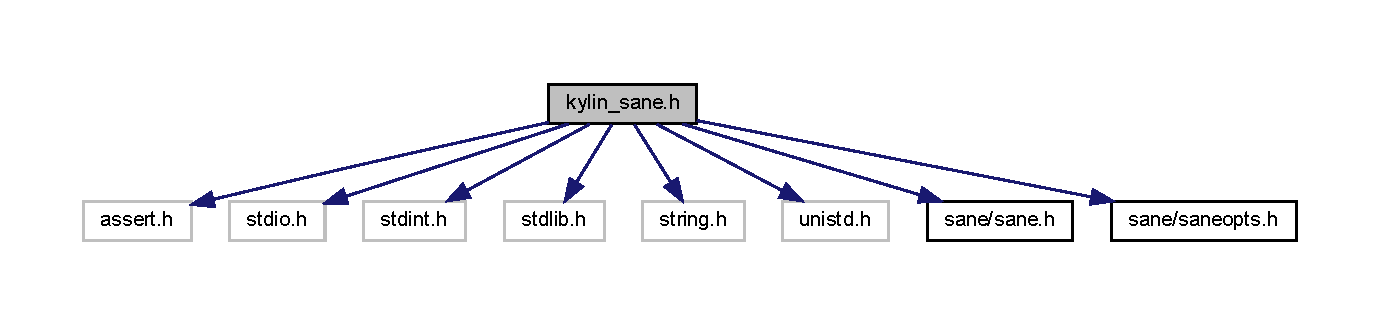
\includegraphics[width=350pt]{kylin__sane_8h__incl}
\end{center}
\end{figure}
此图展示该文件直接或间接的被哪些文件引用了\+:\nopagebreak
\begin{figure}[H]
\begin{center}
\leavevmode
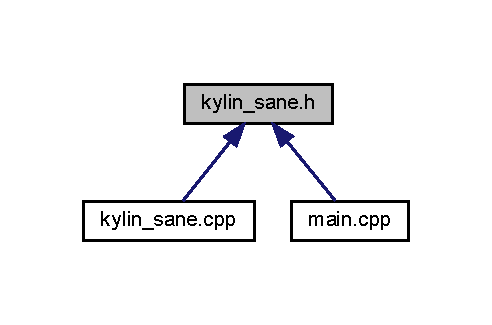
\includegraphics[width=216pt]{kylin__sane_8h__dep__incl}
\end{center}
\end{figure}
\doxysubsection*{宏定义}
\begin{DoxyCompactItemize}
\item 
\#define \mbox{\hyperlink{kylin__sane_8h_ae688d728e1acdfe5988c7db45d6f0166}{P\+A\+T\+H\+\_\+\+M\+AX}}~1024
\end{DoxyCompactItemize}
\doxysubsection*{函数}
\begin{DoxyCompactItemize}
\item 
void \mbox{\hyperlink{kylin__sane_8h_a02fd73d861ef2e4aabb38c0c9ff82947}{init}} ()
\item 
\mbox{\hyperlink{sane_8h_ae5ce8ba47cee42542d1a981be4e4c552}{S\+A\+N\+E\+\_\+\+Status}} \mbox{\hyperlink{kylin__sane_8h_a2a7c1f5e91c82fa924d2518001ff2a10}{get\+\_\+devices}} (const \mbox{\hyperlink{structSANE__Device}{S\+A\+N\+E\+\_\+\+Device}} $\ast$$\ast$$\ast$device\+\_\+list)
\item 
\mbox{\hyperlink{sane_8h_ae5ce8ba47cee42542d1a981be4e4c552}{S\+A\+N\+E\+\_\+\+Status}} \mbox{\hyperlink{kylin__sane_8h_a0c1f490d9734e1b28fdc8954c4502825}{open\+\_\+device}} (\mbox{\hyperlink{structSANE__Device}{S\+A\+N\+E\+\_\+\+Device}} $\ast$\mbox{\hyperlink{kylin__sane_8c_a9d8d7a78e723d1835dcc546917ff1784}{device}}, \mbox{\hyperlink{sane_8h_adff38d40c72e14125709194edfd45e1b}{S\+A\+N\+E\+\_\+\+Handle}} $\ast$sane\+\_\+handle)
\item 
\mbox{\hyperlink{sane_8h_ae5ce8ba47cee42542d1a981be4e4c552}{S\+A\+N\+E\+\_\+\+Status}} \mbox{\hyperlink{kylin__sane_8h_a2b640f15a12501131e316d17025fb5ac}{start\+\_\+scan}} (\mbox{\hyperlink{sane_8h_adff38d40c72e14125709194edfd45e1b}{S\+A\+N\+E\+\_\+\+Handle}} sane\+\_\+handle, \mbox{\hyperlink{sane_8h_a9a47323dab2a36db080f1bcc11585af4}{S\+A\+N\+E\+\_\+\+String\+\_\+\+Const}} file\+Name)
\item 
void \mbox{\hyperlink{kylin__sane_8h_ad9f4ca655267f3a703c60fd3e876cc63}{cancle\+\_\+scan}} (\mbox{\hyperlink{sane_8h_adff38d40c72e14125709194edfd45e1b}{S\+A\+N\+E\+\_\+\+Handle}} sane\+\_\+handle)
\item 
void \mbox{\hyperlink{kylin__sane_8h_a8550d3bcc382a085ca06334733742949}{close\+\_\+device}} (\mbox{\hyperlink{sane_8h_adff38d40c72e14125709194edfd45e1b}{S\+A\+N\+E\+\_\+\+Handle}} sane\+\_\+handle)
\item 
void \mbox{\hyperlink{kylin__sane_8h_a82ecc8db19b2f6268059b949233deaeb}{my\+\_\+sane\+\_\+exit}} ()
\end{DoxyCompactItemize}


\doxysubsection{宏定义说明}
\mbox{\Hypertarget{kylin__sane_8h_ae688d728e1acdfe5988c7db45d6f0166}\label{kylin__sane_8h_ae688d728e1acdfe5988c7db45d6f0166}} 
\index{kylin\_sane.h@{kylin\_sane.h}!PATH\_MAX@{PATH\_MAX}}
\index{PATH\_MAX@{PATH\_MAX}!kylin\_sane.h@{kylin\_sane.h}}
\doxysubsubsection{\texorpdfstring{PATH\_MAX}{PATH\_MAX}}
{\footnotesize\ttfamily \#define P\+A\+T\+H\+\_\+\+M\+AX~1024}



\doxysubsection{函数说明}
\mbox{\Hypertarget{kylin__sane_8h_ad9f4ca655267f3a703c60fd3e876cc63}\label{kylin__sane_8h_ad9f4ca655267f3a703c60fd3e876cc63}} 
\index{kylin\_sane.h@{kylin\_sane.h}!cancle\_scan@{cancle\_scan}}
\index{cancle\_scan@{cancle\_scan}!kylin\_sane.h@{kylin\_sane.h}}
\doxysubsubsection{\texorpdfstring{cancle\_scan()}{cancle\_scan()}}
{\footnotesize\ttfamily void cancle\+\_\+scan (\begin{DoxyParamCaption}\item[{\mbox{\hyperlink{sane_8h_adff38d40c72e14125709194edfd45e1b}{S\+A\+N\+E\+\_\+\+Handle}}}]{sane\+\_\+handle }\end{DoxyParamCaption})}

函数调用图\+:\nopagebreak
\begin{figure}[H]
\begin{center}
\leavevmode
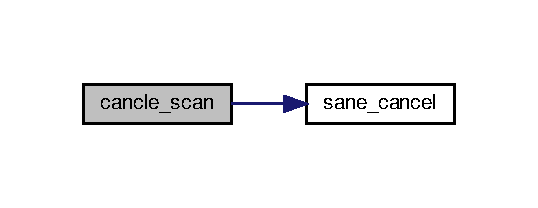
\includegraphics[width=258pt]{kylin__sane_8h_ad9f4ca655267f3a703c60fd3e876cc63_cgraph}
\end{center}
\end{figure}
这是这个函数的调用关系图\+:\nopagebreak
\begin{figure}[H]
\begin{center}
\leavevmode
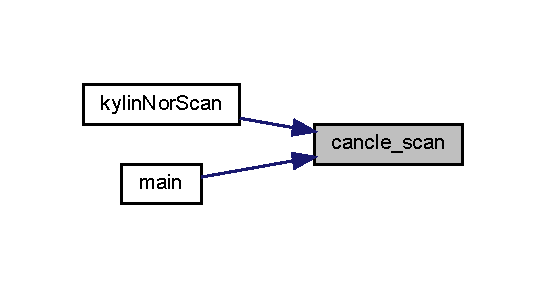
\includegraphics[width=225pt]{kylin__sane_8h_ad9f4ca655267f3a703c60fd3e876cc63_icgraph}
\end{center}
\end{figure}
\mbox{\Hypertarget{kylin__sane_8h_a8550d3bcc382a085ca06334733742949}\label{kylin__sane_8h_a8550d3bcc382a085ca06334733742949}} 
\index{kylin\_sane.h@{kylin\_sane.h}!close\_device@{close\_device}}
\index{close\_device@{close\_device}!kylin\_sane.h@{kylin\_sane.h}}
\doxysubsubsection{\texorpdfstring{close\_device()}{close\_device()}}
{\footnotesize\ttfamily void close\+\_\+device (\begin{DoxyParamCaption}\item[{\mbox{\hyperlink{sane_8h_adff38d40c72e14125709194edfd45e1b}{S\+A\+N\+E\+\_\+\+Handle}}}]{sane\+\_\+handle }\end{DoxyParamCaption})}

函数调用图\+:\nopagebreak
\begin{figure}[H]
\begin{center}
\leavevmode
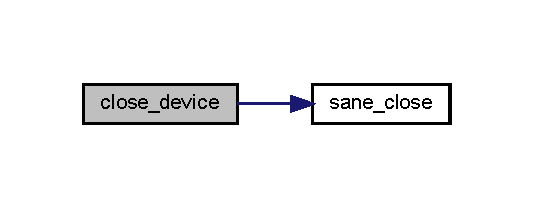
\includegraphics[width=256pt]{kylin__sane_8h_a8550d3bcc382a085ca06334733742949_cgraph}
\end{center}
\end{figure}
这是这个函数的调用关系图\+:\nopagebreak
\begin{figure}[H]
\begin{center}
\leavevmode
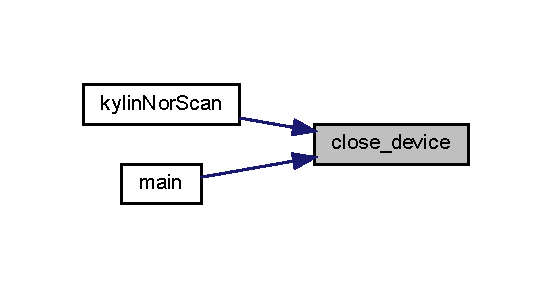
\includegraphics[width=228pt]{kylin__sane_8h_a8550d3bcc382a085ca06334733742949_icgraph}
\end{center}
\end{figure}
\mbox{\Hypertarget{kylin__sane_8h_a2a7c1f5e91c82fa924d2518001ff2a10}\label{kylin__sane_8h_a2a7c1f5e91c82fa924d2518001ff2a10}} 
\index{kylin\_sane.h@{kylin\_sane.h}!get\_devices@{get\_devices}}
\index{get\_devices@{get\_devices}!kylin\_sane.h@{kylin\_sane.h}}
\doxysubsubsection{\texorpdfstring{get\_devices()}{get\_devices()}}
{\footnotesize\ttfamily \mbox{\hyperlink{sane_8h_ae5ce8ba47cee42542d1a981be4e4c552}{S\+A\+N\+E\+\_\+\+Status}} get\+\_\+devices (\begin{DoxyParamCaption}\item[{const \mbox{\hyperlink{structSANE__Device}{S\+A\+N\+E\+\_\+\+Device}} $\ast$$\ast$$\ast$}]{device\+\_\+list }\end{DoxyParamCaption})}

函数调用图\+:\nopagebreak
\begin{figure}[H]
\begin{center}
\leavevmode
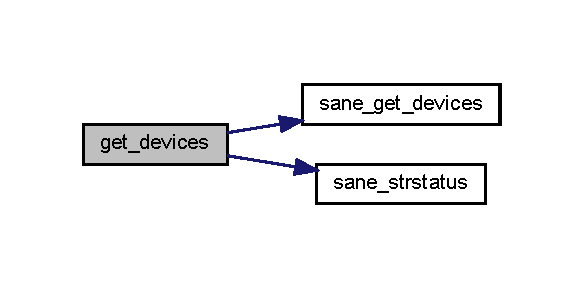
\includegraphics[width=280pt]{kylin__sane_8h_a2a7c1f5e91c82fa924d2518001ff2a10_cgraph}
\end{center}
\end{figure}
这是这个函数的调用关系图\+:\nopagebreak
\begin{figure}[H]
\begin{center}
\leavevmode
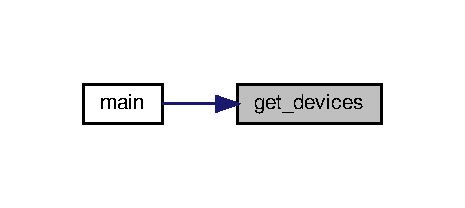
\includegraphics[width=223pt]{kylin__sane_8h_a2a7c1f5e91c82fa924d2518001ff2a10_icgraph}
\end{center}
\end{figure}
\mbox{\Hypertarget{kylin__sane_8h_a02fd73d861ef2e4aabb38c0c9ff82947}\label{kylin__sane_8h_a02fd73d861ef2e4aabb38c0c9ff82947}} 
\index{kylin\_sane.h@{kylin\_sane.h}!init@{init}}
\index{init@{init}!kylin\_sane.h@{kylin\_sane.h}}
\doxysubsubsection{\texorpdfstring{init()}{init()}}
{\footnotesize\ttfamily void init (\begin{DoxyParamCaption}{ }\end{DoxyParamCaption})}

Initialize S\+A\+NE 函数调用图\+:\nopagebreak
\begin{figure}[H]
\begin{center}
\leavevmode
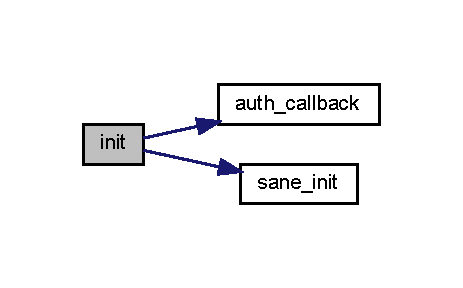
\includegraphics[width=222pt]{kylin__sane_8h_a02fd73d861ef2e4aabb38c0c9ff82947_cgraph}
\end{center}
\end{figure}
这是这个函数的调用关系图\+:\nopagebreak
\begin{figure}[H]
\begin{center}
\leavevmode
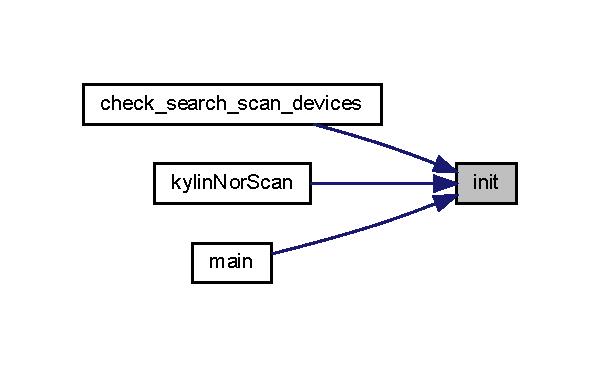
\includegraphics[width=183pt]{kylin__sane_8h_a02fd73d861ef2e4aabb38c0c9ff82947_icgraph}
\end{center}
\end{figure}
\mbox{\Hypertarget{kylin__sane_8h_a82ecc8db19b2f6268059b949233deaeb}\label{kylin__sane_8h_a82ecc8db19b2f6268059b949233deaeb}} 
\index{kylin\_sane.h@{kylin\_sane.h}!my\_sane\_exit@{my\_sane\_exit}}
\index{my\_sane\_exit@{my\_sane\_exit}!kylin\_sane.h@{kylin\_sane.h}}
\doxysubsubsection{\texorpdfstring{my\_sane\_exit()}{my\_sane\_exit()}}
{\footnotesize\ttfamily void my\+\_\+sane\+\_\+exit (\begin{DoxyParamCaption}{ }\end{DoxyParamCaption})}

函数调用图\+:\nopagebreak
\begin{figure}[H]
\begin{center}
\leavevmode
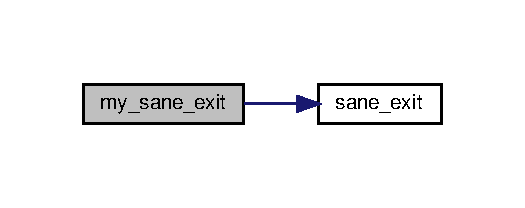
\includegraphics[width=252pt]{kylin__sane_8h_a82ecc8db19b2f6268059b949233deaeb_cgraph}
\end{center}
\end{figure}
这是这个函数的调用关系图\+:\nopagebreak
\begin{figure}[H]
\begin{center}
\leavevmode
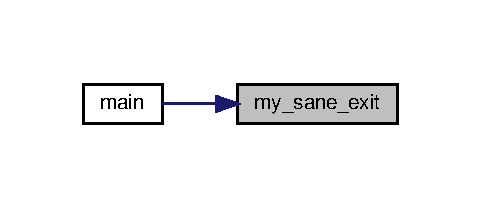
\includegraphics[width=231pt]{kylin__sane_8h_a82ecc8db19b2f6268059b949233deaeb_icgraph}
\end{center}
\end{figure}
\mbox{\Hypertarget{kylin__sane_8h_a0c1f490d9734e1b28fdc8954c4502825}\label{kylin__sane_8h_a0c1f490d9734e1b28fdc8954c4502825}} 
\index{kylin\_sane.h@{kylin\_sane.h}!open\_device@{open\_device}}
\index{open\_device@{open\_device}!kylin\_sane.h@{kylin\_sane.h}}
\doxysubsubsection{\texorpdfstring{open\_device()}{open\_device()}}
{\footnotesize\ttfamily \mbox{\hyperlink{sane_8h_ae5ce8ba47cee42542d1a981be4e4c552}{S\+A\+N\+E\+\_\+\+Status}} open\+\_\+device (\begin{DoxyParamCaption}\item[{\mbox{\hyperlink{structSANE__Device}{S\+A\+N\+E\+\_\+\+Device}} $\ast$}]{device,  }\item[{\mbox{\hyperlink{sane_8h_adff38d40c72e14125709194edfd45e1b}{S\+A\+N\+E\+\_\+\+Handle}} $\ast$}]{sane\+\_\+handle }\end{DoxyParamCaption})}

函数调用图\+:\nopagebreak
\begin{figure}[H]
\begin{center}
\leavevmode
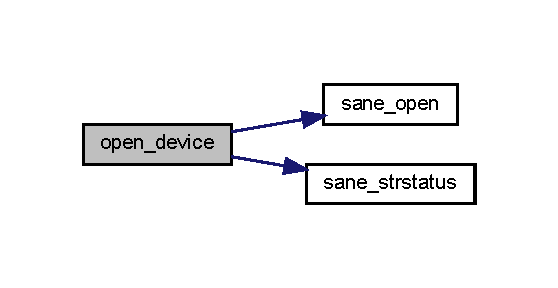
\includegraphics[width=268pt]{kylin__sane_8h_a0c1f490d9734e1b28fdc8954c4502825_cgraph}
\end{center}
\end{figure}
这是这个函数的调用关系图\+:\nopagebreak
\begin{figure}[H]
\begin{center}
\leavevmode
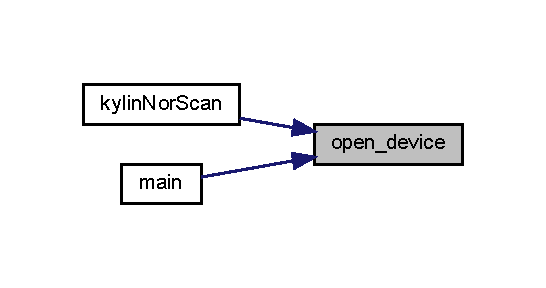
\includegraphics[width=225pt]{kylin__sane_8h_a0c1f490d9734e1b28fdc8954c4502825_icgraph}
\end{center}
\end{figure}
\mbox{\Hypertarget{kylin__sane_8h_a2b640f15a12501131e316d17025fb5ac}\label{kylin__sane_8h_a2b640f15a12501131e316d17025fb5ac}} 
\index{kylin\_sane.h@{kylin\_sane.h}!start\_scan@{start\_scan}}
\index{start\_scan@{start\_scan}!kylin\_sane.h@{kylin\_sane.h}}
\doxysubsubsection{\texorpdfstring{start\_scan()}{start\_scan()}}
{\footnotesize\ttfamily \mbox{\hyperlink{sane_8h_ae5ce8ba47cee42542d1a981be4e4c552}{S\+A\+N\+E\+\_\+\+Status}} start\+\_\+scan (\begin{DoxyParamCaption}\item[{\mbox{\hyperlink{sane_8h_adff38d40c72e14125709194edfd45e1b}{S\+A\+N\+E\+\_\+\+Handle}}}]{sane\+\_\+handle,  }\item[{\mbox{\hyperlink{sane_8h_a9a47323dab2a36db080f1bcc11585af4}{S\+A\+N\+E\+\_\+\+String\+\_\+\+Const}}}]{file\+Name }\end{DoxyParamCaption})}

函数调用图\+:\nopagebreak
\begin{figure}[H]
\begin{center}
\leavevmode
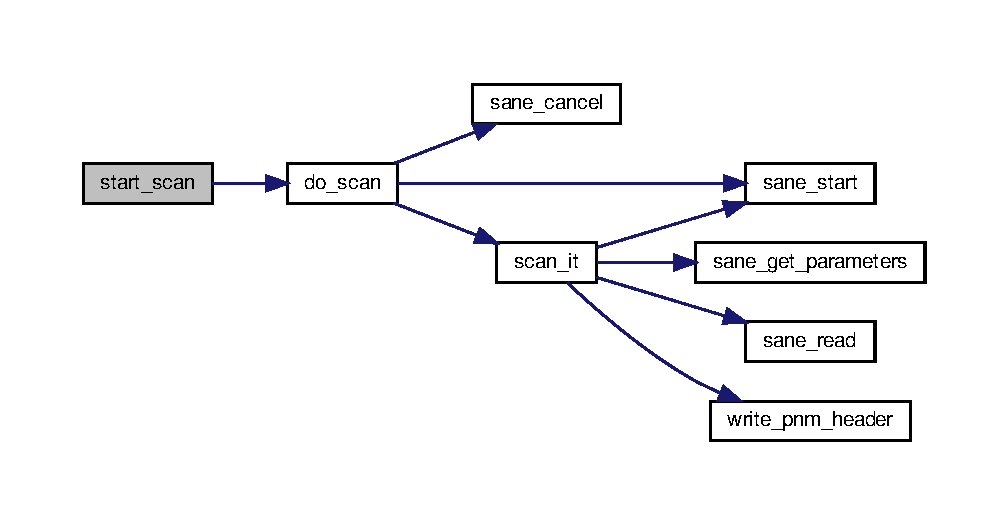
\includegraphics[width=350pt]{kylin__sane_8h_a2b640f15a12501131e316d17025fb5ac_cgraph}
\end{center}
\end{figure}
这是这个函数的调用关系图\+:\nopagebreak
\begin{figure}[H]
\begin{center}
\leavevmode
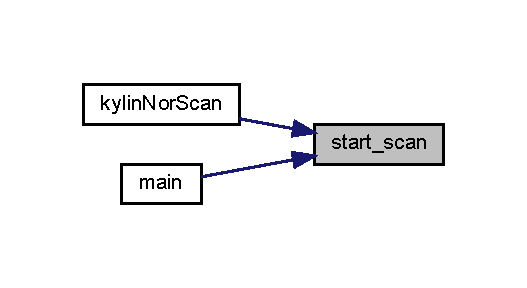
\includegraphics[width=216pt]{kylin__sane_8h_a2b640f15a12501131e316d17025fb5ac_icgraph}
\end{center}
\end{figure}

\hypertarget{main_8c}{}\doxysection{main.\+c 文件参考}
\label{main_8c}\index{main.c@{main.c}}
{\ttfamily \#include \char`\"{}kylin\+\_\+sane.\+h\char`\"{}}\newline
main.\+c 的引用(Include)关系图\+:\nopagebreak
\begin{figure}[H]
\begin{center}
\leavevmode
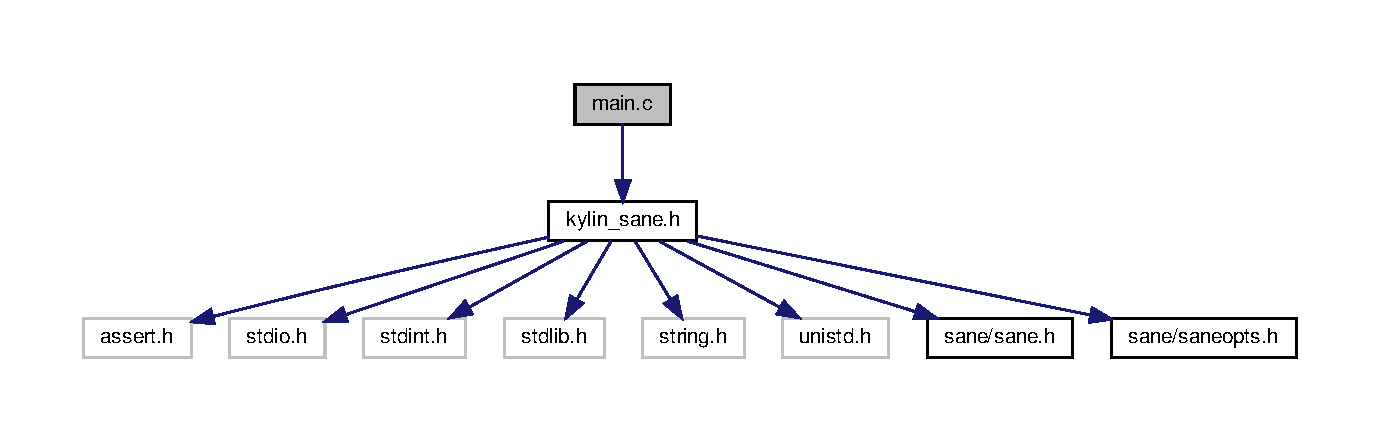
\includegraphics[width=350pt]{main_8c__incl}
\end{center}
\end{figure}
\doxysubsection*{函数}
\begin{DoxyCompactItemize}
\item 
int \mbox{\hyperlink{main_8c_ae66f6b31b5ad750f1fe042a706a4e3d4}{main}} ()
\end{DoxyCompactItemize}


\doxysubsection{函数说明}
\mbox{\Hypertarget{main_8c_ae66f6b31b5ad750f1fe042a706a4e3d4}\label{main_8c_ae66f6b31b5ad750f1fe042a706a4e3d4}} 
\index{main.c@{main.c}!main@{main}}
\index{main@{main}!main.c@{main.c}}
\doxysubsubsection{\texorpdfstring{main()}{main()}}
{\footnotesize\ttfamily int main (\begin{DoxyParamCaption}{ }\end{DoxyParamCaption})}

函数调用图\+:\nopagebreak
\begin{figure}[H]
\begin{center}
\leavevmode
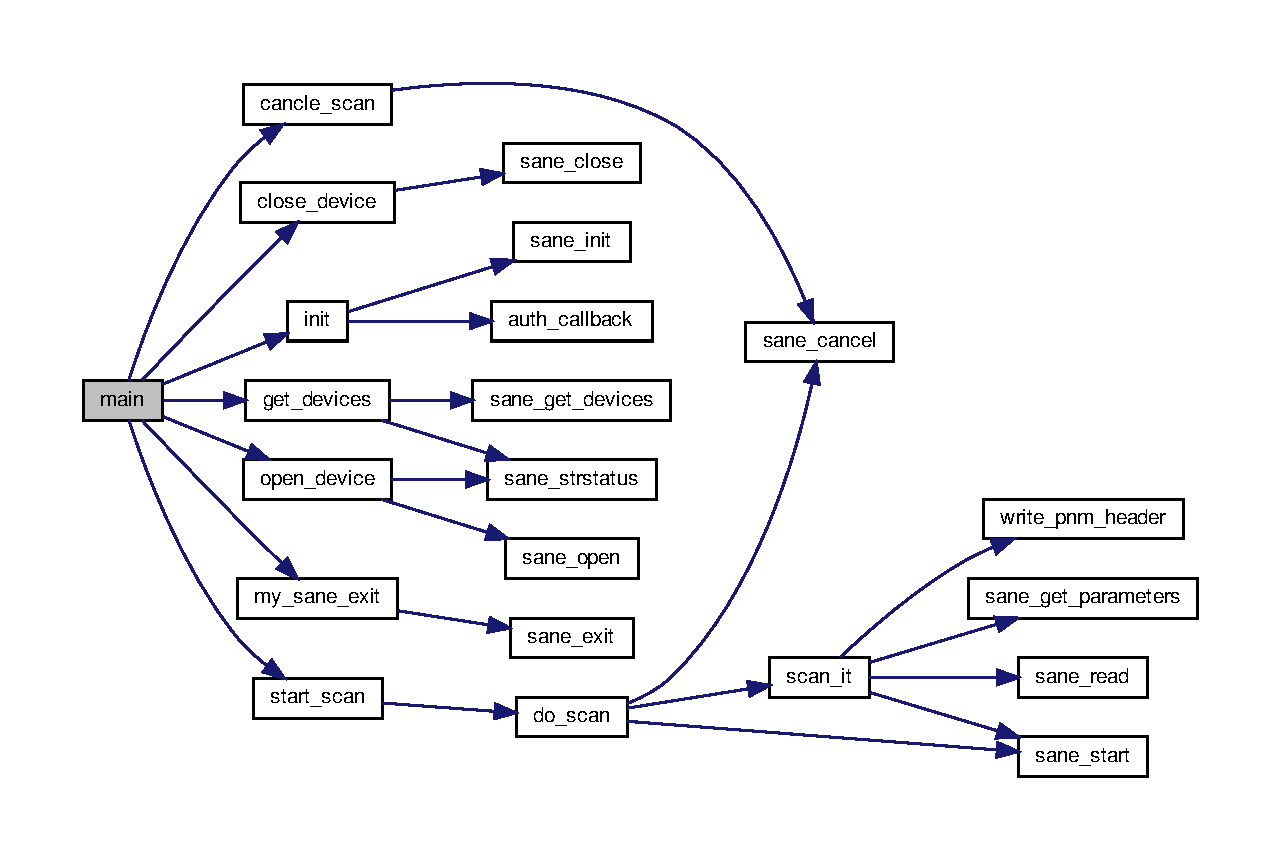
\includegraphics[width=350pt]{main_8c_ae66f6b31b5ad750f1fe042a706a4e3d4_cgraph}
\end{center}
\end{figure}

\hypertarget{README_8md}{}\section{R\+E\+A\+D\+M\+E.\+md 文件参考}
\label{README_8md}\index{R\+E\+A\+D\+M\+E.\+md@{R\+E\+A\+D\+M\+E.\+md}}

\hypertarget{README__CN_8md}{}\section{R\+E\+A\+D\+M\+E\+\_\+\+C\+N.\+md 文件参考}
\label{README__CN_8md}\index{R\+E\+A\+D\+M\+E\+\_\+\+C\+N.\+md@{R\+E\+A\+D\+M\+E\+\_\+\+C\+N.\+md}}

%--- End generated contents ---

% Index
\backmatter
\newpage
\phantomsection
\clearemptydoublepage
\addcontentsline{toc}{chapter}{索引}
\printindex

\end{document}
